\documentclass[german]{htwg-report}

\addbibresource{./bib/report.bib}
\backgroundsetup{contents={}}

\newacronym{AD}{AD}{Aggregation Derivation}
\newacronym{AHP}{AHP}{Analytic Hierarchy Process}
\newacronym{AI}{AI}{Artificial Intelligence}
\newacronym{CKAN}{CKAN}{Comprehensive Knowledge Archive Network}
\newacronym{CSV}{CSV}{Comma-Separated Values}
\newacronym{DCAT}{DCAT}{Data Catalog Vocabulary}
\newacronym{DCATAP}{DCAT-AP}{Data Catalog Vocabulary Application Profile}
\newacronym{DCATAPDE}{DCAT-AP.de}{Data Catalog Vocabulary Application Profile for Germany}
\newacronym{DQV}{DQV}{Data Quality Vocabulary}
\newacronym{FAIR}{FAIR}{Findable, Accessible, Interoperable, and Reusable}
\newacronym{FITKO}{FITKO}{Föderale IT-Kooperation}
\newacronym{GND}{GND}{Gemeinsame Normdatei}
\newacronym{HTTP}{HTTP}{Hypertext Transfer Protocol}
\newacronym{IANA}{IANA}{Internet Assigned Numbers Authority}
\newacronym{IEC}{IEC}{International Electrotechnical Commission}
\newacronym{ISO}{ISO}{International Organization for Standardization}
\newacronym{KI}{KI}{Künstliche Intelligenz}
\newacronym{LOD}{LOD}{Linked Open Data}
\newacronym{MQA}{MQA}{Metadata Quality Assessment}
\newacronym{NISO}{NISO}{National Information Standards Organization}
\newacronym{ODP}{ODP}{Open Data Portal}
\newacronym{ODPQ}{ODPQ}{Open Data Portal Quality}
\newacronym{OECD}{OECD}{Organisation for Economic Co-operation and Development}
\newacronym{OGD}{OGD}{Open Government Data}
\newacronym{RDF}{RDF}{Resource Description Framework}
\newacronym{SHACL}{SHACL}{Shapes Constraint Language}
\newacronym{SKOS}{SKOS}{Simple Knowledge Organization System}
\newacronym{SPARQL}{SPARQL}{SPARQL Protocol and RDF Query Language}
\newacronym{URI}{URI}{Uniform Resource Identifier}
\newacronym{URL}{URL}{Uniform Resource Locator}
\newacronym{W3C}{W3C}{World Wide Web Consortium}
\newacronym{XML}{XML}{Extensible Markup Language}

\begin{document}

%% Use Roman numerals for the page numbers of the title pages and table of
%% contents.
%\frontmatter
%% 'reporttype' add background elements to the cover / front page
%% possible values are:
%% bachelor	--> B S C
%% master	--> M S C
%% other		--> none
\reporttype{master}

\reporttypetext{Master-Thesis}

\title[Qualitätsmessung von Metadaten nach DCAT-AP.de Standard]{Qualitätsmessung von Metadaten nach DCAT-AP.de Standard}

\author{Lars Bürger}
\studentnumber{301662}
\studentemail{lars.buerger@htwg-konstanz.de}

\doclocation{Konstanz}
\docdate{30.09.2026}

% \makecover[]
%          
%% Include an optional title page.
\begin{titlepage}
\newgeometry{hscale=0.81,vscale=0.8}
 
\AddToShipoutPicture*{\BackgroundImgTitelPage}
 
\vspace*{12\bigskipamount}
 
 
%% Print the title in htwg-teal.
{\makeatletter
\fboxsep=0pt
\colorbox{htwg-white}{\begin{minipage}[t]{145mm}
    \begin{flushleft}
        %% Print Report Type Text
        \color{htwg-teal}\Huge{\@report@typetext}
        \\
        %% Print Report Title
        \color{htwg-teal}\Huge\textbf{\@title}
    \end{flushleft}
\end{minipage}}
\makeatother}
 
\bigskip
\bigskip
 
von
%door
 
\bigskip
\bigskip
 
%% Print the name of the author.
{\makeatletter
\Large\bfseries\@author
\makeatother}
 
\vfill
 
als Teil der Voraussetzungen f\"ur den Titel
 
\bigskip
\bigskip
 
{\bfseries Master of Science}
 
in Informatik
 
\bigskip
\bigskip
 
an der Hochschule Konstanz Technik, Wirtschaft und Gestaltung.
 
\vfill
 
\begingroup
\renewcommand*{\arraystretch}{1}
\rowcolors{2}{white}{white}
{\makeatletter
\begin{tabular}{lll}
    Matrikelnummer: & \@student@number \\ \\
    Abgabedatum: & \@doc@date \\ \\
    Betreuer: & \textbf{Prof.\ Dr.\ Markus Eiglsperger} \\
    2. Betreuer: & \textbf{Stephanie Bornholdt}
\end{tabular}
\makeatother}
\endgroup
 
\bigskip
\bigskip
 
%% reset page margins
\newgeometry{hscale=0.7,vscale=0.8}
\end{titlepage}

\tableofcontents

%% Use Arabic numerals for the page numbers of the chapters.
%\mainmatter
\pagebreak

\chapter{Einleitung}

\section{Problemstellung und Motivation}


In den vergangenen Jahren hat die Bereitstellung offener Verwaltungsdaten im Rahmen von Open Government Data (OGD) zunehmend an Bedeutung gewonnen. Durch die Veröffentlichung öffentlich finanzierter Daten sollen Transparenz, Innovation und wissenschaftliche Nutzung gefördert werden. Offene Daten können dabei neue wirtschaftliche und gesellschaftliche Mehrwerte schaffen, indem sie Forschung, datenbasierte Anwendungen und evidenzbasierte Entscheidungsprozesse unterstützen \cite{lnenicka2023}.

In Deutschland erfolgt die zentrale Bereitstellung von Metadaten zu offenen Verwaltungsdaten über das nationale Datenportal GovData. GovData fungiert als übergreifender Metadatenkatalog, über den Bund, Länder und Kommunen ihre offenen Datensätze auffindbar machen und einen zentralen Zugang zu Verwaltungsdaten bereitstellen \cite{govdata_portal, FitkoGovdata}. Die eigentlichen Datensätze werden dabei weiterhin von den jeweiligen Datenbereitstellern dezentral verwaltet, während das Portal die zugehörigen Metadaten aggregiert und über standardisierte Schnittstellen zugänglich macht.

Für die Auffindbarkeit und Nachnutzbarkeit dieser Daten spielt die Qualität der Metadaten eine zentrale Rolle. Unvollständige, inkonsistente oder fehlerhafte Metadaten können die Nutzung offener Daten erheblich erschweren und damit den Nutzen von Open-Data-Initiativen reduzieren. Vor diesem Hintergrund gewinnt die systematische Bewertung und Verbesserung der Metadatenqualität in Open-Data-Portalen zunehmend an Bedeutung.

\section{Zielsetzung der Arbeit}

Ziel dieser Masterthesis ist die Entwicklung und Evaluation eines strukturierten Verfahrens zur Bewertung und zum Reporting der Qualität von Metadaten im Kontext von GovData auf Basis des \acrfull{DCATAPDE} Standarts. Ausgangspunkt bilden Validierungsergebnisse, die mithilfe eines bestehenden RDF-/SHACL-Validators erzeugt wurden. Diese liefern formale Aussagen über strukturelle und syntaktische Eigenschaften der Metadaten, erlauben jedoch keine aggregierte oder kontextualisierte Qualitätsbewertung.
Die Thesis verfolgt daher das Ziel, aus vorhandenen Validierungsmetriken ein transparentes und praxisrelevantes Bewertungsmodell abzuleiten. Hierzu wird zunächst der Forschungsstand zu Datenqualität, Metadatenqualität sowie Bewertungsansätzen im Bereich Linked Data und Open Government Data analysiert, um geeignete Qualitätsdimen- sionen und Metriken zu identifizieren.
Dabei wird insbesondere untersucht, ob bestehende Ranking- oder Scoring-Modelle für \acrfull{DCAT}, DCAT-AP und DCAT-AP.de existieren und inwiefern diese auf den deutschen Metadatenkatalog (GovData) übertragbar sind.
Darauf aufbauend wird ein konzeptionelles Bewertungsverfahren entwickelt, das Validierungsergebnisse zu interpretierbaren Qualitätsindikatoren aggregiert. Ergänzend wird untersucht, inwiefern KI-gestützte Verfahren eingesetzt werden können, um Validierungsergebnisse zu interpretieren, zusätzliche Kontextinformationen aus Metadaten zu berücksichtigen und daraus verbesserte Qualitätsbewertungen abzuleiten. Ein möglicher Ansatz besteht dabei in der Nutzung agentenbasierter Architekturen, in denen spezialisierte KI-Agenten unterschiedliche Analyseaufgaben, etwa die Interpretation von Validierungsverletzungen oder die semantische Analyse von Metadatenfeldern, übernehmen.
Die entwickelten Metriken und Analyseverfahren werden prototypisch umgesetzt, auf repräsentative Metadatensätze angewendet und hinsichtlich ihrer Aussagekraft und praktischen Anwendbarkeit evaluiert. Ziel ist es, die rein formale RDF-Validierung um ein kontextsensitives und nachvollziehbares Qualitätsbewertungs- und Reportingsystem zu erweitern, das regelbasierte Validierung mit KI-gestützten Analyseverfahren kombiniert.

\section{Forschungsfragen}
\label{sec:forschungsfragen}

Ausgehend vom dargestellten Forschungsstand zeigt sich, dass zwar zahlreiche Modelle und technische Verfahren zur Bewertung von Daten- und Metadatenqualität existieren, deren Übertragbarkeit auf den spezifischen Kontext von DCAT-AP.de und GovData jedoch gesondert untersucht werden muss. Insbesondere stellt sich die Frage, wie formale Prüfergebnisse um kontext- und semantikbezogene Qualitätsindikatoren ergänzt werden können, ohne die Nachvollziehbarkeit des Bewertungsmodells zu beeinträchtigen. Vor diesem Hintergrund lautet die zentrale Forschungsfrage dieser Arbeit:

\begin{quote}
\enquote{Wie kann ein Bewertungsmodell für die Qualität von DCAT-AP.de-Metadaten im GovData-Kontext entwickelt werden, das formale Prüfverfahren mit ergänzenden kontext- und semantikbezogenen Qualitätsindikatoren verbindet?}
\end{quote}

Zur Beantwortung dieser Leitfrage werden folgende Teilfragen untersucht:

\begin{enumerate}
    \item Inwiefern sind bestehende Ansätze zur Bewertung von Metadaten auf den Kontext von DCAT-AP.de und GovData übertragbar?

    \item Welche Qualitätsdimensionen und Indikatoren sind für die Bewertung von DCAT-AP.de-Metadaten im GovData-Kontext relevant?

    \item Welche ergänzenden kontext- und semantikbezogenen Prüfungen können das formale Qualitätsmodell sinnvoll erweitern, ohne die Nachvollziehbarkeit und Verlässlichkeit des Scorings zu gefährden?

    \item Wie kann ein mehrdimensionales Bewertungsmodell konzeptionell entwickelt und prototypisch operationalisiert werden?

    \item Wie kann ein menschenlesbares Qualitätsreporting prototypisch umgesetzt werden, das Bewertungsergebnisse und betroffene Qualitätsdimensionen nachvollziehbar darstellt?
\end{enumerate}

\section{Aufbau der Arbeit}

Es werden theoretische und konzeptionelle Grundlagen beleuchtet. In diesem Kontext werden grundlegende Konzepte wie Open Governement Data und das GovData.de Portal erklärt. Metadaten im Open-Data-Kontext sowie RDF, LinkedData und SHACL ausgearbeitet.
Aufbauend auf die theoretischen Grundlagen wird das methodische Vorgehen dieser Arbeit beleuchtet.
Im Anschluss wird das Konzept und die Operationalisierung des Metadatenqualitätsmodell definiert und ausgearbeitet.
Es wird die Zielsetzung und Anforderungen basierend auf der Literaturrecherche, Informationen aus Experteninterviews und analysierten fehlender Dimensionen definiert.
Im Anschluss wird das evaluierte Konzept prototypisch in Python implementiert.
Die Ergebnisse des Prototyps werden im letzten Kapitel evaluiert und überprüft in wiefern sich das evaluierte Konzept und damit der Prototyp eignet.

\pagebreak
\chapter{Theoretische und konzeptionelle Grundlagen}
\label{sec:chapter_02}

\section{Open Government Data und das GovData-Portal}
\label{sec:govdata_portal}

Open Data bezeichnet Daten, die frei genutzt, weiterverwendet, und weiterverbreitet werden können. \acrfull{OGD} ist die öffentliche Ausprägung dieses Konzepts und umfasst Daten und Informationen, die von staatlichen Stellen erzeugt, erhoben, oder beauftragt und unter offenen Bedingungen bereitgestellt werden. Im Zentrum stehen dabei nicht nur der Zugang zu Daten, sondern auch ihre tatsächliche Nutzbarkeit. Damit Daten als offen gelten können, müssen sie möglichst in maschinenlesbaren, nicht-proprietären Formaten, ohne diskriminierende Zugangsbeschränkungen, und unter Bedingungen bereitgestellt werden, die ihre Wiederverwendung erlauben. OGD ist damit mehr als die bloße Veröffentlichung staatlicher Informationen im Internet; gemeint ist die proaktive Bereitstellung wiederverwendbarer Datenbestände des öffentlichen Sektors. \cite{Ubaldi2013OGD, OECD2020OURdata}

Die Relevanz von OGD begründet sich vor allem mit seinem Beitrag zu Transparenz, Partizipation, Innovation, und öffentlicher Wertschöpfung. Durch die Veröffentlichung staatlicher Daten können Bürger, Medien, Wissenschaft, Zivilgesellschaft, und Unternehmen staatliches Handeln besser nachvollziehen, kontrollieren, und analysieren. OGD kann damit Transparenz und Rechenschaft stärken und zugleich neue Formen gesellschaftlicher Beteiligung unterstützen. Darüber hinaus eröffnet es die Möglichkeit, aus vorhandenen staatlichen Daten neue Anwendungen, Dienstleistungen, und Informationsangebote zu entwickeln. Offene Regierungsdaten werden daher nicht nur als Mittel demokratischer Kontrolle verstanden, sondern auch als Ressource für wirtschaftliche und soziale Innovation. \cite{Ubaldi2013OGD}

Datenpolitik ist demnach dann wirksam, wenn sie sich nicht nur auf die Angebotsseite fokussiert, sondern auch Nutzungsbedürftnisse, Datenqualität, Metadaten, und Wiederverwendungsbedingungen berücksichtigt. OGD ist deshalb ein zentrales Element moderner datengetriebener Verwaltung: Es unterstützt Transparenz und gute Regierungsführung, kann innovative und bürgerzentrierte Dienste fördern, und bildet zugleich eine wichtige Grundlage für datenbasierte Entscheidungen im öffentlichen Sektor. Seine Relevanz ergibt sich damit aus der Verbindung von politischer Offenheit, technischer Nachnutzbarkeit, und gesellschaftlicher Wertschöpfung. \cite{OECD2020OURdata}

In Deutschland bildet GovData das nationale Metadatenportal für offene Verwaltungsdaten. Das Portal fungiert als zentraler Zugangspunkt zu Datenangeboten von Bund, Ländern, und Kommunen, verwaltet jedoch nicht die physischen Datensätze selbst. Vielmehr werden Metadaten gebündelt, über die auf die dezentral in verschiedenen Fach- und Verwaltungsportalen veröffentlichten Daten verwiesen wird. GovData übernimmt damit vor allem eine Aggregations- und Sichtbarkeitsfunktion, indem verteilte Datenbestände über einen gemeinsamen Metadatenzugang auffindbar gemacht werden. \cite{BmdsOpenData}

Im institutionellen Rahmen wird GovData von der Förderalen IT-Kooperation (FITKO) im Produktmanagement betreut.
Die FITKO ordnet das Portal ihrem einheitlichen Produktmanagement-Modell für Produkte des IT-Planungsrats zu und verweist für GovData auf ein eigenes föderal besetztes Produktboard \cite{FitkoGovdata}.

\section{Metadaten im Open-Data-Kontext}

Metadaten lassen sich in Anlehnung an die \acrfull{NISO} als Informationen verstehen, die erstellt, gespeichert, und geteilt werden, um Informationsressourcen zu beschreiben und dadurch ihren Gebrauch zu ermöglichen. Die klassische Kurzformel „data about data“ greift dabei nur verkürzt. Entscheidend ist der funktionale Aspekt: Metadaten machen eine Ressource identifizierbar, beschreibbar, auffindbar, und in einem bestimmten Nutzungskontext verständlich. NISO betont zudem, dass Metadaten typischerweise strukturiert sind, also in bekannten Kategorien erfasst werden, damit Menschen und Systeme mit ihnen arbeiten können. Für Datensätze im Open-Data-Kontext bedeutet dies, dass Metadaten nicht bloß Begleitinformationen sind, sondern die Beschreibungsschicht, über die Datensätze gefunden, eingeordnet, und verwendet werden können. \cite{Riley2017MetadataPrimer}

NISO unterscheidet grundlegend zwischen deskriptiven, administrativen, strukturellen und Markup Metaden.
Diese sind zur orientierung in Tabelle \ref{tab:metadaten_typen} aufgelistet.

\begin{table}[ht]
    \rowcolors{1}{white}{white}
    \centering
        \begin{tabular}{p{4cm}p{9.5cm}}
        \hline
        \textbf{Metadatentyp} & \textbf{Beschreibung} \\
        \hline
        Deskriptive Metadaten & Dienen der inhaltlichen Beschreibung einer Ressource und unterstützen deren Identifikation und Auffindbarkeit. \\
        Administrative Metadaten & Unterstützen die Verwaltung einer Ressource, etwa durch Angaben zu Rechten, technischen Eigenschaften, Provenienz oder Erhaltung. \\
        Strukturelle Metadaten & Beschreiben den Aufbau einer Ressource sowie die Beziehungen zwischen ihren Bestandteilen. \\
        Markup-Metadaten & Kennzeichnen die logische oder semantische Struktur innerhalb eines digitalen Objekts. \\
        \hline
        \end{tabular}
        \captionsetup{justification=centering}
        \caption[Metadatentypen in Anlehnung an NISO, eigene Übersetzung und Paraphrase]{Metadatentypen in Anlehnung an NISO, eigene Übersetzung und Paraphrase \cite{Riley2017MetadataPrimer}}
    \label{tab:metadaten_typen}
\end{table}

Im Open-Data-Kontext kommt Metadaten eine besondere Bedeutung zu, da offene Datensätze nur dann praktisch nutzbar sind, wenn sie standardisiert beschrieben und dadurch auffindbar, verständlich, und zwischen verschiedenen Katalogen interoperabel gemacht werden.
DCAT ist hierfür das zentrale W3C-Vokabular, das die interoperable Beschreibung von Datenkatalogen, Datensätzen, und Datendiensten im Web ermöglichen soll. \cite{W3CDCAT3}

In funktionaler Hinsicht lassen sich die im GovData-Kontext verwendeten Metadaten vor allem als deskriptive und administrative Metadaten einordnen, da sie einerseits der Beschreibung und Auffindbarkeit von Verwaltungsdaten dienen und andererseits Informationen zur Bereitstellung, zu Formaten, zu offenen Lizenzen, und zur Nachnutzbarkeit enthalten \cite{Riley2017MetadataPrimer,FitkoGovdata}.
Da GovData selbst als nationales Metadatenportal fungiert, einen Metadatenkatalog bereitstellt, und die beschriebenen Verwaltungsdaten weiterhin dezentral bei den bereitstellenden Stellen verbleiben, kommt dieser Beschreibungsschicht eine zentrale infrastrukturelle Funktion zu \cite{FitkoGovdata}.

\section{DCAT-AP.de als Metadatenstandard} % @TODO ggf. noch etwas expliziter erleutern wie DCAT-AP.de aufgebaut ist

Für den Austausch offener Verwaltungsdaten im deutschen Open-Data-Kontext kommt DCAT-AP.de eine zentrale Rolle zu. Der Standard definiert ein gemeinsames deutsches Metadatenmodell, mit dem Metadaten aus unterschiedlichen Open-Data-Portalen interoperabel bereitgestellt und über GovData zentral auffindbar gemacht werden können. \cite{DCATAPDEStart, DCATAPDESpec2, DCATAPDESpec3}


Für den Austausch offener Verwaltungsdaten im deutschen Open-Data-Kontext kommt dem Standard DCAT-AP.de eine zentrale Rolle zu. DCAT-AP.de ist das gemeinsame deutsche Metadatenmodell für den Austausch offener Verwaltungsdaten und dient dazu, Metadaten aus unterschiedlichen Portalen in einer einheitlichen Struktur bereitzustellen \cite{DCATAPDEStart}. Sein Zweck liegt insbesondere darin, Metadaten offener Verwaltungsdaten zwischen deutschen Open-Data-Portalen interoperabel auszutauschen und diese Daten über GovData zentral auffindbar zu machen \cite{DCATAPDESpec3,DCATAPDESpec2}. 

DCAT-AP.de ist keine isolierte nationale Eigenentwicklung, sondern eine deutsche Ableitung des europäischen Standards DCAT-AP, der wiederum auf dem W3C-Vokabular DCAT aufbaut. Damit steht der Standard in einem mehrstufigen Interoperabilitätszusammenhang: vom allgemeinen Modell für Datenkataloge im Web über das europäische Anwendungsprofil bis hin zur deutschen Spezifikation für offene Verwaltungsdaten \cite{DCATAPDEStart,DCATAPDESpec3}. Diese Einbettung ist insbesondere deshalb relevant, weil Metadaten im GovData-Kontext nicht nur innerhalb Deutschlands ausgetauscht, sondern zugleich an europäische Entwicklungen anschlussfähig bleiben sollen \cite{FitkoGovdata}. 

Die Qualität und Standartkonformität der Metadaten ist damit eine zentrale Voraussetzung dafür, dass Datensätze protalübergreifend auffindbar, maschinell verarbeitbar und interoperable nachnutzbar werden \cite{FitkoGovdata, FITKOGovDataDocs}.

Zugleich zeigt sich an DCAT-AP.de, dass Metadaten im Open-Data-Kontext nicht nur eine dokumentierende, sondern auch eine strukturierende Funktion haben. Der Standard legt fest, welche Informationen in welcher Form beschrieben werden sollen, und schafft so die Grundlage für einheitliche semantische Beschreibungen, föderierte Suche, und die Weiterverarbeitung von Metadaten über Schnittstellen und Portale hinweg \cite{DCATAPDESpec3,DCATAPDEImplRules2}. Für die vorliegende Arbeit ist DCAT-AP.de damit der maßgebliche Referenzrahmen, innerhalb dessen sich die Frage nach der Qualität von Metadaten im GovData-Kontext konkretisiert.

\subsection{Aufbau eines DCAT-AP.de-Datensatzes am Referenzdatensatz}
\label{sec:referenzdatensatz}

Wie ein nach diesem Standard beschriebener Datensatz konkret aussieht, lässt sich an einem Referenzdatensatz als Beispiel zeigen.

Grundlage ist ein realer Metadatensatz aus dem Open-Data-Portal Schleswig-Holstein, der die Tagesmittelwerte der Feinstaubbelastung des Jahres 2023 an einer Lübecker Luftmessstation beschreibt. Er wurde an den Stellen ergänzt, an denen das Original Angaben schuldig blieb, bis er sämtliche Prüfungen des in Kapitel~4 entwickelten Bewertungsmodells erfüllt. Der Datensatz ist damit ein \emph{konstruierter Idealfall}: Er zeigt, wie eine vollständige Beschreibung nach DCAT-AP.de aussieht, erlaubt aber ausdrücklich keine Aussage darüber, wie verbreitet eine solche Beschreibungstiefe in der Portalpraxis ist. Listing~\ref{lst:referenzdatensatz} zeigt ihn gekürzt, der vollständige Quelltext steht in Anhang~\ref{app:referenzdatensatz}.

\begin{listing}[H]
\begin{minted}
[
frame=lines,
framesep=2mm,
baselinestretch=1.1,
fontsize=\scriptsize,
breaklines,
breakafter=/,
breakaftersymbolpre={}
]
{xml}
<dcat:Dataset rdf:about="https://opendata.schleswig-holstein.de/dataset/39054cb0-...">
  <dct:title>Feinstaub (PM2,5) in Lübeck, Messstation Moislinger Allee: Tagesmittelwerte 2023</dct:title>
  <dct:description>Der Datensatz enthält die Tagesmittelwerte der Feinstaubkonzentration ...</dct:description>
  <dcat:keyword xml:lang="de">Feinstaub</dcat:keyword>
  <dcat:theme rdf:resource="http://publications.europa.eu/resource/authority/data-theme/ENVI"/>
  <dct:temporal>
    <dct:PeriodOfTime rdf:nodeID="temporal-2023">
      <dcat:startDate rdf:datatype="...#date">2023-01-01</dcat:startDate>
      <dcat:endDate rdf:datatype="...#date">2023-12-31</dcat:endDate>
    </dct:PeriodOfTime>
  </dct:temporal>
  <dct:spatial>
    <dct:Location rdf:nodeID="location-luebeck-moislinger-allee">
      <locn:geometry rdf:datatype="...#wktLiteral">POINT (10.6733 53.8622)</locn:geometry>
    </dct:Location>
  </dct:spatial>
  <dcat:contactPoint>
    <vcard:Organization rdf:nodeID="contact-lfu-sh">
      <vcard:fn>Landesamt für Umwelt Schleswig-Holstein, Open Data</vcard:fn>
      <vcard:hasURL rdf:resource="https://opendata.schleswig-holstein.de/organization/lfu"/>
    </vcard:Organization>
  </dcat:contactPoint>
  <dcat:distribution>
    <dcat:Distribution rdf:about="http://lfu.landsh.de/DESH053_PM25_1TMW_2023/data">
      <dct:title xml:lang="de">Tagesmittelwerte PM2,5 2023, Station Lübeck Moislinger Allee – CSV</dct:title>
      <dct:license rdf:resource="http://dcat-ap.de/def/licenses/dl-by-de/2.0"/>
      <dcat:accessURL rdf:resource="https://www.umweltbundesamt.de/api/air_data/v2/measures/csv?..."/>
      <dcat:downloadURL rdf:resource="https://www.umweltbundesamt.de/api/air_data/v2/measures/csv?..."/>
      <dcat:mediaType rdf:resource="https://www.iana.org/assignments/media-types/text/csv"/>
      <dct:format rdf:resource="http://publications.europa.eu/resource/authority/file-type/CSV"/>
      <dcatap:availability rdf:resource=".../planned-availability/STABLE"/>
    </dcat:Distribution>
  </dcat:distribution>
  <dcat:distribution>
    <dcat:Distribution rdf:about="http://lfu.landsh.de/DESH053_PM25_1TMW_2023/data.json">
      <dct:title xml:lang="de">Tagesmittelwerte PM2,5 2023, Station Lübeck Moislinger Allee – JSON</dct:title>
      <dct:format rdf:resource="http://publications.europa.eu/resource/authority/file-type/JSON"/>
      ...
    </dcat:Distribution>
  </dcat:distribution>
  <dcatde:politicalGeocodingLevelURI rdf:resource=".../politicalGeocoding/Level/municipality"/>
  <dcatde:politicalGeocodingURI rdf:resource=".../politicalGeocoding/municipalityKey/01003000"/>
  <dcatde:contributorID rdf:resource="http://dcat-ap.de/def/contributors/schleswigHolstein"/>
</dcat:Dataset>
\end{minted}
\caption{Referenzdatensatz in DCAT-AP.de, gekürzt}
\label{lst:referenzdatensatz}
\end{listing}

Zwei Strukturmerkmale prägen den Aufbau. Erstens trennt DCAT zwischen dem \texttt{dcat:Dataset} als der beschriebenen Sache und der \texttt{dcat:Distribution} als der konkret abrufbaren Repräsentation dieser Sache. Titel, Beschreibung, Schlagwörter, Thema sowie räumlicher und zeitlicher Bezug hängen am Datensatz, während Format, Medientyp, Lizenz und die Zugriffs- und Download-Adressen Eigenschaften der einzelnen Distribution sind. Ein Datensatz kann mehrere Distributionen tragen, im Regelfall denselben Inhalt in unterschiedlichen Formaten: Der Referenzdatensatz bietet die Messreihe als CSV und als JSON an, beide über dieselbe Schnittstelle des Umweltbundesamtes und mit identischem Datenbestand. Diese Trennung ist für die Qualitätsbewertung folgenreich, weil ein Teil der Prüfungen damit je Distribution und nicht je Datensatz zu erfolgen hat -- ein Punkt, auf den Abschnitt~\ref{sec:messmodell} zurückkommt.

Zweitens sind die inhaltlich entscheidenden Angaben keine freien Texte, sondern Verweise auf kontrollierte Vokabulare. Thema, Dateiformat, Medientyp, Sprache, Aktualisierungsfrequenz, Lizenz und Verfügbarkeit werden jeweils als URI aus einer vorgegebenen Liste gesetzt, überwiegend aus den Vokabularen des EU-Publikationsamts. Hinzu kommen die deutschen Erweiterungen des Profils im Namensraum \texttt{dcatde}, insbesondere die politische Geokodierung über den amtlichen Gemeindeschlüssel samt zugehöriger Ebene sowie die Kennung der liefernden Stelle. Erst diese Festlegung auf gemeinsame Wertelisten macht Metadaten portalübergreifend vergleichbar und filterbar: Ein Freitext \enquote{Umwelt} im Themenfeld wäre für eine föderierte Suche wertlos, der URI der Kategorie \texttt{ENVI} dagegen eindeutig auswertbar. Für die Qualitätsbewertung folgt daraus, dass sich ein erheblicher Teil der Prüfungen als Abgleich gegen genau diese Vokabulare formulieren lässt.

\section{RDF, Linked Data und SHACL}

RDF bildet die technische Grundlage für die Beschreibung von Metadaten im Semantic-Web-Kontext. Nach der W3C-Spezifikation ist RDF ein Modell zur Repräsentation von Informationen im Web, dessen Kernstruktur aus Subjekt-Prädikat-Objekt-Tripeln besteht, die gemeinsam als RDF-Graph modelliert werden. RDF ist damit nicht primär als konkretes Dateiformat zu verstehen, sondern als abstraktes Datenmodell, auf dem unterschiedliche RDF-basierte Sprachen und Serialisierungen aufbauen. \cite{W3CRDF11Concepts}

Für GovData ist RDF unmittelbar relevant, da die zuliefernden Stellen ihre Datenkataloge im RDF-Format und konform zum geltenden Metadatenstandard DCAT-AP.de für den Import in das Portal bereitstellen.
Die Original-Metadaten können dabei über den Endpunkt eines Triple Stores mittels SPARQL-Abfragen durchsucht und kombiniert werden.
Ein Triple Store ist eine auf RDF-Daten spezialisierte Datenbank, in der Informationen als RDF-Tripel beziehungsweise RDF-Graphen gespeichert und abgefragt werden können.
SPARQL ist die standardisierte Abfragesprache für RDF-Daten und ermöglicht es, RDF-Graphen beziehungsweise RDF-Datenbestände über Graphmuster zu durchsuchen und auszuwerten \cite{w3c_rdf11_concepts,w3c_sparql11_query}.
RDF fungiert in diesem Kontext somit als gemeinsames Modell, in dem Metadaten standardisiert beschrieben, gespeichert, und verarbeitet werden.


Die Bedeutung von RDF hängt eng mit den Prinzipien von Linked Data zusammen. Linked Data zielt darauf, Daten im Internet so zu veröffentlichen, dass sie maschinell verarbeitbar, referenzierbar, und mit anderen Datenbeständen verknüpfbar sind. Für Datenkataloge ist dies insbesondere deshalb relevant, weil Metadaten nicht nur innerhalb einzelner Portale genutzt, sondern auch katalogübergreifend aggregiert und durchsucht werden sollen. Das W3C-Vokabular DCAT ist genau für diesen Zweck konzipiert: Es soll die Interoperabilität zwischen im Web veröffentlichten Datenkatalogen erleichtern, die Aggregation von Metadaten aus mehreren Katalogen unterstützen, die Auffindbarkeit von Datensätzen erhöhen, und föderierte Suche über verschiedene Kataloge hinweg ermöglichen. \cite{W3CDCAT3}

Zur formalen Validierung von RDF-basierten Metadaten dient SHACL.
Die W3C beschreibt SHACL als eine Sprache zur Validierung von RDF-Graphen gegen eine Menge von Bedingungen, die in Form sogenannter Shapes ausgedrückt werden.
Auf diese Weise lassen sich etwa Kardinalitäten, Datentypen, Klassenzugehörigkeiten, oder Wertebereiche prüfen.
SHACL ermöglicht somit die formale Überprüfung, ob ein RDF-Datenbestand vorgegebene strukturelle und syntaktische Anforderungen erfüllt. \cite{W3CSHACL}

Gleichzeitig ist formale Validierung nicht mit umfassender Qualitätsbewertung gleichzusetzen. 
SHACL dient der Prüfung von RDF-Graphen gegen formal definierte Constraints und erlaubt damit insbesondere Aussagen über strukturelle und syntaktische Konformität \cite{W3CSHACL}.
In der Literatur zu Linked Data und Metadatenqualität wird Validierung zwar als zentraler Bestandteil der Qualitätsprüfung betrachtet, zugleich aber betont, dass darüber hinaus weitere Qualitätsdimensionen wie Vollständigkeit, Auffindbarkeit, Genauigkeit, oder Nachnutzbarkeit relevant sind \cite{Gayo2015LinkedDataValidationQuality,Neumaier2016MetadataQuality,Zaveri2016LinkedDataQuality}.
SHACL kann folglich wichtige Aussagen über Regelkonformität liefern, erfasst jedoch nicht automatisch alle Aspekte, die für die praktische Qualität von Metadaten entscheidend sind.
Dies gilt insbesondere im GovData-Kontext, in dem Metadaten nicht nur formal korrekt, sondern auch für die zentrale Auffindbarkeit und Nachnutzung dezentral bereitgestellter Verwaltungsdaten geeignet sein müssen \cite{FitkoGovdata}.

\section{Datenqualität}

Datenqualität wird in der Forschung nicht als eindimensionale Eigenschaft verstanden, sondern als mehrdimensionales Konzept, das sich erst im Verhältnis zu einem konkreten Nutzungskontext bestimmen lässt.

\subsection{Definition nach Wang and Strong 1996}
\label{sec:wang_strong_definition_quality}

Einen zentralen Referenzpunkt bildet die Arbeit von Wang und Strong, die Datenqualität als \enquote{fitness for use} definieren und damit die Perspektive der Datennutzenden in den Mittelpunkt stellen \cite{wang1996beyond}. Ausgehend von einer empirischen Untersuchung von Datenkonsumentinnen und -konsumenten entwickeln sie ein hierarchisches Rahmenmodell, in dem Datenqualitätsmerkmale nicht allein aus theoretischen Vorannahmen oder aus Sicht von Systementwickelnden abgeleitet werden, sondern aus den Anforderungen tatsächlicher Nutzungssituationen hervorgehen \cite{wang1996beyond}. Damit verschiebt sich der Fokus von einem engen Verständnis von Datenqualität als bloßer Fehlerfreiheit zu einem breiteren Verständnis, das auch Relevanz, Verständlichkeit, Zugänglichkeit, und Nutzungseignung umfasst.

Wang und Strong unterscheiden vier übergeordnete Kategorien von Datenqualität: intrinsische, kontextuelle, repräsentationale, und zugangsbezogene Qualität \cite{wang1996beyond}. Diese Kategorien bündeln insgesamt 15 untergeordnete Dimensionen und beschreiben unterschiedliche Perspektiven auf Datenqualität.

\begin{itemize}
    \item \textbf{Intrinsische Qualität} betrifft Eigenschaften, die den Daten selbst zugeschrieben werden können. Darunter befinden sich die Dimensionen \textit{Genauigkeit}, \textit{Objektivität}, \textit{Glaubwürdigkeit} und \textit{Reputation}.
    \item \textbf{Kontextuelle Qualität} verweist darauf, dass Daten nur in Relation zu einem bestimmten Verwendungszweck bewertet werden können und umfasst daher insbesondere \textit{Relevanz}, \textit{Mehrwert}, \textit{Aktualität}, \textit{Vollständigkeit} und eine \textit{angemessene Datenmenge}.
    \item \textbf{Repräsentationale Qualität} betrifft die Form der Darstellung, also \textit{Interpretierbarkeit}, \textit{Verständlichkeit}, \textit{prägnante Repräsentation} und \textit{konsistente Darstellung}.
    \item \textbf{Zugangsbezogene Qualität} beschreibt, ob Daten für ihre Nutzung überhaupt verfügbar und unter angemessenen Sicherheitsbedingungen zugänglich sind.
\end{itemize}

Qualität ist in diesem Verständnis weder vollständig inhärent noch allein technisch gegeben. Vielmehr hängt sie davon ab, ob Daten in einem bestimmten Arbeits- oder Entscheidungskontext brauchbar sind \cite{wang1996beyond}. Diese Perspektive wurde von Strong, Lee, und Wang weiter ausgebaut, die betonen, dass Datenqualitätsprobleme nicht nur in gespeicherten Daten selbst entstehen, sondern im weiteren Kontext von Informationssystemen, also auch in Produktions-, Speicher-, und Nutzungskontexten \cite{StrongLeeWang1997}.

Ergänzend zu diesem nutzungsbezogenen Rahmen schlagen Wand und Wang eine ontologische Fundierung von Datenqualität vor \cite{wand1996anchoring}. Ausgangspunkt ihres Ansatzes ist die Annahme, dass Informationssysteme reale Sachverhalte repräsentieren. Datenqualitätsprobleme lassen sich dann als Repräsentationsdefizite zwischen der beobachtbaren realen Welt und ihrer Abbildung im Informationssystem beschreiben \cite{wand1996anchoring}. Auf dieser Grundlage unterscheiden sie insbesondere Defizite wie Unvollständigkeit, Mehrdeutigkeit, Bedeutungslosigkeit, und Fehlerhaftigkeit. Der Beitrag dieses Ansatzes liegt weniger in einer nutzungsbezogenen Typologie als vielmehr in einer begrifflich präziseren theoretischen Herleitung von Qualitätsdimensionen. Während Wang und Strong den empirisch wahrgenommenen Qualitätsbedarf von Datennutzenden systematisieren, zeigen Wand und Wang, dass Datenqualität auch als Frage adäquater Repräsentation modelliert werden kann. Beide Perspektiven ergänzen sich daher: Die eine macht die Anwendungs- und Nutzerseite 
sichtbar, die andere präzisiert die begriffliche und modelltheoretische Grundlage von Qualitätsdefiziten.

\subsection{Qualitätsmodell der ISO-Norm 25012}

Ergänzend zur Definition von Wang und Strong bietet der Standard ISO/IEC 25012 einen normativen Bezugsrahmen.
Der Standard ist weiterhin aktuell und die Ausgabe von 2008 wurde von ISO im Jahr 2025 bestätigt.
Er definiert ein allgemeines Datenqualitätsmodell für strukturiert in Computersystemen gehaltene Daten.
Datenqualitätsmerkmale werden den Perspektiven inhärenter und systemabhänger Qualität zugeordnet. \cite{iso25012}

Figur \ref{fig:iso25012_quality_model_de} veranschaulicht den definierten Standard.
Das Modell umfasst 15 Qualitätsmerkmale und betont ausdrücklich, dass deren Relevanz je nach Stakeholdern und Anwendungskontext variiert.

\begin{figure}[ht]
\centering
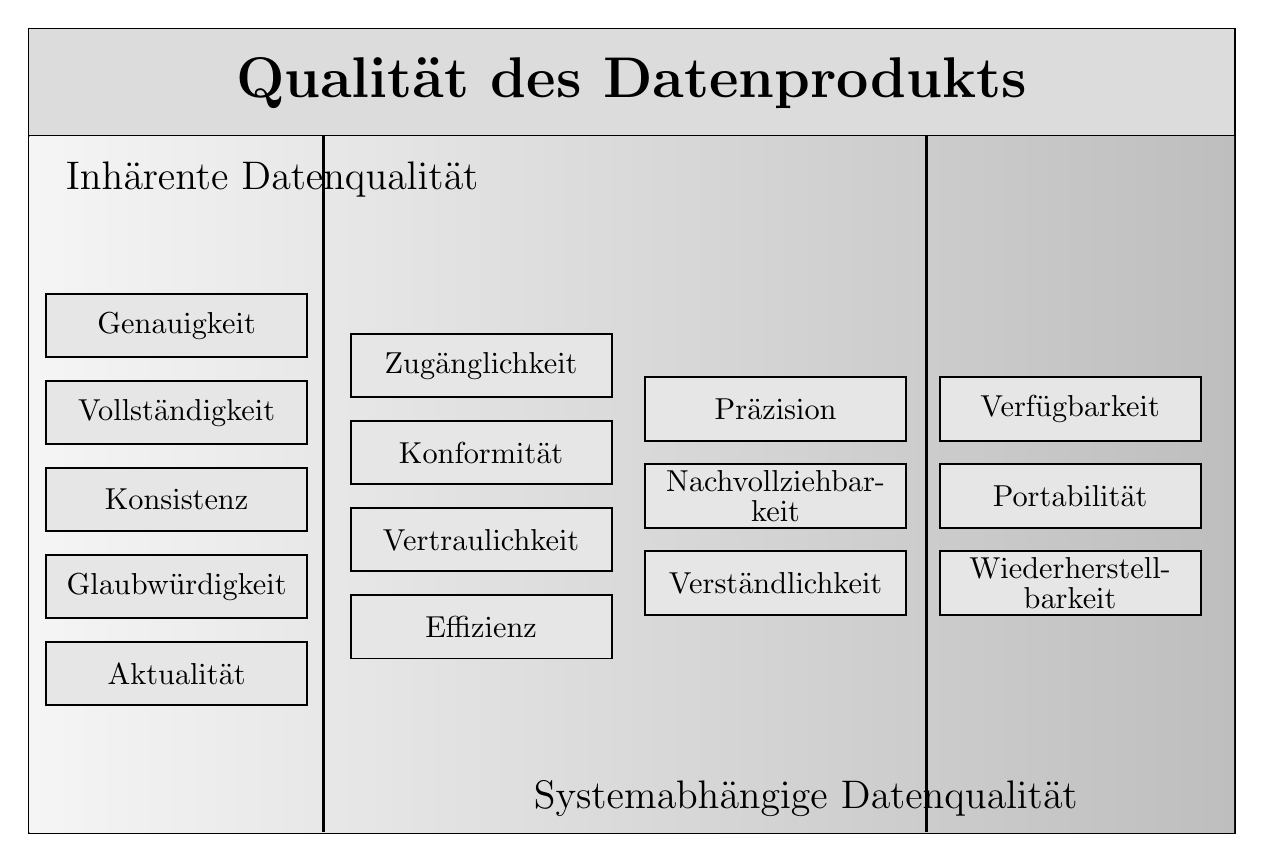
\begin{tikzpicture}[x=0.85cm,y=0.85cm, font=\sffamily]

    % Grautöne
    \definecolor{headergray}{RGB}{220,220,220}
    \definecolor{leftgray}{RGB}{245,245,245}
    \definecolor{rightgray}{RGB}{190,190,190}
    \definecolor{boxfill}{RGB}{230,230,230}

    % Maße
    \def\W{18}
    \def\H{12}
    \def\HH{1.6}

    % Außenrahmen
    \draw[line width=1.2pt] (0,0) rectangle (\W,\H);

    % Kopfzeile
    \fill[headergray] (0,\H-\HH) rectangle (\W,\H);
    \draw[line width=1.2pt] (0,\H-\HH) -- (\W,\H-\HH);

    % Hauptfläche mit grauem Verlauf
    \shade[left color=leftgray, right color=rightgray]
        (0,0) rectangle (\W,\H-\HH);

    % Vertikale Trennlinien
    \draw[line width=1pt] (4.4,0) -- (4.4,\H-\HH);
    \draw[line width=1pt] (13.4,0) -- (13.4,\H-\HH);

    % Titel
    \node[font=\bfseries\fontsize{22}{24}\selectfont] at (\W/2,\H-0.8)
        {Qualität des Datenprodukts};

    % Bereichsüberschriften
    \node[anchor=west,font=\fontsize{15}{17}\selectfont] at (0.4,9.75)
        {Inhärente Datenqualität};

    \node[font=\fontsize{15}{17}\selectfont] at (11.6,0.5)
        {Systemabhängige Datenqualität};

    % Box-Makro: breiter und mit Zeilenumbruch
    \newcommand{\ibox}[3]{%
        \draw[fill=boxfill, line width=0.7pt] (#1,#2) rectangle ++(3.9,0.95);
        \node[font=\fontsize{11}{11}\selectfont, align=center, text width=3.40cm]
            at (#1+1.95,#2+0.475) {#3};
    }

    % Linke Gruppe
    \ibox{0.25}{7.1}{Genauigkeit}
    \ibox{0.25}{5.8}{Vollständigkeit}
    \ibox{0.25}{4.5}{Konsistenz}
    \ibox{0.25}{3.2}{Glaubwürdigkeit}
    \ibox{0.25}{1.9}{Aktualität}

    % Mittlere Gruppe links
    \ibox{4.8}{6.5}{Zugänglichkeit}
    \ibox{4.8}{5.2}{Konformität}
    \ibox{4.8}{3.9}{Vertraulichkeit}
    \ibox{4.8}{2.6}{Effizienz}

    % Mittlere Gruppe rechts
    \ibox{9.2}{5.85}{Präzision}
    \ibox{9.2}{4.55}{Nachvollziehbar- \ keit}
    \ibox{9.2}{3.25}{Verständlichkeit}

    % Rechte Gruppe
    \ibox{13.6}{5.85}{Verfügbarkeit}
    \ibox{13.6}{4.55}{Portabilität}
    \ibox{13.6}{3.25}{Wiederherstell- \ barkeit}

\end{tikzpicture}
\caption[Schematische Darstellung inhärenter und systemabhängiger Datenqualitätsmerkmale in Anlehnung an ISO/IEC 25012.]{Schematische Darstellung inhärenter und systemabhängiger Datenqualitätsmerkmale in Anlehnung an ISO/IEC 25012. \cite{iso25012}}
\label{fig:iso25012_quality_model_de}
\end{figure}

Inhärente Datenqualität beschreibt den Grad, zu dem Daten das ihnen inhärente Potenzial besitzen, festgelegte Anforderungen bei ihrer Nutzung unter bestimmten Bedingungen zu erfüllen. Aus dieser Perspektive bezieht sich Datenqualität auf Eigenschaften, die den Daten selbst zugeschrieben werden können. Dazu zählen insbesondere:

\begin{itemize}
    \item die Wertebereiche von Daten sowie mögliche Einschränkungen,
    \item die Beziehungen zwischen einzelnen Datenwerten,
    \item sowie die zugehörigen Metadaten.
\end{itemize}

Systemabhängige Datenqualität bezeichnet demgegenüber den Grad, zu dem Datenqualität innerhalb eines Computersystems erreicht und aufrechterhalten wird, wenn die Daten unter festgelegten Bedingungen verwendet werden.

Im Vergleich zu Wang und Strong fällt auf, dass ISO/IEC 25012 stärker normativ und modellorientiert vorgeht, während Wang und Strong die Qualitätswahrnehmung empirisch aus Sicht von Datennutzenden rekonstruieren. Gleichwohl bestehen deutliche Überschneidungen. Merkmale wie Genauigkeit, Vollständigkeit, Zugänglichkeit, Verständlichkeit, und Aktualität erscheinen in beiden Ansätzen als zentrale Komponenten von Datenqualität. Die Unterschiede liegen vor allem im jeweiligen Erkenntnisinteresse: Wang und Strong strukturieren Datenqualität aus der Perspektive der Nutzung, Wand und Wang fundieren Datenqualität über die Angemessenheit der Repräsentation realweltlicher Sachverhalte, und ISO/IEC 25012 stellt ein standardisiertes Qualitätsmodell für Daten in Computersystemen bereit.

Diese Datenqualitätsmodelle liefern eine notwendige Grundlage, reichen für die Bewertung von Metadaten im Open-Data-Kontext jedoch nicht aus. Metadaten dienen nicht primär der unmittelbaren Abbildung realweltlicher Sachverhalte, sondern der strukturierten Beschreibung, Auffindbarkeit, Zugänglichkeit, Interoperabilität, und Wiederverwendbarkeit von Datenressourcen. Damit verschiebt sich der Bewertungsfokus von einzelnen Datenwerten hin zu der Frage, ob Metadaten die Nutzung und Nachnutzung der beschriebenen Ressourcen ermöglichen.

\subsection{FAIR-Prinzipien}

Eine weitere zentrale Referenz bilden die FAIR-Prinzipien von Wilkinson et al. \cite{wilkinson2016fair}. Die im Jahr 2016 veröffentlichten FAIR Guiding Principles formulieren einen domänenunabhängigen Orientierungsrahmen für gutes Datenmanagement und Data Stewardship. Ziel ist es, die Nachnutzbarkeit digitaler Ressourcen zu verbessern, indem Daten und Metadaten so beschrieben, bereitgestellt, und strukturiert werden, dass sie von Menschen und Maschinen gefunden, abgerufen, integriert, und wiederverwendet werden können. 

Ein zentrales Merkmal der FAIR-Prinzipien ist ihr Fokus auf Maschinenlesbarkeit und maschinelle Handlungsfähigkeit. Wilkinson et al. betonen, dass die Prinzipien nicht nur die Nachnutzung durch menschliche Forschende unterstützen sollen, sondern ausdrücklich auch die Fähigkeit von Maschinen verbessern, Daten automatisch zu finden und zu nutzen \cite{wilkinson2016fair}. FAIR adressiert damit nicht nur die formale Existenz von Daten, sondern auch die Qualität der umgebenden Metadaten, Identifikatoren, Zugriffspfade, Vokabulare, Lizenzen, Provenienzangaben, und Standards.

Die FAIR-Prinzipien gliedern sich in vier Kategorien:

\begin{itemize}
    \item \textbf{F}indable (Auffindbarkeit),
    \item \textbf{A}ccessible (Zugänglichkeit),
    \item \textbf{I}nteroperable (Interoperabilität),
    \item \textbf{R}eusable (Wiederverwendbarkeit).
\end{itemize}

Diese vier Kategorien werden durch 15 Teilprinzipien konkretisiert, die in Tabelle~\ref{tab:fair_principles} dargestellt sind. Die Prinzipien sind dabei bewusst als hochlevelige Leitlinien formuliert. Ihre Umsetzung kann daher inkrementell erfolgen und hängt vom jeweiligen Datenbestand, Fachkontext, und technischen Ökosystem ab.\cite{wilkinson2016fair}

Im Kontext von DCAT-AP.de sind die FAIR-Prinzipien insbesondere deshalb relevant, weil die Metadaten viele FAIR-Anforderungen direkt adressieren können. FAIR eignet sich damit nicht als alleinige Bewertungsmetrik, wohl aber als konzeptionelle Grundlage zur Ableitung metadatenspezifischer Qualitätsdimensionen und Einzelindikatoren.

\begin{table}[h!]
    \centering
    \tiny
    \addtolength{\leftskip}{-6cm}
    \addtolength{\rightskip}{-6cm}
    \rowcolors{1}{white}{white}
    \begin{tabular}{|l|p{13cm}|}
        \hline

        \multicolumn{2}{|l|}{\textbf{Auffindbar (Findable)}} \\ \hline
        F1 & (Meta-)Daten erhalten einen global eindeutigen und persistenten Identifikator. \\ \hline
        F2 & Daten werden mit reichhaltigen Metadaten beschrieben, wie in R1 definiert. \\ \hline
        F3 & Metadaten enthalten den Identifikator der beschriebenen Daten klar und explizit. \\ \hline
        F4 & (Meta-)Daten sind in einer durchsuchbaren Ressource registriert oder indexiert. \\ \hline

        \multicolumn{2}{|l|}{\textbf{Zugänglich (Accessible)}} \\ \hline
        A1 & (Meta-)Daten sind über ihren Identifikator mithilfe eines standardisierten Kommunikationsprotokolls abrufbar. \\ \hline
        A1.1 & Das Protokoll ist offen, kostenlos und universell implementierbar. \\ \hline
        A1.2 & Das Protokoll ermöglicht, falls erforderlich, Authentifizierungs- und Autorisierungsverfahren. \\ \hline
        A2 & Metadaten bleiben zugänglich, auch wenn die Daten selbst nicht mehr verfügbar sind. \\ \hline

        \multicolumn{2}{|l|}{\textbf{Interoperabel (Interoperable)}} \\ \hline
        I1 & (Meta-)Daten verwenden eine formale, zugängliche, gemeinsame und breit anwendbare Sprache zur Wissensrepräsentation. \\ \hline
        I2 & (Meta-)Daten verwenden Vokabulare, die selbst den FAIR-Prinzipien folgen. \\ \hline
        I3 & (Meta-)Daten enthalten qualifizierte Verweise auf andere (Meta-)Daten. \\ \hline

        \multicolumn{2}{|l|}{\textbf{Wiederverwendbar (Reusable)}} \\ \hline
        R1 & Meta(daten) werden mit einer Vielzahl genauer und relevanter Attribute reichhaltig beschrieben. \\ \hline
        R1.1 & (Meta-)Daten werden mit einer klaren und zugänglichen Nutzungslizenz veröffentlicht. \\ \hline
        R1.2 & (Meta-)Daten sind mit detaillierter Provenienz verknüpft. \\ \hline
        R1.3 & (Meta-)Daten erfüllen domänenspezifische Community-Standards. \\ \hline
    \end{tabular}
    \captionsetup{justification=centering}
    \caption[FAIR-Prinzipien nach Wilkinson et al.]{FAIR-Prinzipien nach Wilkinson et al. \cite{wilkinson2016fair}}
    \label{tab:fair_principles}
\end{table}

\pagebreak

\section{Metadatenqualität und Qualitätsbewertung von Linked Data} % @TODO ggf. umbenennen

Im Kontext von Metadaten und Linked Data wird sichtbar dass oben genannte Konzepte nur bedingt greifen.
Neben regulären Dimensionen wie Vollständigkeit, Auffindbarkeit oder Wiederverwendbarkeit wurden im Bereich Linked Data spezifische Qualitätsanforderungen entwickelt die über die klassischen Konzepte hinausgehen.

\subsection{Linked-Data-Qualität nach Zaveri et al.}

Einen zentralen Referenzpunkt für die systematische Einordnung von Metadatenqualität im Semantic-Web- und Linked-Data-Kontext bildet die Arbeit von Zaveri et al. \cite{Zaveri2016LinkedDataQuality}. In ihrem Survey konsolidieren die Autorinnen und Autoren den Forschungsstand zur Qualitätsbewertung von Linked Data. Grundlage ist eine systematische Literaturauswertung, in der 118 potenziell relevante Arbeiten identifiziert, 73 Arbeiten näher geprüft, und schließlich 30 Kernansätze sowie 12 Werkzeuge zur Linked-Data-Qualitätsbewertung vergleichend analysiert werden \cite{Zaveri2016LinkedDataQuality}. Der Beitrag ist deshalb besonders geeignet als Ausgangspunkt, weil er zuvor isoliert betrachtete Qualitätsprobleme, Bewertungsansätze, Metriken, und Werkzeuge in einem gemeinsamen konzeptionellen Rahmen zusammenführt.

Ausgangspunkt der Arbeit ist die Beobachtung, dass die bloße Veröffentlichung von Daten im RDF-Format oder unter Verwendung dereferenzierbarer URIs noch keine hohe Datenqualität garantiert. Linked Data kann formal korrekt publiziert sein und zugleich unvollständig, inkonsistent, veraltet, schwer interpretierbar, oder unzureichend mit anderen Datenquellen verknüpft sein \cite{Zaveri2016LinkedDataQuality}. 

Zaveri et al. strukturieren diese Anforderungen in einem umfassenden Qualitätsrahmen mit insgesamt 18 Dimensionen und 69 Metriken \cite{Zaveri2016LinkedDataQuality}. Die Dimensionen werden vier übergeordneten Kategorien zugeordnet: Zugänglichkeit, intrinsische Qualität, kontextuelle Qualität und repräsentationale Qualität. 
Die zusammengefasste Metrik wird als Orientierung in Tabelle \ref{tab:zaveri_quality_metrics} dargestellt.

Die Metriken werden bei Zaveri et al. zusätzlich danach unterschieden, ob sie quantitativ oder qualitativ bewertbar sind. Quantitative Metriken (QN) sind Metriken, für die ein konkreter numerischer Wert berechnet werden kann. Häufig handelt es sich dabei um Verhältniswerte, bei denen die Anzahl beobachteter oder erfüllter Entitäten ins Verhältnis zu einer erwarteten Gesamtmenge gesetzt wird, etwa bei Schema- oder Property-Vollständigkeit. Qualitative Metriken (QL) sind dagegen nicht unmittelbar objektiv berechenbar, sondern hängen von Einschätzungen, Wahrnehmungen, Expert:innenurteilen, Umfragen, oder externen Vertrauensbewertungen ab. Dies betrifft insbesondere Metriken der Vertrauenswürdigkeit, etwa die Einschätzung eines Datenanbieters oder einer Datenquelle \cite{Zaveri2016LinkedDataQuality}.

% Damit ist der Survey weniger als direkt ausführbares Bewertungswerkzeug zu verstehen, sondern als systematisierende Taxonomie von Qualitätsdimensionen und möglichen Operationalisierungen.

% Der Ansatz liefert damit einen breiten Referenzrahmen für die systematische Einordnung von Linked-Data-Qualität und eignet sich insbesondere zur theoretischen Herleitung relevanter Qualitätsdimensionen.


\captionsetup[table]{justification=centering}

{
\renewcommand{\arraystretch}{0.9}
\rowcolors{1}{white}{white}
\centering
\tiny
\begin{table}[h!]
\tiny
\centering
\begin{tabular}{|p{3.8cm}|p{2.1cm}|p{7cm}|}
\hline
\textbf{Unterdimension} & \textbf{Metrik} & \textbf{Beschreibung} \\
\hline

\multicolumn{3}{|l|}{\textbf{Zugänglichkeit}} \\ \hline
Verfügbarkeit & A1 & Zugänglichkeit des SPARQL-Endpunkts und Servers. \\ \cline{2-3}
 & A2 & Zugänglichkeit von RDF-Dumps. \\ \cline{2-3}
 & A3 & Dereferenzierbarkeit von URIs. \\ \cline{2-3}
 & A4 & Keine falsch gemeldeten Content Types. \\ \cline{2-3}
 & A5 & Dereferenzierbarkeit ausgehender Links. \\ \hline
Lizenzierung & L1 & Maschinenlesbare Lizenzangabe. \\ \cline{2-3}
 & L2 & Menschenlesbare Lizenzangabe. \\ \cline{2-3}
 & L3 & Korrekte Lizenz angegeben. \\ \hline
Interlinking & I1 & Qualitativ hochwertige externe Links. \\ \cline{2-3}
 & I2 & Existenz externer Verlinkungen. \\ \cline{2-3}
 & I3 & Dereferenzierbarkeit eingehender Links. \\ \hline
Sicherheit & S1 & Verwendung digitaler Signaturen. \\ \cline{2-3}
 & S2 & Authentizität des Datensatzes. \\ \hline
Performanz & P1 & Geeignete URI-Strategie. \\ \cline{2-3}
 & P2 & Niedrige Latenz. \\ \cline{2-3}
 & P3 & Hoher Durchsatz. \\ \cline{2-3}
 & P4 & Skalierbarkeit. \\ \hline

\multicolumn{3}{|l|}{\textbf{Intrinsische Qualität}} \\ \hline
Syntaktische Validität & SV1 & Keine Syntaxfehler. \\ \cline{2-3}
 & SV2 & Korrekte Werteformate. \\ \cline{2-3}
 & SV3 & Gültige Datentypliterale. \\ \hline
Semantische Genauigkeit & SA1 & Keine Ausreißer. \\ \cline{2-3}
 & SA2 & Keine ungenauen Werte. \\ \cline{2-3}
 & SA3 & Korrekte Annotationen und Klassifikationen. \\ \cline{2-3}
 & SA4 & Kein Missbrauch von Properties. \\ \cline{2-3}
 & SA5 & Gültige Regeln erkannt. \\ \hline
Konsistenz & CN1 & Keine disjunkten Klassenverletzungen. \\ \cline{2-3}
 & CN2 & Keine falsch platzierten Klassen oder Properties. \\ \cline{2-3}
 & CN3 & Korrekte Property-Typisierung. \\ \cline{2-3}
 & CN4 & Keine veralteten Klassen oder Properties genutzt. \\ \cline{2-3}
 & CN5 & Korrekte inverse funktionale Properties. \\ \cline{2-3}
 & CN6 & Kein Ontologie-Hijacking. \\ \cline{2-3}
 & CN7 & Keine negativen Abhängigkeiten. \\ \cline{2-3}
 & CN8 & Keine räumlichen Inkonsistenzen. \\ \cline{2-3}
 & CN9 & Korrekte Domain- und Range-Definitionen. \\ \cline{2-3}
 & CN10 & Keine widersprüchlichen Werte. \\ \hline
Prägnanz & CS1 & Hohe intensionale Prägnanz. \\ \cline{2-3}
 & CS2 & Hohe extensionale Prägnanz. \\ \cline{2-3}
 & CS3 & Eindeutige Labels. \\ \hline
Vollständigkeit & CP1 & Schemakomplettheit. \\ \cline{2-3}
 & CP2 & Property-Komplettheit. \\ \cline{2-3}
 & CP3 & Populationskomplettheit. \\ \cline{2-3}
 & CP4 & Interlinking-Komplettheit. \\ \hline

\multicolumn{3}{|l|}{\textbf{Kontextuelle Qualität}} \\ \hline
Relevanz & R1 & Relevante Begriffe in Metadaten. \\ \cline{2-3}
 & R2 & Abdeckung. \\ \hline
Vertrauenswürdigkeit & TW1 & Vertrauenswürdigkeit von Aussagen. \\ \cline{2-3}
 & TW2 & Vertrauenswürdigkeit durch Reasoning. \\ \cline{2-3}
 & TW3 & Vertrauenswürdigkeit von Datensatz und Regeln. \\ \cline{2-3}
 & TW4 & Vertrauenswürdigkeit der Ressource. \\ \cline{2-3}
 & TW5 & Vertrauenswürdigkeit des Anbieters. \\ \cline{2-3}
 & TW6 & Vertrauenswürdigkeit der Information. \\ \cline{2-3}
 & TW7 & Reputation des Datensatzes. \\ \hline
Verständlichkeit & U1 & Menschenlesbare Labels. \\ \cline{2-3}
 & U2 & Beispielhafte URIs vorhanden. \\ \cline{2-3}
 & U3 & URI-Muster dokumentiert. \\ \cline{2-3}
 & U4 & Beispielhafte SPARQL-Query vorhanden. \\ \cline{2-3}
 & U5 & Verwendete Vokabulare angegeben. \\ \cline{2-3}
 & U6 & Supportkanäle vorhanden. \\ \hline
Aktualität & T1 & Frische auf Basis von Currency und Volatility. \\ \cline{2-3}
 & T2 & Frische auf Basis der Datenquelle. \\ \hline

\multicolumn{3}{|l|}{\textbf{Repräsentationale Qualität}} \\ \hline
Repräsentationsprägnanz & RC1 & Kurze URIs. \\ \cline{2-3}
 & RC2 & Keine unnötig komplexen RDF-Features. \\ \hline
Interoperabilität & ITO1 & Wiederverwendung existierender Terme. \\ \cline{2-3}
 & ITO2 & Wiederverwendung etablierter Vokabulare. \\ \hline
Vielseitigkeit & V1 & Mehrere Serialisierungsformate verfügbar. \\ \cline{2-3}
 & V2 & Mehrsprachigkeit. \\ \hline
Interpretierbarkeit & ITP1 & Selbstbeschreibende Formate. \\ \cline{2-3}
 & ITP2 & Gute Interpretierbarkeit. \\ \cline{2-3}
 & ITP3 & Keine undefinierten Klassen oder Properties. \\ \cline{2-3}
 & ITP4 & Keine Fehlinterpretation fehlender Werte. \\ \hline

\end{tabular}
\caption[Qualitätsdimensionen und Metriken für Linked Data nach Zaveri et al.]{Qualitätsdimensionen und Metriken für Linked Data nach Zaveri et al. \cite{Zaveri2016LinkedDataQuality}}
\label{tab:zaveri_quality_metrics}
\end{table}
\normalsize
} % zaveri et al metriken

Die Prüfung der Metriken erfolgt nicht über ein einheitliches technisches Verfahren, sondern hängt vom jeweiligen Qualitätsaspekt ab. Zaveri et al. beschreiben unterschiedliche Prüflogiken, darunter Verhältnisberechnungen, Syntax- und Datentypprüfungen, URI-Analysen, Link- und Dereferenzierbarkeitsprüfungen, Lizenz- und Vokabularprüfungen, Konsistenzanalysen, Provenienz- und Vertrauensbewertungen, sowie nutzer- oder expert:innenbasierte Einschätzungen. Bewertet werden können dabei unterschiedliche Ebenen von Linked Data, insbesondere einzelne RDF-Tripel, RDF-Graphen, Entitäten, oder ganze Datensätze \cite{Zaveri2016LinkedDataQuality}. 

\subsection{Automatisierte Metadatenbewertung in Open-Data-Portalen nach Neumaier et al.}
\label{sec:neumaier}

Während Zaveri et al. die Qualität von Linked Data domänenübergreifend systematisieren, weisen Neumaier et al. einen deutlich stärkeren Praxisbezug für Open-Data-Portale auf. In ihrer Arbeit entwickeln sie einen automatisierten Ansatz zur Bewertung von Metadatenqualität über unterschiedliche Datenportale hinweg \cite{Neumaier2016MetadataQuality}. Ausgangspunkt ist die Beobachtung, dass Open-Data-Portale zwar zunehmend Datensätze veröffentlichen, deren tatsächliche Auffindbarkeit, Zugänglichkeit, und Nachnutzbarkeit jedoch maßgeblich von der Qualität der zugehörigen Metadaten abhängt. Fehlende, fehlerhafte, oder inkonsistente Metadaten reduzieren damit den praktischen Wert veröffentlichter Datenbestände erheblich.

Methodisch besteht der Ansatz aus drei zentralen Bausteinen.
Erstens modellieren die Autorinnen und Autoren Open-Data-Portale formal als Webportale, die Funktionen zum Listen, Abrufen, Anzeigen, und Verarbeiten von Datensätzen und Ressourcen bereitstellen.
Zweitens werden die heterogenen Metadatenmodelle verschiedener Portalsoftware-Systeme auf ein gemeinsames semantisches Referenzmodell überführt.
Berücksichtigt werden dabei \acrfull{CKAN}, Socrata und OpenDataSoft.
Als Harmonisierungsschicht dient dabei DCAT, wodurch portalübergreifende Vergleiche überhaupt erst möglich werden. 
Drittens definieren die Autoren konkrete Qualitätsmetriken auf Basis zentraler DCAT-Eigenschaften, die automatisiert, skalierbar, und effizient berechnet werden können \cite{Neumaier2016MetadataQuality}.

Die Ableitung der Metriken erfolgt dabei nicht beliebig, sondern orientiert sich an zwei Anforderungen: Einerseits sollen die Qualitätskriterien für die Nutzbarkeit von Open Data relevant sein, andererseits müssen sie technisch automatisiert überprüfbar sein. Berücksichtigt werden daher vor allem Eigenschaften, die direkt aus Portalmetadaten oder durch maschinelle Prüfungen von Ressourcen-URLs ableitbar sind.
Ergänzend werden externe Prüfungen eingesetzt, etwa HTTP-Requests zur Erreichbarkeit von Ressourcen oder Validierungen von Datums-, URL-, und E-Mail-Formaten. Der Fokus liegt somit auf objektiv messbaren und reproduzierbaren Kriterien.

Aus diesen Überlegungen leiten Neumaier et al. fünf Qualitätsdimensionen ab, die unterschiedliche Aspekte von Metadatenqualität adressieren.
Die Dimensionen und zugehörigen Metriken sind in Tabelle \ref{tab:neumaier_metrics} dargestellt.

\begin{table}[h!]
\tiny
\centering
\addtolength{\leftskip}{-6cm}
\addtolength{\rightskip}{-6cm}
\renewcommand{\arraystretch}{0.95}
\rowcolors{1}{white}{white}
\begin{tabular}{|p{2cm}|p{5.8cm}|p{3.1cm}|p{3.1cm}|}
\hline
\textbf{Metrik} & \textbf{Beschreibung} & \textbf{\texttt{dcat:Dataset}} & \textbf{\texttt{dcat:Distribution}} \\
\hline

\multicolumn{4}{|l|}{\textbf{Existence}} \\ \hline
Access* & Existieren Zugriffsinformationen für Ressourcen? 
& -- 
& \texttt{dcat:accessURL}, \texttt{dcat:downloadURL} \\ \hline

Discovery & Sind Informationen vorhanden, die das Auffinden oder Suchen von Datensätzen unterstützen? 
& \texttt{dct:title}, \texttt{dct:description}, \texttt{dcat:keyword} 
& -- \\ \hline

Contact* & Existieren Informationen, die eine Kontaktaufnahme mit dem Datenanbieter ermöglichen? 
& \texttt{dcat:contactPoint}, \texttt{dct:publisher} 
& -- \\ \hline

Rights & Existieren Informationen zur Lizenz des Datensatzes oder der Ressource? 
& \texttt{dct:license} 
& -- \\ \hline

Preservation & Existieren Informationen zu Format, Größe, oder Aktualisierungsfrequenz der Ressourcen? 
& \texttt{dct:accrualPeriodicity} 
& \texttt{dct:format}, \texttt{dcat:mediaType}, \texttt{dcat:byteSize} \\ \hline

Date & Existieren Informationen zu Erstellungs- und Änderungsdatum von Metadaten beziehungsweise Ressourcen? 
& \texttt{dct:issued}, \texttt{dcat:modified} 
& \texttt{dct:issued}, \texttt{dcat:modified} \\ \hline

\multicolumn{4}{|l|}{\textbf{Conformance}} \\ \hline
AccessURL* & Sind die Werte der Zugriffseigenschaften gültige HTTP-URLs? 
& -- 
& \texttt{dcat:accessURL}, \texttt{dcat:downloadURL} \\ \hline

ContactEmail* & Sind die Werte der Kontakteigenschaften gültige E-Mail-Adressen? 
& \texttt{dcat:contactPoint}, \texttt{dct:publisher} 
& -- \\ \hline

ContactURL* & Sind die Werte der Kontakteigenschaften gültige HTTP-URLs? 
& \texttt{dcat:contactPoint}, \texttt{dct:publisher} 
& -- \\ \hline

DateFormat & Sind Datumsinformationen in einem gültigen Datumsformat angegeben? 
& \texttt{dct:issued}, \texttt{dcat:modified} 
& \texttt{dct:issued}, \texttt{dcat:modified} \\ \hline

License & Kann die Lizenz auf die von \texttt{opendefinition.org} geprüfte Lizenzliste abgebildet werden? 
& \texttt{dct:license} 
& -- \\ \hline

FileFormat & Ist das angegebene Dateiformat oder der Medientyp bei IANA registriert? 
& -- 
& \texttt{dct:format}, \texttt{dcat:mediaType} \\ \hline

\multicolumn{4}{|l|}{\textbf{Retrievability}} \\ \hline
Retrievable & Können die beschriebenen Ressourcen von einem Agenten abgerufen werden? 
& -- 
& \texttt{dcat:accessURL}, \texttt{dcat:downloadURL} \\ \hline

\multicolumn{4}{|l|}{\textbf{Accuracy}} \\ \hline
FormatAccr & Ist das angegebene Dateiformat korrekt? 
& -- 
& \texttt{dct:format}, \texttt{dcat:mediaType} \\ \hline

SizeAccr & Ist die angegebene Dateigröße korrekt? 
& -- 
& \texttt{dcat:byteSize} \\ \hline

\multicolumn{4}{|l|}{\textbf{Open Data}} \\ \hline
OpenFormat & Basiert das Dateiformat auf einem offenen Standard? 
& -- 
& \texttt{dct:format}, \texttt{dcat:mediaType} \\ \hline

MachineRead & Kann das Dateiformat als maschinenlesbar gelten? 
& -- 
& \texttt{dct:format} \\ \hline

OpenLicense & Entspricht die verwendete Lizenz der Open Definition? 
& \texttt{dct:license} 
& -- \\ \hline

\end{tabular}
\captionsetup{justification=centering}
\caption[Qualitätsdimensionen auf DCAT-Schlüsseln nach Neumaier et al.]{Qualitätsdimensionen auf DCAT-Schlüsseln nach Neumaier et al. \cite{Neumaier2016MetadataQuality}}
\label{tab:neumaier_metrics}
\end{table}

Der empirische Mehrwert des Ansatzes liegt in seiner großskaligen Anwendung. Neumaier et al. implementieren das Modell in der Plattform \textit{Open Data Portal Watch} und wenden es auf eine große Zahl internationaler Portale an. Dadurch zeigen sie, dass automatisierte Qualitätsbewertung nicht nur konzeptionell möglich, sondern auch im produktiven Monitoring größerer Portalökosysteme praktikabel ist. Gleichzeitig werden typische Qualitätsprobleme sichtbar, etwa fehlende Lizenzen, nicht erreichbare Ressourcen, unvollständige Beschreibungen, oder mangelnde Standardisierung bestimmter Felder.

\subsection{Gewichtung und Ranking von Open-Data-Portalen nach Kubler et al.}

Am im Abschnitt \ref{sec:neumaier} beschriebenen Ansatz setzen Kubler et al. unmittelbar bei der Frage an, wie solche heterogenen Einzelmetriken zu einer vergleichenden Gesamtbewertung aggregiert werden können.

Kubler et al. beschreiben die Bewertung von Open-Data-Portalen als Multi-Criteria Decision Making Problem und entwickeln mit dem Open Data Portal Quality Framework einen Ansatz, der automatisiert berechnete Qualitätsindikatoren mit nutzerspezifischen Präferenzen verbindet \cite{kubler2018comparison}.

Die zugrunde liegenden Qualitätsdimensionen schließen an die von Neumaier et al. entwickelte Metrikstruktur an und umfassen \textit{Existence}, \textit{Conformance}, \textit{Retrievability}, \textit{Accuracy}, and \textit{Open Data}. Diese Dimensionen wurden bereits in Tabelle~\ref{tab:neumaier_metrics} zusammengefasst.
Der wesentliche Beitrag von Kubler et al. liegt in der nachgelagerten Gewichtungs- und Rankinglogik.
Hierfür verwenden sie den \acrfull{AHP}, da dieser unterschiedliche Qualitätsdimensionen, Subdimensionen, und Alternativen hierarchisch strukturieren und Nutzerpräferenzen in Gewichtungen überführen kann. 
Die Hierarchie besteht aus einem Zielniveau, das die Bewertung und Rangordnung der überwachten Open-Data-Portale nach Metadatenqualität beschreibt, einem Kriterien- und Subkriterienniveau, das den Qualitätsdimensionen und Metriken entspricht, sowie einem Alternativenniveau, das durch die verglichenen Portale gebildet wird.
Die technische Operationalisierung trennt die Erhebung der Qualitätsindikatoren von der nutzerspezifischen Präferenz- und Rankingberechnung.
Open Data Portal Watch übernimmt die Sammlung und Speicherung der Portaldaten, die Abbildung der Metadaten auf DCAT sowie die Berechnung der Qualitätsmetriken.
Das ODPQ-Dashboard nutzt diese berechneten Qualitätswerte, stellt sie für den Vergleich von Portalen bereit, speichert Nutzerpräferenzen und berechnet daraus ein Ranking für einen bestimmten Zeitpunkt oder eine Entwicklung der Rangordnung über mehrere Zeitpunkte hinweg.
In dieser Architektur können Nutzer einzelne Qualitätsdimensionen oder Subdimensionen priorisieren. Die Rangordnung der Portale ergibt sich anschließend aus der Kombination der verfügbaren Qualitätswerte mit den gesetzten Präferenzen. \cite{kubler2018comparison}

Der Ansatz zeigt, dass eine Qualitätsbewertung von Metadaten nicht bei der Erhebung einzelner Validierungs- oder Qualitätswerte stehen bleiben sollte, sondern eine explizite Aggregationslogik benötigt. 

% Für ein Bewertungsmodell im GovData-Kontext kann daraus abgeleitet werden, dass formale SHACL-Prüfergebnisse, Feldverfügbarkeiten, Erreichbarkeitsprüfungen, Lizenz- und Formatindikatoren, sowie gegebenenfalls semantische Qualitätsindikatoren nicht unverbunden nebeneinanderstehen sollten, sondern in ein transparentes, gewichtetes Bewertungsmodell überführt werden müssen.
% Für die vorliegende Arbeit ist der Ansatz insbesondere deshalb relevant, weil er zeigt, dass Qualitätsindikatoren nicht isoliert nebeneinanderstehen sollten, sondern durch eine transparente Aggregations- und Gewichtungslogik in ein interpretierbares Bewertungsverfahren überführt werden müssen.

\subsection{Operationalisierung der Metadatenqualitätsbewertung durch MQA/Piveau}

Das MQA-Framework von Wentzel et al. stellt eine praxisnahe Operationalisierung der automatisierten Qualitätsbewertung von DCAT-AP-Metadaten dar. 
% Ausgangspunkt ist die Beobachtung, dass DCAT-AP zwar ein harmonisiertes, RDF-basiertes Metadatenmodell für europäische Open-Data-Portale bereitstellt, seine praktische Umsetzung durch Datenbereitsteller jedoch häufig Qualitätsprobleme aufweist. Dazu zählen eine geringe Nutzung qualitätsrelevanter Properties, fehlende oder falsch verwendete kontrollierte Vokabulare, inkorrekte Datentypen und nicht verfügbare Datenressourcen. 
Wentzel et al. definieren die \textit{DCAT-AP Quality Metrics}, die auf den FAIR-Prinzipien und den 5-star Linked Open Data Principles aufbauen. Die Metriken sind den fünf Dimensionen \textit{Findability}, \textit{Accessibility}, \textit{Interoperability}, \textit{Reusability} and \textit{Contextuality} zugeordnet. Die in Tabelle~\ref{tab:mqa_metrics_weights} dargestellten Metriken zeigen, dass der Ansatz nicht nur verpflichtende DCAT-AP-Angaben berücksichtigt, sondern auch empfohlene und optionale Eigenschaften bewertet, die für Auffindbarkeit, Zugriff, Interoperabilität und Wiederverwendung praktisch relevant sind.

{
\renewcommand{\arraystretch}{1.2}
\rowcolors{1}{white}{white}
\centering
\tiny
\begin{table}[ht!]
\tiny
\centering
\begin{tabular}{|p{2.5cm}|p{3.4cm}|p{5.8cm}|p{1.2cm}|}
\hline
\textbf{Dimension} & \textbf{Indikator} & \textbf{Beschreibung} & \textbf{Gewicht} \\
\hline

Auffindbarkeit 
& Schlagwörter 
& Prüft, ob \texttt{dcat:keyword} gesetzt ist. 
& 30 \\ \cline{2-4}
& Kategorien 
& Prüft, ob \texttt{dcat:theme} gesetzt ist. 
& 30 \\ \cline{2-4}
& Geographische Suche 
& Prüft, ob \texttt{dct:spatial} gesetzt ist. 
& 20 \\ \cline{2-4}
& Zeitbasierte Suche 
& Prüft, ob \texttt{dct:temporal} gesetzt ist. 
& 20 \\
\hline

Zugänglichkeit 
& Erreichbarkeit der Access-URL 
& Prüft, ob \texttt{dcat:accessURL} technisch erreichbar ist. 
& 50 \\ \cline{2-4}
& Download-URL 
& Prüft, ob \texttt{dcat:downloadURL} gesetzt ist. 
& 20 \\ \cline{2-4}
& Erreichbarkeit der Download-URL 
& Prüft, ob \texttt{dcat:downloadURL} technisch erreichbar ist. 
& 30 \\
\hline

Interoperabilität 
& Format 
& Prüft, ob \texttt{dct:format} gesetzt ist. 
& 50 \\ \cline{2-4}
& Medientyp 
& Prüft, ob \texttt{dcat:mediaType} gesetzt ist. 
& 10 \\ \cline{2-4}
& Format-/Medientypvokabular 
& Prüft, ob Format oder Medientyp einem kontrollierten Vokabular zugeordnet werden kann. 
& 10 \\ \cline{2-4}
& Nicht-proprietäres Format 
& Prüft, ob das angegebene Format nicht proprietär ist. 
& 20 \\ \cline{2-4}
& Maschinenlesbarkeit 
& Prüft, ob das angegebene Format maschinenlesbar ist. 
& 20 \\ \cline{2-4}
& DCAT-AP-Konformität 
& Prüft die Metadaten über SHACL gegen DCAT-AP. 
& 30 \\
\hline

Wiederverwendbarkeit 
& Lizenzinformation 
& Prüft, ob \texttt{dct:license} gesetzt ist. 
& 20 \\ \cline{2-4}
& Lizenzvokabular 
& Prüft, ob die Lizenz einem kontrollierten Vokabular zugeordnet werden kann. 
& 10 \\ \cline{2-4}
& Zugriffsbeschränkungen 
& Prüft, ob \texttt{dct:accessRights} gesetzt ist. 
& 10 \\ \cline{2-4}
& Vokabular für Zugriffsbeschränkungen 
& Prüft, ob \texttt{dct:accessRights} ein kontrolliertes Vokabular verwendet. 
& 5 \\ \cline{2-4}
& Kontaktpunkt 
& Prüft, ob \texttt{dcat:contactPoint} gesetzt ist. 
& 20 \\ \cline{2-4}
& Herausgeber 
& Prüft, ob \texttt{dct:publisher} gesetzt ist. 
& 10 \\
\hline

Kontextualität 
& Rechteangaben 
& Prüft, ob \texttt{dct:rights} gesetzt ist. 
& 5 \\ \cline{2-4}
& Dateigröße 
& Prüft, ob \texttt{dcat:byteSize} gesetzt ist. 
& 5 \\ \cline{2-4}
& Veröffentlichungsdatum 
& Prüft, ob \texttt{dct:issued} gesetzt ist. 
& 5 \\ \cline{2-4}
& Änderungsdatum 
& Prüft, ob \texttt{dct:modified} gesetzt ist. 
& 5 \\
\hline

\end{tabular}
\caption[MQA-Qualitätsmetriken und Gewichtungen nach Wentzel et al.]{MQA-Qualitätsmetriken und Gewichtungen nach Wentzel et al. \cite{data_europa, wentzel2023extensive}}
\label{tab:mqa_metrics_weights}
\end{table}
\normalsize
} % wentzel piveau metriken


Die Gewichtung erfolgt über ein Punktesystem mit maximal 405 Punkten. Die höchsten Gewichte entfallen auf Auffindbarkeit, Zugänglichkeit und Interoperabilität, während Kontextualität deutlich geringer gewichtet wird. Dadurch operationalisiert MQA/Piveau Metadatenqualität primär über praktische Nutzbarkeit, technische Zugänglichkeit, strukturelle Interoperabilität und rechtliche Wiederverwendbarkeit. \cite{data_europa, wentzel2023extensive}

Ein methodisch wichtiger Bestandteil des Ansatzes ist die Repräsentation der Messergebnisse mithilfe der \acrfull{DQV}. DQV erweitert DCAT um ein Vokabular zur maschinenlesbaren Beschreibung von Qualitätsinformationen. Dadurch können Qualitätsdimensionen, Metriken, Messwerte, geprüfte Ressourcen und Bewertungszeitpunkte explizit miteinander verknüpft werden. Einzelne Messergebnisse werden als \texttt{dqv:QualityMeasurement} modelliert, während SHACL-basierte Validierungsergebnisse zur DCAT-AP-Konformität als Qualitätsannotation eingebunden werden können. \cite{wentzel2023extensive}
Beide Modellierungsformen sind in Tabelle~\ref{tab:piveau_dqv_model} dargestellt.
\begin{table}[h!]
\centering
\tiny
\renewcommand{\arraystretch}{1.2}
\rowcolors{1}{white}{white}

\begin{subtable}[t]{0.46\textwidth}
\
\centering
\caption{Quality Measurement}
\label{tab:piveau_quality_measurement}
\begin{tabular}{ll}
\toprule
\textbf{DQV Quality Measurement} \\
\midrule
\texttt{rdf:type  dqv:QualityMeasurement} \\
\texttt{dqv:isMeasurementOf} \\
\texttt{dqv:value} \\
\texttt{dqv:computedOn} \\
\texttt{prov:generatedAtTime} \\
\bottomrule
\end{tabular}
\end{subtable}
\hfill
\begin{subtable}[t]{0.46\textwidth}
\centering
\caption{Quality Annotation}
\label{tab:piveau_quality_annotation}
\begin{tabular}{ll}
\toprule
\textbf{DQV Quality Annotation} \\
\midrule
\texttt{rdf:type  dqv:QualityAnnotation} \\
\texttt{oa:hasBody} \\
\texttt{dqv:inDimension} \\
\texttt{oa:motivatedBy} \\
\texttt{dc:isVersionOf} \\
\texttt{oa:hasTarget} \\
\texttt{prov:generatedAtTime} \\
\bottomrule
\end{tabular}
\end{subtable}
\caption[Modellierung von Quality Measurements und Quality Annotations nach Wentzel et al.]{Modellierung von Quality Measurements und Quality Annotations nach Wentzel et al. \cite{wentzel2023extensive}}
\label{tab:piveau_dqv_model}
\end{table}

Diese Modellierung trennt geprüfte Ressource, angewandte Metrik, berechneten Wert, Qualitätsdimension und Evidenz voneinander und macht Qualitätsinformationen damit nachvollziehbar sowie maschinenlesbar weiterverarbeitbar. MQA/Piveau zeigt damit, wie formale Validierungsergebnisse, technische Verfügbarkeitsprüfungen und feldbezogene Qualitätsmetriken in ein einheitliches Qualitätsmodell überführt und für Reportingzwecke nutzbar gemacht werden können. 

\subsection{ISO 19157 als Qualitätsinstrument}

Der ISO-19157-basierte Ansatz von Nogueras-Iso et al. erweitert eine ursprünglich für geografische Metadaten entwickelte Qualitätsbewertungsmethode auf DCAT-basierte Open-Data-Metadaten. 
% Ausgangspunkt ist die Annahme, dass Metadatenqualität nicht allein über die Verfügbarkeit einzelner Felder oder über ein punktbasiertes Dashboardmodell erfasst werden kann, sondern eine systematische Beschreibung von Qualitätskategorien, Metriken, Evaluationsmethoden und Ergebnistypen erfordert. 
ISO 19157 bietet einen normativen Rahmen, in dem sogenannte \textit{Quality Elements} jeweils durch eine \textit{Measure}, eine \textit{Evaluation Method} und ein oder mehrere \textit{Results} beschrieben werden. Diese Struktur erlaubt es, verschiedene Fehlerarten präziser voneinander zu unterscheiden und Qualitätsmessungen nicht nur als einfache Punktwerte, sondern als methodisch nachvollziehbare Prüfergebnisse zu modellieren. \cite{noguerasiso_quality_metadata}

Für Open-Data-Metadaten übertragen Nogueras-Iso et al. insbesondere Qualitätskategorien wie \textit{Completeness}, \textit{Logical Consistency}, \textit{Temporal Quality}, \textit{Thematic Accuracy}, \textit{Positional Correctness} und \textit{Quality of Free Text}. Tabelle~\ref{tab:nogueras_iso_quality_elements} fasst die Qualitätselemente, ihre jeweiligen Scopes und Evaluationsarten zusammen. 

\captionsetup[table]{justification=centering}

{
\renewcommand{\arraystretch}{0.9}
\rowcolors{1}{white}{white}
\centering
\begin{table}[h!]
\tiny
\centering
\begin{tabular}{|p{3.4cm}|p{5.5cm}|p{2.1cm}|p{1.4cm}|}
\hline
\textbf{Qualitätselement} & \textbf{Scope} & \textbf{Measure} & \textbf{Evaluation} \\
\hline

DQ\_ThematicClassificationCorrectness
& Dataset (\texttt{theme})
& D.63 (ISO 19157)
& SI / AD \\
\hline

DQ\_NonQuantitativeAttributeCorrectness
& Dataset (\texttt{references})
& D.68 (ISO 19157)
& SI / AD \\ \cline{2-4}
& Dataset (\texttt{conformsTo})
& D.68 (ISO 19157)
& SI / AD \\ \cline{2-4}
& Distribution (\texttt{accessURL})
& D.68 (ISO 19157)
& SI / AD \\ \cline{2-4}
& Distribution (\texttt{license})
& D.68 (ISO 19157)
& SI / AD \\
\hline

DQ\_QualityOfFreeText
& Dataset (\texttt{title})
& Overall quality of free text
& SI / AD \\ \cline{2-4}
& Dataset (\texttt{description})
& Overall quality of free text
& SI / AD \\
\hline

DQ\_CompletenessCommission
& Dataset (\texttt{identifier}, \texttt{modified}, \texttt{issued}, \texttt{accrualPeriodicity}, \texttt{license}, \texttt{valid}, \texttt{publisher})
& D.3 (ISO 19157)
& FI / AD \\ \cline{2-4}
& Distribution (\texttt{identifier}, \texttt{accessURL}, \texttt{mediaType}, \texttt{byteSize})
& D.3 (ISO 19157)
& FI / AD \\
\hline

DQ\_CompletenessOmission
& Dataset (\texttt{title}, \texttt{publisher}, \texttt{description}, \texttt{theme}, \texttt{distribution})
& D.7 (ISO 19157)
& FI / AD \\ \cline{2-4}
& Distribution (\texttt{accessURL}, \texttt{mediaType})
& D.7 (ISO 19157)
& FI / AD \\
\hline

DQ\_ConceptualConsistency
& Dataset
& D.13 (ISO 19157)
& FI / AD \\ \cline{2-4}
& Distribution
& D.13 (ISO 19157)
& FI / AD \\ \cline{2-4}
& Distribution (\texttt{format} gegenüber \texttt{accessURL})
& D.13 (ISO 19157)
& FI / AD \\
\hline

DQ\_DomainConsistency
& Dataset.\texttt{title} (string domain)
& D.17 (ISO 19157)
& FI / AD \\ \cline{2-4}
& Dataset.\texttt{description} (string domain)
& D.17 (ISO 19157)
& FI / AD \\ \cline{2-4}
& Dataset.\texttt{theme} (\texttt{skos:Concept} domain)
& D.17 (ISO 19157)
& FI / AD \\ \cline{2-4}
& Dataset.\texttt{keyword} (string domain)
& D.17 (ISO 19157)
& FI / AD \\ \cline{2-4}
& Dataset.\texttt{identifier} (URI domain)
& D.17 (ISO 19157)
& FI / AD \\ \cline{2-4}
& Dataset.\texttt{issued} (date-time domain)
& D.17 (ISO 19157)
& FI / AD \\ \cline{2-4}
& Dataset.\texttt{modified} (date-time domain)
& D.17 (ISO 19157)
& FI / AD \\ \cline{2-4}
& Dataset.\texttt{accrualPeriodicity} (frequency domain)
& D.17 (ISO 19157)
& FI / AD \\ \cline{2-4}
& Dataset.\texttt{language} (linguistic system domain)
& D.17 (ISO 19157)
& FI / AD \\ \cline{2-4}
& Dataset.\texttt{publisher} (\texttt{foaf:Agent} domain)
& D.17 (ISO 19157)
& FI / AD \\ \cline{2-4}
& Dataset.\texttt{spatial} (resource URI from predefined province list)
& D.17 (ISO 19157)
& FI / AD \\ \cline{2-4}
& Dataset.\texttt{temporal} (period of time domain)
& D.17 (ISO 19157)
& FI / AD \\ \cline{2-4}
& Dataset.\texttt{valid} (date-time domain)
& D.17 (ISO 19157)
& FI / AD \\ \cline{2-4}
& Dataset.\texttt{references} (URI domain)
& D.17 (ISO 19157)
& FI / AD \\ \cline{2-4}
& Dataset.\texttt{conformsTo} (URI domain)
& D.17 (ISO 19157)
& FI / AD \\ \cline{2-4}
& Dataset.\texttt{distribution} (Distribution domain)
& D.17 (ISO 19157)
& FI / AD \\ \cline{2-4}
& Distribution.\texttt{identifier} (URI domain)
& D.17 (ISO 19157)
& FI / AD \\ \cline{2-4}
& Distribution.\texttt{title} (string domain)
& D.17 (ISO 19157)
& FI / AD \\ \cline{2-4}
& Distribution.\texttt{accessURL} (URL domain)
& D.17 (ISO 19157)
& FI / AD \\ \cline{2-4}
& Distribution.\texttt{format} (IMT domain)
& D.17 (ISO 19157)
& FI / AD \\ \cline{2-4}
& Distribution.\texttt{byteSize} (decimal number domain)
& D.17 (ISO 19157)
& FI / AD \\ \cline{2-4}
& Distribution.\texttt{license} (URI domain)
& D.17 (ISO 19157)
& FI / AD \\
\hline

DQ\_TemporalConsistency
& Dataset (\texttt{issued}, \texttt{modified}, \texttt{valid})
& Similar to D.62 using a rate
& FI / AD \\
\hline

DQ\_TemporalValidity
& Dataset (harvest date gegenüber \texttt{issued}, \texttt{modified}, \texttt{valid})
& D.18 (ISO 19157)
& FI / AD \\
\hline

DQ\_NonQuantitativeAttributeCorrectness
& Dataset.\texttt{references}
& D.69 (ISO 19157)
& FI / AD \\ \cline{2-4}
& Dataset.\texttt{conformsTo}
& D.69 (ISO 19157)
& FI / AD \\ \cline{2-4}
& Distribution.\texttt{accessURL}
& D.69 (ISO 19157)
& FI / AD \\ \cline{2-4}
& Distribution.\texttt{license}
& D.69 (ISO 19157)
& FI / AD \\
\hline

DQ\_PositionalCorrectness
& Dataset (\texttt{spatial})
& Similar to D.33 (ISO 19157)
& FI / AD \\
\hline

DQ\_QualityOfFreeText
& Dataset (\texttt{title} gegenüber \texttt{language})
& Readability of free text
& FI / AD \\ \cline{2-4}
& Dataset (\texttt{description} gegenüber \texttt{language})
& Readability of free text
& FI / AD \\
\hline

\end{tabular}
\caption[Kombinierte Übersicht der ISO-19157-Qualitätselemente, Scopes, Measures und Evaluationsarten nach Nogueras-Iso et al. ]{Kombinierte Übersicht der ISO-19157-Qualitätselemente, Scopes, Measures und Evaluationsarten nach Nogueras-Iso et al. \cite{noguerasiso_quality_metadata}}
\label{tab:nogueras_iso_quality_elements}
\end{table}
\normalsize
}

\noindent\footnotesize{\textit{Anmerkung:} SI = \texttt{DQ\_SampleBasedInspection}; FI = \texttt{DQ\_FullInspection}; AD = \texttt{DQ\_AggregationDerivation}.}
\normalsize

\pagebreak

Dabei wird deutlich, dass der Ansatz nicht nur prüft, ob bestimmte Metadatenelemente vorhanden sind, sondern unterschiedliche Arten von Qualitätsproblemen systematisch trennt. Fehlende Elemente werden als \textit{Completeness Omission} erfasst, während überzählige oder unzulässig wiederholte Elemente unter \textit{Completeness Commission} fallen. Widersprüche zur konzeptuellen Modellstruktur werden als \textit{Conceptual Consistency} bewertet, während fehlerhafte Wertebereiche, Datentypen oder kontrollierte Vokabulare unter \textit{Domain Consistency} fallen. Zeitliche Inkonsistenzen werden über \textit{Temporal Consistency} und \textit{Temporal Validity} adressiert. Darüber hinaus berücksichtigt der Ansatz auch nicht-quantitative Attributkorrektheit, räumliche Korrektheit, thematische Klassifikation und die Qualität von Freitextfeldern wie Titel und Beschreibung.

Ein wichtiger Unterschied zu einfacheren Scoringmodellen besteht darin, dass Nogueras-Iso et al. zwischen quantitativen Messergebnissen, stichprobenbasierten Bewertungen und abgeleiteten Konformitätsergebnissen unterscheiden. Automatisierbare Prüfungen werden als \texttt{DQ\_FullInspection} auf die vollständige betrachtete Grundgesamtheit angewendet. Semantisch oder fachlich stärker interpretationsbedürftige Aspekte können dagegen als \texttt{DQ\_SampleBasedInspection} geprüft werden. Aus den quantitativen oder stichprobenbasierten Ergebnissen können anschließend über \texttt{DQ\_AggregationDerivation} Konformitätsergebnisse abgeleitet werden. Dadurch entsteht eine zweistufige Bewertungslogik, die Rohmessung, Prüfverfahren und Qualitätsurteil voneinander trennt. \cite{noguerasiso_quality_metadata}

\subsection{Vergleich bestehender Ansätze und offene Bewertungslücken}

Die in den vorangegangenen Abschnitten dargestellten Ansätze unterscheiden sich vor allem in zwei Hinsichten: in ihrer Nähe zum konkreten Anwendungskontext von DCAT-AP.de-Metadaten im GovData-Umfeld und in ihrer praktischen Operationalisierbarkeit. Daraus ergibt sich ein Spannungsverhältnis, das für die vorliegende Arbeit zentral ist. Allgemeine Qualitätsmodelle erfassen Datenqualität breit, bleiben aber für den konkreten Anwendungskontext zu unspezifisch. Linked-Data- und Metadatenqualitätsmodelle beschreiben relevantere Qualitätsprobleme RDF-basierter Metadaten, sind jedoch in ihrer vollständigen Breite nur begrenzt automatisiert prüfbar. Portalnahe Bewertungsansätze sind dagegen technisch gut umsetzbar, vereinfachen Metadatenqualität aber häufig auf Kriterien, die besonders leicht messbar sind.

Der Vergleich bestehender Ansätze wird daher nicht autorenweise vorgenommen, sondern entlang ihres Beitrags zur Modellbildung. Im Mittelpunkt steht nicht die vollständige Wiederholung der einzelnen Qualitätsdimensionen, sondern die Frage, welche Rolle die Ansätze für ein Bewertungsmodell im GovData- und DCAT-AP.de-Kontext übernehmen können.

\subsubsection{Abstrakte Qualitätskonzepte als begriffliche Grundlage}

Eine erste Gruppe bilden abstrake Qualitätskonzepte wie Wang and Strong, ISO/IEC 25012 und FAIR. Diese Ansätze für ein grundlegendes Verständnis von Datenqualität relevant, weil sie diese als mehrdimensionales und nutzungsabhängiges Konzept begründen. Wang and Strong verstehen Datenqualität als \emph{fitness for use} und rücken damit die Eignung von Daten für konkrete Nutzungssituationen in den Mittelpunkt \cite{wang1996beyond}. ISO/IEC 25012 ergänzt diese Perspektive durch ein normatives Qualitätsmodell für in Computersystemen gehaltene Daten \cite{iso25012}. Die FAIR-Prinzipien betonen insbesondere die Anforderungen an Auffindbarkeit, Zugänglichkeit, Interoperabilität und Wiederverwendbarkeit \cite{wilkinson2016fair}.

Der Beitrag dieser Modelle liegt damit vor allem in der theoretischen Rahmung. Sie zeigen, dass Qualität nicht auf syntaktische Korrektheit oder Fehlerfreiheit reduziert werden kann. Für die konkrete Bewertung von DCAT-AP.de-Metadaten bleiben sie jedoch zu abstrakt. Sie legen nicht fest, welche Metadatenelemente, RDF-Strukturen, Vokabulare oder Zugriffspfade geprüft werden sollen und wie daraus ein operationalisierbares Bewertungsverfahren entsteht.

\subsubsection{Linked-Data- und Metadatenqualitätsmodelle als Erweiterung des Qualitätsbegriffs}

Eine zweite Gruppe bilden Ansätze, die stärker auf RDF, Linked Data und Metadatenqualität ausgerichtet sind. Dazu zählen insbesondere Zaveri et al. sowie der ISO-19157-basierte Ansatz von Nogueras-Iso et al. Diese Modelle sind näher am Gegenstand der vorliegenden Arbeit, weil sie Qualitätsprobleme berücksichtigen, die bei verknüpften, RDF-basierten und maschineninterpretierbaren Daten auftreten.

Zaveri et al. machen deutlich, dass Linked-Data-Qualität über formale Validität hinausgeht und auch Aspekte wie Verknüpfbarkeit, Konsistenz, Verständlichkeit, Aktualität und semantische Genauigkeit umfasst \cite{Zaveri2016LinkedDataQuality}. Nogueras-Iso et al. ergänzen diese Perspektive durch eine methodisch genauere Unterscheidung von Qualitätsdimensionen, Metriken, Evaluationsmethoden und Ergebnistypen \cite{noguerasiso_quality_metadata}. Beide Ansätze sind deshalb wichtig, weil sie Qualitätsaspekte sichtbar machen, die in rein feld- oder syntaxbezogenen Prüfungen nicht ausreichend erfasst werden.

Ihre Grenze liegt jedoch in der praktischen Umsetzbarkeit. Viele der vorgeschlagenen Prüfungen setzen Kontextwissen, externe Referenzdaten, semantische Vergleichsverfahren, fachliche Plausibilitätsprüfungen oder manuelle Bewertungen voraus. Damit liefern diese Ansätze eine differenzierte Qualitätslogik, aber kein ohne Weiteres skalierbares Bewertungsverfahren für DCAT-AP.de-Metadaten im GovData-Kontext.

\subsubsection{Portalnahe Bewertungsmodelle als operationalisierte Vereinfachung}

Eine dritte Gruppe bilden stärker operationalisierte Ansätze zur Bewertung von Metadaten in Open-Data-Portalen. Dazu zählen insbesondere Neumaier et al. und MQA/Piveau. Diese Ansätze sind dem Anwendungskontext der vorliegenden Arbeit am nächsten, weil sie Metadatenqualität im Umfeld von Open-Data-Portalen beziehungsweise DCAT-AP bewerten.

Neumaier et al. zeigen, dass Metadatenqualität automatisiert über portalübergreifend verfügbare Indikatoren bewertet werden kann \cite{Neumaier2016MetadataQuality}. MQA/Piveau führt diese Richtung im DCAT-AP-Kontext weiter und verbindet DCAT-AP-nahe Qualitätsmetriken mit FAIR, 5-Star-Linked-Open-Data-Prinzipien, technischer Erreichbarkeitsprüfung, Scoring und Reporting \cite{wentzel2023extensive}. Die Stärke dieser Modelle liegt in ihrer technischen Anschlussfähigkeit.
Sie definieren Kriterien, die automatisiert prüfbar, vergleichbar und für Datenbereitsteller kommunizierbar sind.

Gleichzeitig zeigt sich an diesen Ansätzen die zentrale Reduktionsproblematik operationalisierter Modelle. Die theoretisch breiten Qualitätskonzepte werden in der praktischen Umsetzung auf Kriterien konzentriert, die zuverlässig maschinell prüfbar sind. Dadurch entstehen robuste und skalierbare Bewertungsverfahren, deren Aussagekraft jedoch vor allem auf formalen, feldbezogenen und technischen Prüfungen beruht. Weitergehende semantische und kontextuelle Qualitätsaspekte werden dadurch nur eingeschränkt abgebildet.

% \subsubsection{Nachgelagerte Aggregation und Qualitätsrepräsentation}

% Ansätze wie Kubler et al. und DQV adressieren weniger die Auswahl relevanter Qualitätsdimensionen, sondern vor allem die Weiterverarbeitung bereits erhobener Qualitätsmessungen. Kubler et al. zeigen, wie unterschiedliche Qualitätsmetriken gewichtet und in vergleichende Rankings überführt werden können \cite{kubler_2018}. DQV stellt ein Vokabular bereit, um Qualitätsdimensionen, Metriken, Messwerte und geprüfte Ressourcen maschinenlesbar zu beschreiben \cite{albertoni_isaac_2016}.

% Diese Ansätze sind für ein vollständiges Bewertungsverfahren hilfreich, weil Qualitätsbefunde dokumentiert, aggregiert und kommuniziert werden müssen. Für die inhaltliche Bewertungslücke sind sie jedoch nur nachgelagert relevant. Sie verändern nicht, welche Qualitätsaspekte ursprünglich gemessen werden, sondern strukturieren, gewichten oder repräsentieren die Ergebnisse dieser Messungen.

\subsubsection{Bewertungslücke im DCAT-AP.de- und GovData-Kontext}
\label{sec:bewertungsluecke}

Aus dem Vergleich der Literatur werden bereits unterschiedliche Bausteine bereitgestellt: allgemeine Qualitätsdimensionen, Linked-Data-spezifische Qualitätslogiken, portalnahe Indikatoren sowie Verfahren zur Aggregation und Repräsentation von Qualitätsmessungen. Die zentrale Lücke liegt in der Verbindung dieser Bausteine zu einem Bewertungsmodell, das zugleich anwendungsspezifisch, operationalisierbar und inhaltlich hinreichend aussagekräftig ist.

Ein geeignetes Modell muss die technische Umsetzbarkeit portalnaher Ansätze beibehalten, darf Metadatenqualität aber nicht auf leicht messbare Mindestkriterien verengen. Feldexistenz, Formatvalidität, Erreichbarkeit, Lizenzinformationen, Konformität und Maschinenlesbarkeit sind notwendige Bestandteile einer Qualitätsbewertung. Sie reichen jedoch nicht aus, um die praktische Nutzbarkeit und Aussagekraft von Metadaten vollständig zu erfassen.

Besonders unterrepräsentiert bleiben in bestehenden operationalisierten Modellen solche Qualitätsaspekte, die über die bloße formale oder technische Prüfbarkeit hinausgehen. Dazu gehören insbesondere die semantische Aussagekraft von Titeln und Beschreibungen, die Verständlichkeit für Nutzende, die kontextabhängige Relevanz einzelner Felder, die Plausibilität zwischen Metadatenangaben und die Kongruenz zwischen Metadaten und der tatsächlich beschriebenen Ressource. Diese Aspekte sind schwieriger zu prüfen, aber für die Bewertung von Metadatenqualität im Open-Data-Kontext zentral.

Die vorliegende Arbeit setzt an dieser Stelle an. Ziel ist es ein domänenspezifisches Bewertungsmodell für DCAT-AP.de-Metadaten im GovData-Kontext zu entwickeln, das formal und technisch gut prüfbare Indikatoren mit ausgewählten semantischen und kontextbezogenen Qualitätsaspekten verbindet.

\pagebreak

\chapter{Experteninterviews}
\label{sec:chapter_03}

% @TODO hier sagen was gemacht wird

\section{Experteninterviews: Ziel, Auswahl und Durchführung}
\label{sec:interviews_ziel_auswahl}

Ergänzend zur Literaturanalyse wurden qualitative, leitfadengestützte Experteninterviews durchgeführt. Ziel der Interviews war es, die in Kapitel~2 dargestellten theoretischen und konzeptionellen Ansätze durch praxisbezogene Einschätzungen aus dem Open-Data- und Metadatenkontext zu ergänzen. Die Interviews dienten damit nicht der statistischen Generalisierung, sondern der fachlichen Vertiefung und Plausibilisierung der Modellbildung. Sie sollten insbesondere dazu beitragen, praxisrelevante Anforderungen an ein Bewertungsmodell für DCAT-AP.de-Metadaten zu identifizieren, bestehende Ansätze der Metadatenqualitätsmessung kritisch einzuordnen und mögliche Erweiterungen durch kontextbezogene oder KI-gestützte Analyseverfahren zu bewerten.

Im Mittelpunkt standen drei Zielsetzungen. Erstens sollten die Interviews klären, welche Merkmale Expertinnen und Experten als konstitutiv für hochwertige Metadaten im GovData- und DCAT-AP.de-Kontext ansehen. Zweitens sollten aktuelle Schwächen bestehender Quality-Score-Ansätze, insbesondere im Hinblick auf formale Validierung, semantische Qualität und praktische Nutzbarkeit, herausgearbeitet werden. Drittens sollten Potenziale und Grenzen KI-gestützter Verfahren eingeordnet werden, insbesondere mit Blick auf Freitextanalyse, Kontextprüfung, Rohdatenbezug und agentenbasierte Unterstützungsformen.

Es wurden drei Experteninterviews im Zeitraum vom 16. April 2026 bis zum 24. April 2026 geführt. Die Auswahl der Interviewpartner erfolgte gezielt nach fachlicher Expertise im Bereich Open Data, Metadatenqualität, GovData, DCAT-AP.de und praktischer Datenbereitstellung. Die interviewten Personen stammen aus dem Umfeld der FITKO beziehungsweise aus dem Open Data Competence Center Bayern. Damit decken die Interviews sowohl die Perspektive des GovData-Produktmanagements und der DCAT-AP.de-Standardisierung als auch die Perspektive der praktischen Qualitätsberatung und Datenbereitstellung ab.

Die Interviews dauerten zwischen 24 und 41 Minuten. Sie wurden aufgezeichnet, anschließend transkribiert und für die Auswertung sprachlich bereinigt. Die Transkription orientierte sich an einem inhaltlich-semantischen Transkriptionsverständnis nach Dresing und Pehl \parencite{DresingPehl2018}. Ziel war daher nicht die lautsprachlich exakte Wiedergabe gesprochener Sprache, sondern die nachvollziehbare Sicherung der fachlichen Aussagen. Die folgenden Transkriptions- und Bereinigungsregeln wurden angewendet:

\begin{itemize}
    \item Fülllaute, nicht sinntragende Wiederholungen und abgebrochene Satzanfänge wurden entfernt.
    \item Grammatik und Satzstellung wurden behutsam geglättet, sofern der Aussagegehalt unverändert blieb.
    \item Fachbegriffe, Beispiele, Einschränkungen, Bewertungen und inhaltliche Unsicherheiten wurden beibehalten.
    \item Personenbezogene Angaben wurden pseudonymisiert, soweit sie für die Auswertung nicht erforderlich waren.
    \item Konkrete Funktionsbezeichnungen wurden in den Transkripten nicht ausgewiesen, sofern sie zur Re-Identifikation der befragten Personen beitragen könnten. Stattdessen wurden institutioneller Kontext und Expertisebereich angegeben.
    \item Die Sprecher wurden einheitlich als \texttt{INT} für den Interviewer und \texttt{EXP} für die interviewte Person gekennzeichnet.
    \item Die Transkripte wurden absatzweise nummeriert, um eine eindeutige Referenzierung der Interviewstellen zu ermöglichen.
    \item Einleitende Fragen zur Person sowie abschließende organisatorische Gesprächsteile wurden für die Auswertung entfernt, sofern sie keinen inhaltlichen Beitrag zur Forschungsfrage leisteten.
    \item Die Transkripte wurden nach den thematischen Hauptteilen des Interviewleitfadens gegliedert.
\end{itemize}

Direkte und indirekte Bezüge auf Interviewaussagen erfolgen im weiteren Verlauf über Interview-ID und Absatznummer, zum Beispiel \texttt{I1\_024}. Die bereinigten Interviewtranskripte sind im Anhang dokumentiert (Anhang~\ref{app:transkript_i1} bis Anhang~\ref{app:transkript_i3}).

Die Interviews wurden anhand eines halbstrukturierten Leitfadens geführt. Der Leitfaden enthielt neben einer kurzen Einleitung und einem Abschluss vier thematische Hauptblöcke:

\begin{itemize}
    \item die perfekten Metadaten,
    \item bestehende Quality Scores und SHACL,
    \item Relevanz des eigentlichen Datensatzes,
    \item Potenziale von AI Agents und KI-gestützten Verfahren.
\end{itemize}

Die Hauptblöcke des Leitfadens wurden aus den Forschungsfragen und der literaturbasierten Vorarbeit abgeleitet. Sie waren so angelegt, dass sie die für die Modellbildung zentralen Themenfelder systematisch adressieren: Qualitätsverständnis, formale Validierung, semantische und kontextbezogene Qualität, Rohdatenbezug sowie KI-gestützte Erweiterungsmöglichkeiten. Der vollständige Interviewleitfaden befindet sich in Anhang~\ref{app:interviewleitfaden}.

\section{Auswertungsverfahren der Interviews}

Die Auswertung der Experteninterviews erfolgte mithilfe einer qualitativen Inhaltsanalyse in Anlehnung an Mayring \cite{Mayring2014, Mayring2015}. Gewählt wurde eine inhaltlich strukturierende Vorgehensweise mit kombinierter deduktiv-induktiver Kategorienbildung. Dieses Vorgehen eignet sich für die vorliegende Arbeit, da bereits ein theoretischer Bezugsrahmen aus der Literatur, den Forschungsfragen und dem Interviewleitfaden vorlag, die Interviews jedoch zugleich genutzt wurden, um praxisbezogene Anforderungen und zusätzliche Qualitätsaspekte aus dem Material herauszuarbeiten.

Im ersten Schritt wurden deduktive Hauptkategorien aus den Forschungsfragen, dem Interviewleitfaden und den in Kapitel~2 dargestellten Qualitätsansätzen abgeleitet. Die Hauptkategorien bilden die analytische Grundstruktur der Interviewauswertung und stellen zugleich die Verbindung zwischen den empirischen Aussagen und dem zu entwickelnden Bewertungsmodell her. Insgesamt wurden zehn Hauptkategorien identifiziert, die im weiteren Verlauf mit den Codes \texttt{K1} bis \texttt{K10} gekennzeichnet werden. Tabelle~\ref{tab:hauptkategorien} zeigt die Hauptkategorien, ihre deduktive Herleitung und ihre jeweilige Funktion im Bewertungsmodell.

\begin{center}
\scriptsize
\setlength{\tabcolsep}{4pt}
\renewcommand{\arraystretch}{0.9}
\begin{longtable}{p{0.05\textwidth} p{0.15\textwidth} p{0.42\textwidth} p{0.32\textwidth}}
\caption{Deduktiv abgeleitete Hauptkategorien der Interviewauswertung}
\label{tab:hauptkategorien}\\
\toprule
\textbf{Code} & \textbf{Hauptkategorie} & \textbf{Deduktive Herleitung} & \textbf{Funktion im Bewertungsmodell} \\
\midrule
\endfirsthead

\multicolumn{4}{l}{\textit{Fortsetzung von vorheriger Seite}} \\
\toprule
\textbf{Code} & \textbf{Hauptkategorie} & \textbf{Deduktive Herleitung} & \textbf{Funktion im Bewertungsmodell} \\
\midrule
\endhead

\midrule
\multicolumn{4}{r}{\textit{Fortsetzung auf nächster Seite}} \\
\endfoot

\bottomrule
\endlastfoot

K1 & Qualitäts- \ verständnis und ideale Metadaten & Forschungsfrage zur Entwicklung eines praxisrelevanten Bewertungsmodells; Leitfadenblock „perfekte Metadaten“; Datenqualitätsverständnis nach \cite{wang1996beyond}. & Ableitung übergeordneter Anforderungen an ein gutes DCAT-AP.de-Metadatenmodell. \\ \hline

K2 & Vollständigkeit, Reichhaltigkeit und Feldrelevanz & Leitfadenfrage zu Qualitätsmerkmalen; Literatur zu Vollständigkeit nach \cite{wentzel2023extensive, wilkinson2016fair, DCATAPDESpec2, DCATAPDESpec3}. & Bestimmung, welche Metadatenfelder für einen Score geprüft und wie Pflicht-, empfohlene und optionale Angaben gewichtet werden. \\ \hline

K3 & Formale und syntaktische Qualität & Forschungsfrage zur Integration von RDF-/SHACL-Prüfungen; Literatur zu Conformance, syntaktischer Validität und DCAT-AP.de-Konformität nach \cite{W3CRDF11Concepts, W3CSHACL, DCATAPDESpec2, DCATAPDESpec3, DCATAPDEImplRules2, Gayo2015LinkedDataValidationQuality}. & Erfassung regelbasierter, automatisierbarer Fehler über SHACL, XML/RDF, URI-, Vokabular- und Datentypprüfungen. \\ \hline

K4 & Semantische und inhaltliche Qualität & Forschungsfrage zu KI-gestützten Analyseverfahren; Literatur zu Verständlichkeit, Accuracy, semantischer Konsistenz und Qualität von Freitextfeldern nach \cite{wang1996beyond, wand1996anchoring, StrongLeeWang1997, Zaveri2016LinkedDataQuality, noguerasiso_quality_metadata}. & Ergänzung formaler Prüfungen um Aussagekraft, Verständlichkeit, Plausibilität und inhaltliche Passung. \\ \hline

K5 & Technische Zugänglichkeit, Aktualität und Nutzbarkeit & Literatur zu Accessibility, Retrievability, Open Data Fitness und MQA/Piveau nach \cite{wilkinson2016fair, data_europa, Neumaier2016MetadataQuality, kubler2018comparison, wentzel2023extensive}. & Bewertung, ob Ressourcen erreichbar, technisch nutzbar, aktuell genug und praktisch weiterverarbeitbar sind. \\ \hline

K6 & Interoperabilität und Linked-Data-Qualität & Literatur zu FAIR, Linked Data, RDF-Grundlagen, DCAT und Linked-Data-Qualität nach \cite{wilkinson2016fair, W3CRDF11Concepts, W3CDCAT3, Zaveri2016LinkedDataQuality, Gayo2015LinkedDataValidationQuality}. & Bewertung, ob Metadaten über URIs, Normdaten, kontrollierte Vokabulare und Graphbezüge interoperabel und verknüpfbar sind. \\ \hline

K7 & Kontextsensitivität und Fit for Purpose & Forschungsfrage zur praxisrelevanten Bewertung; Literatur zu Fit for Purpose, Kontextualität, FAIR-Nachnutzung und domänenspezifischer Datenqualität nach \cite{wang1996beyond, StrongLeeWang1997, wand1996anchoring, wilkinson2016fair, Ubaldi2013OGD}. & Anpassung von Bewertung, Gewichtung und Interpretation an Nutzungskontext, Domäne und Stakeholderperspektive. \\ \hline

K8 & Rohdatenbezug und Metadaten-Daten-Kongruenz & Forschungsfrage zur Kombination formaler Validierung mit kontextbezogenen Prüfverfahren; Leitfadenblock „Relevanz des eigentlichen Datensatzes“; Literatur zu Accuracy und Daten-Metadaten-Konsistenz nach \cite{wang1996beyond, wand1996anchoring, StrongLeeWang1997, noguerasiso_quality_metadata}. & Prüfung, ob Metadaten mit der tatsächlichen Ressource übereinstimmen und ob Rohdaten zur Plausibilisierung herangezogen werden können. \\ \hline

K9 & Scoring, Gewichtung, Reporting und Verbesserungshinweise & Forschungsfrage zu aggregiertem Qualitätsindikator; Literatur zu MQA/Piveau, AHP-basierter Gewichtung, DQV-nahen Qualitätsdimensionen und ISO-orientierten Qualitätsmodellen nach \cite{data_europa, kubler2018comparison, Neumaier2016MetadataQuality, wentzel2023extensive, iso25012, W3CDQV, ISO19157}. & Überführung von Einzelindikatoren in Teilscores, Gesamtscore und handlungsorientiertes Qualitätsreporting. \\ \hline

K10 & KI-gestützte Analyseverfahren und Automatisierungsgrenzen & Forschungsfrage zu KI-basierter Unterstützung und agentenbasierten Ansätzen; Leitfadenblock „KI-gestützte Ansätze und AI Agents“; Literatur zu automatisierter Metadatenqualitätsbewertung, SHACL-gestützter Qualitätsprüfung und Grenzen regelbasierter beziehungsweise automatisierter Verfahren nach \cite{Neumaier2016MetadataQuality, wentzel2023extensive, corteslasalle_shacl_dqa, Gayo2015LinkedDataValidationQuality, Zaveri2016LinkedDataQuality, BernersLee2006LinkedData}. & Einordnung, welche Qualitätsaspekte durch KI unterstützt werden können und wo regelbasierte oder menschliche Bewertung notwendig bleibt. \\

\end{longtable}
\end{center}
\normalsize

Ergänzend zu den deduktiven Hauptkategorien wurden in einem zweiten Schritt induktive Unterkategorien aus dem Interviewmaterial gebildet. Diese Unterkategorien konkretisieren die Hauptkategorien anhand wiederkehrender oder für das Bewertungsmodell besonders relevanter Aussagen der Expertinnen und Experten. Insgesamt wurden 52 Unterkategorien identifiziert und den zehn Hauptkategorien zugeordnet.
Ein exemlarischer Auszug der Unterkategorien ist in Tabelle \ref{tab:unterkategorien_auszug} dargestellt.
Die vollständige Übersicht ist in Anhang \ref{app:unterkategorien} dokumentiert.
Die Belegstellen verweisen auf die jeweiligen Interviewabsätze, in denen die Kategorien empirisch begründet oder besonders deutlich sichtbar werden.

\pagebreak

\begin{table}[H]
\rowcolors{1}{white}{white}
\centering
\scriptsize
\renewcommand{\arraystretch}{1.1}
\begin{tabularx}{\textwidth}{p{1.4cm} p{4.2cm} X p{3cm}}
\toprule
\textbf{Code} & \textbf{Hauptkategorie} & \textbf{induktive Unterkategorie} & \textbf{Belegstellen} \\
\midrule

K3.2 & Formale und syntaktische Qualität 
& SHACL-Konformität als Basisdimension 
& I1\_027--I1\_029; I3\_015 \\ \hline

K4.1 & Semantische und inhaltliche Qualität 
& nichtssagende oder zu kurze Titel 
& I2\_008 \\ \hline

K4.2 & Semantische und inhaltliche Qualität 
& Titel-Beschreibung-Redundanz 
& I2\_008 \\ \hline

K5.1 & Technische Zugänglichkeit, Aktualität und Nutzbarkeit 
& Dead Links und Linkrot 
& I1\_015; I2\_011 \\ \hline

K6.1 & Interoperabilität und Linked-Data-Qualität 
& URI statt Literal 
& I1\_020--I1\_022 \\ \hline

K8.1 & Rohdatenbezug und Metadaten-Daten-Kongruenz 
& Formatkongruenz zwischen Metadaten und Ressource 
& I2\_045; I3\_020 \\ \hline

K9.2 & Scoring, Gewichtung, Reporting und Verbesserungshinweise 
& SHACL als Teildimension statt Gesamtscore 
& I1\_028--I1\_029 \\ \hline

K9.5 & Scoring, Gewichtung, Reporting und Verbesserungshinweise 
& verständliche Fehlermeldungen und Handlungshinweise 
& I2\_040--I2\_041; I3\_017 \\ \hline

K10.2 & KI-gestützte Analyseverfahren und Automatisierungsgrenzen 
& Freitextprüfung und Beschreibungsgüte 
& I1\_035; I1\_043--I1\_044 \\ \hline

K10.8 & KI-gestützte Analyseverfahren und Automatisierungsgrenzen 
& Halluzination, stochastische Ausreißer und fachliche Fehlinterpretation 
& I1\_037; I1\_046; I2\_052 \\

\bottomrule
\end{tabularx}
\caption{Auszug aus den induktiv entwickelten Unterkategorien}
\label{tab:unterkategorien_auszug}
\end{table}


Für die Codierung wurden die Analyseeinheiten vorab festgelegt. Als Codiereinheit wurde die kleinste sinntragende Aussage definiert, die sich auf eine Qualitätsanforderung, ein Qualitätsproblem, einen Prüfindikator, eine Grenze oder eine mögliche Modellfolge bezieht. Als Kontexteinheit diente jeweils der zusammenhängende Antwortabschnitt innerhalb einer Leitfadenfrage. Auswertungseinheit war jeweils ein vollständiges Interviewtranskript. Die Interviewstellen werden über Interview-ID und Absatznummer referenziert, zum Beispiel \texttt{I1\_024}.

Aus dem deduktiv-induktiv entwickelten Kategoriensystem wurde anschließend ein Codierleitfaden erstellt. Während die Kategorientabelle dokumentiert, welche Haupt- und Unterkategorien gebildet wurden, operationalisiert der Codierleitfaden die Anwendung dieser Kategorien im Codierprozess. Er enthält für jede codierrelevante Unterkategorie eine Definition, eine Codierregel sowie ein Ankerbeispiel mit Bezug zum Bewertungsmodell. Dadurch wurde festgelegt, wann eine Textstelle einer bestimmten Kategorie zugeordnet wird und welche analytische Funktion diese Kategorie für die weitere Modellbildung erfüllt.

Tabelle~\ref{tab:auszug_kodierleitfaden} zeigt exemplarisch den Aufbau des Codierleitfadens. Der vollständige Codierleitfaden befindet sich im Anhang~\ref{app:kodierleitfaden}.

\begin{table}[H]
\rowcolors{1}{white}{white}
\centering
\scriptsize
\renewcommand{\arraystretch}{1.1}
\begin{tabularx}{\textwidth}{p{1.3cm} p{3.2cm} X X X}
\toprule
\textbf{Code} & \textbf{Kategorie} & \textbf{Definition} & \textbf{Codierregel} & \textbf{Ankerbeispiel / Modellbezug} \\
\midrule

K4.1 & Nichtssagende oder zu kurze Titel
& Aussagen zu Titeln, die vorhanden sind, aber den Datensatz nicht ausreichend beschreiben.
& Codieren, wenn Titel als zu kurz, generisch, mehrdeutig oder unverständlich beschrieben werden.
& „Los 1“ als Titel ohne erkennbare Aussage. \\ \hline

K8.1 & Formatkongruenz zwischen Metadaten und Ressource
& Aussagen zum Abgleich zwischen angegebenem Format und tatsächlicher Ressource.
& Codieren, wenn geprüft werden soll, ob das in den Metadaten angegebene Format mit Datei, Service oder Inhalt übereinstimmt.
& Metadaten geben CSV an, aber der Inhalt ist kein CSV. \\ \hline

K9.2 & SHACL als Teildimension statt Gesamtscore
& Aussagen, die SHACL- oder DCAT-AP.de-Konformität als Teil, aber nicht als vollständiges Qualitätsurteil verstehen.
& Codieren, wenn formale Validierung als eigene Dimension im Gesamtscore beschrieben wird.
& DCAT-AP.de-Qualität sollte als eine Dimension im Gesamtscoring angezeigt werden.  \\

\bottomrule
\end{tabularx}
\caption{Auszug aus dem Codierleitfaden}
\label{tab:auszug_kodierleitfaden}
\end{table}

Der Codierleitfaden wurde anschließend auf alle drei Interviewtranskripte angewendet. Die Codierung erfolgte absatzweise in einer Auswertungsmatrix. Für jede relevante Textstelle wurden Fundstelle, paraphrasierte Aussage, Primärcode, gegebenenfalls Sekundärcode und eine analytische Notiz zur möglichen Modellfolge dokumentiert. Mehrfachcodierungen waren möglich, wenn eine Aussage mehrere Qualitätsaspekte berührte. In diesen Fällen wurde ein Primärcode vergeben, der den dominierenden analytischen Bezug der Aussage markiert; ein Sekundärcode wurde ergänzt, wenn ein weiterer relevanter Qualitätsaspekt erkennbar war.

Die codierte Auswertungsmatrix bildet die Grundlage für die anschließende Ergebnisdarstellung. Sie dient dazu, die Interviewaussagen nicht interviewweise nachzuerzählen, sondern thematisch entlang der Haupt- und Unterkategorien zu verdichten. Auf dieser Grundlage werden in den folgenden Abschnitten zentrale Interviewbefunde herausgearbeitet und anschließend in Anforderungen an das Bewertungsmodell überführt. Die vollständige codierte Auswertungsmatrix befindet sich im Anhang~\ref{app:kodierte_auswertungsmatrix}.

\section{Zentrale Ergebnisse der Interviews}

Die Ergebnisse der Interviewauswertung werden nicht entlang der einzelnen Interviews, sondern thematisch entlang der zentralen Analysebereiche dargestellt. Diese Darstellungsform ist für die vorliegende Arbeit zweckmäßig, da die Interviews nicht der Rekonstruktion einzelner Fallperspektiven dienen, sondern der Ableitung fachlicher Anforderungen an ein Bewertungsmodell für DCAT-AP.de-Metadaten. Im Zentrum stehen daher wiederkehrende Befunde, fachliche Ergänzungen zur Literatur und konkrete Konsequenzen für die Modellbildung.

Tabelle~\ref{tab:zentrale_interviewergebnisse} fasst die zentralen Interviewbefunde entlang der deduktiv-induktiv entwickelten Kategorien zusammen. Die Tabelle verdichtet die codierten Aussagen aus der Auswertungsmatrix und übersetzt sie in Anforderungen an das Bewertungsmodell. Die Belegstellen verweisen auf die jeweiligen Interviewabsätze.

\begin{center}
\scriptsize
\setlength{\tabcolsep}{4pt}
\renewcommand{\arraystretch}{0.9}
\begin{longtable}{p{0.05\textwidth} p{0.15\textwidth} p{0.55\textwidth} p{0.15\textwidth}}
\caption{Zentrale Ergebnisse der Interviewauswertung}
\label{tab:zentrale_interviewergebnisse}\\
\toprule
\textbf{Code} & \textbf{Analysebereich} & \textbf{zentraler Interviewbefund} & \textbf{Belegstellen} \\
\midrule
\endfirsthead

\multicolumn{4}{l}{\textit{Fortsetzung von vorheriger Seite}} \\
\toprule
\textbf{Code} & \textbf{Analysebereich} & \textbf{zentraler Interviewbefund} & \textbf{Belegstellen} \\
\midrule
\endhead

\midrule
\multicolumn{4}{r}{\textit{Fortsetzung auf nächster Seite}} \\
\endfoot

\bottomrule
\endlastfoot

K1 & Qualitätsverständnis und ideale Metadaten
& Metadatenqualität wird nicht mit bloßer Mindestvalidität gleichgesetzt. Hochwertige Metadaten erfüllen zwar DCAT-AP.de-Mindestanforderungen, gehen aber durch Best-Practice-Empfehlungen, relevante Zusatzinformationen, semantische Modellierung und Nachnutzbarkeit darüber hinaus.
& I1\_002--I1\_004; I2\_003--I2\_006; I3\_002--I3\_005 \\ \hline

K2 & Vollständigkeit, Reichhaltigkeit und Feldrelevanz
& Vollständigkeit wird als relative und kontextabhängige Vollständigkeit verstanden. Entscheidend ist nicht, ob alle möglichen DCAT-Felder gefüllt sind, sondern ob die für den jeweiligen Datensatz relevanten Informationen vorhanden sind.
& I1\_007--I1\_010; I2\_026; I3\_002--I3\_003; I3\_013 \\ \hline

K3 & Formale und syntaktische Qualität
& SHACL- und DCAT-AP.de-Validierung werden als notwendige Grundlage der Qualitätsbewertung angesehen. Sie prüfen unter anderem Feldvorhandensein, Syntax, URI-Korrektheit, Vokabulare, Datentypen und XML-/RDF-Strukturen.
& I1\_027--I1\_029; I3\_015; I3\_017--I3\_018 \\ \hline

K4 & Semantische und inhaltliche Qualität
& Feldexistenz und syntaktische Korrektheit garantieren keine inhaltliche Qualität. Titel, Beschreibungen, Keywords und Kategorien können vorhanden sein, aber nichtssagend, redundant, fachsprachlich unverständlich oder widersprüchlich sein.
& I2\_008--I2\_011; I2\_027; I3\_010; I3\_028--I3\_029 \\ \hline

K5 & Technische Zugänglichkeit, Aktualität und Nutzbarkeit
& Defekte Links, nicht erreichbare Downloads, nicht funktionierende Services, Linkrot und fehlende Aktualitätsinformationen werden als zentrale praktische Qualitätsprobleme beschrieben.
& I1\_015; I1\_019; I1\_024--I1\_025; I2\_011; I2\_028 \\ \hline

K6 & Interoperabilität und Linked-Data-Qualität
& Hochwertige Metadaten sollten nicht nur Freitext enthalten, sondern maschineninterpretierbare Verknüpfungen nutzen. URIs, Normdaten, kontrollierte Vokabulare, Wikidata, GND, Thesauri und Graphbezüge werden als Qualitätsmerkmale hervorgehoben.
& I1\_020--I1\_022; I2\_003--I2\_006; I2\_055--I2\_056; I3\_018 \\ \hline

K7 & Kontextsensitivität und Fit for Purpose
& Qualität hängt von Zweck, Domäne und Stakeholderperspektive ab. Bestimmte Felder sind etwa bei Geodaten relevant, bei Statistikdaten aber weniger. Auch föderale Vergleichbarkeit ist kontextabhängig.
& I1\_006; I1\_009--I1\_010; I1\_031--I1\_033; I1\_040; I1\_047--I1\_049 \\ \hline

K8 & Rohdatenbezug und Metadaten-Daten-Kongruenz
& Metadatenqualität kann teilweise nur durch Bezug auf die beschriebene Ressource geprüft werden. Beispiele sind Formatkongruenz, Serviceverhalten, Bounding Boxes und die Passung zwischen Titel, Beschreibung und tatsächlichem Dateninhalt.
& I2\_013; I2\_045--I2\_047; I2\_059; I3\_020--I3\_022 \\ \hline

K9 & Scoring, Gewichtung, Reporting und Verbesserungshinweise
& Bestehende Scores werden kritisiert, wenn ihre Kriterien nicht fachlich begründet sind. Zugleich werden Teil-Scores, regelmäßige Prüfungen und Rankings als nützlich beschrieben, sofern sie verständlich erklärt und auf Verbesserung ausgerichtet sind.
& I1\_028--I1\_029; I2\_021--I2\_024; I2\_034--I2\_041; I3\_017 \\ \hline

K10 & KI-gestützte Analyseverfahren und Automatisierungsgrenzen
& KI wird als unterstützendes Werkzeug für Freitextprüfung, Keyword-Mapping, SPARQL-Unterstützung, Rohdatenanalyse und Kontextprüfung gesehen. Eine autonome generative Bewertung wird wegen Halluzinationen, stochastischer Ausreißer, Datenhoheit und Ressourcenaufwand kritisch bewertet.
& I1\_035--I1\_049; I2\_049--I2\_063; I3\_024--I3\_031 \\

\end{longtable}
\end{center}
\normalsize

% @TODO ab hier die zentralen Interviewergebnisse noch anpassen. die aktuelle Form is Quatsch

\subsubsection{Formale Validierung als notwendige, aber nicht hinreichende Grundlage}

Ein zentrales Ergebnis der Interviews ist die klare Einordnung formaler Validierung als Basisanforderung. Die Expertinnen und Experten beschreiben DCAT-AP.de-Konformität und SHACL-Validierung als notwendige Grundlage einer Qualitätsbewertung. Ein Metadatensatz, der die Mindestanforderungen des Standards nicht erfüllt, kann demnach nicht als hochwertig gelten. Formale Prüfungen erfassen insbesondere Pflichtfelder, Kardinalitäten, Datentypen, URI-Strukturen, kontrollierte Vokabulare sowie RDF- beziehungsweise XML-bezogene Strukturfehler.

Gleichzeitig wird formale Validität nicht als hinreichendes Qualitätsurteil verstanden. Ein Metadatensatz kann formal valide sein und dennoch aus Nutzendensicht unzureichend bleiben, wenn etwa Titel und Beschreibung wenig aussagekräftig sind, eine Ressource nicht erreichbar ist oder relevante Kontextinformationen fehlen. Für das Bewertungsmodell folgt daraus, dass SHACL-Ergebnisse nicht als Gesamtscore interpretiert werden dürfen. Sie bilden vielmehr die formale Basisschicht der Bewertung, die strukturelle und syntaktische Konformität abbildet. Diese Basisschicht ist grundlegend, muss aber durch weitergehende Qualitätsdimensionen ergänzt werden.

Methodisch ergibt sich daraus eine Trennung zwischen Basiskonformität und weitergehender Metadatenqualität. Basiskonformität beschreibt, ob ein Metadatensatz die formalen Mindestanforderungen erfüllt. Weitergehende Qualität beschreibt dagegen, ob der Metadatensatz auffindbar, verständlich, zugänglich, interoperabel und praktisch nachnutzbar ist.

\subsubsection{Vollständigkeit als relative Feldrelevanz}

Die Interviews zeigen außerdem, dass Vollständigkeit nicht als maximale Befüllung aller verfügbaren DCAT-AP.de-Felder verstanden werden sollte. Entscheidend ist nicht, ob möglichst viele Felder ausgefüllt sind, sondern ob die für den jeweiligen Datensatz relevanten Informationen vorhanden sind. Damit wird Vollständigkeit als relative und kontextabhängige Eigenschaft gefasst.

Diese Perspektive ist für das Bewertungsmodell wesentlich. Eine reine Feldzählung würde Datensätze begünstigen, die viele Angaben enthalten, auch wenn diese für die konkrete Ressource nur geringen Nutzen haben. Umgekehrt könnten Datensätze abgewertet werden, obwohl sie die für ihren Nutzungskontext relevanten Informationen vollständig und präzise bereitstellen. Deshalb muss das Modell zwischen Pflichtfeldern, empfohlenen Feldern und kontextspezifisch relevanten Feldern unterscheiden.

Pflichtfelder bilden die Mindestanforderung. Empfohlene Felder erhöhen die praktische Nutzbarkeit, etwa durch bessere Auffindbarkeit, Kontaktierbarkeit oder Wiederverwendbarkeit. Kontextspezifische Felder sind nur für bestimmte Datentypen oder Domänen besonders relevant, beispielsweise räumliche Angaben bei Geodaten oder Aktualisierungsfrequenzen bei regelmäßig fortgeschriebenen Datenbeständen. Vollständigkeit wird somit nicht absolut, sondern bezogen auf den jeweiligen Bewertungsgegenstand operationalisiert.

\subsubsection{Semantische Qualität als zentrale Bewertungslücke}

Besonders deutlich wird in den Interviews die Grenze feldbezogener und syntaktischer Prüfungen. Mehrere Aussagen verweisen darauf, dass Metadatenfelder zwar vorhanden sein können, aber dennoch keinen ausreichenden Informationswert besitzen. Beispiele hierfür sind sehr kurze oder generische Titel, Beschreibungen ohne zusätzlichen Mehrwert, identische Titel- und Beschreibungstexte, unverständliche Fachbegriffe, regionale Sonderbegriffe oder nicht passende Keywords und Kategorien.

Damit wird semantische Qualität zu einer zentralen Erweiterung gegenüber bestehenden, vor allem regel- und feldbasierten Bewertungsansätzen. Während formale Prüfungen feststellen können, ob ein Feld vorhanden ist und einem erwarteten Datentyp entspricht, erfassen sie nicht, ob der Feldinhalt für Nutzende verständlich, aussagekräftig und plausibel ist. Für ein praxisrelevantes Bewertungsmodell ist diese Unterscheidung entscheidend, da Auffindbarkeit und Nachnutzbarkeit wesentlich von der inhaltlichen Qualität der beschreibenden Felder abhängen.

Aus den Interviews lassen sich daher mehrere semantische Prüfaspekte ableiten. Erstens sollte geprüft werden, ob Titel und Beschreibung einen erkennbaren Informationswert besitzen. Zweitens sollte Redundanz zwischen Titel und Beschreibung erkannt werden. Drittens sollten Keywords, Kategorien und Themenfelder hinsichtlich ihrer Passung zum beschriebenen Datensatz bewertet werden. Viertens sollten offensichtliche Widersprüche zwischen Metadatenfeldern berücksichtigt werden, etwa wenn räumliche Angaben, Herausgeber, Titel und Beschreibung nicht plausibel zusammenpassen.

\subsubsection{Technische Nutzbarkeit und Metadaten-Daten-Kongruenz}

Neben formaler und semantischer Qualität wurde die technische Nutzbarkeit als wiederkehrendes Problemfeld identifiziert. Defekte Links, nicht erreichbare Download-URLs, nicht funktionierende Services, veraltete Verweise und unklare Aktualitätsangaben beeinträchtigen die praktische Nutzbarkeit eines Metadatensatzes erheblich. Ein Metadatensatz kann formal korrekt beschrieben sein, ist für Nutzende aber nur eingeschränkt wertvoll, wenn die referenzierte Ressource nicht abrufbar oder nicht weiterverarbeitbar ist.

Daraus folgt, dass das Bewertungsmodell technische Zugänglichkeit als eigene Qualitätsdimension erfassen sollte. Dazu gehören insbesondere die Erreichbarkeit von \texttt{dcat:accessURL} und \texttt{dcat:downloadURL}, die Prüfung von HTTP-Statuscodes, das Verhalten von Datenservices, die Plausibilität von Formatangaben und die Aktualität der Metadaten. Diese Prüfungen sind weitgehend automatisierbar und können konkrete Verbesserungshinweise erzeugen.

Darüber hinaus zeigen die Interviews, dass einige Qualitätsprobleme erst durch einen begrenzten Abgleich zwischen Metadaten und beschriebener Ressource sichtbar werden. Beispiele sind abweichende Dateiformate, unplausible Dateigrößen, nicht erwartungskonformes Serviceverhalten oder räumliche Angaben, die nicht zur tatsächlichen Datenabdeckung passen. Das Bewertungsmodell sollte daher eine begrenzte Metadaten-Daten-Kongruenzprüfung vorsehen. Diese Prüfung darf jedoch nicht mit einer umfassenden fachlichen Bewertung der Rohdaten verwechselt werden. Bewertet wird nicht die inhaltliche Qualität des Datensatzes selbst, sondern die Konsistenz zwischen Metadatenbeschreibung und zugänglicher Ressource.

\subsubsection{KI-gestützte Verfahren als ergänzende Analyseebene}

Die Einschätzungen zu KI-gestützten Verfahren fallen differenziert aus. Einerseits sehen die Expertinnen und Experten Potenzial bei Aufgaben, die mit rein formalen Regeln nur schwer abbildbar sind. Dazu zählen insbesondere die Bewertung von Freitextqualität, die Erkennung nichtssagender Beschreibungen, das Mapping von Keywords auf kontrollierte Vokabulare, die Unterstützung bei SPARQL-Abfragen, die semantische Plausibilisierung sowie ausgewählte Rohdatenanalysen.

Andererseits werden klare Grenzen benannt. Generative KI kann halluzinieren und fachliche Begriffe falsch interpretieren \cite{Ji2023HallucinationSurvey}; die Interviews bestätigen dieses Risiko explizit für den vorliegenden Anwendungsfall (INT-K10.8). Außerdem neigen LLM-gestützte Bewertungen selbst bei identischer Eingabe zu inkonsistenten und schwer reproduzierbaren Urteilen: Bekannte Fehlerquellen sind unter anderem Positions-, Verbositäts- und Selbstbevorzugungseffekte sowie eine eingeschränkte Urteilsfähigkeit bei komplexen Bewertungskriterien \cite{Zheng2023LLMJudge}. Hinzu kommen Fragen der Datenhoheit, der technischen Betriebslast und der Nachvollziehbarkeit (INT-K10). Aus methodischer Sicht ist daher eine autonome KI-basierte Bewertungsinstanz nicht geeignet, wenn das Ziel ein transparentes und auditierbares Qualitätsmodell ist.

Für die Modellbildung folgt daraus, dass KI-gestützte Verfahren nur ergänzend eingesetzt werden sollten. Sie können Hinweise, Plausibilitätsbewertungen oder Verbesserungsvorschläge erzeugen, sollten aber nicht die alleinige Grundlage des Scores bilden. Die eigentliche Scoringlogik bleibt regelbasiert, dokumentiert und nachvollziehbar. KI-basierte Ergebnisse werden als zusätzliche Evidenzebene behandelt und müssen im Reporting entsprechend gekennzeichnet werden.

\subsubsection{Zusammenfassung der empirischen Modellanforderungen}

Zusammenfassend bestätigen die Interviews zentrale literaturbasierte Qualitätsdimensionen wie Vollständigkeit, Konformität, Zugänglichkeit, Interoperabilität und Wiederverwendbarkeit. Gleichzeitig konkretisieren sie mehrere Bewertungslücken, die für den GovData- und DCAT-AP.de-Kontext besonders relevant sind. Dazu gehören semantische Aussagekraft, relative Feldrelevanz, technische Nutzbarkeit, Metadaten-Daten-Kongruenz, kontextsensitive Gewichtung und verständliches Reporting.

Für die weitere Modellbildung ergeben sich daraus fünf zentrale Anforderungen. Erstens muss formale Validierung als eigene Basisschicht berücksichtigt werden, ohne sie mit Gesamtqualität gleichzusetzen. Zweitens muss Vollständigkeit kontextsensitiv und feldrelevanzbezogen operationalisiert werden. Drittens müssen semantische Qualitätsaspekte ergänzt werden, insbesondere bei Titel, Beschreibung, Keywords und Kategorien. Viertens muss die technische Nutzbarkeit der referenzierten Ressourcen geprüft werden. Fünftens muss das Bewertungsmodell transparente Teilscores und konkrete Verbesserungshinweise erzeugen.

Die Interviewauswertung liefert damit keine eigenständige Alternativsystematik zur Literatur, sondern eine praxisbezogene Präzisierung und Priorisierung der literaturbasierten Qualitätsdimensionen. Sie bildet die empirische Grundlage für die im folgenden Kapitel vorgenommene Ableitung relevanter Qualitätsdimensionen.

\section{Zielgruppen des Bewertungsmodells}
\label{subsec:zielgruppen}

Ein Bewertungsmodell für Metadatenqualität hat nicht einen, sondern mehrere Adressaten, deren unterschiedliche Perspektiven die Modellierung leiten. Drei Zielgruppen stehen im Mittelpunkt:

\begin{itemize}
    \item \textbf{Datennutzende} suchen, bewerten und nutzen Metadatensätze weiter, etwa zur Recherche oder zur automatisierten Weiterverarbeitung. Für sie ist die Bewertung ein Auswahlkriterium: Sie entscheiden anhand des Ergebnisses, ob ein Datensatz für ihr Vorhaben vertrauenswürdig und nutzbar ist.
    \item \textbf{Datenbereitstellende} erfassen und pflegen die Metadaten der von ihnen veröffentlichten Datensätze. Für sie ist die Bewertung ein Arbeitsauftrag: Aus dem Ergebnis muss hervorgehen, was an einem konkreten Metadatensatz zu ändern ist.
    \item \textbf{Portalbetreibende} verantworten den Metadatenbestand eines Portals wie GovData als Ganzes (Abschnitt~\ref{sec:govdata_portal}). Für sie ist die Bewertung ein Steuerungsinstrument: Sie interessieren sich weniger für den einzelnen Datensatz als für systematische Lücken im Bestand und deren Entwicklung über die Zeit.
\end{itemize}

Diese Dreiteilung folgt der in Kapitel~2 eingeführten Definition offener Daten, die Bereitstellung und Nachnutzung als zwei Seiten desselben Vorgangs begreift \cite{Ubaldi2013OGD, OECD2020OURdata}, und deckt sich mit der Auswahl der Interviewpartner, die sowohl die Perspektive des GovData-Produktmanagements und der Standardisierung als auch die der praktischen Datenbereitstellung abdecken (Abschnitt~\ref{sec:interviews_ziel_auswahl}).

\pagebreak

\chapter{Konzeption eines Metadatenqualitätsmodells}
\label{sec:chapter_04}

Dieses Kapitel führt die in Kapitel~2 aufgearbeitete Literatur und die in Kapitel~3 ausgewerteten Experteninterviews zu einem Bewertungsmodell zusammen. Aus beiden Quellen werden zunächst relevante Qualitätsdimensionen abgeleitet und zu einem kompakten Dimensionsmodell verdichtet, bevor daraus konkrete, prüfbare Einzelindikatoren entwickelt werden.

\section{Ableitung relevanter Qualitätsdimensionen}

Die Qualitätsdimensionen werden nicht unmittelbar aus einem einzelnen bestehenden Modell übernommen, sondern durch eine Synthese aus Literatur, identifizierten Bewertungslücken und Interviewbefunden abgeleitet. Die Literatur liefert etablierte Qualitätskonzepte und bereits operationalisierte Metriken. Die Problemanalyse zeigt, welche Aspekte bestehender Bewertungsansätze im DCAT-AP.de- und GovData-Kontext nur unvollständig abdecken. Die Experteninterviews ergänzen diese Perspektive durch praxisbezogene Anforderungen und Hinweise auf besonders relevante Qualitätsprobleme.

Im ersten Schritt werden aus den in Kapitel~2 dargestellten Ansätzen wiederkehrende Qualitätsdimensionen und Metriken extrahiert. Diese werden anschließend mit den in Abschnitt~\ref{sec:bewertungsluecke} beschriebenen Bewertungslücken sowie mit den Ergebnissen der Interviewauswertung abgeglichen. Ziel dieses Vorgehens ist nicht die vollständige Übernahme vorhandener Modelle, sondern die Bildung einer domänenspezifischen Longlist von Kandidatendimensionen für die Bewertung von DCAT-AP.de-Metadaten.

Eine Dimension wird in die Longlist aufgenommen, wenn sie die folgenden Kriterien erfüllt:

\begin{enumerate}
    \item Sie ist in mindestens einem relevanten Literaturansatz verankert.
    \item Sie wird durch Interviewbefunde gestützt oder ist für den GovData-Kontext plausibel begründbar.
    \item Sie ist für die Bewertung von DCAT-AP.de-Metadaten fachlich relevant.
    \item Sie lässt sich zumindest durch einen Indikator operationalisieren.
    \item Sie wird nicht vollständig durch eine andere Dimension abgedeckt.
\end{enumerate}

Tabelle~\ref{tab:longlist-uebersicht} zeigt die auf dieser Grundlage gebildete Longlist der Kandidatendimensionen. Die vollständige Herleitung mit allen Bezugsquellen aus Literatur und Interviewauswertung findet sich in Anhang~\ref{app:longlist_kandidatendimensionen}. Die Longlist ist dabei noch nicht als finales Bewertungsmodell zu verstehen.

\begin{table}[H]
\centering
\scriptsize
\renewcommand{\arraystretch}{1.1}
\begin{tabularx}{\textwidth}{p{0.7cm} X}
\hline
\textbf{Nr.} & \textbf{Dimension} \\
\hline
1 & Formale und syntaktische Konformität \\ \hline
2 & Vollständigkeit und feldbezogene Reichhaltigkeit \\ \hline
3 & Auffindbarkeit und Identifizierbarkeit \\ \hline
4 & Technische Zugänglichkeit und Abrufbarkeit \\ \hline
5 & Aktualität und temporale Konsistenz \\ \hline
6 & Interoperabilität und Linked-Data-Reife \\ \hline
7 & Vokabular-, Normdaten- und Klassifikationsqualität \\ \hline
8 & Wiederverwendbarkeit und organisatorische Nutzbarkeit \\ \hline
9 & Format- und Maschinenlesbarkeitsqualität \\ \hline
10 & Semantische Aussagekraft und Verständlichkeit \\ \hline
11 & Inhaltliche Plausibilität und semantische Konsistenz \\ \hline
12 & Metadaten-Daten-Kongruenz \\ \hline
13 & Räumliche und domänenspezifische Kontextqualität \\ \hline
14 & Vertrauenswürdigkeit, Provenienz und Verantwortlichkeit \\ \hline
15 & Nutzungsrelevanz und \textit{Fit for Purpose} \\ \hline
\end{tabularx}
\caption{Longlist gebündelter Kandidatendimensionen, Übersicht (vollständige Herleitung mit Bezugsquellen: Anhang~\ref{app:longlist_kandidatendimensionen}, Tabelle~\ref{tab:longlist-kandidatendimensionen})}
\label{tab:longlist-uebersicht}
\end{table}

Die Longlist enthält eine hohe Zahl potenziell relevanter Dimensionen. Mehrere Kandidatendimensionen überschneiden sich in ihren Indikatoren und verletzen damit Kriterium~5 der Longlist-Aufnahme (keine vollständige Abdeckung durch eine andere Dimension). Daher werden die Kandidatendimensionen im nächsten Schritt zu vier Hauptdimensionen verdichtet. Eine kleinere Anzahl orthogonaler Dimensionen ist zudem Voraussetzung für die in Teilfrage~4 geforderte prototypische Operationalisierbarkeit des Modells sowie für ein im Reporting nachvollziehbares Scoring.

Dabei gelten zwei Prinzipien. Erstens werden Dimensionen zusammengeführt, wenn sie dieselbe Bewertungsfunktion erfüllen.
Zweitens werden Dimensionen nicht danach gruppiert, aus welchem Literaturmodell sie stammen, sondern danach, welchen Qualitätsaspekt sie im DCAT-AP.de-Kontext decken. Für dieses Vorgehen gibt es ein methodisches Vorbild: Auch Wang und Strong (1996) ordneten ihre empirisch ermittelten Qualitätsdimensionen in der abschließenden Verdichtungsstufe ihrer Studie nicht nach deren Herkunft, sondern anhand eines zuvor entwickelten konzeptionellen Rahmens vier übergeordneten Kategorien zu \cite{wang1996beyond}.
Tabelle \ref{tab:finale-qualitaetsdimensionen} visualisiert die finalen Dimensionen und ihre Bewertungsfunktion im Modell.
Zu beachten ist das bestimmte Dimensionen der Longlist auf mehrere finale Dimensionen aufgeteilt wurden, da hier eine exakte Zuordnung nicht möglich ist.

\begin{table}[H]
\centering
\scriptsize
\renewcommand{\arraystretch}{1.2}
\begin{tabular}{p{0.03\textwidth} p{0.16\textwidth} >{\raggedright\arraybackslash}p{0.43\textwidth} p{0.28\textwidth}}
    \hline
    \textbf{Nr.} & \textbf{Finale Dimension} & \textbf{Gebündelte Kandidatendimensionen} & \textbf{Bewertungsfunktion im Modell} \\
    \hline
    
    1 &
    Auffindbarkeit &
    2. Vollständigkeit und feldbezogene Reichhaltigkeit \newline
    3. Auffindbarkeit und Identifizierbarkeit \newline
    5. Aktualität und temporale Konsistenz &
    Bewertet, ob ein Datensatz im Metadatenportal gefunden, identifiziert und grundlegend eingeordnet werden kann. \\
    \hline
    
    2 &
    Zugänglichkeit &
    4. Technische Zugänglichkeit und Abrufbarkeit \newline
    5. Aktualität und temporale Konsistenz \newline
    9. Format- und Maschinenlesbarkeitsqualität \newline
    12. Metadaten-Daten-Kongruenz &
    Bewertet, ob die in den Metadaten beschriebene Ressource technisch erreichbar und praktisch nutzbar ist. \\
    \hline
    
    3 &
    Nachnutzbarkeit &
    1. Formale und syntaktische Konformität \newline
    6. Interoperabilität und Linked-Data-Reife \newline
    7. Vokabular-, Normdaten- und Klassifikationsqualität \newline
    8. Wiederverwendbarkeit und rechtlich-organisatorische Nutzbarkeit \newline
    14. Vertrauenswürdigkeit, Provenienz und Verantwortlichkeit &
    Bewertet, ob Metadaten und Ressourcen über den bloßen Zugriff hinaus rechtlich, organisatorisch und maschinell weiterverwendbar sind. \\
    \hline
    
    4 &
    Aussagekraft &
    10. Semantische Aussagekraft und Verständlichkeit \newline
    11. Inhaltliche Plausibilität und semantische Konsistenz \newline
    12. Metadaten-Daten-Kongruenz \newline
    13. Räumliche und domänenspezifische Kontextqualität \newline
    15. Nutzungsrelevanz und Fit for Purpose &
    Bewertet, ob vorhandene Metadaten inhaltlich verständlich, plausibel und kontextangemessen sind. \\
    \hline
\end{tabular}
\caption{Verdichtung der Kandidatendimensionen zu finalen Qualitätsdimensionen}
\label{tab:finale-qualitaetsdimensionen}
\end{table}

% \section{Ableitung formaler, technischer und semantischer Einzelindikatoren}

% Die fünf Qualitätsdimensionen beschreiben zunächst abstrakte Bewertungsbereiche. Für die prototypische Operationalisierung müssen diese Bereiche in konkrete, prüfbare Einzelindikatoren überführt werden. Ein Indikator übersetzt eine Qualitätsdimension in eine messbare oder nachvollziehbar bewertbare Prüflogik. Während die Dimension festlegt, welcher Qualitätsaspekt betrachtet wird, bestimmt der Indikator, welches Metadatenfeld, welche Ressource oder welche Relation geprüft wird.

% Für dieses Modell unterscheiden wir zwischen drei unterschiedlichen Qualitätsindikatoren.
% \textbf{Formale Indikatoren} prüfen hauptsächlich Pflichtfeldkonformität größtenteils durch boolsche Prüfungen in folgender Form: hier random check einfügen.
% In den Folgenden tabellarischen Darstellungen wird ein formaler Indikator durch \texttt{FI} abgekürzt.

% Die \textbf{Technischen Indikatoren} prüfen technische Aspekte wie Beispielsweise Erreichbarkeit der \texttt{downloadURL}. Diese werden durch \texttt{TI} abgekürzt.

% \textbf{Semantische Indikatoren} beschreiben die weicheren Indikatoren die durch eine bloße technische Prüfung nicht abgedeckt werden können.
% Sie prüfen unter anderem semantische Aussagekraft, Verständlichkeit sowie inhaltliche Plausibilität.

% Bezeichnung des Indikators,
% • zugeordnete Qualit ¨atsdimension,
% • gepr ¨uftes DCAT-AP.de-Element,
% • Pr ¨ufgegenstand,
% • Pr ¨ufmethode,
% • Skalentyp,
% • Bewertungslogik,
% • Automatisierbarkeit,
% • m ¨oglicher Reportinghinweis

% Durch diese Struktur wird sichergestellt, dass die Indikatoren nicht nur fachlich begründet, sondern auch technisch umsetzbar und im Reporting nachvollziehbar sind. Gleichzeitig erlaubt der Steckbrief eine klare Trennung zwischen regelbasierten Prüfungen, technischen Verfügbarkeitsprüfungen, semantischen Plausibilitätsprüfungen und kontextabhängigen Bewertungen.



\section{Ableitung formaler, technischer und semantischer Einzelindikatoren}

Die vier Qualitätsdimensionen Auffindbarkeit, Zugänglichkeit, Nachnutzbarkeit und Aussagekraft beschreiben zunächst abstrakte Bewertungsbereiche. Für die prototypische Operationalisierung müssen diese Bereiche in konkrete, prüfbare Einzelindikatoren überführt werden. Ein Indikator übersetzt eine Qualitätsdimension in eine messbare oder nachvollziehbar bewertbare Prüflogik. Während die Dimension festlegt, welcher Qualitätsaspekt betrachtet wird, bestimmt der Indikator, welches Metadatenfeld, welche Ressource oder welche Relation geprüft wird.

Die formale DCAT-AP.de-Konformität wird dabei nicht als eigene Qualitätsdimension geführt. Pflichtfeldbezogene Existenz- und Strukturprüfungen werden im GovData-Kontext bereits durch die SHACL-basierte Validierung adressiert und im Bewertungsmodell nicht feldweise dupliziert. Stattdessen geht die formale Standardkonformität als ein einzelner, aggregierter Indikator in die Dimension Nachnutzbarkeit ein: Verletzungen der Mindestanforderungen des Standards beeinträchtigen die maschinelle Verarbeitbarkeit und die portalübergreifende Weiterverwendung eines Metadatensatzes unmittelbar. Dieses Vorgehen ist anschlussfähig an die MQA, die die DCAT-AP-Konformität ebenfalls als eine Metrik innerhalb ihres Dimensionsmodells führt \cite{data_europa, wentzel2023extensive}. Der Qualitätsscore wird folglich aus den vier Dimensionen Auffindbarkeit, Zugänglichkeit, Nachnutzbarkeit und Aussagekraft gebildet. Alle übrigen Indikatoren erfassen Qualitätsaspekte, die über die formale Standardkonformität hinausgehen.

Die Ableitung der Einzelindikatoren erfolgt regelgeleitet. Ausgangspunkt bilden die vier finalen Qualitätsdimensionen. Für jede Dimension werden zunächst Qualitätskriterien formuliert, die beschreiben, welche Eigenschaft der Metadaten oder der beschriebenen Ressource bewertet werden soll. Anschließend wird geprüft, durch welche Einzelindikatoren diese Kriterien operationalisiert werden können.

Die Auswahl der Indikatoren orientiert sich, am Goal-Question-Metric-Prinzip, nachdem Metriken top-down aus übergeordneten Zielen abgeleitet werden \cite{Basili1994GQM}. Die Indikatoren werden dabei nach sechs Kriterien ausgewählt, die sich aus den Forschungsfragen und der bisherigen Methodik ergeben:
Standardbezug und Konventionsbezug sichern die normative Verankerung im DCAT-AP.de-Standard (vgl. Abschnitt~2.3), Literaturbezug und Interviewbezug die empirische Fundierung aus Kapitel~2 und Abschnitt~3.3, Operationalisierbarkeit und Reportingfähigkeit die in Teilfrage~4 und~5 geforderte prototypische Umsetzbarkeit und Nachvollziehbarkeit.

\begin{enumerate}
    \item \textbf{Standardbezug:} Der Indikator ist aus verpflichtenden, empfohlenen oder optionalen Anforderungen des DCAT-AP.de-Standards ableitbar.
    \item \textbf{Konventionsbezug:} Der Indikator greift eine technische, semantische oder organisatorische Konvention des DCAT-AP.de-Konventionenhandbuchs auf.
    \item \textbf{Literaturbezug:} Der Indikator schließt an etablierte Metriken bestehender Qualitätsmodelle an.
    \item \textbf{Interviewbezug:} Der Indikator adressiert ein in den Experteninterviews benanntes Qualitätsproblem.
    \item \textbf{Operationalisierbarkeit:} Der Indikator ist mit den im Prototyp verfügbaren Datenquellen und Verfahren zumindest teilweise prüfbar.
    \item \textbf{Reportingfähigkeit:} Das Prüfergebnis ist so interpretierbar, dass daraus ein verständlicher Reportinghinweis abgeleitet werden kann.
\end{enumerate}

Aufgenommen werden Indikatoren, die über die reine Pflichtfeldprüfung hinausgehen. Dazu zählen empfohlene oder optionale Angaben, technische Erreichbarkeitsprüfungen, kontrollierte Vokabularnutzung, URI-Nutzung statt Plain Literals, Format- und Lizenzqualität, semantische Aussagekraft sowie begrenzte Plausibilitäts- und Kongruenzprüfungen. Die Auswahl erhebt damit keinen Anspruch auf eine vollständige Abbildung aller theoretisch denkbaren Qualitätsaspekte von Metadaten. Priorisiert werden solche Indikatoren, die für den GovData-Kontext fachlich relevant, aus Standard oder Konventionen begründbar, prototypisch operationalisierbar und für ein menschenlesbares Reporting geeignet sind.
Für das Bewertungsmodell werden drei Indikatortypen unterschieden. 

\textbf{Formale Indikatoren} prüfen regelbasierte Eigenschaften der Metadatenstruktur. Dazu gehören insbesondere empfohlene und optionale Felder, kontrollierte Vokabulare, URI-Strukturen, Wertebereiche sowie nicht-blockierende SHACL-Warnings und SHACL-Infos. Sie werden im Folgenden mit \texttt{FI} abgekürzt.

\textbf{Technische Indikatoren} prüfen technisch beobachtbare Eigenschaften der beschriebenen Ressource oder Zugriffsinfrastruktur. Dazu gehören insbesondere die Erreichbarkeit von Zugriffspfaden, die Abrufbarkeit von Dateien oder Diensten, HTTP-Statuscodes, Formatangaben, Medientypen und Maschinenlesbarkeit. Sie werden mit \texttt{TI} abgekürzt.

\textbf{Semantische Indikatoren} prüfen inhaltliche, sprachliche oder kontextbezogene Eigenschaften, die nicht allein durch Feldexistenz oder syntaktische Validität erfasst werden können. Dazu gehören insbesondere Aussagekraft, Verständlichkeit, Redundanz, thematische Passung und Plausibilität von Metadatenangaben. Sie werden mit \texttt{SI} abgekürzt.

Die konkrete technische Implementierung der Indikatoren wird in Kapitel~5 beschrieben. Der vorliegende Abschnitt definiert die konzeptionelle Funktion der Indikatoren, ihre Zuordnung zu den Qualitätsdimensionen und die jeweils geprüften DCAT-AP.de-Elemente.

\subsection{Konzeptionelles Messmodell}
\label{sec:messmodell}

Bevor die Einzelindikatoren je Dimension abgeleitet werden, werden die Messprinzipien festgelegt, die für alle Indikatoren gleichermaßen gelten. Diese Festlegungen sind Teil des Konzepts, da sie bestimmen, welche Aussagen ein Indikator überhaupt treffen kann.

\subsubsection{Ergebnisstufen}

Jeder Indikator liefert ein dreistufiges Prüfergebnis: \textit{erfüllt}, \textit{teilweise erfüllt} oder \textit{nicht erfüllt}. Die Zwischenstufe ist erforderlich, da zahlreiche Prüfungen fachlich sinnvolle Teilzustände aufweisen, die eine binäre Bewertung nicht abbilden kann. So kann ein Datensatz eine Themenkategorie angeben, die nicht aus dem vorgesehenen kontrollierten Vokabular stammt. Eine solche Angabe ist höherwertiger als eine fehlende Angabe, erfüllt jedoch nicht die Anforderungen einer standardkonformen Angabe. Eine binäre Prüfung müsste diesen Fall entweder zu streng oder zu nachsichtig bewerten. Darüber hinaus verlangt das Auswahlkriterium der Reportingfähigkeit abgestufte und handlungsorientierte Verbesserungshinweise, die erst durch die Zwischenstufe möglich werden (INT-K9, Tabelle~\ref{tab:zentrale_interviewergebnisse}). Indikatoren ohne fachlich sinnvolle Teilerfüllung, beispielsweise die Prüfung auf das Vorhandensein einer Geometrieangabe, nutzen ausschließlich die beiden äußeren Stufen.

\subsubsection{Ternäre und graduelle Indikatoren}

Das Modell unterscheidet zwei Messformen, die sich an den in ISO/IEC 25024 vorgesehenen Skalentypen für Datenqualitätsmaße orientieren. Die Norm ergänzt die Qualitätscharakteristiken aus ISO/IEC 25012 um konkrete Messfunktionen \cite{iso25024, iso25012}. \textbf{Ternäre Indikatoren} bilden ihr Prüfergebnis unmittelbar auf die drei Ergebnisstufen ab und sind damit ordinal skaliert. Dies betrifft Eigenschaften mit klar abgrenzbaren Zuständen, insbesondere Vokabular- und Strukturprüfungen auf Datensatzebene. \textbf{Graduelle Indikatoren} messen dagegen einen kontinuierlichen, verhältnisskalierten Erfüllungsgrad zwischen 0 und 1, aus dem die Ergebnisstufe nachgelagert abgeleitet wird, diese allerdings keinen Einfluss auf den Wert hat. Graduell gemessen werden zwei Klassen von Eigenschaften. Die erste Klasse umfasst anteilige Eigenschaften, die sich auf mehrere Teilobjekte eines Datensatzes beziehen, beispielsweise den Anteil der Distributionen mit erreichbarer Download-URL. Die zweite Klasse umfasst semantische Urteile, die naturgemäß keine scharfe Erfüllungsgrenze besitzen, beispielsweise die Aussagekraft einer Beschreibung; für solche originär subjektiven Qualitätsurteile ist eine kontinuierliche Skala methodisch etabliert, wie sie bereits Wang und Strong zur Erhebung von Wichtigkeitsurteilen mittels neunstufiger Skala einsetzten \cite{wang1996beyond}. Diese Trennung stellt sicher, dass der kontinuierliche Erfüllungsgrad unverfälscht in die Aggregation eingeht, während die Ergebnisstufe der verständlichen Darstellung im Reporting dient.

\subsubsection{Bewertungsebene und Aggregation über Distributionen}

Ein DCAT-Datensatz kann mehrere Distributionen besitzen. Zahlreiche Qualitätseigenschaften, darunter Formatangaben, Medientypen, Lizenzangaben und technische Erreichbarkeit, sind Eigenschaften der einzelnen Distribution und nicht des Datensatzes. Das Bewertungsmodell prüft solche Indikatoren daher je Distribution und aggregiert die Einzelergebnisse als Mittelwert über alle Distributionen zum Datensatzergebnis.

Damit grenzt sich das Modell bewusst von der MQA ab. Die MQA bewertet distributionsbezogene Metriken nach dem Best-Distribution-Prinzip. Bei mehreren Distributionen bestimmt die am besten bewertete Distribution das Ergebnis, unter der Annahme, dass alle Distributionen denselben Datensatz lediglich in unterschiedlichen Formaten repräsentieren \cite{data_europa, piveauMetricsScore}.
Diese Annahme trägt in der Praxis jedoch nicht durchgängig. Bereits die DCAT-Spezifikation dokumentiert, dass bestehende Implementierungen Distributionen auch zur Modellierung inhaltlich eigenständiger Teildatensätze verwenden, indem etwa die Mitglieder einer Datensatzserie als Distributionen eines einzelnen Datensatzes typisiert werden. Erst mit DCAT~3 wurde für diesen Fall die eigene Klasse \texttt{dcat:DatasetSeries} eingeführt \cite[Abschnitt~12.3]{W3CDCAT3}. Distributionen desselben Datensatzes können sich damit inhaltlich unterscheiden und folglich auch in ihrer Qualität voneinander abweichen. Empirische Untersuchungen von Open-Data-Portalen verorten zentrale Fehlerbilder wie nicht abrufbare Ressourcen entsprechend auf der Ebene der einzelnen Ressource, weshalb Neumaier et al. die Abrufbarkeit je Ressource und nicht je Datensatz prüfen \cite{Neumaier2016MetadataQuality}. Die Interviews bestätigen dieses Bild und benennen defekte Einzelverweise und heterogene Distributionsqualität als zentrales Praxisproblem (INT-K5, INT-K8). % @TODO: konkrete Interview-Belegstellen ergänzen
Unter dem Best-Distribution-Prinzip bleibt eine nicht erreichbare Download-URL zudem folgenlos, solange eine einzige Distribution funktioniert. Aus Sicht der Datennutzenden (Abschnitt~\ref{subsec:zielgruppen}) wird ein solcher Datensatz systematisch überbewertet. Die Mittelwertbildung macht dagegen jede Distribution im Ergebnis sichtbar und setzt zugleich einen Anreiz, fehlerhafte Distributionen zu korrigieren oder zu entfernen, statt sie durch eine einzelne funktionierende Distribution zu maskieren. In der Terminologie der Datenintegration entspricht das Best-Distribution-Prinzip damit einer \textit{conflict-avoiding}-Strategie, die einen bevorzugten Wert auswählt und übrige Werte unberücksichtigt lässt und dadurch Inkonsistenzen maskiert, statt sie sichtbar zu machen \cite{BleiholderNaumann2008}. Da das Ziel dieser Arbeit gerade die Aufdeckung und Meldung fehlerhafter Distributionen ist (Abschnitt~\ref{subsec:befund}), wählt das Bewertungsmodell stattdessen bewusst eine \textit{conflict-resolving}-Strategie in Form der Mittelwertbildung \cite{BleiholderNaumann2008}.

\subsubsection{Malus-Prinzip}

Innerhalb der graduellen, distributionsbezogenen Messung werden ausgewählte Defekte nicht mit null, sondern mit einem negativen Beitrag bewertet. Dies betrifft Zustände, die aus Sicht der Datennutzenden (Abschnitt~\ref{subsec:zielgruppen}) schlechter sind als das Fehlen der Angabe, weil sie irreführen oder die Nachnutzung aktiv verhindern. Dazu zählen eine angegebene, aber nicht erreichbare Zugriffs- oder Download-URL sowie eine eingeschränkte, unklare oder fehlende Lizenz. Eine nicht erreichbare URL täuscht Verfügbarkeit vor und verursacht vergeblichen Zugriffsaufwand (INT-K5). Eine unklare Lizenz macht die Nachnutzung rechtlich unsicher und damit faktisch unmöglich \cite{Neumaier2016MetadataQuality}. Würden solche Defekte lediglich mit null bewertet, wäre ein Datensatz mit fünf Distributionen, von denen vier defekt sind, kaum von einem Datensatz mit einer einzigen fehlenden Angabe unterscheidbar. Der negative Beitrag senkt das Datensatzergebnis aktiv, wobei der Dimensionswert konzeptionell bei null nach unten begrenzt ist. Die konkrete Höhe der Malus-Beiträge wird in Kapitel~5 festgelegt.

\subsubsection{Nicht-Anwendbarkeit}

Nicht jedes Qualitätskriterium trifft auf jeden Datensatz zu. Die Interviews fassen Vollständigkeit als relative Feldrelevanz auf und betonen die Kontextabhängigkeit der Bewertung (INT-K2, INT-K7). Das Messmodell sieht deshalb ergänzend die Ergebnisstufe \textit{nicht anwendbar} vor. Ein Kriterium, das auf einen Datensatz fachlich nicht zutrifft, wird neutral übersprungen und geht weder positiv noch negativ in die Aggregation ein. Ein Beispiel hierfür ist die Anforderung kontextueller Qualifizierer wie Stichtags- oder Vorläufigkeitsangaben bei einem einmaligen, statischen Datensatz. Auf diese Weise wird verhindert, dass Datensätze für Angaben abgewertet werden, die für sie nicht relevant sind. Zugleich setzt diese Ergebnisstufe die aus den Interviews abgeleitete Anforderung einer kontextsensitiven Bewertung um. Die Entscheidung über die Anwendbarkeit ist dabei kein vorgelagerter, separat zu pflegender Regelmechanismus, sondern Teil der Prüflogik des jeweiligen Indikators selbst. Im Prototyp betrifft dies einzig den semantischen Indikator zu kontextuellen Qualifizierern in der Dimension Aussagekraft: Das in Abschnitt~\ref{sec:llm_aussagekraft} beschriebene sprachmodellgestützte Verfahren gibt die Anwendbarkeit als eigenes Feld seiner strukturierten Ausgabe aus und begründet sie mit denselben beobachtbaren Befunden, auf die auch das inhaltliche Urteil gestützt wird.

\subsubsection{Herleitungsnachweis der Indikatoren}

In den folgenden Indikatortabellen weist die Spalte \textit{Herleitung} je Indikator die Quellen der Anforderung aus und macht damit die eingangs definierten Auswahlkriterien nachprüfbar. Die verwendeten Kurzzeichen sind in Tabelle~\ref{tab:herleitungssignale} definiert.

\begin{table}[H]
\centering
\scriptsize
\renewcommand{\arraystretch}{1.2}
\rowcolors{1}{white}{white}
\begin{tabular}{p{0.12\textwidth} p{0.55\textwidth} p{0.10\textwidth}}
\hline
\textbf{Kurzzeichen} & \textbf{Quelle der Anforderung} & \textbf{Referenz} \\
\hline
SPEC & DCAT-AP.de-Spezifikation & \cite{DCATAPDESpec3} \\
\hline
KONV~xx & Konvention xx des DCAT-AP.de-Konventionenhandbuchs & \cite{DCATAPDEImplRules2} \\
\hline
MQA & Metrik des Metadata Quality Assessment & \cite{data_europa, wentzel2023extensive} \\
\hline
NEU & Metrik nach Neumaier et al. & \cite{Neumaier2016MetadataQuality} \\
\hline
ZAV & Metrik nach Zaveri et al. & \cite{Zaveri2016LinkedDataQuality} \\
\hline
FAIR & FAIR-Prinzipien & \cite{wilkinson2016fair} \\
\hline
HMQ & Handreichung zur Verbesserung der Metadatenqualität von offenen Daten & \cite{bydata2025handreichung} \\
\hline
INT-Kx & Interviewkategorie Kx & Tabelle~\ref{tab:zentrale_interviewergebnisse} \\
\hline
\end{tabular}
\caption{Kurzzeichen der Herleitungssignale in den Indikatortabellen}
\label{tab:herleitungssignale}
\end{table}

\subsection{Auffindbarkeitsindikatoren}

Auffindbarkeitsindikatoren prüfen, ob ein Datensatz im Metadatenportal über zusätzliche Such-, Filter- und Identifikationsmerkmale besser gefunden und eingeordnet werden kann. Verpflichtende Basisfelder wie Titel und Beschreibung werden hier nicht als Vorhandenseinsindikatoren aufgenommen, da sie bereits durch SHACL geprüft werden. Bewertet werden stattdessen empfohlene, optionale oder qualitätssteigernde Angaben.

\begin{table}[H]
\centering
\scriptsize
\renewcommand{\arraystretch}{1.2}
\rowcolors{1}{white}{white}
\begin{tabular}{p{0.05\textwidth} p{0.25\textwidth} p{0.03\textwidth} p{0.07\textwidth} p{0.28\textwidth} >{\raggedright\arraybackslash}p{0.13\textwidth}}
    \hline
    \textbf{Kürzel} & \textbf{Indikatorname} & \textbf{Typ} & \textbf{Messung} & \textbf{Geprüfte Elemente} & \textbf{Herleitung} \\
    \hline
    A1 & Schlagwortumfang in angemessenem Bereich & FI & ternär & \texttt{dcat:keyword} & MQA; NEU; INT-K4 \\
    \hline
    A2 & Themenkategorie aus kontrolliertem Vokabular & FI & ternär & \texttt{dcat:theme} & MQA; SPEC; INT-K6 \\
    \hline
    A3 & Räumliche Geometrieangabe vorhanden & FI & ternär & \texttt{locn:geometry} & MQA; INT-K7 \\
    \hline
    A4 & Politische Geokodierung aus DCAT-AP.de-Vokabular & FI & ternär & \texttt{dcatde:political- \ GeocodingURI}; \texttt{locn:adminUnitL2} & KONV~08; INT-K6 \\
    \hline
    A5 & Ebene der politischen Geokodierung aus Vokabular & FI & ternär & \texttt{dcatde:political- \ GeocodingLevelURI} & KONV~09 \\
    \hline
    A6 & Zeitliche Abdeckung mit valider Datumsangabe & FI & ternär & \texttt{dct:temporal} (\texttt{dcat:startDate}, \texttt{dcat:endDate}) & MQA; NEU \\
    \hline
    A7 & Veröffentlichungsdatum valide typisiert & FI & graduell & \texttt{dct:issued} (Dataset und Distribution) & MQA; NEU \\
    \hline
    A8 & Änderungsdatum valide typisiert & FI & graduell & \texttt{dct:modified} (Dataset und Distribution) & MQA; NEU \\
    \hline
\end{tabular}
\caption{Auffindbarkeitsindikatoren}
\label{tab:auffindbarkeitsindikatoren}
\end{table}

\subsection{Zugänglichkeitsindikatoren}

Zugänglichkeitsindikatoren prüfen, ob die in den Metadaten beschriebene Ressource technisch erreichbar, korrekt beschrieben und praktisch abrufbar ist. Das bloße Vorhandensein der verpflichtenden \texttt{dcat:accessURL} wird nicht erneut als Indikator aufgenommen. Bewertet werden stattdessen technische Erreichbarkeit, Download-Angaben, Formatqualität und Maschinenlesbarkeit. Alle Zugänglichkeitsindikatoren setzen an der einzelnen Distribution an und werden nach dem in Abschnitt~\ref{sec:messmodell} definierten Messmodell graduell über alle Distributionen aggregiert. Die Erreichbarkeitsprüfungen unterliegen dem Malus-Prinzip.

\begin{table}[H]
\centering
\scriptsize
\renewcommand{\arraystretch}{1.2}
\rowcolors{1}{white}{white}
\begin{tabular}{p{0.05\textwidth} p{0.25\textwidth} p{0.03\textwidth} p{0.07\textwidth} p{0.28\textwidth} >{\raggedright\arraybackslash}p{0.13\textwidth}}
    \hline
    \textbf{Kürzel} & \textbf{Indikatorname} & \textbf{Typ} & \textbf{Messung} & \textbf{Geprüfte Elemente} & \textbf{Herleitung} \\
    \hline
    Z1 & Download-URL angegeben & FI & graduell & \texttt{dcat:downloadURL} & MQA; NEU \\
    \hline
    Z2 & Formatangabe aus kontrolliertem Vokabular & FI & graduell & \texttt{dct:format} & MQA; NEU \\
    \hline
    Z3 & Medientyp als IANA-Medientyp & FI & graduell & \texttt{dcat:mediaType} & MQA; NEU \\
    \hline
    Z4 & Nicht-proprietäres Format & FI & graduell & \texttt{dct:format} & MQA; FAIR \\
    \hline
    Z5 & Download-URL technisch erreichbar & TI & graduell & \texttt{dcat:downloadURL} & MQA; NEU; INT-K5 \\
    \hline
    Z6 & Access-URL technisch erreichbar & TI & graduell & \texttt{dcat:accessURL} & MQA; NEU; INT-K5 \\
    \hline
    Z7 & Maschinenlesbarer Zugriffsweg (abgestuft) & TI & graduell & \texttt{dct:format}; \texttt{dcat:mediaType}; \texttt{dcat:accessURL}; \texttt{dcat:downloadURL} & MQA; INT-K5, INT-K6 \\
    \hline
\end{tabular}
\caption{Zugänglichkeitsindikatoren}
\label{tab:zugaenglichkeitsindikatoren}
\end{table}

\subsection{Nachnutzbarkeitsindikatoren}

Nachnutzbarkeitsindikatoren prüfen, ob Metadaten und Ressourcen über den bloßen Zugriff hinaus rechtlich, organisatorisch und maschinell weiterverwendbar sind. Verpflichtende Angaben, die bereits durch SHACL-Constraints geprüft werden, werden nicht als reine Vorhandenseinsindikatoren aufgenommen. Die formale DCAT-AP.de-Konformität geht jedoch als aggregierter Indikator N6 in diese Dimension ein, da Standardverletzungen die maschinelle Weiterverwendung unmittelbar beeinträchtigen. Die Lizenzprüfung erfolgt je Distribution und unterliegt dem Malus-Prinzip, da eingeschränkte, unklare oder fehlende Lizenzen die Nachnutzung rechtlich unsicher machen und deshalb aktiv negativ bewertet werden.

\begin{table}[H]
\centering
\scriptsize
\renewcommand{\arraystretch}{1.2}
\rowcolors{1}{white}{white}
\begin{tabular}{p{0.05\textwidth} p{0.25\textwidth} p{0.03\textwidth} p{0.07\textwidth} p{0.28\textwidth} >{\raggedright\arraybackslash}p{0.13\textwidth}}
    \hline
    \textbf{Kürzel} & \textbf{Indikatorname} & \textbf{Typ} & \textbf{Messung} & \textbf{Geprüfte Elemente} & \textbf{Herleitung} \\
    \hline
    N1 & Freie Lizenz aus DCAT-AP.de-Lizenzliste & FI & graduell & \texttt{dct:license} & KONV~32; MQA; NEU; INT-K1 \\
    \hline
    N2 & Herausgeber als strukturierter Agent mit Namen & FI & ternär & \texttt{dct:publisher} (\texttt{foaf:Agent}, \texttt{foaf:name}) & MQA; NEU; ZAV \\
    \hline
    N3 & Kontaktpunkt mit nutzbarer E-Mail oder URL & FI & ternär & \texttt{dcat:contactPoint} & KONV~01; NEU; INT-K5 \\
    \hline
    N4 & Geplante Verfügbarkeit aus kontrolliertem Vokabular & FI & graduell & \texttt{dcatap:availability} & SPEC \\
    \hline
    N5 & ContributorID aus Contributor-Vokabular & FI & ternär & \texttt{dcatde:contributorID} & KONV~12, KONV~13 \\
    \hline
    N6 & DCAT-AP.de-Konformität (SHACL-Validierung) & FI & ternär & gesamter Metadatensatz & SPEC; MQA; INT-K3 \\
    \hline
\end{tabular}
\caption{Nachnutzbarkeitsindikatoren}
\label{tab:nachnutzbarkeitsindikatoren}
\end{table}

\subsection{Aussagekraftsindikatoren}

Aussagekraftsindikatoren prüfen, ob vorhandene Metadaten inhaltlich verständlich, aussagekräftig und kontextangemessen sind. Da Titel und Beschreibung bereits verpflichtend sind, wird nicht ihr Vorhandensein, sondern ihr Informationswert bewertet. Diese Eigenschaften sind regelbasiert nicht prüfbar. Ob ein Titel für sich genommen verständlich ist, eine Beschreibung inhaltlichen Mehrwert liefert oder Schlagwörter zum beschriebenen Datensatz passen, lässt sich weder über Feldexistenz noch über syntaktische Muster entscheiden (INT-K4). Das Bewertungsmodell sieht daher für diese Dimension ein sprachverstehendes Verfahren als Messinstrument vor. Konzeptionell gelten dabei zwei Anforderungen. Erstens werden die Bewertungskriterien nicht frei definiert, sondern aus den Qualitätsanforderungen des DCAT-AP.de-Konventionenhandbuchs sowie der Handreichung zur Verbesserung der Metadatenqualität von offenen Daten abgeleitet \cite{DCATAPDEImplRules2, bydata2025handreichung}. Zweitens muss jedes semantische Urteil nachvollziehbar sein und auf benennbare Befunde im Metadatentext gestützt sowie im Reporting begründet werden (INT-K9, INT-K10). Alle Aussagekraftsindikatoren sind graduell, da semantische Qualität keine scharfe Erfüllungsgrenze besitzt. Für kontextabhängige Kriterien ist die in Abschnitt~\ref{sec:messmodell} definierte Ergebnisstufe \textit{nicht anwendbar} vorgesehen.

\begin{table}[H]
\centering
\scriptsize
\renewcommand{\arraystretch}{1.2}
\rowcolors{1}{white}{white}
\begin{tabular}{p{0.05\textwidth} p{0.25\textwidth} p{0.03\textwidth} p{0.07\textwidth} p{0.28\textwidth} >{\raggedright\arraybackslash}p{0.11\textwidth}}
    \hline
    \textbf{Kürzel} & \textbf{Indikatorname} & \textbf{Typ} & \textbf{Messung} & \textbf{Geprüfte Elemente} & \textbf{Herleitung} \\
    \hline
    S1 & Aussagekraft des Titels & SI & graduell & \texttt{dct:title} & INT-K4; HMQ \\
    \hline
    S2 & Aussagekraft der Beschreibung & SI & graduell & \texttt{dct:description} & INT-K4; HMQ \\
    \hline
    S3 & Kohärenz von Titel und Beschreibung & SI & graduell & \texttt{dct:title}; \texttt{dct:description} & INT-K4 \\
    \hline
    S4 & Qualität der Schlagwörter & SI & graduell & \texttt{dcat:keyword} & INT-K4; HMQ \\
    \hline
    S5 & Thematische Konsistenz & SI & graduell & \texttt{dcat:theme}; \texttt{dcat:keyword}; \texttt{dct:title}; \texttt{dct:description} & INT-K4 \\
    \hline
    S6 & Kontextuelle Qualifizierer (Stichtag, Bezugszeitraum, Vorläufigkeit) & SI & graduell & \texttt{dct:description}; \texttt{dct:issued}; \texttt{dct:modified} & INT-K2, INT-K7; HMQ \\
    \hline
\end{tabular}
\caption{Aussagekraftsindikatoren}
\label{tab:aussagekraftsindikatoren}
\end{table}

Die vier Indikatorgruppen beschreiben zusammengenommen einen Zustand, den der in Abschnitt~\ref{sec:referenzdatensatz} eingeführte Referenzdatensatz bereits verkörpert: Sein Titel benennt Gegenstand, Ort und Zeitbezug, seine Beschreibung erläutert Aufbau, Erhebung und Vorbehalte der Daten, sein Thema und seine Schlagwörter stammen aus kontrollierten Vokabularen beziehungsweise sind atomar formuliert, seine Distributionen sind erreichbar, maschinenlesbar, formatdeklariert und offen lizenziert, und die für die Nachnutzung nötigen Angaben zu Herausgeber, Kontakt und liefernder Stelle liegen vollständig vor. Der Referenzdatensatz ist damit nichts anderes als die konkrete Form des hier entwickelten Modells: Was die Indikatoren einzeln prüfen, steht in ihm einmal als Ganzes. Umgekehrt lässt sich an ihm die Vollständigkeit der Indikatormenge plausibilisieren, denn jede Angabe, die er trägt, ist einem Indikator zugeordnet, und jeder Indikator findet in ihm die von ihm geforderte Angabe. Ob das Messinstrument diesen Sollzustand auch tatsächlich mit dem Höchstwert quittiert, ist eine empirische Frage und wird in Abschnitt~\ref{subsec:deckenpruefung} geprüft.

\pagebreak

% \section{Einordnung kontext- und KI-gestützter Analyseverfahren}

% \section{Gewichtung und Aggregation der Einzelnindikatoren}

\chapter{Prototypische Operationalisierung}

Mit dem konzeptionellen Bewertungsmodell ist festgelegt, welche Qualitätsaspekte geprüft werden und nach welchen Prinzipien die Prüfergebnisse zu einem Gesamturteil verdichtet werden. Im folgenden Kapitel wird beschrieben, wie diese Prinzipien prototypisch operationalisiert werden.
Die Umsetzung erfolgt als Verarbeitungspipeline, die die einzelnen Verarbeitungsschritte klar voneinander trennt und eine nachvollziehbare Bewertungskette von der Metadateneingabe bis zum Ergebnisreport abbildet.

\section{Zielsetzung und Funktionsumfang des Prototyps}

Der Prototyp überführt das in Kapitel~4 entwickelte Bewertungsmodell in ein lauffähiges System und setzt damit den operationalisierenden Teil der Zielsetzung dieser Arbeit um. Sein Ziel ist es, die Qualität von DCAT-AP.de-Metadaten im GovData-Kontext automatisiert, aussagekräftig und nachvollziehbar zu bewerten und die rein formale RDF-/SHACL-Validierung um kontext- und semantikbezogene Prüfungen sowie ein interpretierbares Reporting zu erweitern. Die Nachvollziehbarkeit der Bewertung ist dabei durchgängiges Entwurfsziel: Jedes Teilergebnis ist auf eine dokumentierte Prüfregel zurückführbar, und identische Eingaben führen bei den regelbasierten und technischen Prüfungen zu identischen Ergebnissen. Damit bildet der Prototyp zugleich die Grundlage für die Evaluation in Kapitel~6.

Aus Nutzungssicht bewertet der Prototyp einzelne DCAT-AP.de-Metadatensätze, die als RDF/XML-Dateien vorliegen. Die Verarbeitung erfolgt wahlweise für einzelne Dateien oder gebündelt für ein Verzeichnis, sodass sowohl Einzelbewertungen als auch Stichprobenläufe möglich sind. Für jeden Datensatz werden die Indikatoren des Bewertungsmodells ausgewertet und zu einem vollständigen, maschinenlesbaren Bewertungsergebnis zusammengeführt. Dieses enthält je Indikator die Ergebnisstufe, den Erfüllungsgrad, eine deutsch- und englischsprachige Ergebnismeldung sowie indikatorspezifische Detailbefunde, darüber hinaus die aggregierten Dimensionswerte, den gewichteten Gesamtscore und eine daraus abgeleitete Gesamtnote. Auf Ebene eines Bewertungslaufs werden zusätzlich aggregierte Kennzahlen und Visualisierungen über alle verarbeiteten Datensätze erzeugt. Welche Dimensionen und Indikatoren ausgewertet werden und mit welchen Gewichten sie in die Aggregation eingehen, ist konfigurierbar, ohne dass Quellcode angepasst werden muss.

Ebenso bewusst ist der Funktionsumfang begrenzt. Der Prototyp harvestet keine Metadaten, sondern arbeitet auf bereits exportierten RDF-Dateien, wie sie die GovData-Infrastruktur bereitstellt. Er ist als Analysewerkzeug für Einzel- und Stichprobenbewertungen ausgelegt und nicht als dauerhaft betriebener Portaldienst mit kontinuierlichem Monitoring. Bewertet werden die Metadaten und ihre technische Einlösbarkeit, nicht die fachliche Qualität der beschriebenen Daten selbst.

\section{Verarbeitungspipeline}
\label{sec:architektur}

Der Aufbau des Prototyps folgt drei Entwurfsentscheidungen. Erstens werden alle bewertungsrelevanten Fakten über einen Datensatz genau einmal erhoben und in einer typisierten Faktenbasis abgelegt, auf der anschließend sämtliche Indikatoren arbeiten. Zweitens werden die beiden aufwendigen Anreicherungsschritte, die Netzzugriffe beziehungsweise einen Sprachmodellaufruf erfordern, bedarfsgesteuert ausgeführt und entfallen, sofern kein aktiver Indikator ihre Ergebnisse konsumiert. Drittens ist der Indikatorenkatalog über eine Registrierung erweiterbar, sodass neue Indikatoren aufgenommen werden können, ohne die Verarbeitungskette anzupassen. Der Prototyp ist entlang dieser Entscheidungen als Verarbeitungspipeline organisiert. Abbildung~\ref{fig:prototyp_architektur} zeigt den Weg eines Metadatensatzes durch die Verarbeitungsschritte.

\begin{figure}[H]
    \centering
    % @TODO: vorhandenes Architekturdiagramm einfügen
    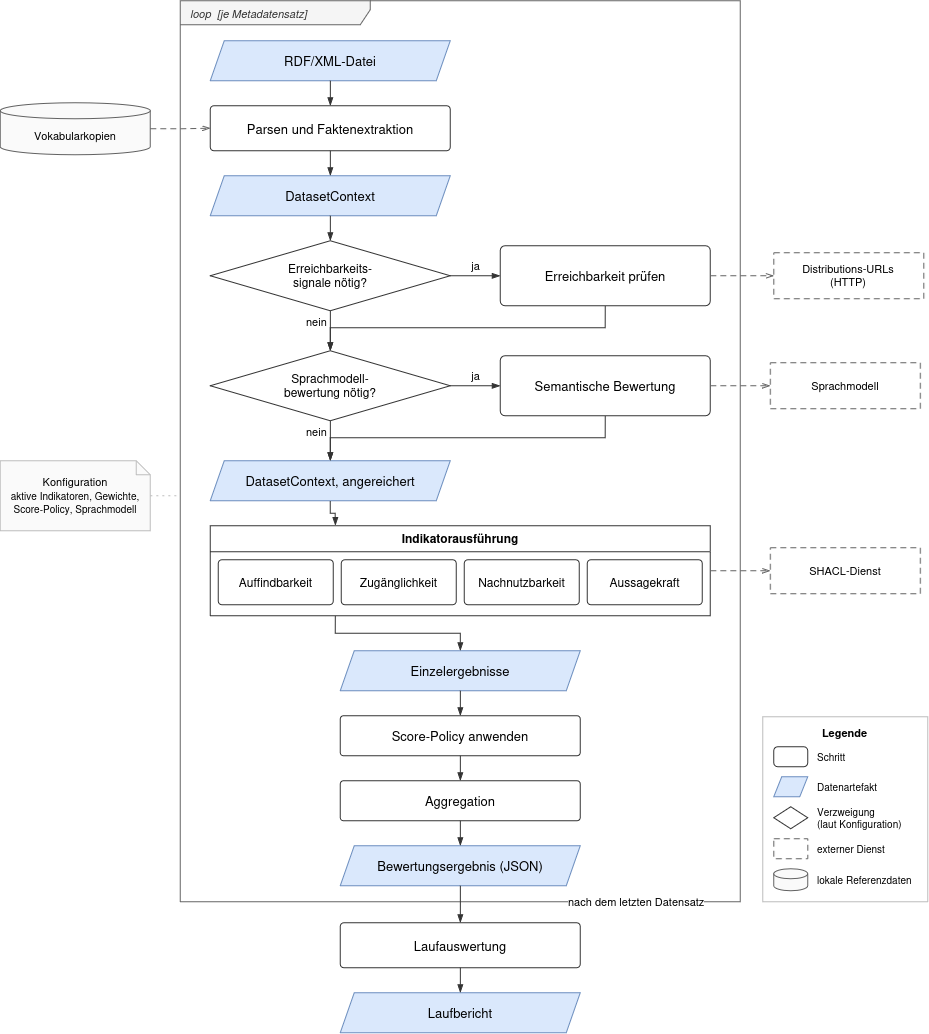
\includegraphics[width=\textwidth]{images/pipeline_prototype.png}
    \captionsetup{justification=centering}
    \caption{Verarbeitungspipeline eines Bewertungslaufs}
    \label{fig:prototyp_architektur}
\end{figure}

Die Verarbeitung beginnt mit dem Einlesen der RDF/XML-Datei. Der Graph wird einmal traversiert und in die Faktenbasis überführt, wobei bereits gegen lokal mitgelieferte Kopien der Referenzlisten vorberechnet wird, ob Themen, Formate, Medientypen und Lizenzen den kontrollierten Vokabularen angehören. Darauf folgen die beiden bedarfsgesteuerten Anreicherungsschritte, die technische Erreichbarkeitsprüfung der Distributionen und die semantische Bewertung der Freitextfelder durch das Sprachmodell. Um sich Netzwerkzugriffe und Sprachmodellaufrufe zu sparen, werden diese nur ausgeführt, wenn nach der aktiven Konfiguration mindestens ein Indikator ihre Ergebnisse tatsächlich konsumiert, andernfalls werden sie übersprungen. Anschließend werden die Indikatoren der vier Qualitätsdimensionen ausgeführt, ihre Einzelergebnisse über die konfigurierte Abbildung von Ergebnisstufen auf Punktwerte vereinheitlicht und zu Dimensions- und Gesamtwerten aggregiert. Das fertige Bewertungsergebnis wird zusammen mit dem Protokoll des Datensatzes abgelegt. Dieser Ablauf wiederholt sich für jede Eingabedatei des Bewertungslaufs. Nach dem letzten Datensatz entstehen zusätzlich laufweite Kennzahlen, Diagramme und Kostenübersichten.

Die Schritte der Pipeline sind nicht unabhängig voneinander lauffähig, sondern über die Faktenbasis sequenziell gekoppelt: Die Bewertung setzt den in der Extraktion aufgebauten Datensatzkontext voraus, und die Anreicherungen können ihre Prüfsignale nur an einen bereits bestehenden Kontext anhängen. Dass sich die Schritte damit ein gemeinsames Datenmodell teilen, ist beabsichtigt und wird in Abschnitt~\ref{sec:extraktion} begründet. Über den eigenen Prozess hinaus greift der Prototyp auf drei externe Dienste zu: Die Endpunkte der Distributionen, das Sprachmodell und auf den SHACL-Validierungsdienst, der aus dem Konformitätsindikator heraus angesprochen wird.

Die Indikatoren registrieren sich bei ihrer Instanziierung selbst in einer zentralen Registrierung, aus der der Bewertungsschritt die auszuführenden Prüfungen bezieht. Ein neuer Indikator besteht damit aus einer einzelnen Klasse, die eine Prüfmethode implementiert, und wird von der Verarbeitungskette automatisch berücksichtigt. Dieses Erweiterungsprinzip setzt die im Bewertungsmodell angelegte Offenheit des Indikatorenkatalogs technisch um.

Der Prototyp ist in Python implementiert und setzt Python~3.12 voraus. Die RDF-Verarbeitung erfolgt mit der Bibliothek rdflib\footnote{\url{https://rdflib.readthedocs.io/}}, die Erreichbarkeitsprüfungen nutzen requests\footnote{\url{https://requests.readthedocs.io/}}. Die strukturierte Ausgabe des Sprachmodells wird über Pydantic\footnote{\url{https://docs.pydantic.dev/}} schemavalidiert, die Anbindung des Modells erfolgt über LangChain\footnote{\url{https://www.langchain.com/}}. Die Konfiguration der Bewertungsläufe wird mit Hydra\footnote{\url{https://hydra.cc/}} verwaltet, die Visualisierungen werden mit matplotlib\footnote{\url{https://matplotlib.org/}} erzeugt. Die exakten Versionsstände aller Abhängigkeiten sind im Quellcode-Repository\footnote{\url{https://github.com/LarsBuergerr/master_thesis_prototype/tree/v3_prototype_freeze}} festgeschrieben. 
% @TODO github link am ende noch updaten falls nötig, und eventuell matplotlib entfernen da die visualisierungen ja dann im frontend erzeugt werden. und das mit den versionständen eventuell weg machen :sob: 

\section{Extraktion und Anreicherung der Metadaten}
\label{sec:extraktion}

Die in der Verarbeitungspipeline aufgebaute Faktenbasis hält je Datensatz alle bewertungsrelevanten Angaben, darunter Titel, Beschreibung, Schlagwörter, Themen sowie Datums- und Frequenzangaben, und für jede Distribution ein eigenes Faktenobjekt mit Format-, Medientyp-, Lizenz- und URL-Angaben. Häufig benötigte abgeleitete Größen wie die Anzahl der Distributionen mit Download-URL werden als berechnete Eigenschaften bereitgestellt.

Ihre Einführung als eigene Zwischenstufe zwischen RDF-Graph und Indikatoren ist eine bewusste Entwurfsentscheidung. Sie stellt erstens Konsistenz sicher, da alle Indikatoren über dieselben, an genau einer Stelle extrahierten Fakten urteilen und Interpretationsfragen der RDF-Struktur nicht je Indikator unterschiedlich beantwortet werden können. Desweiteren wird redundante Arbeit vermieden, da der Graph nur einmal traversiert wird. Zudem wird die Prüflogik vom Datenmodell entkoppelt, denn die Indikatoren operieren auf typisierten Werten und enthalten keine RDF-spezifische Logik, was ihre Implementierung und Erweiterung wesentlich vereinfacht.

\begin{listing}[H]
\begin{minted}
[
frame=lines,
framesep=2mm,
baselinestretch=1.2,
fontsize=\footnotesize
]
{python}
DatasetContext(
    titles=["Radverkehrsnetz Brandenburg"],
    keywords=["Radverkehr", "Radwege", "Infrastruktur"],
    themes=[".../data-theme/TRAN"],
    themes_in_vocab=[True],
    distributions=[
        DistributionContext(
            download_url="https://geoportal.example.de/radnetz.csv",
            formats=[".../file-type/CSV"],
            formats_in_vocab=[True],
            licenses_open=[True],
            probe=DistributionProbe(          # technische Anreicherung
                fetched=True,
                download_status_code=200,
                coalesced_mime="text/csv",
                machine_readable_tier="high",
                is_non_proprietary=True,
            ),
        ),
    ],
    semantic_assessment=ExpressivenessAssessment(  # semantische Anreicherung
        title_quality=ExpressivenessCriterion(
            findings=["Titel nennt Thema und Raumbezug", ...],
            reasoning="...",
            applicable=True,
            score=0.8,
        ),
        ...,  # weitere Kriterien
    ),
)
\end{minted}
\caption{Exemplarisch gefüllte Faktenbasis nach beiden Anreicherungsstufen, gekürzt}
\label{lst:dataset_context}
\end{listing}

Listing~\ref{lst:dataset_context} zeigt exemplarisch eine gekürzte Faktenbasis nach Abschluss beider Anreicherungsstufen. Neben den extrahierten Rohwerten sind die vorberechneten Vokabularprüfungen wie \texttt{themes\_in\_vocab} sichtbar sowie die angehängten Prüfsignale: Das Ergebnis der Erreichbarkeitsprüfung liegt je Distribution im Feld \texttt{probe}, die semantische Bewertung datensatzweit im Feld \texttt{semantic\_assessment}.


Prüfungen gegen kontrollierte Vokabulare stützen sich auf lokal mitgelieferte Kopien der Referenzlisten, die einmalig beim Start geladen werden. Dazu gehören die Vokabulare des Publications Office der Europäischen Union für Themen, Dateitypen und Aktualisierungsfrequenzen\footnote{\url{https://op.europa.eu/en/web/eu-vocabularies/authority-tables}}, das Medientypregister der IANA\footnote{\url{https://www.iana.org/assignments/media-types/}} sowie die Lizenzliste, die IDs der Datenbereitsteller und das Schlüsselverzeichnis der politischen Geokodierung aus DCAT-AP.de \cite{DCATAPDEImplRules2}. Die lokale Bündelung macht die Vokabularprüfungen deterministisch und unabhängig von der Verfügbarkeit externer Dienste.

Die technische Anreicherung prüft die Erreichbarkeit der in den Distributionen angegebenen Zugriffs- und Download-URLs. Jede eindeutige URL wird höchstens einmal je Bewertungslauf angefragt, zunächst über eine HEAD-Anfrage und ergänzend über eine GET-Anfrage mit abgebrochenem Inhaltsbezug: Die Verbindung wird unmittelbar nach Eintreffen der Antwort-Header geschlossen, ohne den Antwortkörper zu lesen. Erfasst werden unter anderem der HTTP-Statuscode, der zurückgelieferte Medientyp und die Fehlerklasse fehlgeschlagener Anfragen. Die Ergebnisse werden als Prüfsignale an die Faktenbasis angehängt und von allen konsumierenden Indikatoren gemeinsam genutzt.

Die semantische Anreicherung erzeugt bei aktivierten Aussagekraftsindikatoren eine strukturierte Bewertung der Freitextfelder und hängt sie ebenfalls an die Faktenbasis an. Sie folgt demselben Prinzip wie die technische Anreicherung: Die Bewertung wird genau einmal je Datensatz erstellt und anschließend von allen sechs Aussagekraftsindikatoren gemeinsam ausgewertet.

\section{Implementierung der Einzelindikatoren}
\label{sec:einzelindikatoren}

\begin{wrapfigure}{r}{0.45\textwidth}
\vspace{-\baselineskip}
\begin{minted}
[
frame=lines,
framesep=2mm,
baselinestretch=1.2,
fontsize=\small
]
{python}
class ThemeIndicator(Indicator):
  def validate(self, context):
    if not context.themes:
      return self.result(FAIL)
    if all(context.themes_in_vocab):
      return self.result(PASS)
    return self.result(PARTIAL)
\end{minted}
\captionof{listing}{Implementierungsmuster eines ternären Indikators, vereinfacht}
\label{lst:indicator_anatomy}
\end{wrapfigure}

Alle Indikatoren folgen derselben Implementierungsstruktur. Ein Indikator ist eine Klasse mit einer einzelnen Prüfmethode, die die Faktenbasis liest und ein Ergebnisobjekt zurückgibt. Das Ergebnisobjekt enthält die Ergebnisstufe, den Erfüllungsgrad, eine deutsch- und englischsprachige Ergebnismeldung sowie ein Detailobjekt mit den geprüften Werten, aus dem sich das Urteil im Reporting nachvollziehen lässt. Listing~\ref{lst:indicator_anatomy} zeigt das Muster in vereinfachter Form am Beispiel der Themenkategorie. Da die Faktenbasis die Vokabularzugehörigkeit bereits vorberechnet bereitstellt, reduziert sich die Prüflogik der meisten formalen Indikatoren auf wenige Fallunterscheidungen.

Die folgenden Abschnitte dokumentieren je Dimension die gemeinsame Prüfmechanik und die konkreten Prüfregeln einschließlich der gewählten Schwellwerte. Die konzeptionelle Herleitung der Indikatoren wird nicht wiederholt, referenziert wird ausschließlich über die Kürzel aus Kapitel~4.

\subsection{Abbildung des konzeptionellen Modells auf implementierte Indikatoren}

Da das konzeptionelle Modell bereits auf operationalisierbare Indikatoren zugeschnitten ist, bilden die implementierten Indikatoren die Konzept-Kürzel eins zu eins ab. Insgesamt sind 27 Indikatoren umgesetzt. Tabelle~\ref{tab:impl_mapping} führt sie mit ihrem Namen und ihrem Bezeichner in der Implementierung auf. Diese Bezeichner erscheinen in den Bewertungsergebnissen, den Reports und den Auswertungen der Evaluation. Die Tabelle dient damit als durchgängige Referenz zwischen Konzept, Quellcode und Ergebnisdarstellung.

\begin{table}[H]
\centering
\scriptsize
\renewcommand{\arraystretch}{1.2}
\rowcolors{1}{white}{white}
\begin{tabular}{p{0.06\textwidth} >{\raggedright\arraybackslash}p{0.42\textwidth} >{\raggedright\arraybackslash}p{0.38\textwidth}}
\hline
\textbf{Kürzel} & \textbf{Indikatorname} & \textbf{Indikator-Bezeichner} \\
\hline
A1 & Schlagwortumfang in angemessenem Bereich & \texttt{find\_keywords\_count} \\
\hline
A2 & Themenkategorie aus kontrolliertem Vokabular & \texttt{find\_theme\_valid} \\
\hline
A3 & Räumliche Geometrieangabe vorhanden & \texttt{find\_locn\_geometry} \\
\hline
A4 & Politische Geokodierung aus DCAT-AP.de-Vokabular & \texttt{find\_political\_geocoding} \\
\hline
A5 & Ebene der politischen Geokodierung aus Vokabular & \texttt{find\_geocoding\_level} \\
\hline
A6 & Zeitliche Abdeckung mit valider Datumsangabe & \texttt{find\_temporal\_coverage} \\
\hline
A7 & Veröffentlichungsdatum valide typisiert & \texttt{find\_issued\_datetime} \\
\hline
A8 & Änderungsdatum valide typisiert & \texttt{find\_modified\_datetime} \\
\hline
Z1 & Download-URL angegeben & \texttt{acc\_download\_url} \\
\hline
Z2 & Formatangabe aus kontrolliertem Vokabular & \texttt{acc\_format} \\
\hline
Z3 & Medientyp als IANA-Medientyp & \texttt{acc\_media\_type} \\
\hline
Z4 & Nicht-proprietäres Format & \texttt{acc\_format\_non\_proprietary} \\
\hline
Z5 & Download-URL technisch erreichbar & \texttt{acc\_download\_url\_response} \\
\hline
Z6 & Access-URL technisch erreichbar & \texttt{acc\_access\_url\_response} \\
\hline
Z7 & Maschinenlesbarer Zugriffsweg (abgestuft) & \texttt{acc\_machine\_readable\_access} \\
\hline
N1 & Freie Lizenz aus DCAT-AP.de-Lizenzliste & \texttt{reuse\_license} \\
\hline
N2 & Herausgeber als strukturierter Agent mit Namen & \texttt{reuse\_publisher} \\
\hline
N3 & Kontaktpunkt mit nutzbarer E-Mail oder URL & \texttt{reuse\_contact} \\
\hline
N4 & Geplante Verfügbarkeit aus kontrolliertem Vokabular & \texttt{reuse\_availability} \\
\hline
N5 & ContributorID aus Contributor-Vokabular & \texttt{reuse\_contributor\_id} \\
\hline
N6 & DCAT-AP.de-Konformität (SHACL-Validierung) & \texttt{reuse\_dcat\_ap\_de\_compliance} \\
\hline
S1 & Aussagekraft des Titels & \texttt{expr\_title\_quality} \\
\hline
S2 & Aussagekraft der Beschreibung & \texttt{expr\_description\_quality} \\
\hline
S3 & Kohärenz von Titel und Beschreibung & \texttt{expr\_title\_description\_coherence} \\
\hline
S4 & Qualität der Schlagwörter & \texttt{expr\_keyword\_quality} \\
\hline
S5 & Thematische Konsistenz & \texttt{expr\_thematic\_consistency} \\
\hline
S6 & Kontextuelle Qualifizierer & \texttt{expr\_contextual\_qualifiers} \\
\hline
\end{tabular}
\caption{Konzept-Kürzel, Indikatorname und Bezeichner in der Implementierung}
\label{tab:impl_mapping}
\end{table}

\subsection{Auffindbarkeitsindikatoren}

Die Auffindbarkeitsindikatoren prüfen datensatzweite Angaben direkt auf der Faktenbasis und benötigen weder Netzwerkzugriffe noch das Sprachmodell. Mit Ausnahme der beiden Datumsindikatoren A7 (Veröffentlichungsdatum) und A8 (Änderungsdatum) sind alle ternär. Die beiden Datumsindikatoren messen graduell den Anteil der vorhandenen Datumswerte mit validem \texttt{xsd:date}- oder \texttt{xsd:dateTime}-Typ, wobei Angaben auf Datensatz- und Distributionsebene gemeinsam betrachtet werden. Fehlt die jeweilige Angabe vollständig, gilt der Indikator als nicht erfüllt. Tabelle~\ref{tab:impl_findability} fasst die Prüfregeln zusammen.

\begin{table}[H]
\centering
\scriptsize
\renewcommand{\arraystretch}{1.2}
\rowcolors{1}{white}{white}
\begin{tabular}{p{0.06\textwidth} >{\raggedright\arraybackslash}p{0.84\textwidth}}
\hline
\textbf{Kürzel} & \textbf{Prüfregel} \\
\hline
A1 & Erfüllt bei 3 bis 15 Schlagwörtern, teilweise erfüllt bei 1 bis 2 oder 16 bis 25, nicht erfüllt bei 0 oder mehr als 25 \\
\hline
A2 & Erfüllt, wenn alle Themenkategorien aus dem EU-Vokabular stammen, teilweise erfüllt, wenn nur ein Teil daraus stammt, nicht erfüllt ohne Themenkategorie \\
\hline
A3 & Erfüllt, wenn eine Geometrieangabe vorhanden ist, sonst nicht erfüllt \\
\hline
A4 & Erfüllt, wenn die Geokodierungs-URI im DCAT-AP.de-Vokabular liegt, teilweise erfüllt bei einer Angabe außerhalb des Vokabulars oder bei ausschließlicher Nutzung des Rückfallwerts \texttt{locn:adminUnitL2}, nicht erfüllt ohne Angabe \\
\hline
A5 & Erfüllt, wenn die Ebenenangabe im Vokabular liegt, teilweise erfüllt bei einer Angabe außerhalb des Vokabulars, nicht erfüllt ohne Angabe \\
\hline
A6 & Erfüllt, wenn ein valider Start- oder Endwert der zeitlichen Abdeckung vorliegt, sonst nicht erfüllt \\
\hline
A7 & Graduell: Anteil der vorhandenen \texttt{dct:issued}-Werte mit validem Datumstyp, nicht erfüllt ohne Angabe \\
\hline
A8 & Graduell: Anteil der vorhandenen \texttt{dct:modified}-Werte mit validem Datumstyp, nicht erfüllt ohne Angabe \\
\hline
\end{tabular}
\caption{Prüfregeln der Auffindbarkeitsindikatoren}
\label{tab:impl_findability}
\end{table}

Die Schlagwortspanne von 3 bis 15 ist direkt aus der Handreichung zur Verbesserung der Metadatenqualität des open bydata competence center übernommen, die für einen Datensatz mindestens drei relevante Schlagwörter empfiehlt und je nach Dateninhalt maximal 15 Begriffe als ausreichend ansieht \cite{bydata2025handreichung}. Werte innerhalb dieser Spanne gelten als erfüllt, ein bis zwei oder 16 bis 25 Schlagwörter als Teilerfüllung und darüber hinausgehende Werte als nicht erfüllt. Die Abstufung bei der politischen Geokodierung folgt der Konventionstreue. Die dedizierte Eigenschaft \texttt{dcatde:politicalGeocodingURI} ist gemäß Konvention 08 des DCAT-AP.de-Konventionenhandbuchs der vorgesehene Weg, den verwaltungspolitischen Geobezug als URI aus dem zugehörigen kontrollierten Vokabular auszudrücken \cite{DCATAPDEImplRules2}. Der Rückfall auf \texttt{locn:adminUnitL2} transportiert dieselbe Information in schwächer standardisierter Form und wird daher nur als Teilerfüllung gewertet.

\subsection{Zugänglichkeitsindikatoren}

Alle Zugänglichkeitsindikatoren messen graduell je Distribution und mitteln die Einzelbeiträge zum Datensatzergebnis. Listing~\ref{lst:graded_scoring} zeigt das gemeinsame Bewertungsmuster in vereinfachter Form. Die Indikatoren unterscheiden sich ausschließlich in der Beitragsfunktion, die einer einzelnen Distribution ihren Wert zuweist. Tabelle~\ref{tab:impl_accessibility} definiert diese Beitragsfunktionen. Die Erreichbarkeitsprüfungen stützen sich auf die zuvor erhobenen Prüfsignale und werten einen HTTP-Statuscode unter 400 als erreichbar. 
% @TODO eventuell noch adden dass das generierte Label / Erfüllungsgrad keinen Einfluss auf die Berechnung hat sondern nur als Reporting dient. Bei allen graduellen Indikatoren wird der Raw Score aus den Beiträgen berechnet.

\begin{listing}[H]
\begin{minted}
[
frame=lines,
framesep=2mm,
baselinestretch=1.2,
fontsize=\small
]
{python}
def score(distributions, contribution) -> float:
    if not distributions:
        return NOT_APPLICABLE
    return mean(contribution(d) for d in distributions)

# Beitragsfunktion Z5 (Erreichbarkeit der Download-URL):
def contribution(dist) -> float:
    if dist.probe.download_status_code < 400:
        return 1.0
    return -0.5  # Malus
\end{minted}
\caption{Gemeinsames Bewertungsmuster der distributionsbezogenen Indikatoren, vereinfacht}
\label{lst:graded_scoring}
\end{listing}

\begin{table}[H]
\centering
\scriptsize
\renewcommand{\arraystretch}{1.2}
\rowcolors{1}{white}{white}
\begin{tabular}{p{0.06\textwidth} >{\raggedright\arraybackslash}p{0.84\textwidth}}
\hline
\textbf{Kürzel} & \textbf{Beitrag je Distribution} \\
\hline
Z1 & 1 bei vorhandener Download-URL, sonst 0 \\
\hline
Z2 & 1 bei Formatangabe aus dem EU-Dateitypvokabular, sonst 0 \\
\hline
Z3 & 1 bei Medientyp als IANA-URI aus dem Register, sonst 0 \\
\hline
Z4 & 1 bei nicht-proprietärem Format laut EU-Dateitypvokabular, sonst 0 \\
\hline
Z5 & 1 bei erreichbarer Download-URL, $-$0,5 bei nicht erreichbarer \\
\hline
Z6 & 1 bei erreichbarer Access-URL, $-$0,5 bei nicht erreichbarer \\
\hline
Z7 & 1 bei Stufe \textit{high}, 0,5 bei Stufe \textit{mid}, 0 bei Stufe \textit{none} \\
\hline
\end{tabular}
\caption{Beitragsfunktionen der Zugänglichkeitsindikatoren}
\label{tab:impl_accessibility}
\end{table}

Die Stufenzuordnung von Z7 (maschinenlesbarer Zugriffsweg) orientiert sich an der Klassifikation maschinenlesbarer Dateitypen der Data Quality Guidelines von data.europa.eu \cite{dataeuropa_dqguidelines}. Deren Tabelle unterscheidet drei Grade der Maschinenlesbarkeit, die unmittelbar auf die drei Stufen des Indikators abgebildet werden. Vollständig maschinenlesbare Formate wie CSV, JSON, XML oder RDF sowie deklarierte Datenservice-Endpunkte werden als \textit{high} eingestuft, überwiegend maschinenlesbare Formate wie XLSX, ODS, XLS, HTML oder reine Textdateien als \textit{mid} und nicht maschinenlesbare Auslieferungen wie PDF, Office-Dokumente oder Bildformate als \textit{none}. Da die zugrunde liegende Klassifikation geospezifische Datentypen nicht berücksichtigt, wurde sie um solche Formate ergänzt, etwa Shapefile, die entsprechend ihrer Maschinenlesbarkeit eingeordnet werden. Anders als die Erreichbarkeitsprüfungen Z5 und Z6 wendet Z7 das Malus-Prinzip nicht an; die Stufe \textit{none} geht mit 0 in die Distributionsmittelung ein, da eine nicht maschinenlesbare Distribution keine Verfügbarkeit vortäuscht, sondern liefert, was sie deklariert.

\subsection{Nachnutzbarkeitsindikatoren}

Die Nachnutzbarkeitsindikatoren kombinieren beide Messformen. N1 (freie Lizenz) und N4 (geplante Verfügbarkeit) messen graduell je Distribution nach dem Muster aus Listing~\ref{lst:graded_scoring}, die übrigen Indikatoren prüfen ternär auf Datensatzebene. Tabelle~\ref{tab:impl_reusability} fasst die Prüfregeln zusammen.

\begin{table}[H]
\centering
\scriptsize
\renewcommand{\arraystretch}{1.2}
\rowcolors{1}{white}{white}
\begin{tabular}{p{0.06\textwidth} >{\raggedright\arraybackslash}p{0.84\textwidth}}
\hline
\textbf{Kürzel} & \textbf{Prüfregel} \\
\hline
N1 & Graduell je Distribution: 1 bei freier Lizenz aus der DCAT-AP.de-Lizenzliste, $-$0,5 bei eingeschränkter, unbekannter oder fehlender Lizenz \\
\hline
N2 & Erfüllt, wenn der Herausgeber als \texttt{foaf:Agent} typisiert ist und einen \texttt{foaf:name} trägt, teilweise erfüllt bei nur einem der beiden Merkmale, sonst nicht erfüllt \\
\hline
N3 & Erfüllt, wenn der Kontaktpunkt eine valide E-Mail-Adresse oder URL enthält, teilweise erfüllt bei Kontaktpunkt ohne nutzbaren Kanal, nicht erfüllt ohne Kontaktpunkt \\
\hline
N4 & Graduell je Distribution: 1 bei Verfügbarkeitsangabe aus dem Planned-Availability-Vokabular, sonst 0 \\
\hline
N5 & Erfüllt, wenn genau eine \texttt{dcatde:contributorID} als IRI aus dem Contributor-Vokabular vorliegt, sonst nicht erfüllt \\
\hline
N6 & Erfüllt bei null SHACL-Verletzungen gegen das DCAT-AP.de-Regelwerk, nicht erfüllt bei mindestens einer Verletzung \\
\hline
\end{tabular}
\caption{Prüfregeln der Nachnutzbarkeitsindikatoren}
\label{tab:impl_reusability}
\end{table}

Der Lizenzindikator N1 wendet als einziger Indikator dieser Dimension das Malus-Prinzip an. Die Gleichbehandlung von eingeschränkten, unbekannten und fehlenden Lizenzen folgt der Nutzendenperspektive, denn in allen drei Fällen ist die Rechtslage ungeklärt und die Nachnutzung damit gleichermaßen blockiert.

Die Konformitätsprüfung N6 validiert den Metadatensatz nicht mit einer lokalen Kopie der SHACL-Shapes, sondern über den öffentlich betriebenen SHACL-Validierungsdienst des Interoperability Test Bed der Europäischen Kommission\footnote{Weboberfläche des Dienstes: \url{https://www.itb.ec.europa.eu/shacl/dcat-ap.de/upload}. Der Prototyp spricht die zugehörige REST-Schnittstelle unter \texttt{/shacl/dcat-ap.de/api/validate} per POST an. Ein direkter Aufruf dieser Adresse im Browser beantwortet der Dienst erwartungsgemäß mit \texttt{405 Method Not Allowed}.}. Dadurch wird stets gegen das offiziell gepflegte DCAT-AP.de-Regelwerk geprüft und die Urteile bleiben deckungsgleich mit dem Referenzvalidator, ohne dass der Prototyp eine eigene Regelwerkskopie aktuell halten muss. Geprüft wird gegen das Profil in der Version~2.0. Diese Version bildet ein vollständig abgeschlossenes Profil, das neben der Spezifikation auch ein zugehöriges Konventionenhandbuch bereitstellt \cite{DCATAPDESpec2, DCATAPDEImplRules2} und damit die Grundlage des in Kapitel~4 abgeleiteten Bewertungsmodells bildet. Die im Dezember 2024 veröffentlichte Version~3.0 wird bewusst nicht verwendet, da für sie kein geschlossenes Konventionenhandbuch mehr vorgesehen ist; die Konventionen werden stattdessen in die Spezifikation überführt, in Guidelines umgewandelt oder gestrichen, wobei entsprechende Guidelines bislang nicht vorliegen \cite{DCATAPDESpec3}. Die Bewertung ist binär, da Standardkonformität keine sinnvolle Teilerfüllung kennt. Als einziger Indikator hängt N6 von der Verfügbarkeit eines externen Dienstes ab. Ist der Dienst nicht erreichbar, wird der Indikator als Fehler ausgewiesen.

\section{LLM-gestützte Bewertung der Aussagekraft}
\label{sec:llm_aussagekraft}

Die Aussagekraft ist die einzige Qualitätsdimension, die sich nicht regelbasiert bestimmen lässt. Kapitel~4 hat begründet, dass ihre Kriterien ein sprachverstehendes Verfahren als Messinstrument erfordern. Der vorliegende Abschnitt beschreibt, wie dieses Instrument im Prototyp umgesetzt ist, und behandelt damit den zentralen Baustein der dritten Teilfrage dieser Arbeit, welche ergänzenden kontext- und semantikbezogenen Prüfungen das formale Qualitätsmodell sinnvoll erweitern können, ohne die Nachvollziehbarkeit und Verlässlichkeit des Scorings zu gefährden (vgl. Abschnitt~\ref{sec:forschungsfragen}). Bewertet werden dabei ausschließlich Metadaten offener Verwaltungsdaten, die ohnehin frei im Netz veröffentlicht sind. Ihre Übergabe an ein externes Sprachmodell wirft daher keine Fragen des Datenschutzes oder der Vertraulichkeit auf.

\subsection{Ein-Aufruf-Architektur}

Für das Sprachmodell verfolgt der Prototyp eine Ein-Aufruf-Architektur. 
Statt die sechs Kriterien einzeln abzufragen, wird der gesamte Datensatz in einem einzigen Aufruf bewertet.
Das Ergebnis wird an die Faktenbasis angehängt, und jeder Indikator liest daraus seinen Teil. 
Damit folgt die semantische Anreicherung dem gleichen Muster wie die technische Erreichbarkeitsprüfung, bei der die geteilte Ressource einmal berechnet und von allen Konsumenten gemeinsam genutzt wird. Zum einen werden durch dieses Vorgehen Kosten reduziert, da statt sechs Aufrufen nur einer je Datensatz anfällt. Zum anderen erhöht der gemeinsame Aufruf die Konsistenz der Bewertung. Alle sechs Kriterien gehen aus derselben ganzheitlichen Betrachtung des Datensatzes hervor und beruhen damit auf einem einheitlichen Verständnis der Metadaten. Widersprüche zwischen den Einzelurteilen, wie sie bei sechs voneinander unabhängigen Aufrufen entstehen könnten, werden dadurch unwahrscheinlich. Schlägt der Aufruf fehl oder ist kein Modell konfiguriert, bleibt die Bewertung leer und die Aussagekraftsindikatoren melden \textit{nicht anwendbar}, statt den Bewertungslauf abzubrechen.

\subsection{Strukturierte Ausgabe}

Die Ausgabe des Sprachmodells ist kein Freitext, sondern ein schemavalidiertes Objekt. Das Schema wird mit Pydantic definiert und dem Modell als verbindliche Ausgabestruktur vorgegeben, sodass die Antwort nicht nachträglich geparst werden muss, sondern typgeprüft vorliegt. Jedes der sechs Kriterien entspricht einem Feld des Schemas und ist damit eins zu eins einem Aussagekraftsindikator (S1 bis S6) zugeordnet. Ein einzelnes Kriterium besteht aus vier Feldern in fester Reihenfolge: zunächst ein bis drei beobachtbare \texttt{findings}, daraus abgeleitet eine kurze \texttt{reasoning}-Begründung, anschließend ein \texttt{applicable}-Flag und erst zuletzt ein kontinuierlicher \texttt{score} zwischen 0 und 1. Diese Reihenfolge erzwingt, dass das Modell zuerst die beobachtbare Evidenz benennt und sein Urteil daraus herleitet, bevor es einen Zahlenwert festlegt. Listing~\ref{lst:expr_schema} zeigt das Schema in vereinfachter Form.

\begin{listing}[H]
\begin{minted}
[
frame=lines,
framesep=2mm,
baselinestretch=1.2,
fontsize=\small
]
{python}
class ExpressivenessCriterion(BaseModel):
    findings: list[str] = Field(
        default_factory=list,
        max_length=3,
        description=(
            "Zuerst ausfüllen: 1-3 konkrete, beobachtbare Stärken/Schwächen für "
            "dieses Kriterium."
        ),
    )
    reasoning: str = Field(...)
    applicable: bool = Field(...)
    score: float = Field(...)

    @property
    def status(self) -> str:      # Label, aus score abgeleitet
        if not self.applicable:
            return "not_applicable"
        if self.score >= 0.8:
            return "pass"
        if self.score >= 0.5:
            return "partial"
        return "fail"

class ExpressivenessAssessment(BaseModel):
    title_quality: ExpressivenessCriterion
    description_quality: ExpressivenessCriterion
    title_description_coherence: ExpressivenessCriterion
    keyword_quality: ExpressivenessCriterion
    thematic_consistency: ExpressivenessCriterion
    contextual_qualifiers: ExpressivenessCriterion
\end{minted}
\caption{Pydantic-Schema der Aussagekraftsbewertung, vereinfacht}
\label{lst:expr_schema}
\end{listing}

Zwei Eigenschaften des Schemas sind für die Nachvollziehbarkeit entscheidend. Erstens wird die diskrete Ergebnisstufe nicht vom Modell erfragt, sondern deterministisch aus dem \texttt{score} abgeleitet. Das Modell liefert ausschließlich den kontinuierlichen Wert samt Begründung, sodass Stufe und Wert einander nicht widersprechen können. Zweitens setzt das \texttt{applicable}-Flag die im Messmodell vorgesehene Nicht-Anwendbarkeit um: Ein Kriterium, das der Datentyp nicht erfordert, etwa ein kontextueller Qualifizierer bei einem statischen Datensatz, wird neutral übersprungen statt abgewertet. Jeder Aussagekraftswert ist damit auf benennbare Befunde und eine Begründung zurückführbar.

\subsection{Eingabe und Prompt}

Der Aufruf trennt Systemanweisung und Nutzereingabe. Die Systemanweisung legt die Rolle des Modells als Auditor ausschließlich für die Aussagekraft fest und grenzt technische Zugänglichkeit, Lizenzierung und Auffindbarkeit ausdrücklich aus. Sie enthält die schrittweise Vorgehensweise je Kriterium, die aus dem DCAT-AP.de-Konventionenhandbuch v2.0 (Kapitel 1.7 und 3.4) sowie der Handreichung zur Verbesserung der Metadatenqualität abgeleiteten Bewertungsregeln \cite{DCATAPDEImplRules2, bydata2025handreichung} und eine Ankerskala, die Wertebereiche verbal an Qualitätsniveaus bindet. Die Nutzereingabe enthält die zu bewertenden Metadaten. Übergeben wird dabei nicht der vollständige RDF-Graph, sondern die bereits in Abschnitt~\ref{sec:extraktion} aufgebaute, auf die bewertungsrelevanten Freitext- und Klassifikationsfelder reduzierte Sicht der Faktenbasis. Das begrenzt den Tokenverbrauch und fokussiert das Modell auf den Bewertungsgegenstand. Listing~\ref{lst:expr_call} zeigt den Aufbau des Aufrufs.

\begin{listing}[H]
\begin{minted}{python}
def assess(context, llm) -> ExpressivenessAssessment:
    payload = context.to_agent_json()   # gekuerzte Faktenbasis
    messages = [
        ("system", SYSTEM_PROMPT),       # Rolle, Rubrik, Ankerskala
        ("human", USER_PROMPT.format(context=payload)),
    ]
    # Schema als verbindliche Ausgabestruktur erzwingen
    structured = llm.with_structured_output(ExpressivenessAssessment)
    return structured.invoke(messages)
\end{minted}
\caption{Aufbau des Sprachmodellaufrufs mit gekürztem Kontext und erzwungenem Schema, vereinfacht}
\label{lst:expr_call}
\end{listing}

Zwei Vorkehrungen erhöhen die Robustheit der Bewertung. Zum einen wird das Modell angewiesen, die reine Feldpräsenz nicht als Qualität zu werten, sondern generische, kryptische oder widersprüchliche Angaben trotz Vorhandensein abzuwerten. Zum anderen wird der Metadateninhalt durch Trennmarken abgegrenzt und ausdrücklich als reiner Bewertungsgegenstand deklariert, den das Modell niemals als Anweisung behandeln darf. Damit wird verhindert, dass in Metadatenfeldern eingebetteter Text die Bewertung manipuliert. Der vollständige Wortlaut von System- und Nutzeranweisung sowie die Pydantic-Schemata sind im Anhang \ref{app:prompts_semantische_anreicherung} dokumentiert. % @TODO evenutell prompt im anhang bei potenziellen Änderungen noch einmal updaten.

\subsection{Determinismus und Konfiguration}

Der Aufruf erfolgt mit einer Temperatur von 0. Für ein Bewertungsinstrument ist Reproduzierbarkeit wichtiger als sprachliche Variation, und eine Temperatur von 0 maximiert die Bestimmtheit der Ausgabe, sodass identische Eingaben möglichst identische Bewertungen ergeben. Das stützt unmittelbar das Nachvollziehbarkeitsziel des Prototyps und die Anforderung einer reproduzierbaren Evaluation. Die Ausgabelänge ist auf 10.000 Tokens begrenzt. Diese Grenze lässt der strukturierten Antwort ausreichend Raum, sodass sie nicht abgeschnitten wird, und deckelt zugleich die Kosten eines einzelnen Aufrufs. Als Modell wird Claude Sonnet~4.5 verwendet, angebunden über den Dienst OpenRouter. 

%@TODO eventuell noch ein satz verschwenden dass verglichen wurde gegen gpt4.5 und opus

\section{Scoring-, Gewichtungs- und Aggregationslogik}

Wie in Sektion \ref{sec:wang_strong_definition_quality} erläutert, ist Datenqualität kein eindimensionales Konstrukt, sondern setzt sich aus mehreren, getrennt zu messenden Dimensionen zusammen \cite{wang1996beyond}. Das Bewertungsmodell folgt dieser Auffassung mit einer zweistufigen Aggregation. Die Indikatorergebnisse werden zunächst je Dimension zu einem Dimensionswert verdichtet, und die Dimensionswerte anschließend zu einem Gesamtscore. Beide Stufen sind gewichtete Mittelwerte, deren Gewichte konfigurierbar sind und nicht im Quellcode festgelegt werden. Die folgenden Angaben beschreiben die in der Evaluation verwendete Konfiguration.

\subsection{Punktevergabe je Indikator}

Ternäre Indikatoren werden über ihre Ergebnisstufe in einen Punktwert überführt. Ein erfülltes Kriterium erhält den Wert 1,0, ein teilweise erfülltes 0,5 und ein nicht erfülltes 0,0. Der Wert 0,5 für die Teilerfüllung entspricht dem Mittelpunkt der Skala und behandelt die Zwischenstufe damit als genau halb erfülltes Kriterium, ohne eine Richtung zu bevorzugen. Graduelle Indikatoren tragen unmittelbar ihren kontinuierlichen Erfüllungsgrad bei. Ihre Ergebnisstufe hat, wie in Abschnitt~\ref{sec:einzelindikatoren} beschrieben, keinen Einfluss auf die Punktevergabe. Innerhalb der graduellen Indikatoren wirkt der Malus: Eine nicht erreichbare URL und eine eingeschränkte, unbekannte oder fehlende Lizenz gehen mit $-$0,5 statt mit 0 in die Distributionsmittelung ein. Als \textit{nicht anwendbar} oder als Fehler ausgewiesene Indikatoren werden neutral behandelt und gehen weder in den Zähler noch in den Nenner der Aggregation ein.

Die konkreten Punktwerte sind normative Setzungen. Ein empirisch optimaler Wert existiert für solche Größen nicht, und auch etablierte Bewertungsmodelle legen ihre Punktwerte per Konvention fest, wie die Punkteverteilung der MQA zeigt (vgl. Tabelle~\ref{tab:mqa_metrics_weights}) \cite{data_europa}. Die Literatur zu zusammengesetzten Indikatoren behandelt die Gewichts- und Punktwahl entsprechend als transparent zu dokumentierende Entwurfsentscheidung, die sich auf Experten- und Konstrukteursurteile stützt \cite{nardo2008handbook}. Kubler et al. zeigen mit ihrem AHP-basierten Ansatz zudem, dass Qualitätsgewichte grundsätzlich präferenzabhängig sind und je nach Stakeholderperspektive unterschiedlich ausfallen \cite{kubler2018comparison}. Maßgeblich für das Modell sind daher weniger die Absolutwerte als die durch sie ausgedrückten Relationen: Teilerfüllung zählt halb, und ein irreführender Defekt wiegt schwerer als eine fehlende Angabe. Für die Malus-Höhe von $-$0,5 bedeutet das konkret, dass zwei defekte Distributionen den Beitrag einer funktionierenden vollständig aufheben.
% @TODO(eigen): Begründung der Malus-Höhe ggf. um Interview-Belegstellen (data-breaking) erweitern, sobald die Argumentation für Kapitel 6 steht

\subsection{Aggregation zum Gesamtscore}

Der Wert einer Dimension $d$ ergibt sich als gewichteter Mittelwert über die Menge $A_d$ ihrer aktiven und anwendbaren Indikatoren, wobei $p_i$ den Punktwert und $w_i$ das Gewicht eines Indikators bezeichnet. Da der Malus einzelne Beiträge negativ werden lässt, wird der Dimensionswert bei 0 nach unten begrenzt:

\begin{equation}
s_d = \max\left(0,\ \frac{\sum_{i \in A_d} w_i \cdot p_i}{\sum_{i \in A_d} w_i}\right)
\label{eq:dimension_score}
\end{equation}

Der Gesamtscore $S$ ist der mit den Dimensionsgewichten $W_d$ gewichtete Mittelwert der Dimensionswerte:

\begin{equation}
S = \frac{\sum_{d} W_d \cdot s_d}{\sum_{d} W_d}
\label{eq:overall_score}
\end{equation}

Aus dem Gesamtscore wird abschließend eine Gesamtnote abgeleitet, die das Ergebnis für das Reporting verdichtet. Ab 0,9 wird die Note A vergeben, ab 0,75 die Note B, ab 0,6 die Note C, ab 0,4 die Note D und darunter die Note F. Die Notenstufen sind wie bei den graduellen Indikatoren rein konventionell gewählt und dienen der intuitiven Ergebnisinterpretation. Sie haben keinen Einfluss auf die Berechnung des Gesamtscores.

\subsection{Gewichtung der Indikatoren und Dimensionen}
\label{subsec:gewichtung_indikatoren}

Tabelle~\ref{tab:impl_weights} zeigt die Gewichte der evaluierten Konfiguration auf beiden Ebenen. Auf Indikatorebene bleibt das Modell bewusst nah am Standardgewicht 1,0 und hebt ausschließlich vier Indikatoren an: die drei datenbrechenden Prüfungen Z5, Z6 und N1 auf das Gewicht 2,0 sowie den maschinenlesbaren Zugriffsweg Z7 auf das Gewicht 1,5.

\begin{table}[H]
\centering
\small
\renewcommand{\arraystretch}{1.25}
\rowcolors{1}{white}{white}
\begin{tabular}{@{}p{0.09\textwidth} >{\raggedright\arraybackslash}p{0.55\textwidth} >{\centering\arraybackslash}p{0.13\textwidth}@{}}
\toprule
\multicolumn{2}{@{}l}{\textbf{Dimension / Indikator}} & \textbf{Gewicht} \\
\midrule
\multicolumn{2}{@{}l}{\textbf{Zugänglichkeit}} & \textbf{2,0} \\
\quad Z5 & Download-URL technisch erreichbar & 2,0 \\
\quad Z6 & Access-URL technisch erreichbar & 2,0 \\
\quad Z7 & Maschinenlesbarer Zugriffsweg & 1,5 \\
\midrule
\multicolumn{2}{@{}l}{\textbf{Aussagekraft}} & \textbf{2,0} \\
\midrule
\multicolumn{2}{@{}l}{\textbf{Nachnutzbarkeit}} & \textbf{1,5} \\
\quad N1 & Freie Lizenz aus DCAT-AP.de-Lizenzliste & 2,0 \\
\midrule
\multicolumn{2}{@{}l}{\textbf{Auffindbarkeit}} & \textbf{1,0} \\
\midrule
\midrule
\multicolumn{2}{@{}l}{\emph{Alle übrigen Indikatoren}} & \emph{1,0} \\
\bottomrule
\end{tabular}
\caption{Dimensions- und Indikatorgewichte der evaluierten Konfiguration}
\label{tab:impl_weights}
\end{table}

Die drei auf das Gewicht 2,0 angehobenen Indikatoren teilen eine Eigenschaft: Ein Defekt an ihnen macht den Datensatz faktisch unbrauchbar, unabhängig davon, wie gut die übrigen Metadaten sind. Eine nicht erreichbare Zugriffs-URL bedeutet, dass keine Daten vorliegen. Eine fehlende oder eingeschränkte Lizenz blockiert die Nachnutzung rechtlich. Damit prüfen genau diese Indikatoren definierende Merkmale offener Daten, die in Kapitel~2 eingeführt wurden: Bereitstellung ohne Zugangsbeschränkungen unter Bedingungen, die die Wiederverwendung erlauben \cite{Ubaldi2013OGD, OECD2020OURdata}. Die Experteninterviews benennen dieselben Defekte als zentrale Praxisprobleme (INT-K5). Es sind zugleich die Indikatoren, die den Malus tragen. Die Anhebung des Gewichts verstärkt diese Kopplung gezielt: Ein Datensatz, der an einem datenbrechenden Kriterium scheitert, soll sich im Ergebnis deutlich von einem Datensatz unterscheiden, der lediglich optionale Angaben schuldig bleibt. Der maschinenlesbare Zugriffsweg Z7 wird mit dem Gewicht 1,5 bewusst zwischen den datenbrechenden Indikatoren und dem Standardgewicht eingeordnet. Maschinenlesbarkeit zählt ebenfalls zu den definierenden Merkmalen offener Daten, und ein Datensatz ganz ohne maschinenlesbaren Zugriffsweg entzieht sich der automatisierten Verarbeitung. Eine einzelne nicht maschinenlesbare Distribution wirkt jedoch nicht zwingend datenbrechend, da sie häufig als ergänzendes Angebot neben einem maschinenlesbaren Zugriffsweg steht. Diese Priorisierung deckt sich mit der MQA, in der die Erreichbarkeit der Access-URL mit 50 Punkten das höchste Einzelgewicht aller Metriken trägt und die Lizenzangaben den am stärksten gewichteten Block der Wiederverwendbarkeit bilden, während die Maschinenlesbarkeit dort mit 20 Punkten im Mittelfeld liegt und damit dieselbe Zwischenstellung einnimmt (vgl. Tabelle~\ref{tab:mqa_metrics_weights}) \cite{data_europa}.

Die Dimensionsgewichte folgen derselben Logik auf der übergeordneten Ebene: Die Dimensionen tragen nicht gleich viel zur Nutzbarkeit eines Datensatzes bei. Zugänglichkeit und Aussagekraft erhalten das höchste Gewicht, weil ein Versagen in diesen Dimensionen den Datensatz stärker entwertet als die anderen. Sind Titel, Beschreibung und Schlagwörter nichtssagend, bleibt der Datensatz für Nutzende unverständlich, auch wenn die Metadaten vollständig sind, worauf auch die Handreichung zur Verbesserung der Metadatenqualität ihren Schwerpunkt legt \cite{bydata2025handreichung}. Die Nachnutzbarkeit wird über der Auffindbarkeit gewichtet, da selbst vollständig vorhandene und erreichbare Daten ohne geklärte rechtliche und organisatorische Rahmenbedingungen ihren Nutzen verlieren. Die Auffindbarkeit erhält das Standardgewicht, da ihre Indikatoren überwiegend Präsenz- und Strukturprüfungen einzelner Suchmerkmale sind. Ihr Beitrag zur Nutzbarkeit hängt zudem stärker als bei den übrigen Dimensionen von deren Erfüllung ab, insbesondere von den datenbrechenden Indikatoren der anderen Dimensionen: Ein auffindbarer Datensatz bleibt nutzlos, wenn die Lizenz fehlt, auf die Daten nicht zugegriffen werden kann oder die Freitextfelder trotz formaler Vollständigkeit widersprüchliche oder zusammenhanglose Inhalte aufweisen. Das Modell weicht damit bewusst von der MQA ab, die die Auffindbarkeit zu den am höchsten gewichteten Dimensionen zählt, dies allerdings auf Basis reiner Präsenzmetriken (vgl. Tabelle~\ref{tab:mqa_metrics_weights}).

% Scope: Der Bewertungslauf als abgeschlossenes, selbsttragendes Artefakt.
% Aufbau des result.json, Nachvollziehbarkeit ohne Zugriff auf den Prototyp,
% Protokolle je Datei, Aggregate auf Laufebene. Adressat ist die maschinelle
% Weiterverarbeitung; die menschenlesbare Ebene folgt in Section~\ref{sec:frontend}.
\section{Maschinenlesbare Ergebnisreports}
\label{sec:maschinenreport}

Der Prototyp erzeugt für jede bewertete Metadatendatei einen vollständigen maschinenlesbaren Report, der jedes Einzelergebnis mit Begründung und allen verwendeten Parametern dokumentiert. Dieser Report ist zugleich die einzige Datengrundlage der menschenlesbaren Aufbereitung, die Section~\ref{sec:frontend} beschreibt. Jeder Bewertungslauf legt ein eigenes Ausgabeverzeichnis an, in dem jede bewertete Datei ein Unterverzeichnis mit drei Artefakten erhält: dem Ergebnisreport als \texttt{json} Objekt sowie zwei Protokolldateien. Listing~\ref{lst:result_json} zeigt den Ergebnisreport in gekürzter Form.

\begin{listing}[H]
\begin{minted}
[
frame=lines,
framesep=2mm,
baselinestretch=1,
fontsize=\scriptsize
]
{js}
{
  "by_dimension": {
    "accessibility": {  
      "dimension": "accessibility",
      "score": 0.684,
      "dimension_weight": 2.0,
      "total_indicator_weight": 9.5,
      "indicator_count": 7, "pass_count": 4, "pass_rate": 0.571,
      "indicators": [
        {
          "indicator_id": "acc_format",
          "name_de": "Format aus kontrolliertem Vokabular (je Distribution)",
          "dimension": "accessibility",
          "status": "fail",
          "score": 0.0,
          "message_de": "0/1 Distribution(en) mit Format aus dem Vokabular",
          "message_en": "0/1 distribution(s) with a format from the vocabulary",
          "details": {
            "total_distributions": 1,
            "passing_count": 0,
            "per_distribution": [{"uri": "…/distributions/a675922c-…",
                                  "formats": [], "passes": false}]
          },
          "error": null,
          "timestamp": "2026-07-16T11:27:02.637627",
          "finding": {
            "headline": "Keine der 1 Distribution hat ein Format aus dem
                         EU-Vokabular.",
            "current": [{"label": "Distribution 1",
                         "value": "kein Format angegeben", "tone": "bad",
                         "where": "…/distributions/a675922c-…"}],
            "target": "Setzen Sie je Distribution eine Format-URI, z. B.
                       http://publications.europa.eu/…/file-type/CSV.",
            "notes": []
          },
          "default_weight": 1.0,
          "effective_weight": 1.0,
          "raw_status": "fail",
          "raw_score": 0.0,
          "effective_score": 0.0
        },
        ...  // weitere Indikatoren der Dimension
      ]
    },
    "findability": {...},  // weitere Dimensionen
  },
  "summary": {
    "overall_score": 0.650,
    "quality_grade": "C",
    "dimension_scores": {"accessibility": 0.684, "findability": 0.5, ...},
    "effective_dimension_weights": {"accessibility": 2.0, ...},
    "total_indicators": 27, "total_pass": 13, "total_fail": 14
  },
  "weights": {
    "dimension_weights": {"accessibility": 2.0, "findability": 1.0, ...},
    "indicator_weights": {"acc_format": 1.0, "reuse_license": 2.0, ...}
  },
  "errors": [],
  "llm_usage": [{"model": "openai/gpt-5.5", "total_tokens": 4445,
                 "cost_usd": 0.0334, "latency_seconds": 18.9}]
}
\end{minted}
\caption{Ergebnisreport \texttt{result.json} einer einzelnen Metadatendatei; vollständig gezeigt ist ein Indikator, die übrigen 26 sind ausgelassen}
\label{lst:result_json}
\end{listing}

Der Block \texttt{by\_dimension} gruppiert die Einzelergebnisse nach Qualitätsdimension und weist je Dimension den Dimensionswert, das Dimensionsgewicht, die Summe der Indikatorgewichte sowie die Zahl der geprüften und der bestandenen Indikatoren aus. Jeder Indikatoreintrag enthält neben Ergebnisstufe und Punktwert die Bezeichnung und eine Ergebnismeldung sowie im Feld \texttt{details} die indikatorspezifische Evidenz. Dazu zählen Zählwerte, Ergebnisse je Distribution und bei den semantischen Indikatoren die Befunde und die Begründung des Sprachmodells. Nicht oder nur teilweise erfüllte Indikatoren sowie Fehlerfälle tragen darüber hinaus das Feld \texttt{finding}, das der Bewertungskern aus dieser Evidenz ableitet; bei erfüllten Indikatoren bleibt es leer, weil dort nichts zu erklären ist.

Das Feld enthält den in Section~\ref{subsec:befund} beschriebenen Befund in genau der Form, in der ihn die Oberfläche darstellt: \texttt{headline} als Kernaussage in einem Satz, \texttt{current} als Liste der vorgefundenen Angaben mit Bezeichnung, Wert, einer Bewertung des Werts (\texttt{tone}) und optionaler Fundstelle (\texttt{where}), \texttt{target} als Handlungsanweisung und \texttt{notes} für Einzelbefunde bei mehreren gleichartigen Verstößen. Diese Struktur ist über alle Indikatoren hinweg identisch, während \texttt{details} darunter indikatorspezifisch bleibt. Der Befund entsteht im Bewertungskern und nicht in der Oberfläche, sodass der Report auch die Erklärung eines Ergebnisses vollständig mitführt. Die Felder \texttt{raw\_status} und \texttt{raw\_score} halten das unveränderte Urteil des Indikators fest, während \texttt{status} und \texttt{score} das Ergebnis nach Anwendung der konfigurierten Punktevergabe wiedergeben. Analog dokumentiert das Paar aus \texttt{default\_weight} und \texttt{effective\_weight}, ob die Konfiguration das Standardgewicht des Indikators überschreibt. Der Einfluss der Konfiguration auf jedes Einzelergebnis bleibt damit im Report sichtbar.

Der Block \texttt{summary} verdichtet das Ergebnis zu Gesamtscore, Note und Dimensionswerten, der Block \texttt{weights} gibt die vollständige Gewichtskonfiguration beider Ebenen wieder. Der Report ist dadurch in sich abgeschlossen: Sämtliche Größen, die in die Gleichungen~\ref{eq:dimension_score} und~\ref{eq:overall_score} eingehen, sind enthalten, sodass sich der Gesamtscore ohne Zugriff auf den Prototyp oder dessen Konfigurationsdateien nachträglich vollständig herleiten lässt. Ergänzend legt der Lauf auf oberster Ebene eine Metadatendatei ab, die die vollständig aufgelöste Konfiguration und den Commit-Hash des verwendeten Quellcodestands festhält. Der Block \texttt{llm\_usage} dokumentiert je Sprachmodellaufruf das verwendete Modell, die verbrauchten Tokens, die entstandenen Kosten und die Antwortzeit und macht damit den nichtdeterministischen und kostenpflichtigen Teil der Bewertung transparent.

Der Report wird zusätzlich durch zwei weitere Protokollsdateien ergänzt.
Eine \texttt{logs} Datei zeichnet alle Verarbeitungsschritte der jeweiligen Datei auf, vom RDF-Parsing über die Erreichbarkeitsprüfungen mit ihren Einzelsignalen bis zur Entscheidung jedes Indikators. Zusätzlich wird eine \texttt{llm} spezifische Datei generiert, die die vollständige Anfrage an das Sprachmodell einschließlich System-Prompt, übergebener Faktenbasis und Rohantwort enthält. Ein Bewertungslauf lässt sich damit auch nachträglich Schritt für Schritt nachvollziehen und bei Bedarf reproduzieren.

Auf Laufebene entstehen zusätzlich aggregierte Dateien, darunter eine Zusammenfassung aller Einzelergebnisse und eine Kostenübersicht der Sprachmodellaufrufe.
% ===========================================================================
% Scope dieser Section: Antwort auf FF5. Sie beschreibt, wie aus dem
% maschinenlesbaren Report (Section~\ref{sec:maschinenreport}) eine Darstellung
% wird, die ein Datenbereitsteller ohne DCAT-Kenntnisse handlungsfähig macht.
% Abgrenzung: keine Nutzerstudie und keine Aussage über tatsächliche Wirkung —
% die Bewertung erfolgt demonstrativ im Walkthrough (Section~\ref{sec:fallanalysen})
% und wird in Section~\ref{sec:limitationen_eval} als Grenze ausgewiesen.
% ===========================================================================
\section{Menschenlesbares Qualitätsreporting}
\label{sec:frontend}

Der folgende Abschnitt beschreibt, wie der maschinenlesbare Report aus Section~\ref{sec:maschinenreport} in eine menschenlesbare Darstellung überführt wird, die ihre jeweiligen Adressaten handlungsfähig macht. Die Gestaltung folgt dem Auflösungsbedarf der in Abschnitt~\ref{subsec:zielgruppen} eingeführten Zielgruppen sowie den in Section~\ref{subsec:zielgruppen_frontend} beschriebenen Gestaltungszielen und beantwortet damit die fünfte Forschungsfrage.

% Scope: Wer liest das Ergebnis und was muss er danach tun können. Drei
% Zielgruppen mit unterschiedlichem Auflösungsbedarf; der Datenbereitsteller ist
% der anspruchsvollste Fall. Aus den Interviews (Kap.~3) abgeleitete
% Gestaltungsziele: Befund statt Punktzahl, Fundstelle statt Feldname,
% Handlungsanweisung statt Fehlermeldung. Nachvollziehbarkeit als durchgängiges
% Ziel wie beim Prototyp selbst.
\subsection{Auflösungsbedarf und Gestaltungsziele}
\label{subsec:zielgruppen_frontend}

Die in Abschnitt~\ref{subsec:zielgruppen} beschriebenen Zielgruppen benötigen das Qualitätsurteil in unterschiedlicher Auflösung. Tabelle~\ref{tab:zielgruppen} stellt die drei Gruppen einander gegenüber und zeigt, an welcher Auflösung sich die Darstellung jeweils ausrichtet.

\begin{table}[H]
\rowcolors{1}{white}{white}
\centering
\tiny
\renewcommand{\arraystretch}{1}
\begin{tabularx}{\textwidth}{p{3cm} X X}
\toprule
\textbf{Zielgruppe} & \textbf{Leitfrage} & \textbf{Benötigte Auflösung} \\
\midrule

Datennutzende &
Kann ich diesem Datensatz trauen und ihn ohne Rückfragen weiterverwenden? &
Gesamtscore, ergänzend die vier Dimensionswerte \\ \hline

Datenbereitstellende &
Was muss ich an meinem Metadatensatz konkret ändern? &
Einzelergebnis je Indikator mit Befund, Fundstelle und Handlungsanweisung \\ \hline

Portalbetreibende &
Wo liegen die systematischen Lücken im Bestand und wie entwickeln sie sich? &
Aggregation über den Bestand: Mängelhäufigkeit je Indikator, Verlauf über die Zeit \\

\bottomrule
\end{tabularx}
\captionsetup{justification=centering}
\caption{Zielgruppen des Qualitätsreportings und ihr jeweiliger Auflösungsbedarf}
\label{tab:zielgruppen}
\end{table}

Für Datennutzende ist die Bewertung ein Auswahlkriterium und kein Arbeitsauftrag. Sie treffen anhand des Ergebnisses eine Entscheidung darüber, ob ein Datensatz für ihr Vorhaben in Betracht kommt, und benötigen dafür einen verdichteten Wert. Die Dimensionswerte sind für sie insofern von Interesse, als sie unterschiedliche Nutzungshürden trennen. Ein Datensatz mit guter Auffindbarkeit, aber schwacher Zugänglichkeit ist für die automatisierte Weiterverarbeitung anders zu bewerten als umgekehrt. Eine Aufschlüsselung bis zum einzelnen Indikator ist für diese Gruppe ohne Nutzen, weil sie an den Metadaten nichts ändern kann.

Portalbetreibende am anderen Ende interessiert weniger der einzelne Datensatz als das Muster über den Bestand. Ein Indikator, den nahezu alle Datensätze verfehlen, verweist auf eine Lücke im Erfassungsprozess oder im Harvestingprozess und damit auf eine Maßnahme, die viele Datensätze zugleich verbessert. Ebenso ist für diese Gruppe die Entwicklung über die Zeit aussagekräftiger als ein Einzelwert, weil sich erst daran ablesen lässt, ob eine getroffene Maßnahme gewirkt hat.

Der anspruchsvollste Fall sind die Datenbereitstellenden, weil sie als Einzige aus dem Ergebnis eine konkrete Handlung ableiten müssen. Die Gestaltung richtet sich deshalb an ihnen aus. Die beiden übrigen Sichten entstehen durch Verdichtung der gleichen Daten. Aus dieser Ausrichtung folgen drei Gestaltungsziele.

\begin{itemize}

    \item \textbf{Vorrang des Befunds vor der Punktzahl:} Ein Zahlenwert ordnet ein, benennt aber nichts, weshalb zu jedem nicht erfüllten Indikator der zugrunde liegende Sachverhalt gezeigt wird.
    
    \item \textbf{Vorrang der Fundstelle vor dem Feldnamen:} Die Angabe, dass ein Feld fehlt, hilft nur, wenn erkennbar bleibt, an welcher Stelle des konkreten Metadatensatzes das gilt, gerade entscheidend bei mehreren Distributionen.

    \item \textbf{Vorrang der Handlungsanweisung vor der Fehlermeldung:} Aus jedem Befund muss hervorgehen, welche Änderung ihn auflösen würde.
\end{itemize}

Alle drei sind Ausprägungen desselben Prinzips, das bereits den maschinenlesbaren Report leitet: Nachvollziehbarkeit. Ein Qualitätsurteil, das sein Zustandekommen nicht offenlegt, ist nicht überprüfbar und damit nicht handlungsleitend.

% Scope: Warum die Darstellung in einer Portalumgebung sitzt und kein
% eigenständiges Analyse-Dashboard ist. Die GovData-Nachbildung ist Mittel zum
% Zweck (Demonstration der Einbettbarkeit), nicht Gegenstand der Bewertung.
\subsection{Einbettung in eine Portalumgebung}

Ein Qualitätsbefund entfaltet seine Wirkung dort, wo die Metadaten ohnehin gepflegt und betrachtet werden. Ein Analysewerkzeug, in das Metadaten gesondert hochgeladen werden, benötigt dagegen einen zusätzlichen Arbeitsschritt an einem zusätzlichen Ort. Die Bewertung wird deshalb als zusätzliche Ebene innerhalb der gewohnten Portalansichten dargestellt: In der Trefferliste erscheint je Datensatz ein kompakter Qualitätsindikator, die Detailansicht erhält einen Bewertungsabschnitt unterhalb der beschreibenden Metadaten. Die Aggregation über den Bestand liegt als eigener Menüpunkt daneben.

Um dies zeigen zu können, ohne Zugriff auf ein produktiv betriebenes Portal zu haben, bildet der Prototyp die Oberfläche des GovData-Portals nach \cite{govdata_portal} und übernimmt dessen Gestaltungssystem und Seitenaufbau. Diese Nachbildung ist ausdrücklich Mittel zum Zweck und nicht Gegenstand der Arbeit: Sie dient dem Nachweis, dass sich die Bewertungsergebnisse in eine bestehende Portalumgebung einfügen lassen, und wird selbst nicht bewertet. Die Anwendung umfasst demnach nur die für die Qualitätsdarstellung erforderlichen Ansichten, bildet die Redaktionsprozesse des Portals nicht nach und schreibt nicht in die Metadaten zurück. Bewertungsergebnisse liegen als eigene Ebene neben dem Datenbestand und sind mit ihm allein über die Identität des Datensatzes verknüpft. Ein produktiv betriebenes Portal müsste sein Datenmodell also nicht um Bewertungsfelder erweitern. Dass die Oberfläche zwischen mehreren vorliegenden Bewertungsläufen umschalten lässt, ist dabei ein weiteres Demonstrationsmittel. Im Regelbetrieb läge über einem Bestand genau eine Bewertung, die nach jedem Harvesting erneuert wird. Der Prototyp belegt damit die Einbettbarkeit, ersetzt aber keine Untersuchung der tatsächlichen Wirkung in der Praxis.

\begin{figure}[H]
    \centering
    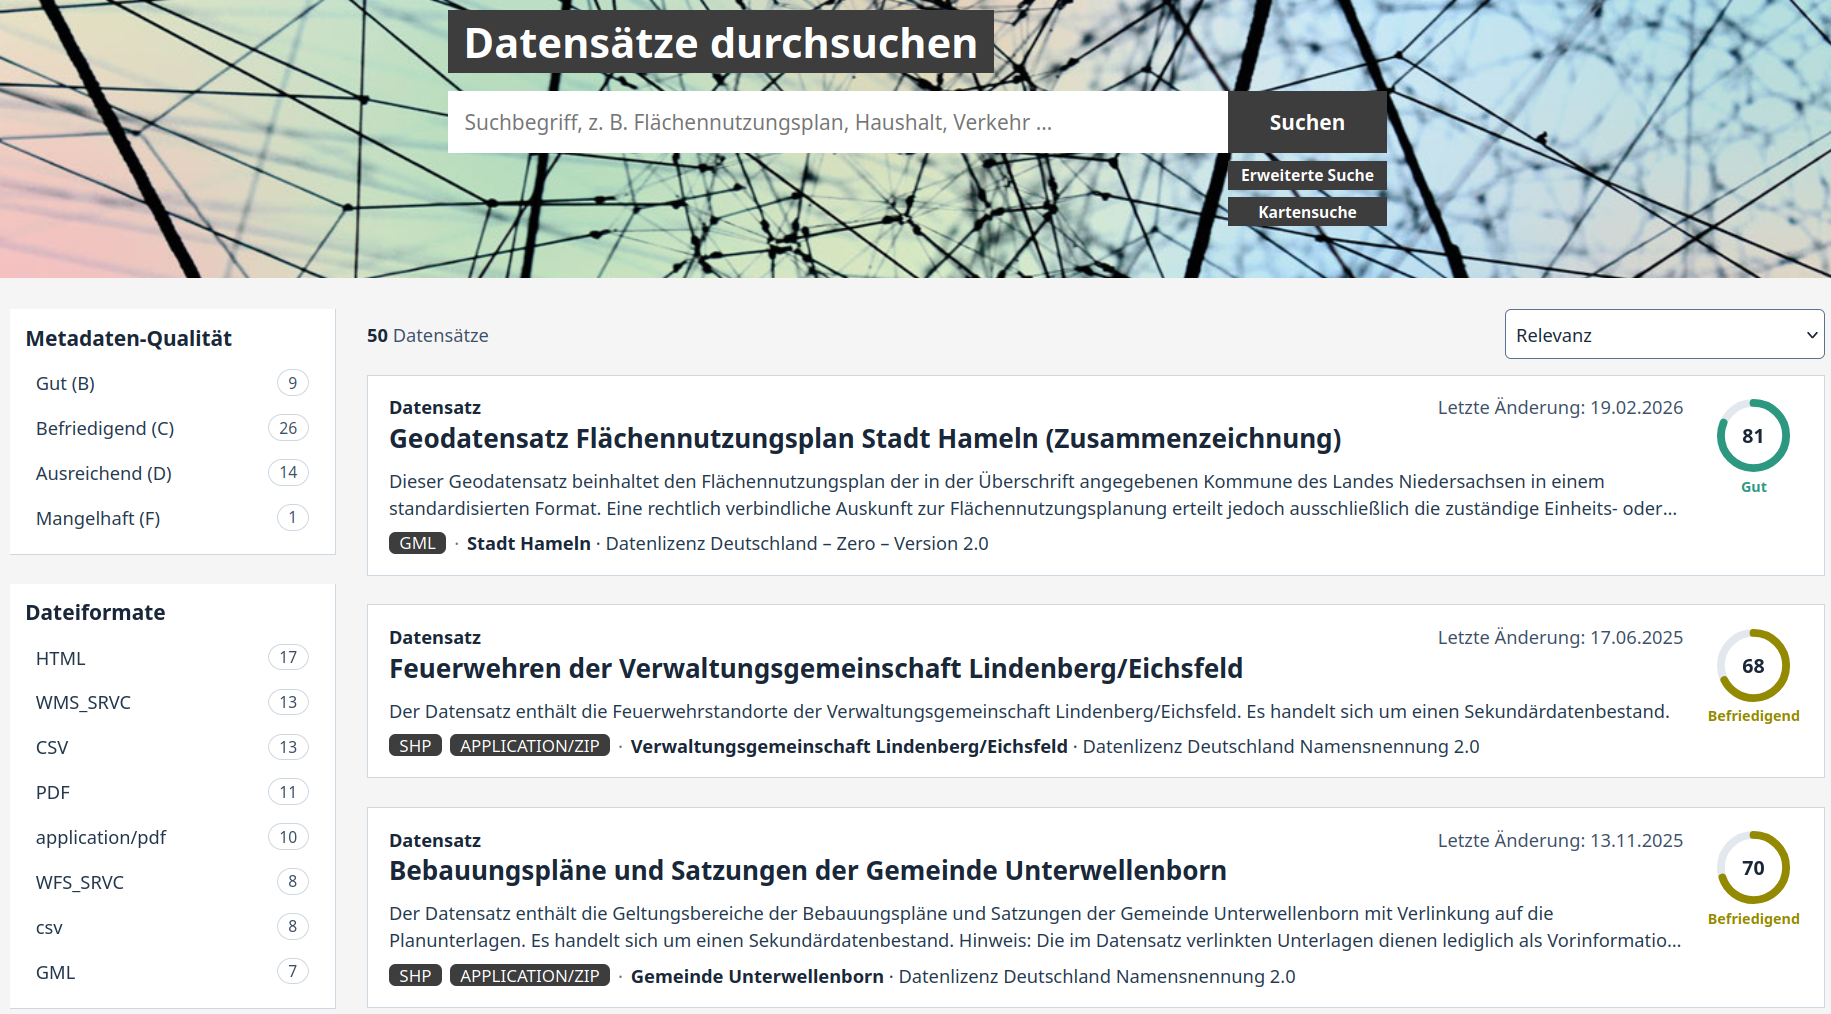
\includegraphics[width=\textwidth]{images/einbettung_scoring_gesamtansicht_2.png}

    \captionsetup{justification=centering}
    \caption{Suchseite mit Qualitätsfacette links und Qualitätsring je Treffer}
    \label{fig:frontend_trefferliste}
\end{figure}

Abbildung~\ref{fig:frontend_trefferliste} zeigt die Suchseite dieser Nachbildung: Der Qualitätsring steht je Treffer rechts neben den beschreibenden Angaben, und die Qualitätsstufe tritt links als zusätzliche Facette neben die bestehenden Filter des Portals.
% Scope: Nur anreißen — welche Bausteine, welche Sprache, welches Protokoll.
% Die ausführliche Architektur des Bewertungskerns steht in
% Section~\ref{sec:architektur}; hier geht es allein um die Anbindung der
% Oberfläche.
\subsection{Anbindung an den Bewertungskern}
\label{subsec:frontend_architektur}

Die Oberfläche greift nicht auf den Bewertungskern zu, sondern spricht mit ihm über eine dazwischenliegende Dienstschicht. Diese ist in Python umgesetzt und bindet den in Section~\ref{sec:architektur} beschriebenen Bewertungsdienst als Bibliothek ein. Sie enthält selbst keine Bewertungslogik, sondern übersetzt zwischen Konfiguration, Ergebnisreport und Anzeigeform. Nach außen stellt sie eine HTTP-Schnittstelle bereit, über die sämtlicher Austausch in JSON erfolgt. Die Oberfläche ist eine im Browser laufende Anwendung in TypeScript und hält keinen eigenen Zustand über die dargestellten Ergebnisse hinaus.

Die Schnittstelle gliedert sich in vier Gruppen von Endpunkten: für die Datenbestände, für abgeschlossene Bewertungsläufe, zum Anstoßen neuer Läufe sowie für die Bewertungskonfiguration und den Klartext je Indikator. Auch Bezeichnung, betroffenes Feld, Handlungsanweisung und Vorlage stammen damit aus dem Bewertungskern und werden nicht in der Oberfläche gepflegt. Ein Lauf dauert wegen der Netzabfragen und des Sprachmodellaufrufs je Datei zu lange, um eine HTTP-Anfrage so lange offen zu halten. Die Anfrage legt deshalb nur einen Auftrag an und liefert dessen Kennung zurück, die Verarbeitung läuft im Hintergrund, und die Oberfläche fragt den Fortschritt zyklisch ab.

% Scope: Wie aus indikatorspezifischer Evidenz eine einheitliche Darstellung
% wird. Das Befundmodell (Kernaussage, Ist-Angaben mit Fundstelle, Hinweis als
% Handlungsanweisung, Einzelbefunde) als gemeinsame Form über alle Indikatoren
% hinweg. Warum der Befund im Backend entsteht. Die Verortung im RDF-Quelltext
% behandelt die folgende Subsection als eine der beiden Formen des Detailblocks.
\subsection{Vom Prüfergebnis zum Befund}
\label{subsec:befund}

Die Evidenz, die ein Indikator im Feld \texttt{details} des Reports hinterlegt, ist notwendigerweise indikatorspezifisch: Ein Erreichbarkeitsindikator hält Antwortstatus je Distribution fest, ein Konformitätsindikator die verletzten Regeln der Schemaprüfung, ein sprachmodellgestützter Indikator die Einzelbefunde und deren Begründung. Für die Darstellung ist diese Vielfalt hinderlich. Eine Oberfläche, die 27~unterschiedlich aufgebaute Evidenzstrukturen jeweils eigens darstellt, ist weder wartbar noch für den Leser erlernbar.

Der Prototyp überträgt deshalb jedes negative Prüfergebnis in eine einheitliche Form, den \emph{Befund}. Er besteht aus einer Kernaussage, die das Problem benennt, aus Ist-Angaben, die den vorgefundenen Zustand belegen und jeweils eine Fundstelle tragen können, aus einem Hinweis, der den geforderderten Zustand beschreibt, sowie aus Einzelbefunden für den Fall mehrerer gleichartiger Verstöße. Diese Form ist über alle Indikatoren hinweg identisch. Der Leser lernt sie einmal und kann sie danach auf jeden Indikator anwenden, unabhängig davon, ob dessen Urteil aus einer Feldprüfung, einer Netzabfrage oder einer Sprachmodellbewertung stammt. Als Fundstelle dient je nach Indikator die betroffene Distribution, der verletzte Pfad der Schemaprüfung oder das Feld. Der Hinweis ist bewusst als Handlungsanweisung und nicht als Zustandsbeschreibung formuliert. Er benennt, was zu tun ist, statt zu wiederholen, wie das Ergebnis aussähe, wenn es richtig wäre. Die Auflistung der nicht bestandenen Prüfungen mit Fundstelle und, wo möglich, Quelltextbeleg orientiert sich damit an der Form, die die Konformitätsprüfdienste des W3C für Markup und Stylesheets etabliert haben \cite{w3c_nu_checker, w3c_css_validator}: Deren Meldungen bestehen ebenfalls aus einem Schweregrad, einer natürlichsprachlichen Kernaussage, der Position in der Quelle und einem Auszug des Quelltexts um diese Position. Der Befund überträgt dieses Muster von der Syntaxprüfung eines Dokuments auf die Qualitätsprüfung eines Metadatensatzes. Abbildung~\ref{fig:frontend_befund} zeigt einen aufgeklappten Befund am Beispiel des Indikators zum Dateiformat: links die vorgefundenen Werte mit der jeweils betroffenen Distribution als Fundstelle, rechts der Hinweis mit dem Verweis auf das maßgebliche Vokabular.

\begin{figure}[H]
    \centering
    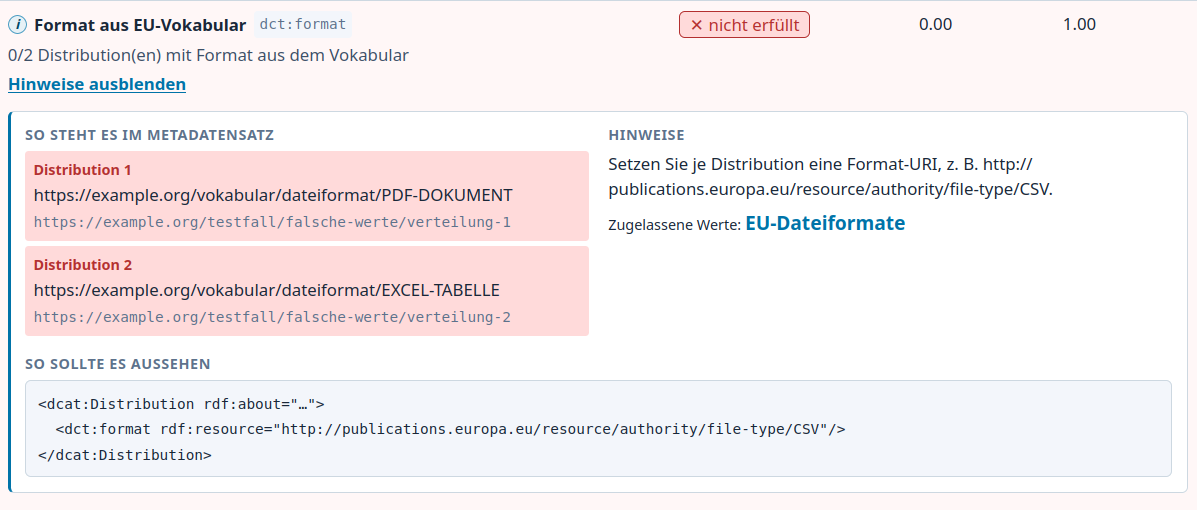
\includegraphics[width=\textwidth]{images/befund_nicht_erfuellter_einzelindikator.png}
    \captionsetup{justification=centering}
    \caption{Aufgeklappter Befund zu einem nicht erfüllten Indikator}
    \label{fig:frontend_befund}
\end{figure}

Der Befund entsteht im Bewertungskern und nicht in der Oberfläche. Die Übersetzung von Evidenz in eine Aussage über den Metadatensatz setzt Kenntnis des jeweiligen Indikators voraus und ist damit eine fachliche, keine gestalterische Entscheidung. Läge sie in der Oberfläche, entstünde eine zweite Interpretationsschicht neben dem Bewertungsmodell, Änderungen an einem Indikator müssten an zwei Stellen nachgezogen werden, und der maschinenlesbare Report wäre nicht mehr die einzige Quelle der Darstellung. Erzeugt wird ein Befund nur für nicht oder teilweise erfüllte Indikatoren sowie für Fehlerfälle. Bei einem erfüllten Indikator gibt es nichts zu erklären.

% Scope: Die zweite Aufbereitungsstufe — wie die geforderte Angabe konkret
% aussieht. Zwei Formen je Indikator: Vorlage oder Fundstelle im Quelltext.
% Entwurfsentscheidung: nicht die Menge der zulässigen Werte zeigen, sondern
% die Form der erwarteten Angabe.
\subsection{Von der Meldung zur Handlungsanweisung}
\label{subsec:handlungsanweisung}

Der Befund benennt das Problem und den Weg zu seiner Auflösung, beides jedoch in Prosa. Was er nicht leistet, ist die Übersetzung dieser Anweisung in die Schreibweise, die der Metadatensatz verlangt: Ein Datenbereitsteller ohne DCAT-Kenntnisse weiß nach dem Hinweis, dass eine Kategorie aus dem EU-Vokabular zu setzen ist, aber nicht, wie das im RDF/XML seines Datensatzes auszusehen hat. Die zweite Aufbereitungsstufe schließt diese Lücke.

Der Prototyp zeigt dafür eine \textbf{Vorlage}: ein kurzes RDF/XML-Fragment, dass das betroffene Feld in korrekter Schreibweise mit einem Beispielwert enthält. Damit entfällt die Hürde, erst nachschlagen zu müssen, wie die geforderte Angabe zu notieren ist -- welches Feld, welche Verschachtelung, welche Schreibweise steht unmittelbar vor dem Adressaten. Geht es um ein Feld mit kontrolliertem Vokabular, stehen im Hinweis daneben zusätzlich die Bezeichnung des Vokabulars und der Verweis auf dessen Übersichtsseite, sodass sich der inhaltlich passende Wert dort auswählen lässt. Abbildung~\ref{fig:frontend_handlungsanweisung}\,(\subref{fig:frontend_detailblock_vorlage}) zeigt eine solche Vorlage für die Geometrieangabe eines Datensatzes.

Entscheidend für den Nutzen der Vorlage ist, dass sie unabhängig vom vorgefundenen Zustand ist. Sie sieht identisch aus, ob das Feld falsch belegt ist oder ganz fehlt. Gerade der zweite Fall ist der, in dem sie gebraucht wird, denn dort gibt es im Metadatensatz nichts, worauf sich zeigen ließe.

Die Vorlagen zeigen die geforderte Schreibweise damit feldweise und jeweils nur für den einen Indikator, an dem der Datensatz gescheitert ist. Zusammengesetzt ergeben sie genau das Bild, das der Referenzdatensatz aus Abschnitt~\ref{sec:referenzdatensatz} als Ganzes vorführt: Was die Oberfläche einem Bereitsteller Feld für Feld und anlassbezogen zeigt, steht dort einmal vollständig und in sich stimmig. Beide Darstellungen bedienen dieselbe Frage: Wie sieht die richtige Angabe aus? Und wird durch zwei Auflösungsstufen, der Einzelfeldvorlage im Bearbeitungsfluss und dem vollständigen Beispieldatensatz als Ganzes beantwortet.



\begin{figure}[H]
    \centering
    \begin{subfigure}{\textwidth}
        \centering
        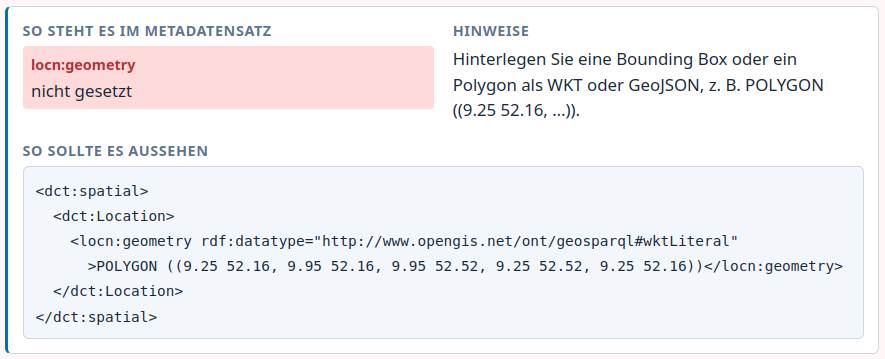
\includegraphics[width=\textwidth]{images/so_sollte_es_aussehen_ansicht.png}
        \captionsetup{justification=centering}
        \caption{Vorlage („So sollte es aussehen“) für ein Feld mit vorgegebener Schreibweise}
        \label{fig:frontend_detailblock_vorlage}
    \end{subfigure}
    \\[1em]
    \begin{subfigure}{\textwidth}
        \centering
        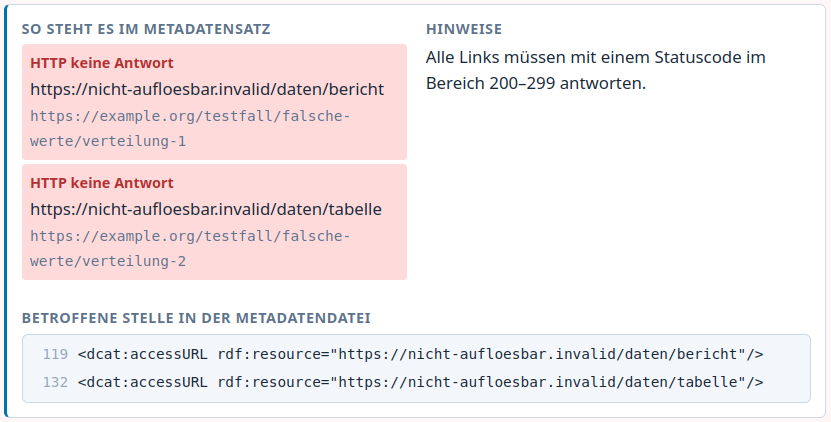
\includegraphics[width=\textwidth]{images/betroffene_stelle_in_den_metadaten_ansicht.png}
        \captionsetup{justification=centering}
        \caption{Fundstelle („Betroffene Stelle in der Metadatendatei“) für einen inhaltsabhängigen Indikator}
        \label{fig:frontend_detailblock_fundstelle}
    \end{subfigure}
    \captionsetup{justification=centering}
    \caption{Die beiden Formen des Detailblocks: Vorlage und Fundstelle im Quelltext}
    \label{fig:frontend_handlungsanweisung}
\end{figure}

Nicht jeder Indikator lässt eine solche Vorlage zu. Wenn die richtige Angabe vom Inhalt abhängt und nicht von der Schreibweise, wie Beispielsweise bei den Schlagwörtern oder sprachmodellgestützten Indikatoren, gäbe eine Vorlage nur eine Syntax vor, die ohnehin nie das Problem war. Das selbe gilt auch für Indikatoren, wo das Problem außerhalb des Metadatensatzes liegt, etwa bei einem Verweis, der ins Leere führt. Für diese Indikatoren tritt an die Stelle der Vorlage die \textbf{Fundstelle}: die einschlägigen Zeilen des RDF-Quelltexts mit Zeilennummer, sodass sich die Kette von der Punktzahl bis zur konkreten Stelle im Metadatensatz schließt.
Abbildung~\ref{fig:frontend_handlungsanweisung}\,(\subref{fig:frontend_detailblock_fundstelle}) zeigt dies für zwei nicht auflösbare Verweise. Für eine dritte Gruppe schließlich entfällt der Detailblock ganz, weil Befund und Hinweis bereits alles tragen. 

Welche der drei Formen ein Indikator führt, ist damit keine Eigenschaft des Einzelergebnisses, sondern des Indikators, und liegt entsprechend als feste Angabe neben Klarnamen, Feldbezeichnung und Handlungsanweisung im Bewertungskern. Der Detailblock trägt in jedem Fall genau eine dieser Formen.
% Scope: Die Sichten und ihre Zuordnung zu den Zielgruppen aus
% Tabelle~\ref{tab:zielgruppen}. Barrierefreiheit: Farbe nie alleiniger
% Bedeutungsträger, nachgerechnete Kontraste.
\subsection{Darstellung und Bedienung}

Den drei Zielgruppen aus Tabelle~\ref{tab:zielgruppen} entsprechen drei Auflösungsstufen der Darstellung. Sie folgen dem Ordnungsprinzip \emph{Überblick zuerst, dann Filtern, dann Details auf Anforderung}, das Shneiderman als Grundmuster informationsvisualisierender Oberflächen beschreibt \cite{shneiderman1996eyes}: Jede Stufe zeigt so viel, wie die Entscheidung auf dieser Ebene erfordert, und macht die nächste Detailtiefe erst auf Anforderung sichtbar. Die Trefferliste zeigt je Datensatz allein den Gesamtscore als Ring mit Note und bedient damit die Auswahlentscheidung der Datennutzenden, ohne die Liste mit Bewertungsdetails zu überfrachten.

Die Detailsicht eines Datensatzes richtet sich an die Datenbereitstellenden. Sie zeigt den Gesamtscore, das Profil über die vier Qualitätsdimensionen als Netzdiagramm und darunter je Dimension eine Übersicht ihrer Indikatoren mit Ergebnisstufe, Punktwert und Gewicht; jeder nicht erfüllte Indikator lässt sich zu dem in Section~\ref{subsec:befund} beschriebenen Befund aufklappen. Zwei Bedienelemente steuern den Umfang der Ansicht: Ein Schalter blendet die erfüllten Indikatoren aus und reduziert sie auf das, was zu bearbeiten ist. Ein weiterer Knopf klappt Dimensionen und Befunde gemeinsam auf oder zu und macht damit den vollständigen Bearbeitungsbedarf eines Datensatzes in einem Schritt sichtbar, statt ihn Dimension für Dimension und darin Befund für Befund erschließen zu lassen. Abbildung~\ref{fig:frontend_detailsicht} zeigt diesen Bewertungsabschnitt im eingeklappten Zustand: Note, Gesamtscore und Dimensionsprofil als Einstieg, darunter je Dimension eine Zeile, die neben Score und Gewicht ausweist, wie viele ihrer Indikatoren erfüllt sind und wie viele Handlungsbedarf auslösen.

\begin{figure}[H]
    \centering
    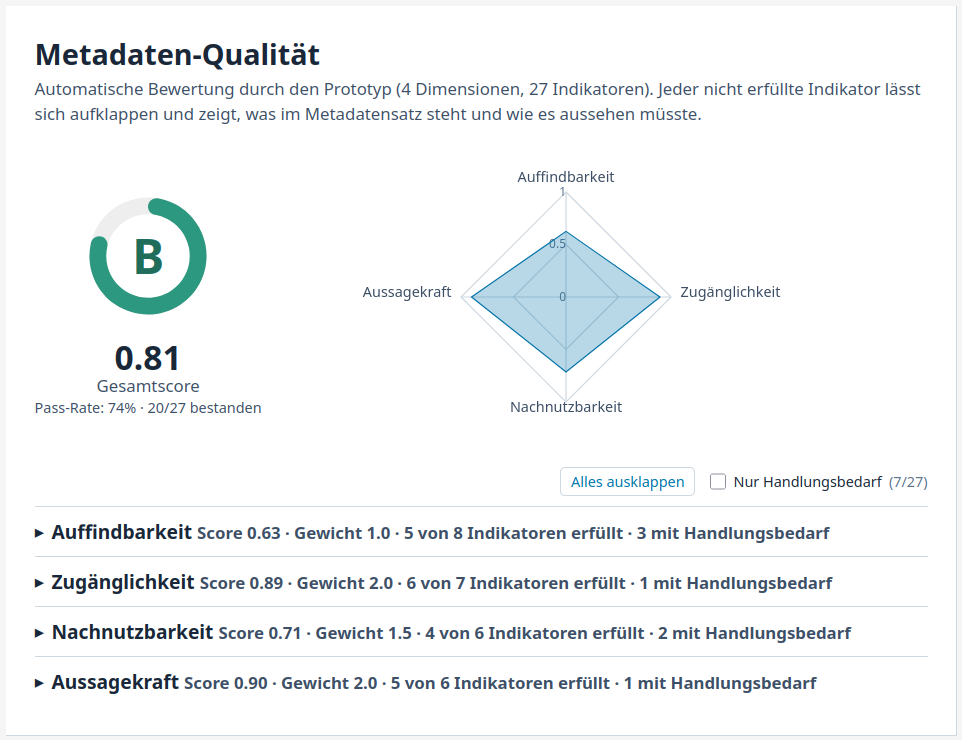
\includegraphics[width=\textwidth]{images/einzelansicht_uebersicht_metadatenqualitaet.png}
    \captionsetup{justification=centering}
    \caption{Detailsicht eines Datensatzes mit Dimensionsprofil und Indikatorübersicht}
    \label{fig:frontend_detailsicht}
\end{figure}

Die Aggregationsicht in Abbildung~\ref{fig:frontend_aggregatsicht} bedient die Portalbetreibenden. Sie weist die Zahl der bewerteten Datensätze, den mittleren Gesamtscore mit Spannweite und den Anteil erfüllter Prüfungen aus und ergänzt diese Kennzahlen um die Verteilung der Gesamtbewertung, die Mittelwerte je Dimension, die häufigsten Mängel als Anteil der Datensätze, die einen Indikator nicht oder nur teilweise erfüllen, sowie den Verlauf über die vorliegenden Bewertungsläufe. Die Zusammenstellung folgt dem für Übersichtsdarstellungen formulierten Grundsatz, die zur Beurteilung erforderlichen Größen gemeinsam und nach ihrem Informationswert geordnet zu zeigen, statt sie auf mehrere Ansichten zu verteilen \cite{few2006dashboard}. Die Verlaufsdarstellung ist bewusst zurückhaltend beschriftet, weil ihre Punkte Bewertungsläufe und keine Erhebungszeitpunkte sind: Sie zeigt zunächst die Streuung des Verfahrens und wird erst dann zu einer Qualitätsentwicklung, wenn der Bestand wiederholt geharvestet und bewertet wird.

\begin{figure}[H]
    \centering
    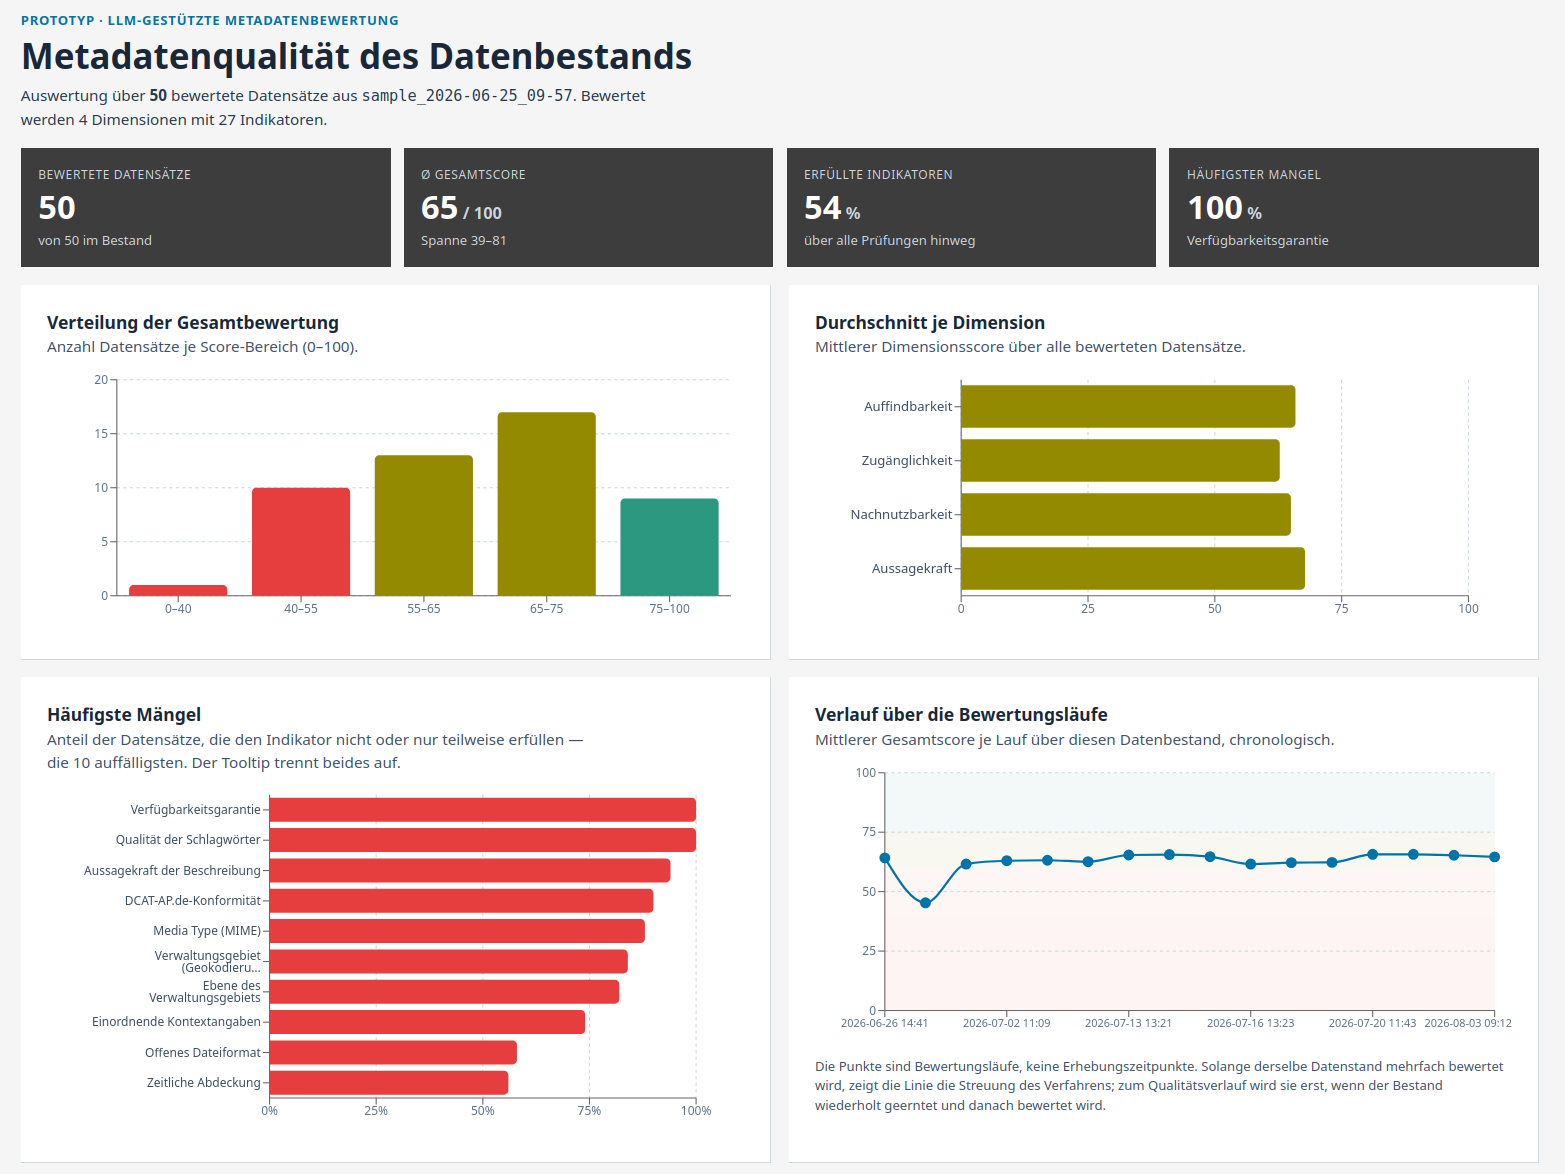
\includegraphics[width=\textwidth]{images/gesamtansicht_aggregation_portalweit.png}
    \captionsetup{justification=centering}
    \caption{Aggregatsicht über einen Datenbestand}
    \label{fig:frontend_aggregatsicht}
\end{figure}

Für die aus der Oberfläche angestoßenen Bewertungsläufe gilt eine Vorgabe, die für die Belastbarkeit der dargestellten Werte wesentlich ist: Die Oberfläche führt keine eigenen Voreinstellungen, sondern lädt zur Laufzeit dieselbe Konfigurationsdatei, die auch der Evaluation dieser Arbeit zugrunde liegt. Gewichte, Punktevergabe und Indikatormenge sind damit nicht nur ähnlich, sondern identisch. Als einzige Wahl bleibt, ob die sprachmodellgestützte Dimension der Aussagekraft einbezogen wird. Eine Unterscheidung, die auf Zeit- und Kostenaufwand des Laufs durchschlägt.

Für die Gestaltung gelten durchgängig zwei Regeln der Barrierefreiheit, die den Web Content Accessibility Guidelines entnommen sind \cite{w3c_wcag22}. Farbe ist nie alleiniger Bedeutungsträger (Erfolgskriterium~1.4.1): Jede Ergebnisstufe trägt neben ihrer Farbe ein Symbol und eine ausgeschriebene Bezeichnung, jede Diagrammreihe ist beschriftet. Sämtliche Farbwerte stammen aus dem Gestaltungssystem des Portals; ihre Kontraste wurden für die verwendeten Kombinationen gegen die Schwellen der Erfolgskriterien~1.4.3 und~1.4.11 nachgerechnet, statt sie nach Augenmaß zu wählen. Ergänzend wurden die Diagrammfarben mit einem physiologisch begründeten Simulationsmodell für Farbfehlsichtigkeit \cite{machado2009cvd} auf ihre Unterscheidbarkeit geprüft.



\chapter{Evaluation}

\section{Evaluationsdesign und Hypothesen}
\label{sec:eval_design}

Die Evaluation stützt sich auf zwei komplementäre Argumentationsstränge, die auf identischem
RDF-Input erhoben werden. Der erste vergleicht den Prototyp mit einem unabhängig
erhobenen menschlichen Referenzurteil und beantwortet die Frage, ob er \emph{korrekt} bewertet.
Der zweite vergleicht ihn mit der Metadata Quality Assessment (MQA) von data.europa.eu als
etablierter Baseline und beantwortet die Frage, was er \emph{ergänzend} sieht. Beide
Stränge sind aufeinander aufbauend: Der Baseline-Vergleich allein kann lediglich zeigen,
dass sich die Bewertungen unterscheiden, nicht aber, welche der beiden näher an der
tatsächlichen Qualität liegt. Erst der Ground-Truth-Vergleich erlaubt diese Aussage.

Daraus ergeben sich drei Hypothesen: 

\begin{enumerate}

    \item \textbf{H1 (Konvergenz):} Die Scores beider Verfahren konvergieren stark auf denjenigen Indikatoren, die äquivalent geprüft werden. Methodisch entspricht dies dem Nachweis konvergenter Validität~\cite{campbell1959convergent}.
    \item \textbf{H2 (Mehrwert):} Die Scores divergieren systematisch auf denjenigen Indikatoren, bei denen der Prototyp tiefer prüft als die MQA oder bei denen die MQA über kein Pendant verfügt. Eine solche Divergenz ist dabei kein Fehler, sondern der erwartete Effekt des verifizierenden statt lediglich prüfenden Ansatzes.
    \item \textbf{H3 (Korrektheit):} Auf denjenigen Indikatoren, auf denen beide Verfahren divergieren, stimmt der Prototyp stärker mit dem Referenzurteil überein als die MQA. H3 verbindet beide Argumentationsstränge und trägt die eigentliche Überlegenheitsaussage: Ohne sie belegt H2 nur, dass anders gemessen wird, nicht dass besser gemessen wird.

\end{enumerate}

\section{Datengrundlage und Stichprobe}
\label{sec:eval_stichprobe}

Grundlage der Evaluation ist ein vollständiger Auszug des GovData-CKAN-Katalogs vom
15.~Mai~2026 mit 151.579 Datensätzen. Aus diesem wurden zunächst alle Datensätze
entfernt, die mindestens eine NetCDF-Distribution enthalten (1.793 Datensätze,
verbleibend 149.786). NetCDF-Ressourcen sind typischerweise sehr große Klima- und
Umweltdatenreihen, deren Abruf im Rahmen der technischen Erreichbarkeitsprüfung
Laufzeit und Datenvolumen dominiert hätte, ohne inhaltlich zusätzliche Erkenntnisse zu
liefern. Der verbleibende Katalog wurde anhand von Formatangaben, Medientypen und
Service-Kennungen in 25.416 Geo-Datensätze und 124.370 Nicht-Geo-Datensätze unterteilt.

Aus dieser Grundgesamtheit wurde am 25.~Juni~2026 eine \textbf{stratifizierte
Zufallsstichprobe} von $n = 50$ Datensätzen gezogen (Seed~67, reproduzierbar über
Notebook~12\footnote{\url{https://github.com/LarsBuergerr/master_thesis_prototype/blob/v3_prototype_freeze/playground/notebooks/12_fetch_stratified_sample.ipynb}}). Die Gruppierung erfolgt zweistufig: primär nach der Unterscheidung
Geo/Nicht-Geo, sekundär innerhalb beider Gruppen nach den vier jeweils
aufkommensstärksten Datenbereitstellern zuzüglich einer Restkategorie für alle übrigen
Bereitsteller. Aus jedem der so entstehenden zehn Straten werden fünf Datensätze gezogen.
Die Schichtung stellt sicher, dass die Stichprobe die für die Metadatenqualität
relevanten Unterschiede der Grundgesamtheit abbildet, statt von den wenigen
aufkommensstärksten Portalen dominiert zu werden, die bei einer einfachen Zufallsziehung
den Großteil der Stichprobe stellen würden. Die gezogenen Datensätze wurden anschließend
als RDF/XML von GovData abgerufen und bilden damit denselben Input, auf dem der Prototyp 
und die MQA-Reimplementierung arbeiten.

Ergänzend zur Kernstichprobe steht ein Satz von zwanzig \textbf{kuratierten Extremfällen}
zur Verfügung, je zehn mit erwartbar hoher und erwartbar niedriger Metadatenqualität.
Erstere zeichnen sich durch eine aussagekräftige Beschreibung, erreichbare Ressourcen,
maschinenlesbare Formate sowie vorhandene Lizenz- und Kontaktangaben aus, letztere durch
generische Titel, nichtssagende Beschreibungen, defekte Verweise, unklare Lizenzen und
fehlerhafte Formatangaben. Beide Schichten verfolgen unterschiedliche Zwecke und werden 
getrennt ausgewertet: Die Extremfälle belegen den Wirkmechanismus per
Konstruktion, da bei ihnen bekannt ist, welches Ergebnis zu erwarten ist. Die
Kernstichprobe kontrolliert die Selektionsverzerrung, die einer kuratierten Auswahl
notwendigerweise anhaftet, und zeigt das Verhalten unter realistischen Bedingungen.
Da die Extremfälle konstruiert und nicht randomisiert selektiert sind, erlauben sie keine
Verallgemeinerung auf die Grundgesamtheit. Alle quantitativen Aussagen dieser Arbeit
stützen sich daher durchgehend auf die Kernstichprobe.

\section{Ground-Truth-Erhebung}

Als Maßstab dient eine manuelle Referenzbewertung aller 50 Datensätze der
Kernstichprobe und der Extremfälle entlang derselben vier Qualitätsdimensionen, die in
Kapitel~4 hergeleitet wurden (Tabelle~\ref{tab:finale-qualitaetsdimensionen}) und die der
Prototyp gemäß Kapitel~5 operationalisiert. Diese Referenzbewertung wurde nicht durch
eine unbeteiligte dritte Person, sondern im Rahmen dieser Arbeit selbst vorgenommen. Wo
im Folgenden von einem \emph{unabhängigen} Maßstab die Rede ist, bezieht sich das
ausschließlich auf die methodische Trennung von der Prüflogik des Prototyps, nicht auf
eine personelle Unabhängigkeit. Bewertet wird jede Dimension auf einer
sechsstufigen Skala von 0 bis 5 entlang je einer ausformulierten Ankerfrage.
Tabelle~\ref{tab:gt_anker} führt die vier Fragen auf. Die Stufenzahl folgt dem Befund von
Preston und Colman~\cite{preston2000optimal}, wonach Reliabilität, Validität und
Diskriminierungsfähigkeit von Ratingskalen auf etwa fünf bis sieben Stufen zunehmen
und vierstufige Skalen suboptimal sind. Da die Stufenzahl gerade ist, besitzt die Skala
keinen Mittelpunkt, auf den Bewertende bei Unsicherheit ausweichen könnten
(Central-Tendency-Bias). Hinzu kommt, dass jede Dimension durch eine feste, inhaltlich
definierte Ankerfrage konkretisiert ist (Tabelle~\ref{tab:gt_anker}), sodass sich eine
Einschätzung an einem konkreten Kriterium statt an einer unspezifischen Präferenz
festmachen lässt.



\begin{table}[H]
\centering
\scriptsize
\renewcommand{\arraystretch}{1.3}
\rowcolors{1}{white}{white}
\begin{tabularx}{\textwidth}{p{0.20\textwidth} X}
\hline
\textbf{Dimension} & \textbf{Ankerfrage} \\
\hline
Auffindbarkeit &
Ist der Datensatz über Titel, Beschreibung, Schlagwörter, Kategorien sowie räumliche
und zeitliche Angaben gut auffindbar und einordenbar? \\
\hline
Zugänglichkeit &
Sind die beschriebenen Distributionen erreichbar, abrufbar, maschinenlesbar und technisch
plausibel beschrieben? \\
\hline
Nachnutzbarkeit &
Sind Lizenz, Rechte, Kontakt, Herausgeber und verwendete Vokabulare für eine
Weiterverwendung ausreichend klar? \\
\hline
Aussagekraft &
Sind Titel, Beschreibung, Schlagwörter und Kontextangaben verständlich, plausibel und
informationshaltig? \\
\hline
\end{tabularx}
\caption{Ankerfragen der manuellen Ground-Truth-Bewertung je Qualitätsdimension}
\label{tab:gt_anker}
\end{table}

Methodisch entscheidend ist, dass die Anker die \emph{nutzerseitige Qualitätserfahrung}
beschreiben und nicht die Indikatorlogik des Prototyps. Ein Anker der Dimension
Auffindbarkeit formuliert beispielsweise, ob ein Nutzer den Datensatz über seine
Metadaten finden und thematisch einordnen kann, nicht ob ein bestimmtes DCAT-Feld belegt
ist. Damit misst die Ground Truth dasselbe Konstrukt aus methodisch unabhängiger
Perspektive, statt die Prüflogik des Prototyps manuell
nachzuvollziehen~\cite{campbell1959convergent}.

Aus den vier Dimensionswerten wird ein Gesamturteil in den Stufen \emph{gut},
\emph{mittel} und \emph{schlecht} abgeleitet. Tabelle~\ref{tab:gt_gesamturteil} führt die
Schwellen auf.

\begin{table}[H]
\centering
\scriptsize
\renewcommand{\arraystretch}{1.2}
\rowcolors{1}{white}{white}
\begin{tabular}{p{0.13\textwidth} p{0.28\textwidth} p{0.38\textwidth}}
\hline
\textbf{Gesamturteil} & \textbf{Durchschnitt der vier Dimensionen} & \textbf{Zusätzliche Bedingung} \\
\hline
gut & mindestens 4,0 & keine Dimension unter 3 \\
\hline
schlecht & höchstens 2,0 & -- \\
 & oder unter 3,5 & mindestens zwei Dimensionen unter 2 \\
\hline
mittel & \multicolumn{2}{p{0.68\textwidth}}{alle übrigen Fälle} \\
\hline
\end{tabular}
\caption{Ableitung des Gesamturteils der Ground Truth aus den vier Dimensionswerten}
\label{tab:gt_gesamturteil}
\end{table}

Die Schwellen in Tabelle~\ref{tab:gt_gesamturteil} legen inhaltlich fest, was ein
\emph{gutes}, \emph{mittleres} oder \emph{schlechtes} Ergebnis trennt, unabhängig
davon, wie sich die konkrete Stichprobe zufällig verteilt und orientieren sich an der kriteriumsorientierten Messung nach Glaser~\cite{glaser1963}. Sie wurden
also nicht nachträglich so gewählt, dass eine bestimmte Verteilung von
gut/mittel/schlecht herauskommt.

Die Ableitungsregel kombiniert zwei Bedingungen. Erstens zählt der Durchschnitt der vier
Dimensionswerte (mittlere Spalte der Tabelle): Ein hoher Wert in einer Dimension kann
einen niedrigeren Wert in einer anderen teilweise ausgleichen. Zweitens gilt zusätzlich
eine feste Sperrbedingung (rechte Spalte): Fällt eine einzelne Dimension zu stark ab,
verhindert das die Note \emph{gut} unabhängig vom Durchschnitt. Diese Kombination stellt
sicher, dass ein gravierender Mangel in nur einer Dimension, etwa eine unklare Lizenz
bei ansonsten guten Metadaten, nicht einfach im Durchschnitt der übrigen drei
Dimensionen verschwindet~\cite{einhorn1971}.

Die Bewertung erfolgte blind gegenüber den Ergebnissen des Prototyps: Die
Bewertungsvorlage enthält ausschließlich den Inhalt der zu bewertenden Metadatendatei
 nicht jedoch dessen Scores. Damit wird ein
Anchoring-Bias ausgeschlossen, der die gemessene Übereinstimmung künstlich erhöhen würde.

Aus der eingangs genannten fehlenden unabhängigen Person der Referenzbewertung folgen zwei Einschränkungen. Eine Inter-Rater-Reliabilität kann nicht
bestimmt werden, und ein Bestätigungsfehler durch Vorwissen über das Bewertungsmodell
lässt sich nicht vollständig ausschließen.

\section{Vergleichsbaseline: MQA-Reimplementierung und A/B/C-Klassifikation}
\label{sec:eval_mqa_abc}

Als Vergleichsmaßstab dient die Metadata Quality Assessment Implementierung von data.europa.eu. Sie
eignet sich als Baseline, weil sie im europäischen Open-Data-Kontext etabliert ist,
ihre Methodik offengelegt ist und sie denselben DCAT-AP-Input bewertet wie der Prototyp.
Um beide Verfahren auf exakt derselben Datengrundlage vergleichen zu können, wurde die
MQA-Bewertungslogik nach der offiziellen Methodik~\cite{dataeuropa2024mqa}
reimplementiert und gegen die veröffentlichten Berichte von data.europa.eu validiert.
Wo die Methodik die Berechnung nicht abschließend festlegt, insbesondere bei der
Behandlung mehrerer Distributionen, wurde die Logik ergänzend aus dem öffentlichen
Quellcode des MQA-Scoring-Dienstes nachvollzogen~\cite{piveauMetricsScore}.
Die Reimplementierung ist dabei lediglich Evaluationsinstrument und nicht Bestandteil des
Artefakts. Da beide Verfahren unterschiedliche Punkteskalen verwenden, werden die
Ergebnisse vor dem Vergleich auf einen gemeinsamen Wertebereich normalisiert.

Der inhaltliche Kern des Vergleichs ist die Unterscheidung zweier Prüfparadigmen. Die MQA
bewertet überwiegend, \emph{ob} ein Feld vorhanden, in einem kontrollierten Vokabular
gelistet oder eine URL auflösbar ist. Sie nimmt Qualität bei Vorhandensein weitgehend an.
Der Prototyp prüft darüber hinaus, ob die vorhandenen Angaben gültig, untereinander
kongruent und inhaltlich tragfähig sind. Um diesen Unterschied systematisch auswertbar zu
machen, wird jeder Indikator des Prototyps einer von drei Klassen zugeordnet.

\begin{itemize}
    \item \textbf{Klasse~A} umfasst Indikatoren, die im Kern dasselbe prüfen wie eine
    MQA-Metrik. Hier ist hohe Übereinstimmung zu erwarten (H1).

    \item \textbf{Klasse~B} umfasst Indikatoren, bei denen die MQA bereits das Vorhandensein honoriert, während der Prototyp Gültigkeit oder Kongruenz verifiziert. Eine Kombination aus MQA-PASS und Prototyp-FAIL ist hier der Nachweis einer Überschätzung durch die MQA (H2).

    \item \textbf{Klasse~C} umfasst Indikatoren ohne MQA-Pendant, darunter die gesamte Dimension
    der Aussagekraft, bei denen die MQA strukturell blind bleibt, der Prototyp aber
    variiert (H2).
\end{itemize}

Diese Partitionierung entspricht klassischen Validitätsbegriffen der
Messtheorie~\cite{cronbach1955construct}: Klasse~A adressiert konvergente Validität,
Klasse~B und~C die inkrementelle Validität des Prototyps gegenüber der Baseline. Die
Zuordnung ist vollständig dokumentiert und enthält je Indikator die zugeordneten
MQA-Metriken, die Aggregationsregel und die Begründung. Die vollständige
Zuordnungstabelle findet sich in Anhang~\ref{app:mqa_abc_mapping}.


% @TODO das mal noch etwas weniger belastend formulieren am ende wird man deswegen zerrissen.
Damit der Vergleich nicht einseitig zugunsten des Prototyps ausfällt, sind umgekehrt auch
die MQA-Metriken zu nennen, für die der Prototyp keine Entsprechung vorsieht:
\texttt{rights\_availability} (\texttt{dct:rights}) und \texttt{byte\_size\_availability}
(\texttt{dcat:byteSize}). Beide Felder sind nach DCAT-AP.de weder verpflichtend noch
empfohlen. Bereits die Experteninterviews ordneten wenig aussagekräftige Zusatzfelder
dieser Art unter dem Prinzip \enquote{Qualität statt Quantität} als für die Bewertung
verzichtbar ein (Anhang~\ref{app:kodierleitfaden}, Kategorie K1.2), weshalb der Prototyp
hierfür keinen eigenen Indikator vorsieht.

\section{Auswertungsverfahren und Kennzahlen}
\label{sec:eval_auswertungsverfahren}

Für den Ground-Truth-Vergleich ist die \textbf{Spearman-Rangkorrelation $\rho$} die
Primärmetrik, berichtet als Gesamtwert und je Dimension. Die naheliegende Alternative
wäre ein Übereinstimmungsmaß auf dem dreistufigen Gesamturteil, üblicherweise
\textbf{Cohens $\kappa$}, das aus der beobachteten Übereinstimmung zwischen
Prototyp-Urteil und Ground Truth den Anteil herausrechnet, der bereits durch Zufall zu
erwarten wäre. Dass stattdessen $\rho$ die Entscheidungsgrundlage bildet und $\kappa$
nur ergänzend berichtet wird, hat drei
Gründe. Erstens ist die Forschungsfrage ordinal: Zu prüfen ist, ob der Prototyp die gleiche
Rangordnung erzeugt wie ein menschlicher Bewerter. Der kontinuierliche Score ist das
eigentliche Ergebnis des Verfahrens, das dreistufige Urteil lediglich eine daraus
abgeleitete Diskretisierung. Zweitens ist $\kappa$ auf dieser Stichprobe strukturell nach
oben begrenzt: Die Urteilsverteilung der Ground Truth ist mit rund
88\,\% der Datensätze in der Kategorie \emph{mittel} stark konzentriert, wodurch die
zufällig zu erwartende Übereinstimmung bereits bei etwa 0,79 liegt. Selbst ein nahezu
perfektes Verfahren könnte unter diesen Randbedingungen kein hohes $\kappa$ erreichen. Das ist
ein bekanntes Phänomen, das als Kappa-Paradox beschrieben
ist~\cite{feinstein1990kappa}. Dass eine reale, stratifiziert gezogene
GovData-Stichprobe überwiegend mittelmäßige Metadaten enthält, ist ein Befund über die
Datenlage, kein Mangel des Prototyps. Drittens ist der $\kappa$-Punktschätzer bei so
wenigen Fällen außerhalb der mittleren Kategorie instabil. Wie unsicher dieser eine
berichtete Wert ist, zeigt ein Bootstrap-Konfidenzintervall: Aus der vorhandenen
Stichprobe werden wiederholt neue, gleich große Stichproben mit Zurücklegen gezogen und
$\kappa$ jeweils neu berechnet. Die Bandbreite dieser wiederholten Berechnungen zeigt,
wie stark der Wert allein durch die zufällige Zusammensetzung der Stichprobe schwanken
würde. Für die Kernstichprobe reicht dieses Intervall von $0{,}18$ bis $0{,}92$ und
überspannt damit den gesamten Bereich von schwacher bis nahezu perfekter
Übereinstimmung. Das ist das stärkste Einzelargument gegen die Verwendung von $\kappa$
als Entscheidungsgrundlage.

Ergänzt wird die Rangkorrelation durch Kendalls $\tau$, eine weitere, robustere
Rangkorrelation, sowie durch eine Ceiling-Analyse.
Diese berechnet, welches $\rho$ bei der vorliegenden Ground-Truth-Verteilung überhaupt
erreichbar wäre, und zeigt damit, wie nah der Prototyp an dieses Maximum herankommt. Da
Rangkorrelationen ausschließlich die Reihenfolge und nicht das Niveau bewerten, treten
mittlerer absoluter Fehler (MAE) und Bias als Kalibrierungsmaße hinzu.

Auf der Urteilsebene, dem aus den vier Dimensionswerten abgeleiteten dreistufigen
Gesamturteil \emph{gut}/\emph{mittel}/\emph{schlecht}, werden ergänzend fünf
\textbf{Sekundärmetriken} berichtet:

\begin{itemize}
    \item \textbf{Accuracy} ist der Anteil korrekt vorhergesagter Urteile: leicht
    verständlich, aber bei der stark ungleichen Urteilsverteilung der Ground Truth
    (88\,\% \emph{mittel}) irreführend: Ein Verfahren, das unabhängig vom Datensatz
    immer \emph{mittel} vorhersagt, erzielt bereits eine hohe Accuracy.
    \item \textbf{Gewichtetes Cohens $\kappa$} korrigiert die Übereinstimmung um den
    Anteil, der bei dieser Verteilung bereits durch Zufall zu erwarten wäre, ist aber,
    wie oben gezeigt, durch eben diese Verteilung strukturell gedeckelt und mit einem
    breiten Bootstrap-Konfidenzintervall behaftet.
    \item \textbf{PABAK} (Prevalence-Adjusted Bias-Adjusted Kappa) korrigiert $\kappa$
    zusätzlich um die Verzerrung durch die ungleiche Urteilsverteilung
    selbst~\cite{byrt1993bias} und macht dadurch sichtbar, dass die niedrige
    $\kappa$-Punktschätzung hier ein Verteilungs- und kein Qualitätsbefund ist.
    \item \textbf{AUC} (Fläche unter der ROC-Kurve) misst, wie gut das Verfahren
    \emph{gut} von den übrigen Urteilen trennt, ohne dass dafür eine konkrete Schwelle
    festgelegt werden muss. Ein Wert nahe 1,0 bedeutet nahezu perfekte Trennung, 0,5
    entspricht zufälligem Raten.
    \item Die \textbf{Konfusionsmatrix} zeigt für jede Kombination aus
    Ground-Truth-Urteil und Prototyp-Urteil, wie viele Datensätze darauf entfallen, und
    macht damit sichtbar, welche Urteile konkret verwechselt werden statt nur, wie oft.
\end{itemize}

Alle genannten Kennzahlen haben dieselbe Ursache für ihre Schwächen: Fast alle
Datensätze fallen in die Urteilskategorie \emph{mittel}. Naheliegend wäre daher der Einwand,
eine feiner gestufte Urteilsskala könne das beheben.
Kontrollrechnungen mit anderen Klasseneinteilungen zeigen jedoch, dass es nicht auf die
Stufenzahl ankommt, sondern darauf, wo die Schwellen relativ zur Stichprobenverteilung
liegen. Hinzu kommt: Je feiner die Skala, desto stärker nähert sich quadratisch
gewichtetes $\kappa$ einer Korrelation an. Es würde am Ende dasselbe messen wie $\rho$,
nur zusätzlich abhängig von der gewählten Stufenzahl und der Lage der Schwellen.

Für den MQA-Vergleich werden je Indikatorklasse eigene Kennzahlen berichtet: die
Übereinstimmungsrate für Klasse~A, die Überschätzungsrate für Klasse~B, die
Score-Varianz des Prototyps bei flacher MQA-Bewertung für Klasse~C sowie eine
Bland-Altman-Darstellung der Score-Differenzen über den gesamten Wertebereich (die
Differenz beider Scores je Datensatz, aufgetragen über deren Mittelwert).

\subsection{Deckenprüfung des Messinstruments am Referenzdatensatz}
\label{subsec:deckenpruefung}

Die bisher beschriebenen Kennzahlen beziehen sich auf die Übereinstimmung zwischen
Prototyp und menschlicher Bewertung. Sie beantworten eine Frage nicht, die vor allen
Ergebniszahlen steht: Ist das obere Ende der Skala überhaupt erreichbar? Fallen die
Werte einer Stichprobe überwiegend mittelmäßig aus, sind zwei Erklärungen möglich --
die bewerteten Metadaten sind mittelmäßig, oder das Verfahren misst systematisch zu
streng. Solange nicht gezeigt ist, dass ein Datensatz den Höchstwert erreichen
\emph{kann}, bleibt die zweite Erklärung offen. Die in Abschnitt~\ref{sec:messmodell}
eingeführten Mali verschärfen diesen Einwand zusätzlich, da sie einzelne
Indikatorbeiträge unter null drücken können.

Geprüft wird dies am Referenzdatensatz aus Abschnitt~\ref{sec:referenzdatensatz}, also
am konstruierten Idealfall: einem realen Portaldatensatz, der so lange ergänzt wurde,
bis er den Sollzustand des Bewertungsmodells vollständig verkörpert. Bewertet wird er
mit derselben Konfiguration und demselben Sprachmodell wie beide Stichproben.
Tabelle~\ref{tab:deckenpruefung} berichtet das Ergebnis.

\begin{table}[H]
    \centering
    \scriptsize
    \renewcommand{\arraystretch}{1.2}
    \rowcolors{1}{white}{white}
    \begin{tabular}{lrrr}
    \hline
    \textbf{Dimension} & \textbf{Score} & \textbf{Bestandene Indikatoren} & \textbf{Gewicht} \\
    \hline
    Auffindbarkeit & 1,000 & 8 von 8 & 1,0 \\
    Zugänglichkeit & 1,000 & 7 von 7 & 2,0 \\
    Wiederverwendbarkeit & 1,000 & 6 von 6 & 1,5 \\
    Aussagekraft & 0,972 & 6 von 6 & 2,0 \\
    \hline
    \textbf{Gesamtscore} & \textbf{0,991} & \textbf{27 von 27} & \\
    \hline
    \end{tabular}
    \captionsetup{justification=centering}
    \caption[Deckenprüfung am Referenzdatensatz]{Bewertung des Referenzdatensatzes je
    Dimension (Konfiguration \texttt{state\_evaluation\_final},
    GPT-5.5).}
    \label{tab:deckenpruefung}
\end{table}

Die drei deterministischen Dimensionen erreichen exakt den Höchstwert: Alle
21~regelbasierten und technischen Indikatoren werden bestanden, einschließlich der
Erreichbarkeitsprüfungen beider Distributionen und der SHACL-Konformitätsprüfung. Die
Skala ist in diesem Teil des Instruments also nach oben ausgeschöpft, und keiner der
Mali greift bei einem korrekt beschriebenen Datensatz. Damit ist der Einwand einer
systematisch zu strengen Messung für die regelbasierten Dimensionen ausgeräumt: Wo die
Stichproben niedrigere Werte zeigen, ist das ein Befund über die bewerteten Metadaten
und nicht über das Verfahren.

Die Aussagekraft bleibt mit $0{,}972$ knapp unter dem Höchstwert, obwohl alle sechs
Teilkriterien als erfüllt gewertet werden. Die Abzüge sind gering und liegen beim
Titel ($0{,}95$), den Schlagwörtern ($0{,}90$) und der Beschreibung ($0{,}98$); die
Begründungen des Modells nennen dort ausschließlich Abwägungen zwischen
konkurrierenden Rubrikforderungen, etwa zwischen atomaren und inhaltlich
spezifischen Schlagwörtern. Das Sprachmodell vergibt den vollen Punktwert
also auch dann nicht durchgängig, wenn die Rubrik keinen benennbaren Mangel mehr
findet. Für die Interpretation der Ergebniskapitel folgt daraus zweierlei: Die
Aussagekraftswerte sind nach oben faktisch bei etwa $0{,}97$ gedeckelt, weshalb
Abstände in diesem Bereich nicht überinterpretiert werden dürfen; und der Effekt
verstärkt die in Abschnitt~\ref{sec:eval_modellauswahl} berichtete Beobachtung, dass die semantische Bewertung
zu einer Kompression am oberen Skalenrand neigt.

Zwei Einschränkungen sind festzuhalten. Erstens ist diese Prüfung eine
Instrumentenprüfung und kein Qualitätsbefund: Der Referenzdatensatz ist konstruiert und
nicht zufällig gezogen, sein Ergebnis sagt nichts über die Verteilung realer
Portaldaten aus. Zweitens ist die Aussagekraftsbewertung nicht bitgenau reproduzierbar;
Wiederholungsläufe auf identischer Eingabe ergaben Gesamtscores zwischen $0{,}991$ und
$0{,}993$, was der in Abschnitt~\ref{sec:eval_modellauswahl} ermittelten Streuung des Verfahrens entspricht und
die Aussage der Deckenprüfung nicht berührt.

% Scope: Erste Ergebnis-Section und Weichenstellung fuer alles Folgende. Die Modellwahl
% wird hier mit dem in 5.1-5.5 aufgebauten Instrument entschieden; ab 5.7 wird
% ausschliesslich das gewaehlte Modell berichtet.
%
% Rahmung zuerst (traegt die ganze Section): Von den vier Dimensionen ist nur die
% Aussagekraft LLM-gestuetzt. Auffindbarkeit, Zugaenglichkeit und Wiederverwendbarkeit
% werden deterministisch aus dem RDF berechnet und liefern ueber alle Modelle exakt
% identische rho-Werte (0.5244 / 0.7119 / 0.7390). Die Modellwahl beruehrt also genau
% eine von vier Dimensionen -- Gesamtmetriken mischen den identischen deterministischen
% Teil bei und verwaessern den Vergleich. Der Vergleich wird deshalb auf der
% Aussagekraft gefuehrt.
%
% Datenbasis: Kernstichprobe n=50, identischer Input, Config state_evaluation_final,
% je ein Lauf pro Kandidat (Laeufe unter outputs/runs/, Kennzahlen aus
% outputs/ground_truth/*/eval_kennzahlen.json, erzeugt mit Notebook 10).
% Wiederholungslaeufe und Abbildungen: Notebooks 14 und 15.
\section{Modellauswahl für die LLM-gestützte Bewertung}
\label{sec:eval_modellauswahl}

Die semantische Bewertung der Aussagekraft ist der einzige Bestandteil des Prototyps, der
auf ein Sprachmodell zurückgreift. Die übrigen drei Dimensionen werden deterministisch aus
dem RDF-Graphen berechnet und sind vom gewählten Modell vollständig unabhängig. Bevor die
eigentlichen Evaluationsergebnisse berichtet werden, ist deshalb zu klären, welches Modell
dieser Bewertung zugrunde liegt und wie stark diese Wahl das Gesamtergebnis überhaupt
beeinflusst.

Als Kandidaten wurden GPT-5.5, Claude Opus~4.8 und Claude Sonnet~4.6 gewählt. Die
Auswahl orientiert sich an der Nutzungsstatistik von OpenRouter, über die auch die
Modellaufrufe des Prototyps abgewickelt werden: Die Plattform weist aus, welche Modelle je
Aufgabentyp den größten Anteil der abgerechneten Nutzung auf sich vereinen, und die drei
genannten Modelle führen dort die Kategorie der Klassifikationsaufgaben
an~\cite{openrouter_rankings_classification}. Da die Bewertung der Aussagekraft im
Kern eine Klassifikationsaufgabe auf Freitextfeldern ist, bildet diese Rangliste einen
sachnahen und nachvollziehbaren Auswahlmaßstab, der zugleich verhindert, dass die Auswahl
als beliebig oder anbietergebunden erscheint. Ein erschöpfender Modellvergleich ist damit
ausdrücklich nicht beabsichtigt. Die Auswahl deckt die in der Praxis dominierenden
Kandidaten ab.

Verglichen werden die drei Kandidaten auf identischer Datenbasis: der Kernstichprobe
($n = 50$) unter der Konfiguration \texttt{state\_evaluation\_final}\footnote{\url{https://github.com/LarsBuergerr/master_thesis_prototype/blob/v3_prototype_freeze/conf/state/state_evaluation_final.yaml}}, jeweils mit
demselben Prompt und derselben Bewertungsrubrik. Abbildung~\ref{fig:modellauswahl_dimensionen}
zeigt die Rangkorrelation zur Ground Truth je Dimension und Modell.

\begin{figure}[H]
    \centering
    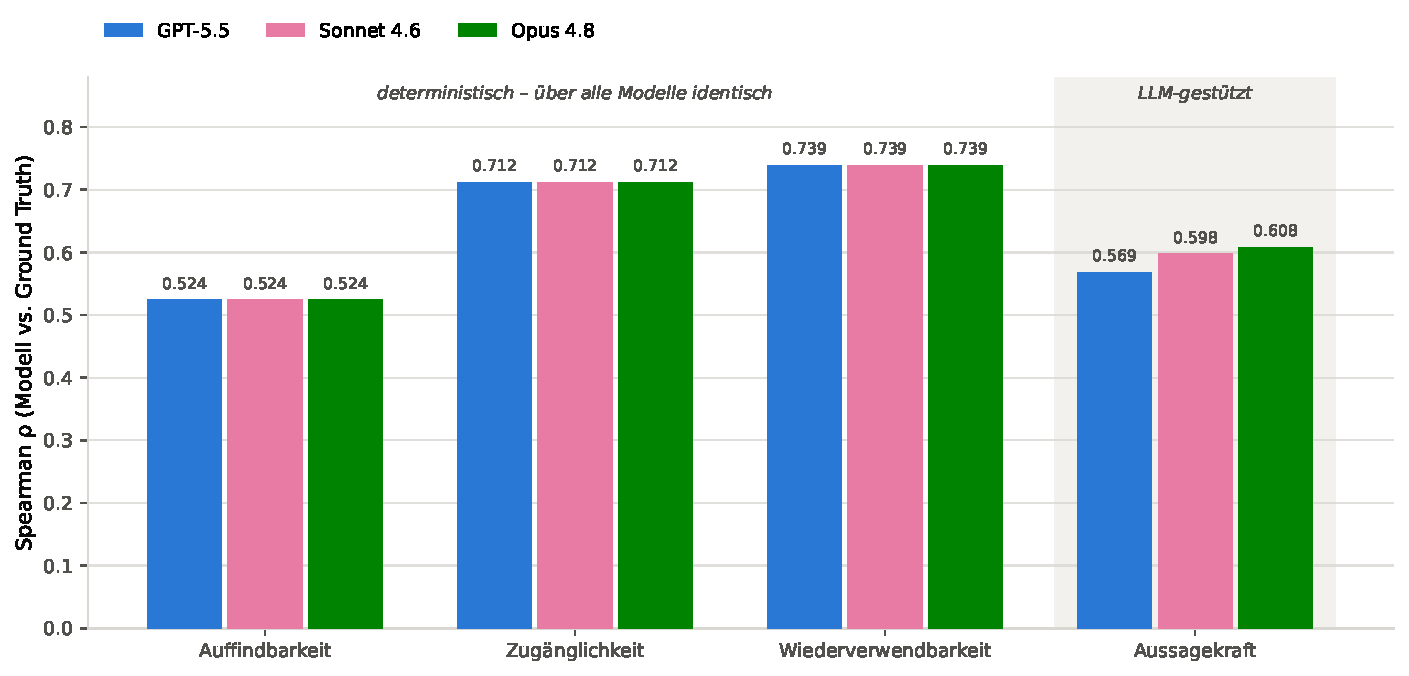
\includegraphics[width=\textwidth]{images/modellauswahl_rho_je_dimension.pdf}
    \captionsetup{justification=centering}
    \caption{Spearman-Rangkorrelation zur Ground Truth je Qualitätsdimension und Sprachmodell (Kernstichprobe, $n = 50$)}
    \label{fig:modellauswahl_dimensionen}
\end{figure}

Der Befund ist eindeutig: In den Dimensionen Auffindbarkeit, Zugänglichkeit und
Wiederverwendbarkeit sind die Werte über alle drei Modelle bitgenau identisch
($\rho = 0{,}524$, $0{,}712$ und $0{,}739$). Die Modellwahl berührt ausschließlich die
Aussagekraft. Für den Vergleich folgt daraus, dass die Aussagekraft die
einzige Dimension ist, auf der die Kandidaten überhaupt sinnvoll gegeneinander zu bewerten
sind. Zudem sind Gesamtkennzahlen für diesen Zweck nur eingeschränkt aussagekräftig,
weil sie den identischen deterministischen Anteil mitmitteln und die tatsächlichen
Unterschiede dadurch verwässern. Die Gesamtwerte werden im Folgenden dennoch berichtet,
da sie die praktische Auswirkung der Modellwahl auf das Endergebnis sichtbar machen.

\subsection{Auswahl des Sprachmodells}
\label{subsec:eval_modellauswahl_auswahl}

Tabelle~\ref{tab:modellauswahl_kennzahlen} stellt die Kandidaten gegenüber. Die
Kennzahlen sind nach der in Abschnitt~\ref{sec:eval_auswertungsverfahren} festgelegten Hierarchie geordnet: zuerst die
Primärmetrik, dann die Kalibrierungsmaße, zuletzt die Urteilsebene als Sekundärmetrik.

\begin{table}[H]
    \centering
    \scriptsize
    \renewcommand{\arraystretch}{1.2}
    \rowcolors{1}{white}{white}
    \begin{tabular}{p{6.2cm}rrr}
    \hline
    \textbf{Kennzahl} & \textbf{GPT-5.5} & \textbf{Opus 4.8} & \textbf{Sonnet 4.6} \\
    \hline
    \multicolumn{4}{l}{\textit{Primärmetrik}} \\
    Spearman $\rho$ Aussagekraft & 0,569 & \textbf{0,608} & 0,598 \\
    Spearman $\rho$ gesamt & 0,765 & \textbf{0,770} & 0,745 \\
    \hline
    \multicolumn{4}{l}{\textit{Kalibrierung}} \\
    MAE (Skala 0--5) & 0,289 & \textbf{0,275} & 0,308 \\
    Bias gesamt & $\mathbf{+0{,}018}$ & $\mathbf{-0{,}018}$ & $-0{,}144$ \\
    Bias Aussagekraft & $\mathbf{-0{,}077}$ & $-0{,}220$ & $-0{,}723$ \\
    \hline
    \multicolumn{4}{l}{\textit{Urteilsebene (Sekundärmetrik)}} \\
    Accuracy & \textbf{0,92} & 0,90 & 0,88 \\
    Cohen $\kappa$ (gewichtet) & \textbf{0,635} & 0,508 & 0,359 \\
    PABAK & \textbf{0,88} & 0,85 & 0,82 \\
    AUC gut-vs-rest & \textbf{0,907} & 0,902 & 0,876 \\
    Als „gut“ erkannt (von 5) & \textbf{3} & 2 & 1 \\
    \hline
    \multicolumn{4}{l}{\textit{Aufwand}} \\
    Kosten je 50 Datensätze (USD) & \textbf{1,79} & 4,10 & 2,02 \\
    \hline
    \end{tabular}
    \captionsetup{justification=centering}
    \caption[Kennzahlenvergleich der Kandidatenmodelle]{Kennzahlenvergleich der Kandidatenmodelle auf der Kernstichprobe ($n = 50$), je ein Lauf pro Modell.}
    \label{tab:modellauswahl_kennzahlen}
\end{table}

\textbf{Opus 4.8} scheidet am Aufwand aus. Das Modell verursacht mit 4,10~USD je
50~Datensätzen etwa doppelt so hohe Kosten wie die beiden anderen Kandidaten, ohne dass
dem ein belastbarer Qualitätsvorsprung gegenüberstünde: Auf der Primärmetrik liegt es
lediglich 0,010 vor Sonnet~4.6 und 0,040 vor GPT-5.5 -- Abstände, die, wie
Abschnitt~\ref{subsec:eval_reproduzierbarkeit} zeigt, kleiner sind als die Schwankung eines einzelnen Modells zwischen
Wiederholungsläufen.

Zwischen \textbf{GPT-5.5} und \textbf{Sonnet 4.6} trennt die Primärmetrik die Kandidaten
nicht. Der Abstand auf der Aussagekraft beträgt in obiger Tabelle 0,029; auf der
Wiederholungsstichprobe, auf der auch die Streuung bestimmt ist ($n = 30$,
Abschnitt~\ref{subsec:eval_reproduzierbarkeit}), sind es 0,028 zugunsten von Sonnet~4.6, während die Streuung desselben
Modells zwischen Wiederholungsläufen dort bei $\sigma = 0{,}023$ liegt. Der Unterschied
entspricht damit dem 1,2-fachen der Streuung, und die Wertebereiche beider Modelle
überlappen einander. Ein Vorsprung dieser Größenordnung ist
auf dieser Stichprobe nicht von Zufallsschwankung zu unterscheiden.

Damit fällt die Entscheidung auf den nachgeordneten Kriterien, und diese weisen
übereinstimmend auf GPT-5.5. Am deutlichsten ist der Befund zur \emph{Kalibrierung}:
Sonnet~4.6 unterschätzt die Aussagekraft systematisch um 0,723 Skalenpunkte, also rund
15\,\% der Skalenbreite, GPT-5.5 dagegen nur um 0,077. Diese Niveauverschiebung ist für
die Rangkorrelation folgenlos -- $\rho$ misst ausschließlich die Reihenfolge -- wirkt
sich auf der Urteilsebene aber unmittelbar aus, weil die Urteilsregel feste Schwellen auf
die gerundeten Dimensionswerte anwendet. Sonnet~4.6 drückt dadurch 19 der 50 Datensätze
unter die konjunktive Sperrklausel „keine Dimension unter 3“ (Ground Truth: 7) und erkennt
in der Folge nur einen der fünf tatsächlich guten Datensätze als „gut“, gegenüber drei bei
GPT-5.5. Für ein Werkzeug, das Datenbereitstellern eine Qualitätsrückmeldung geben soll,
ist eine systematische Abwertung guter Metadaten ein praktisch relevanter Mangel.

Dieser Zusammenhang erklärt zugleich den auf den ersten Blick widersprüchlichen Befund,
dass GPT-5.5 auf der Primärmetrik hinten liegt, auf der Urteilsebene jedoch durchgängig
vorn: Rangkorrelation und Urteilsregel messen unterschiedliche Eigenschaften. Erstere ist
niveaublind und bewertet allein die Reihenfolge, letztere ist niveauempfindlich und
bewertet die absolute Lage relativ zu festen Schwellen. GPT-5.5 bewertet die Datensätze
geringfügig schlechter, verortet sie aber auf dem zutreffenden Niveau. Sonnet~4.6 hingegen ordnet
minimal besser ein, verschiebt jedoch das gesamte Niveau nach unten.

Die Unterschiede auf der Urteilsebene sind allerdings mit Zurückhaltung zu lesen. Die
Konfusionsmatrizen der drei Modelle sind in zwei von drei Zeilen identisch. Der gesamte
Unterschied entsteht in den fünf Datensätzen mit dem Ground-Truth-Urteil „gut“. Aus einer
Differenz von zwei Datensätzen resultiert bereits die $\kappa$-Spanne von 0,635 bis 0,359
--- eine Sensitivität, die den in Abschnitt~\ref{sec:eval_auswertungsverfahren} dargelegten Prävalenzbefund bestätigt und
begründet, warum diese Kennzahlen als Sekundärmetrik geführt werden. Sie stützen die
Entscheidung, tragen sie aber nicht allein.

Gewählt wird daher \textbf{GPT-5.5}. Es ist auf der Primärmetrik von Sonnet~4.6 nicht
unterscheidbar, deutlich besser kalibriert, auf der Urteilsebene durchgängig genauer,
reproduzierbarer (Abschnitt~\ref{subsec:eval_reproduzierbarkeit}) und zugleich das kostengünstigste der drei Modelle.
Alle folgenden Ergebnisse dieses Kapitels beruhen auf diesem Modell.

% Scope: Nachweis, dass das gewaehlte Modell reproduzierbar bewertet. Zwei Funktionen:
% (a) eigenstaendiges Guetekriterium, (b) liefert die Rauschschaetzung, mit der in 5.6.1
% ueberhaupt beurteilt werden kann, ob ein Modellabstand belastbar ist.
%
% Design: drei Wiederholungen mit Sonnet 4.6 auf identischer Teilstichprobe (n=30, alle
% Dateien mit Suffix _02/_03/_04), Auswertung mit Notebook 14. Bewusst nur fuer das
% gewaehlte Modell erhoben -- fuer Opus und GPT liegt keine Streuungsschaetzung vor
% (als Limitation in 5.10 fuehren).
%
% Kennzahlen:
%   Spanne der Run-Mittelwerte     0.0063
%   Ø Standardabweichung je Datei  0.0082
%   MAE zwischen den Laeufen       0.0107
%   Spearman rho zwischen Laeufen  0.9906
%   rho Aussagekraft je Lauf       0.5547 / 0.5818 / 0.5386 -> Spanne 0.0432, sigma 0.0218
%
% Drei Befunde, in dieser Reihenfolge:
%   (1) Validitaetsnachweis der Pipeline: Die drei deterministischen Dimensionen sind
%       ueber alle Laeufe bitgleich. Die gesamte beobachtete Streuung stammt aus der
%       LLM-Bewertung -- alles andere reproduziert exakt.
%   (2) Aufloesungsgrenze: Die Spanne der Run-Mittelwerte (0.0063) ist die Untergrenze,
%       ab der Unterschiede zwischen Konfigurationen oder Modellen ueberhaupt
%       interpretierbar sind. Auf der Aussagekraft betraegt die Streuung von rho zwischen
%       Wiederholungen 0.0432 -- viermal so viel wie der Abstand Sonnet/Opus (0.010).
%       Das ist die quantitative Grundlage fuer den Ausschluss von Opus in 5.6.1.
%   (3) Lokalisierung der Instabilitaet: Die Streuung verteilt sich nicht gleichmaessig,
%       sondern konzentriert sich auf zwei Kriterien -- Kontextuelle Qualifizierer
%       (Statuswechsel bei 47 Prozent der Dateien) und Kohaerenz von Titel und
%       Beschreibung (37 Prozent). Beschreibungs-Qualitaet ist mit 3 Prozent praktisch
%       stabil. Anknuepfungspunkt fuer die Diskussion (Rubrik-Schaerfe) und fuer 5.10.
%
% ABBILDUNG (vorhanden, outputs/model_comparison/plots/): Statuswechsel je Kriterium als
% Balkendiagramm -- zeigt Befund (3) unmittelbar. Die Fehlerbalken-Abbildung
% (Gesamtscore je Datei mit Min-Max-Spanne ueber die Laeufe) belegt Befund (2);
% ihr gezoomtes unteres Panel macht die Streuung ueberhaupt erst sichtbar.
\subsection{Reproduzierbarkeit der Bewertung}
\label{subsec:eval_reproduzierbarkeit}

Da die Bewertung der Aussagekraft auf einem generativen Sprachmodell beruht, ist sie
anders als die übrigen Dimensionen nicht deterministisch. Wie stark die Ergebnisse
zwischen zwei Läufen desselben Modells schwanken, ist deshalb sowohl ein eigenständiges
Gütekriterium als auch die Voraussetzung dafür, Unterschiede zwischen Modellen überhaupt
beurteilen zu können: Ein Abstand, der kleiner ist als die Schwankung eines einzelnen
Modells, trägt keine Aussage.

Erhoben wurden je drei Läufe für GPT-5.5 und Sonnet~4.6 auf einer identischen
Teilstichprobe von 30 Datensätzen. Abbildung~\ref{fig:modellauswahl_wiederholungen} zeigt die
Einzelergebnisse sowie die Spanne je Modell.

\begin{figure}[H]
    \centering
    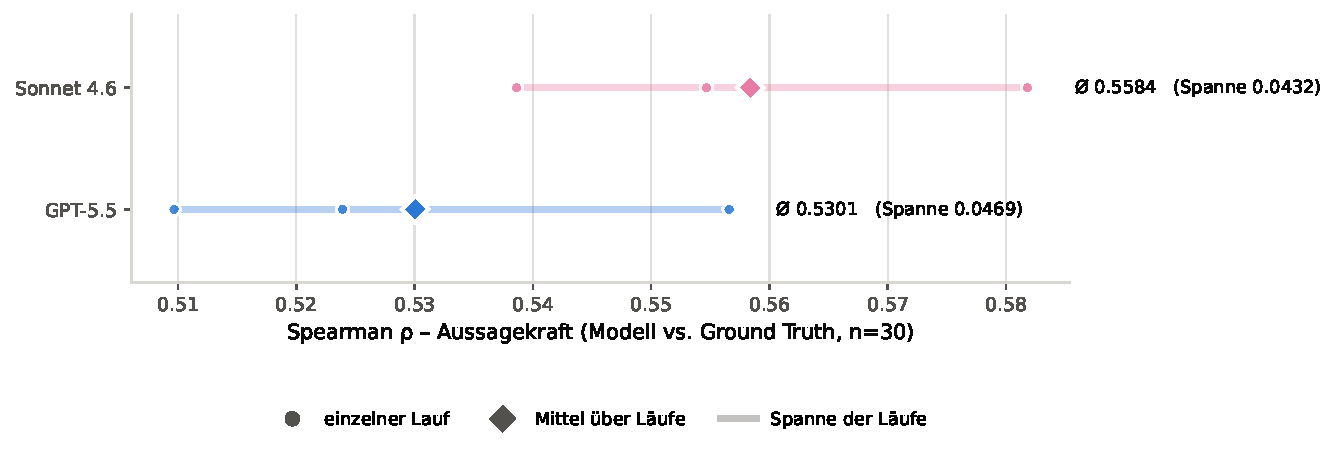
\includegraphics[width=\textwidth]{images/modellauswahl_wiederholungen.pdf}
    \captionsetup{justification=centering}
    \caption[Spearman $\rho$ der Aussagekraft über Wiederholungsläufe]{Spearman $\rho$ der Aussagekraft über je drei Wiederholungsläufe, identische Teilstichprobe ($n = 30$)}
    \label{fig:modellauswahl_wiederholungen}
\end{figure}

Beide Modelle streuen in vergleichbarer Größenordnung: Sonnet~4.6 erreicht im Mittel
$\rho = 0{,}558$ bei einer Spanne von 0,043 ($\sigma = 0{,}022$), GPT-5.5 im Mittel
$\rho = 0{,}530$ bei einer Spanne von 0,047 ($\sigma = 0{,}024$). Dass die Streuung bei
beiden nahezu identisch ausfällt, legt nahe, dass sie weniger eine Eigenschaft des
einzelnen Modells als der Bewertungsaufgabe selbst ist. Die Wertebereiche
überlappen einander deutlich, da der beste Lauf von GPT-5.5 ($\rho = 0{,}557$) über dem
schwächsten von Sonnet~4.6 ($\rho = 0{,}539$) liegt. Dies ist die in Abschnitt~\ref{subsec:eval_modellauswahl_auswahl}
herangezogene Grundlage für die Feststellung, dass die Primärmetrik die beiden Kandidaten
nicht trennt.

Auf der Ebene der Scores, statt der aus ihnen abgeleiteten Rangkorrelation, fällt
der Vergleich klarer aus. Tabelle~\ref{tab:modellauswahl_reproduzierbarkeit} stellt die
Reproduzierbarkeitskennzahlen beider Modelle gegenüber.

\begin{table}[H]
    \centering
    \scriptsize
    \renewcommand{\arraystretch}{1.2}
    \rowcolors{1}{white}{white}
    \begin{tabular}{p{7.4cm}rr}
    \hline
    \textbf{Kennzahl} & \textbf{GPT-5.5} & \textbf{Sonnet 4.6} \\
    \hline
    Spanne der Run-Mittelwerte & \bf{0,0004} & 0,0063 \\
    Ø Standardabweichung je Datensatz & \bf{0,0046} & 0,0082 \\
    Ø Standardabweichung Aussagekraft & \bf{0,0150} & 0,0268 \\
    MAE zwischen zwei Läufen & \bf{0,0059} & 0,0107 \\
    Spearman $\rho$ zwischen zwei Läufen & \bf{0,993} & 0,991 \\
    Höchster Anteil an Statuswechseln je Kriterium & \bf{17\,\%} & 47\,\% \\
    \hline
    \end{tabular}
    \captionsetup{justification=centering}
    \caption[Reproduzierbarkeit über drei Wiederholungsläufe]{Reproduzierbarkeit über je drei Wiederholungsläufe auf identischer Teilstichprobe ($n = 30$)}
    \label{tab:modellauswahl_reproduzierbarkeit}
\end{table}

GPT-5.5 reproduziert seine Bewertungen durchgehend stabiler, auf Ebene der
Run-Mittelwerte um mehr als eine Größenordnung. Dass die Streuung der Rangkorrelation
dennoch minimal höher ausfällt, ist kein Widerspruch: $\rho$ ist eine Rangstatistik, und
bei eng beieinanderliegenden Werten genügen geringe Score-Änderungen, um Ränge zu
vertauschen. Die zugrunde liegenden Scores selbst sind bei GPT-5.5 klar reproduzierbarer.

Drei Befunde sind darüber hinaus festzuhalten. Erstens sind die drei deterministischen
Dimensionen über sämtliche Läufe hinweg bitgenau identisch. Die gesamte beobachtete
Streuung stammt somit aus der LLM-gestützten Bewertung, während die übrige
Verarbeitungskette exakt reproduziert -- ein Validitätsnachweis für die Pipeline als
Ganzes. Zweitens ergibt sich aus der Spanne der Run-Mittelwerte eine Auflösungsgrenze für
alle weiteren Vergleiche: Unterschiede zwischen Konfigurationen oder Modellen, die
kleiner sind als 0,0004 (GPT-5.5), sind nicht interpretierbar. Drittens verteilt sich die
Instabilität nicht gleichmäßig über die Bewertungskriterien, sondern konzentriert sich
auf einzelne von ihnen; bei GPT-5.5 wechselt der diskrete Status im ungünstigsten Fall
bei 17\,\% der Datensätze, bei Sonnet~4.6 dagegen bei 47\,\%. Die betroffenen Kriterien
sind damit als Ansatzpunkt für eine Schärfung der Bewertungsrubrik identifiziert.

\section{Ergebnisse: Prototyp und Ground Truth}
\label{sec:eval_ergebnisse_gt}

Dieser Abschnitt berichtet die in Abschnitt~\ref{sec:eval_auswertungsverfahren} festgelegten Kennzahlen für beide
Stichproben getrennt: zuerst die Kernstichprobe, die die quantitativen Aussagen dieser
Arbeit trägt, dann die Extremfälle, die den Wirkmechanismus per Konstruktion belegen
(Abschnitt~\ref{sec:eval_stichprobe}). Beide Auswertungen verwenden durchgängig GPT-5.5.

\subsection{Kernstichprobe (n=50)}

Primär- und Sekundärmetrik für die Kernstichprobe wurden bereits in
Abschnitt~\ref{subsec:eval_modellauswahl_auswahl} im Rahmen der Modellauswahl vollständig berichtet
(Tabelle~\ref{tab:modellauswahl_kennzahlen}, Spalte GPT-5.5): Spearman $\rho$ gesamt
$= 0{,}765$, Genauigkeit $92\,\%$, gewichtetes $\kappa = 0{,}635$, PABAK $= 0{,}88$,
AUC $= 0{,}907$. Sie bilden zugleich das Hauptergebnis dieses Abschnitts, da GPT-5.5
das für die gesamte übrige Auswertung verwendete Modell ist, und werden hier nicht
wiederholt, sondern um die noch offene Ceiling-Einordnung sowie eine visuelle
Aufbereitung ergänzt.

Abbildung~\ref{fig:gt_kern_dimension} stellt die vier Dimensions-$\rho$ ihrem
jeweiligen Ceiling gegenüber -- dem bei gegebener Ground-Truth-Verteilung maximal
erreichbaren $\rho$ (Abschnitt~\ref{sec:eval_auswertungsverfahren}). Tabelle~\ref{tab:gt_kern_ceiling} listet die
Werte vollständig, einschließlich der tatsächlich genutzten GT-Stufenzahl je
Dimension.

\begin{figure}[H]
    \centering
    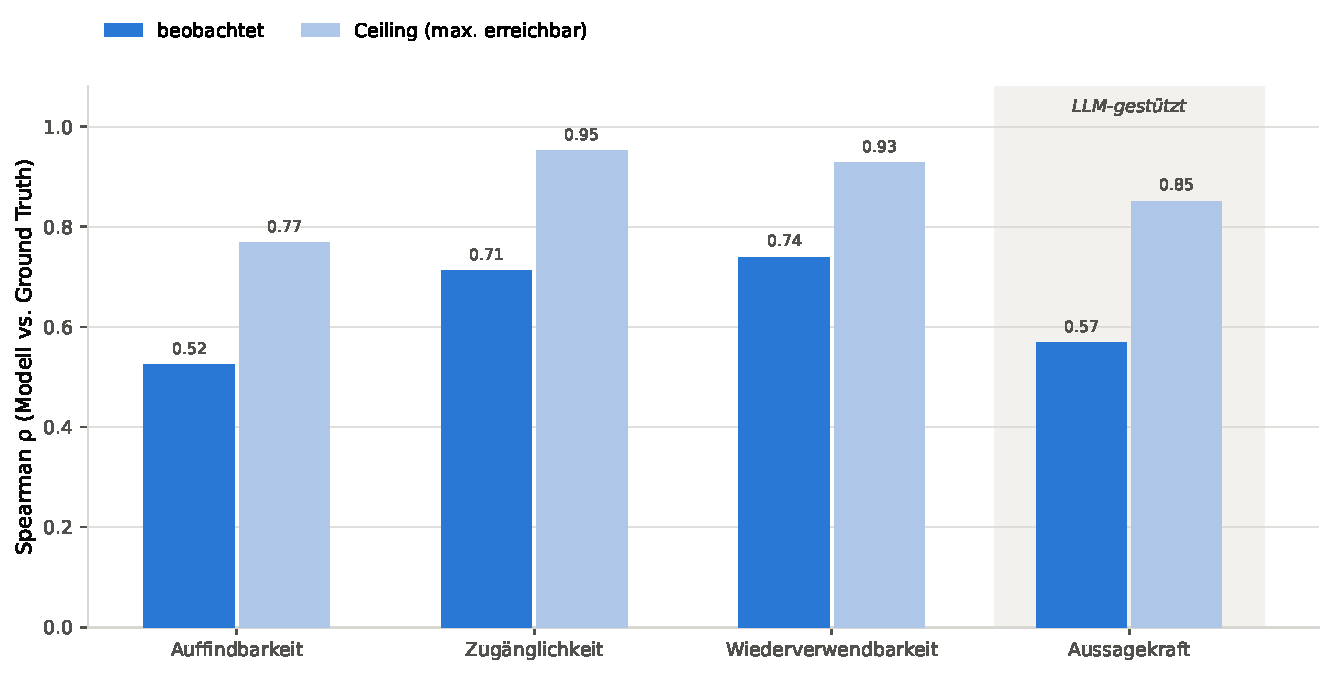
\includegraphics[width=\textwidth]{images/gt_kernstichprobe_rho_dimension.pdf}
    \captionsetup{justification=centering}
    \caption{Spearman $\rho$ je Qualitätsdimension, beobachtet vs. Ceiling (Kernstichprobe, $n=50$)}
    \label{fig:gt_kern_dimension}
\end{figure}

\begin{table}[H]
    \centering
    \scriptsize
    \renewcommand{\arraystretch}{1.2}
    \rowcolors{1}{white}{white}
    \begin{tabular}{lrrrr}
    \hline
    \textbf{Dimension} & \textbf{$\rho$ beobachtet} & \textbf{$\rho$ Ceiling} & \textbf{Anteil} & \textbf{GT-Stufen} \\
    \hline
    Auffindbarkeit & 0,524 & 0,768 & 68,3\,\% & 4 \\
    Zugänglichkeit & 0,712 & 0,952 & 74,8\,\% & 6 \\
    Wiederverwendbarkeit & 0,739 & 0,928 & 79,6\,\% & 6 \\
    Aussagekraft & 0,569 & 0,851 & 66,8\,\% & 4 \\
    \hline
    \end{tabular}
    \captionsetup{justification=centering}
    \caption[Ceiling-Analyse der Kernstichprobe]{Ceiling-Analyse je Dimension (Kernstichprobe, $n=50$): beobachtetes $\rho$, maximal erreichbares $\rho$ bei gegebener GT-Verteilung, Anteil vom Ceiling, Anzahl tatsächlich genutzter GT-Stufen.}
    \label{tab:gt_kern_ceiling}
\end{table}

Dass Auffindbarkeit das niedrigste rohe $\rho$ aufweist, ist damit nur zur Hälfte
ein Skalenartefakt: Das Ceiling liegt mit $0{,}768$ selbst unter dem der übrigen drei
Dimensionen, weil die Ground Truth hier nur vier der sechs Stufen tatsächlich
nutzt. Die verbleibende Lücke zum Ceiling ($68{,}3\,\%$ ausgeschöpft) ist aber real
und kleiner als bei Zugänglichkeit oder Wiederverwendbarkeit ($74{,}8\,\%$ bzw.
$79{,}6\,\%$). Aussagekraft liegt mit $66{,}8\,\%$ auf ähnlichem Niveau wie
Auffindbarkeit -- ein erster Hinweis auf die in Abschnitt~\ref{subsec:eval_gt_extremfaelle} vertiefte Schwäche
dieser Dimension, die auf den Extremfällen deutlich stärker hervortritt.

Die Disattenuationskorrektur (ein Verfahren, das eine gemessene Korrelation um die
Messungenauigkeit beider Seiten bereinigt, um die dahinterliegende ``wahre''
Korrelation zu schätzen) liefert für die Kernstichprobe keinen brauchbaren
Punktschätzer: Cronbachs $\alpha$, ein Maß für die interne Konsistenz der vier
Dimensionswerte, liegt auf der Modellseite bei nur $0{,}294$, weil die vier Dimensionen
absichtlich verschiedene Konstrukte messen; die Korrektur
$r_{\text{latent}} = \rho / \sqrt{\alpha_{GT} \cdot \alpha_{\text{Modell}}}$
überschreitet den zulässigen Wertebereich und wird bei $1{,}0$ gekappt. Dies
bestätigt die in Abschnitt~\ref{sec:eval_auswertungsverfahren} vorab benannte methodische Grenze -- nicht eine
besonders hohe latente Übereinstimmung -- und wird deshalb nicht als Kennzahl
weiterverwendet.

Abbildung~\ref{fig:gt_kern_scatter} zeigt den Gesamtscore-Vergleich nach
GT-Urteil eingefärbt. Die Konfusionsmatrix in Abbildung~\ref{fig:gt_kern_konfusion}
macht sichtbar, dass beide Fehlklassifikationen an der Schwelle
\emph{gut}/\emph{mittel} liegen, keine an der Schwelle \emph{mittel}/\emph{schlecht}
-- der Prototyp verwechselt auf der Kernstichprobe ausschließlich benachbarte
Qualitätsstufen.

\begin{figure}[H]
    \centering
    \begin{minipage}[t]{0.48\textwidth}
        \centering
        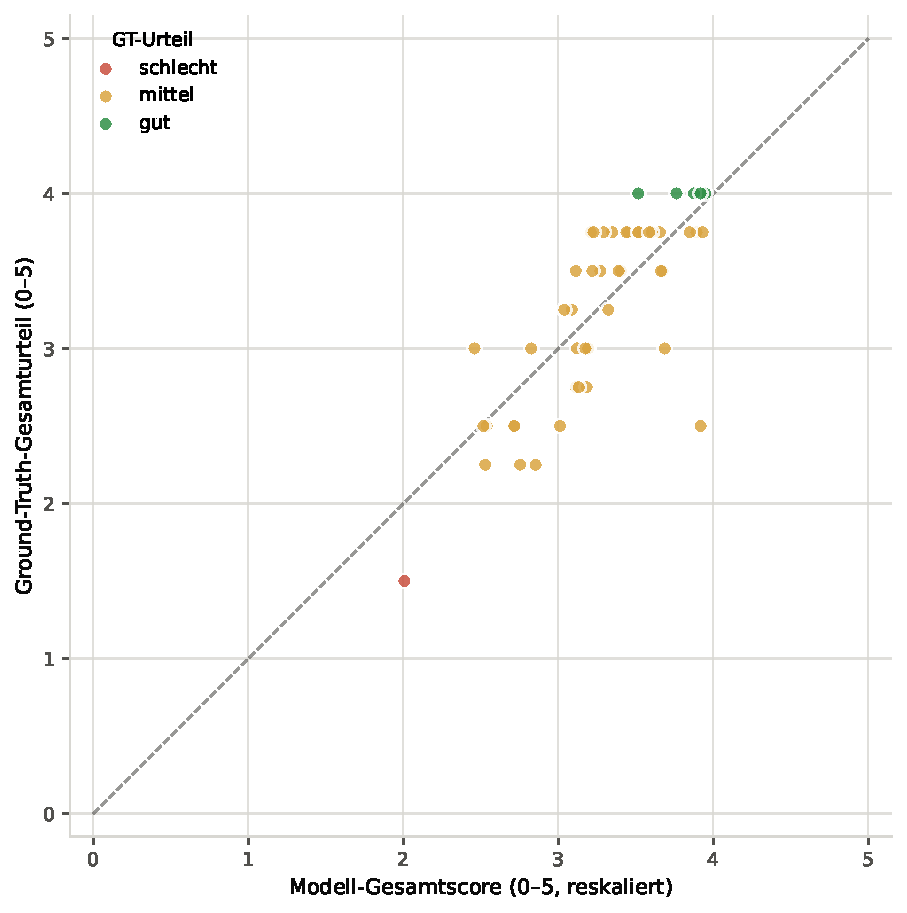
\includegraphics[width=\textwidth]{images/gt_kernstichprobe_scatter.pdf}
        \captionsetup{justification=centering}
        \caption{Modell- vs. Ground-Truth-Gesamturteil, eingefärbt nach GT-Urteil (Kernstichprobe, $n=50$)}
        \label{fig:gt_kern_scatter}
    \end{minipage}
    \hfill
    \begin{minipage}[t]{0.48\textwidth}
        \centering
        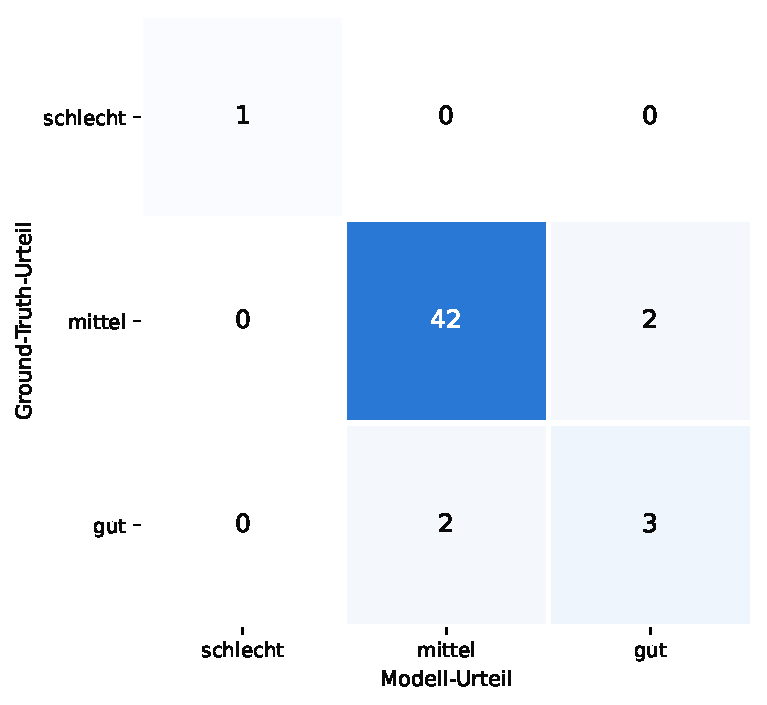
\includegraphics[width=\textwidth]{images/gt_kernstichprobe_konfusionsmatrix.pdf}
        \captionsetup{justification=centering}
        \caption{Konfusionsmatrix des Gesamturteils (Kernstichprobe, $n=50$)}
        \label{fig:gt_kern_konfusion}
    \end{minipage}
\end{figure}

\subsection{Extremfälle (n=20)}
\label{subsec:eval_gt_extremfaelle}

Auf den konstruierten Extremfällen liegt die Gesamtkorrelation mit
$\rho = 0{,}827$ über der Kernstichprobe ($0{,}765$) -- erwartbar, da die Stichprobe
bewusst auf maximale Trennschärfe zwischen guten und schlechten Datensätzen angelegt
ist (Abschnitt~\ref{sec:eval_stichprobe}). Auffindbarkeit und Wiederverwendbarkeit erreichen hier
$90{,}3\,\%$ bzw. $91{,}0\,\%$ ihres jeweiligen Ceilings -- praktisch das bei dieser
Skalengranularität Erreichbare. Zugänglichkeit bleibt mit $\rho = 0{,}713$ nahezu
identisch zur Kernstichprobe ($0{,}712$) und zeigt damit eine über beide Stichproben
stabile Bewertungsgüte (Abbildung~\ref{fig:gt_extrem_dimension},
Tabelle~\ref{tab:gt_extrem_ceiling}).

\begin{figure}[H]
    \centering
    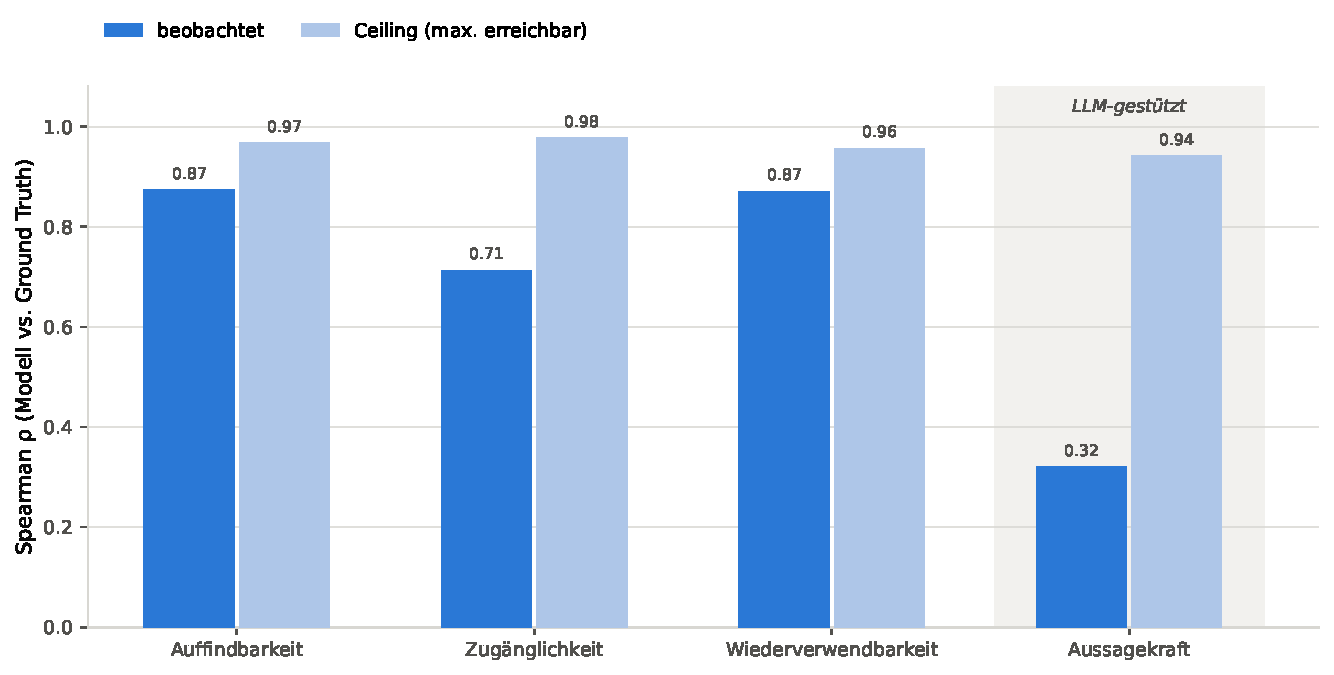
\includegraphics[width=\textwidth]{images/gt_extremfaelle_rho_dimension.pdf}
    \captionsetup{justification=centering}
    \caption{Spearman $\rho$ je Qualitätsdimension, beobachtet vs. Ceiling (Extremfälle, $n=20$)}
    \label{fig:gt_extrem_dimension}
\end{figure}

\begin{table}[H]
    \centering
    \scriptsize
    \renewcommand{\arraystretch}{1.2}
    \rowcolors{1}{white}{white}
    \begin{tabular}{lrrrr}
    \hline
    \textbf{Dimension} & \textbf{$\rho$ beobachtet} & \textbf{$\rho$ Ceiling} & \textbf{Anteil} & \textbf{GT-Stufen} \\
    \hline
    Auffindbarkeit & 0,874 & 0,967 & 90,3\,\% & 5 \\
    Zugänglichkeit & 0,713 & 0,978 & 72,9\,\% & 5 \\
    Wiederverwendbarkeit & 0,872 & 0,957 & 91,0\,\% & 6 \\
    Aussagekraft & 0,321 & 0,942 & 34,1\,\% & 4 \\
    \hline
    \end{tabular}
    \captionsetup{justification=centering}
    \caption[Ceiling-Analyse der Extremfälle]{Ceiling-Analyse je Dimension (Extremfälle, $n=20$).}
    \label{tab:gt_extrem_ceiling}
\end{table}

Aussagekraft fällt dagegen auf $\rho = 0{,}321$ -- deutlich unter den Wert der
Kernstichprobe ($0{,}569$) und mit nur $34{,}1\,\%$ des eigenen Ceilings ($0{,}942$)
der mit Abstand am wenigsten ausgeschöpfte Wert der gesamten Auswertung. Die
Ceiling-Analyse schließt Skalen- oder Stichprobenartefakte hier explizit aus: Selbst
ein perfekt monotones Modell könnte auf dieser Ground-Truth-Verteilung ein $\rho$ von
$0{,}942$ erreichen.

Der Blick auf die Indikatorebene liefert die Erklärung. Die Aussagekraft wird als
ungewichteter Mittelwert aus sechs vom Sprachmodell bewerteten Teilkriterien
gebildet (Abschnitt~\ref{sec:llm_aussagekraft}). Bei dem Metadatensatz
\texttt{bad\_09.rdf} etwa bewertet das Modell die 
Beschreibungsqualität als FAIL ($0{,}15$) mit der
Begründung, die Beschreibung bestehe nur aus dem einzelnen Wort \enquote{Justizblatt}
und erkläre weder Inhalt noch Struktur der Ressource. Die übrigen fünf Teilkriterien
liegen bei $0{,}65$ bis $0{,}95$, sodass der gemittelte Dimensionswert bei $0{,}72$
landet -- ein einzelnes hartes Defizit wird durch fünf unauffällige Werte praktisch
neutralisiert. Bei zehn der zwanzig Extremfälle weicht das resultierende
dreistufige Urteil deshalb vom menschlichen ab (Genauigkeit $50\,\%$), wobei sich die
Fehlklassifikationen auf einen wiederkehrenden Effekt zurückführen lassen: Der
Modell-Aussagekraftswert bewegt sich in praktisch allen Fällen in einem schmalen
Band zwischen $3{,}3$ und $4{,}3$ auf der 0--5-Skala, unabhängig davon, ob die
menschliche Bewertung bei $1$ oder bei $4$ liegt -- etwa bei \texttt{bad\_09.rdf}
selbst (GT $=1$, Modell $=3{,}6$) oder \texttt{good\_02.rdf} (GT $=2$, Modell
$=3{,}8$). Die flache Mittelung komprimiert damit die tatsächliche Streubreite der
Aussagekraft in einen Bereich, der weder erkennbar schlechte noch erkennbar gute
Texte klar heraushebt.

Trotz dieser Schwäche auf Dimensionsebene trennt der Gesamtscore die beiden
Konstruktionsgruppen deutlich: Datensätze mit der Konstruktionsabsicht \emph{gut}
erreichen im Mittel $4{,}06$ (Skala 0--5), solche mit der Absicht \emph{schlecht}
$2{,}10$ (Abbildung~\ref{fig:gt_extrem_trennschaerfe}) -- der Wirkmechanismus
funktioniert also auf Ebene des Gesamturteils, weil die drei übrigen, überwiegend
gut funktionierenden Dimensionen das einzelne schwache Signal im Gesamtmix aus vier
gleich gewichteten Eingangsdimensionen abfedern. Die Disattenuationskorrektur
bestätigt dieses Bild mit einem plausiblen, nicht gekappten Wert von $0{,}959$ bei
Cronbachs $\alpha$ von $0{,}890$ (GT) bzw. $0{,}837$ (Modell) -- anders als bei der
Kernstichprobe korrelieren die vier Dimensionen hier stark genug untereinander, um
eine belastbare Korrektur zuzulassen, weil konstruiert gute bzw. schlechte
Datensätze tendenziell in allen vier Dimensionen gemeinsam ausschlagen.

\begin{figure}[H]
    \centering
    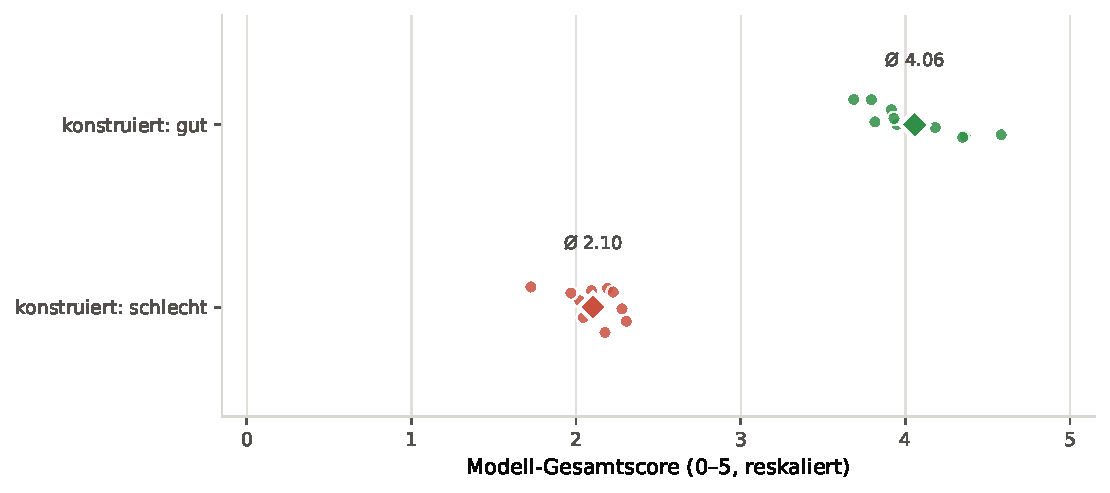
\includegraphics[width=0.85\textwidth]{images/gt_extremfaelle_trennschaerfe.pdf}
    \captionsetup{justification=centering}
    \caption{Modell-Gesamtscore nach Konstruktionsabsicht (Extremfälle, $n=20$)}
    \label{fig:gt_extrem_trennschaerfe}
\end{figure}

Für das Aussagekraftskriterium folgt daraus eine Limitation der
Aggregationslogik, nicht des zugrunde liegenden Sprachmodellurteils selbst: Die
einzelnen Teilkriterien differenzieren sichtbar, der Boxplot in
Abbildung~\ref{fig:mqa_blindheit} zeigt das für dieselbe Kernstichprobe, ihre
ungewichtete Mittelung verschluckt jedoch punktuelle harte Defizite.

% Scope: Entlang A/B/C, also entlang H1/H2. H3 (Korrelation Prototyp<->GT vs. MQA<->GT)
% als Synthese beider Stränge ans Ende des quantitativen Teils. Kernstichprobe und
% Extremfälle getrennt, H3 als gemeinsamer Abschluss.
\section{Ergebnisse: Prototyp und MQA im Vergleich}

Dieser Abschnitt prüft die in Abschnitt~\ref{sec:eval_design} formulierten Hypothesen H1 und H2 anhand
der A/B/C-Klassifikation aus Abschnitt~\ref{sec:eval_mqa_abc} und schließt mit der Triangulation gegen
die Ground Truth (H3), die beide Evidenzstränge dieses Kapitels zusammenführt. Die
MQA-Seite ist rein deterministisch und probe-basiert und daher vom Prototyp-Modell
unabhängig; die Prototyp-Seite verwendet -- wie in Abschnitt~\ref{sec:eval_ergebnisse_gt} -- durchgängig
GPT-5.5.

\subsection{Kernstichprobe (n=50)}

Auf den $9$ Klasse-A-Indikatoren, die im Kern dasselbe prüfen wie eine MQA-Metrik,
stimmen beide Verfahren in $96{,}0\,\%$ der $450$ Datei-Indikator-Paare überein
(Abbildung~\ref{fig:mqa_kern_konvergenz}): $298$-mal sind beide PASS, $134$-mal
beide FAIL. Die verbleibenden $18$ Fälle sind mit $17$ gegen $1$ stark
asymmetrisch verteilt -- MQA vergibt deutlich häufiger einen Pass, den der
Prototyp verweigert, als umgekehrt. Diese hohe Konvergenz bei gleichzeitig
asymmetrischer Restabweichung stützt H1 (konvergente Validität auf äquivalenten
Prüfungen) und deutet zugleich bereits die in H2 erwartete Richtung an.

\begin{figure}[H]
    \centering
    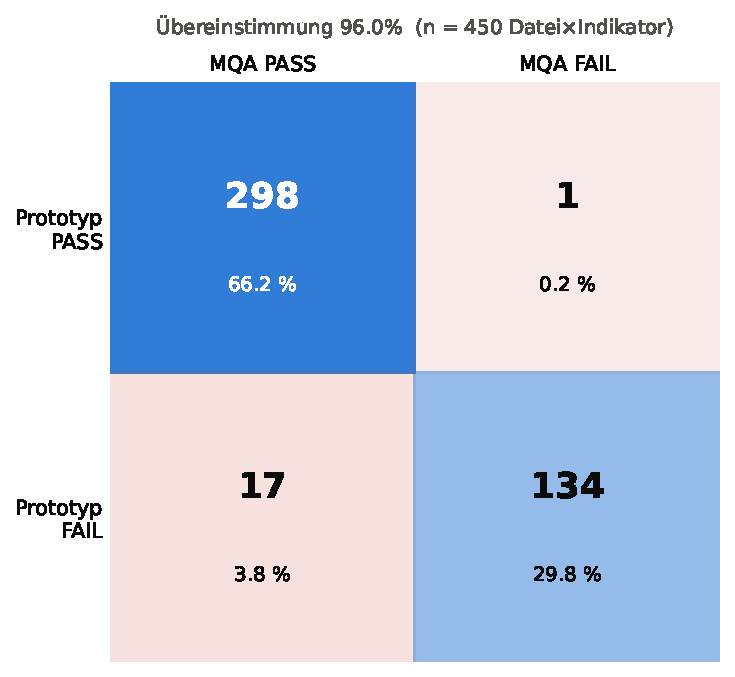
\includegraphics[width=0.55\textwidth]{images/mqa_konvergenz_matrix.pdf}
    \captionsetup{justification=centering}
    \caption{Konvergenz auf Klasse-A-Indikatoren (Kernstichprobe, $n=450$ Datei-Indikator-Paare)}
    \label{fig:mqa_kern_konvergenz}
\end{figure}

Auf den $9$ Klasse-B-Indikatoren, bei denen die MQA Vorhandensein honoriert und
der Prototyp zusätzlich Gültigkeit oder Kongruenz prüft, überschätzt die MQA in
$71$ von $450$ Fällen ($15{,}8\,\%$) die tatsächliche Qualität
(Abbildung~\ref{fig:mqa_kern_ueberschaetzung}). Der stärkste Einzelbefund betrifft
die politische Geokodierung: Bei $56\,\%$ der Datensätze ($28$ von $50$) vergibt
die MQA einen PASS wegen bloßer Existenz, während der Prototyp die tatsächliche Gültigkeit prüft und verweigert. Auf den Klasse-C-Indikatoren, für
die die MQA strukturell keine Metrik besitzt, streut der Prototyp-Score sichtbar
(Abbildung~\ref{fig:mqa_blindheit}): Die Beschreibungsqualität etwa variiert von
$0$ bis $0{,}9$ (Mittelwert $0{,}46$, Standardabweichung $0{,}22$) -- ein Beleg, dass
der Prototyp hier tatsächlich differenziert, statt konstruktiv flach zu bleiben, wie
es die MQA an dieser Stelle per Design ist.

\begin{figure}[H]
    \centering
    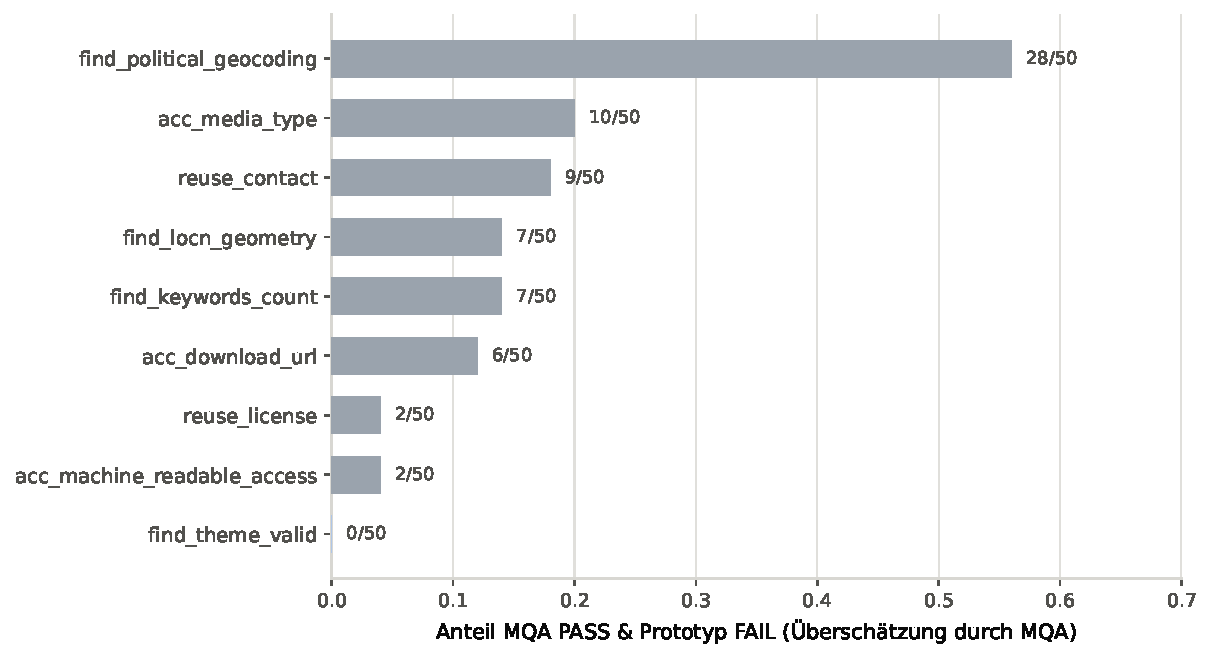
\includegraphics[width=0.85\textwidth]{images/mqa_ueberschaetzung.pdf}
    \captionsetup{justification=centering}
    \caption{Überschätzungsrate je Klasse-B-Indikator: Anteil MQA PASS \& Prototyp FAIL (Kernstichprobe)}
    \label{fig:mqa_kern_ueberschaetzung}
\end{figure}

\begin{figure}[H]
    \centering
    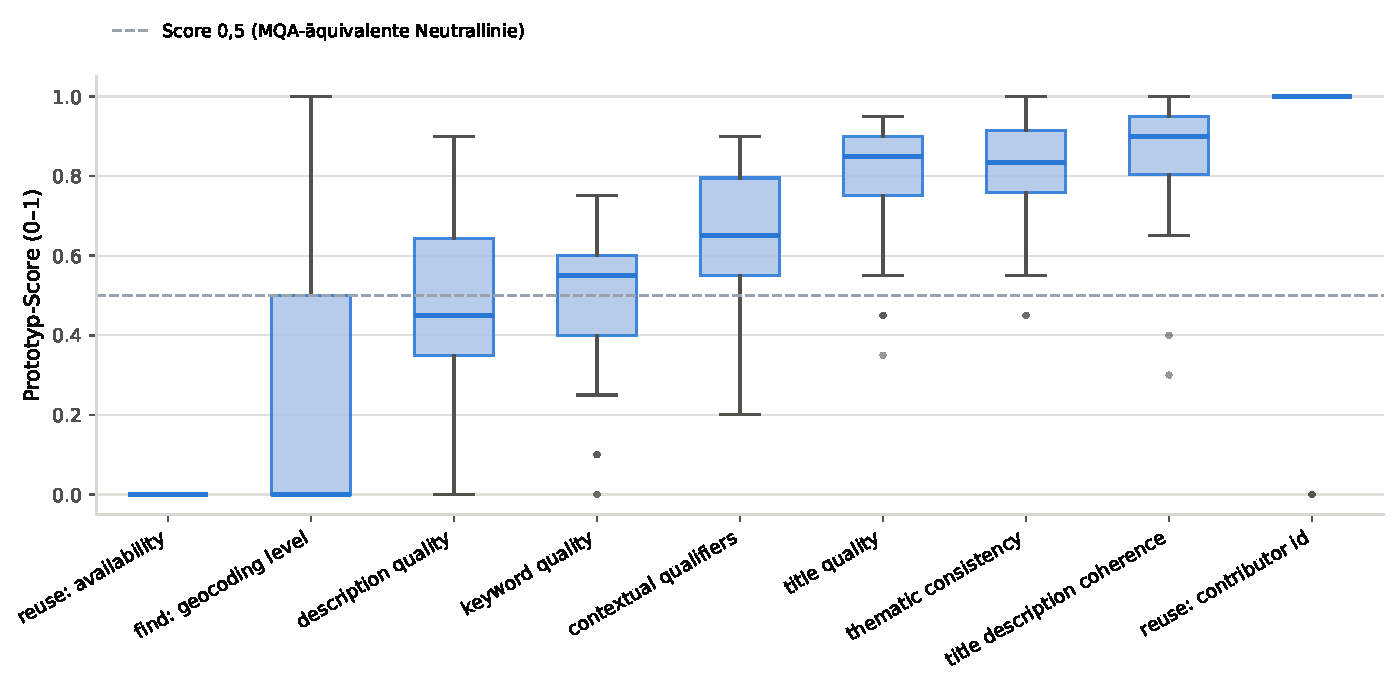
\includegraphics[width=\textwidth]{images/mqa_blindheit_boxplot.pdf}
    \captionsetup{justification=centering}
    \caption{Prototyp-Score-Verteilung auf Klasse-C-Indikatoren, für die die MQA keine Metrik besitzt (Kernstichprobe)}
    \label{fig:mqa_blindheit}
\end{figure}

Auf Ebene der Gesamtscores korrelieren beide Systeme mit $\rho = 0{,}829$ stark
(Abbildung~\ref{fig:mqa_kern_scatter}); die mittlere Differenz beträgt nur
$-0{,}022$ Skalenpunkte zwischen Prototyp und MQA. Diese geringe Niveauverschiebung bei
gleichzeitig hoher Rangkorrelation ist konsistent mit dem Befund aus Klasse~A und~B:
Der Prototyp bewertet überwiegend dieselben Datensätze strenger, nicht andere
Datensätze anders -- eine Rangvertauschung, die $\rho$ senken würde, findet
kaum statt. Die B- und C-Befunde zeigen jedoch, dass diese Ähnlichkeit im Aggregat
reale Messunterschiede auf Indikatorebene überdeckt, die erst im nächsten
Abschnitt (H3) sichtbar werden.

\begin{figure}[H]
    \centering
    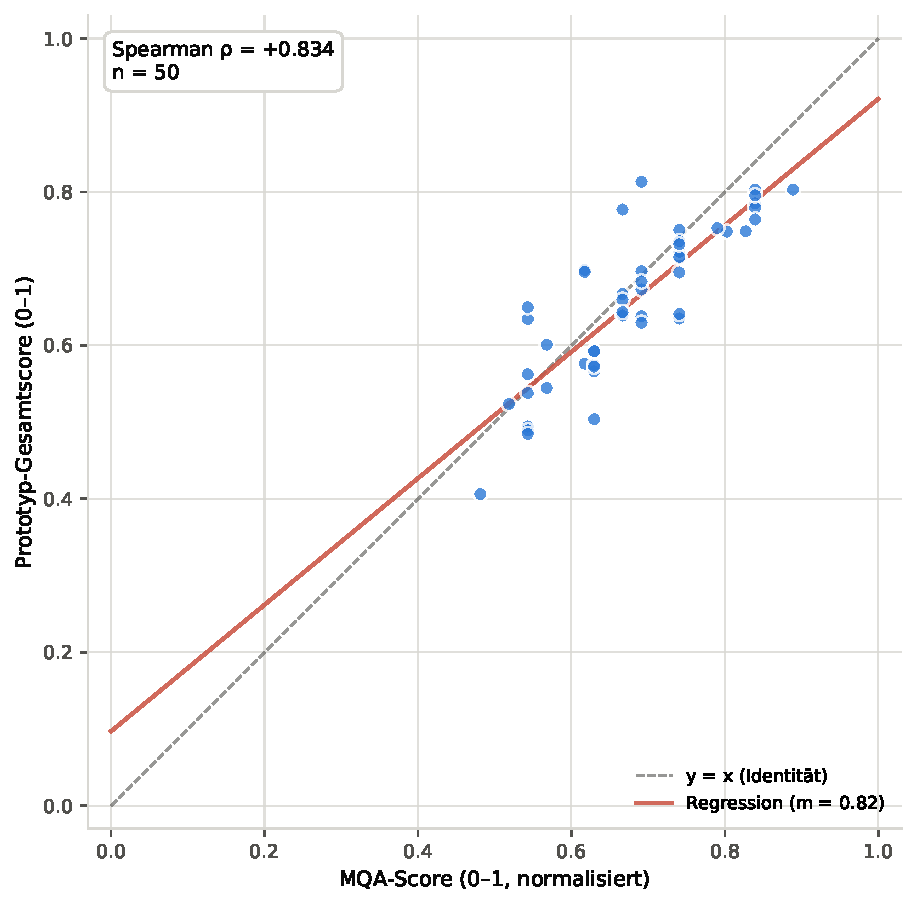
\includegraphics[width=0.62\textwidth]{images/mqa_scatter_gesamt.pdf}
    \captionsetup{justification=centering}
    \caption{Gesamtscore Prototyp vs. MQA (Kernstichprobe, $n=50$)}
    \label{fig:mqa_kern_scatter}
\end{figure}

\subsection{Extremfälle (n=20)}

Auf den Extremfällen fällt die Konvergenz mit $95{,}6\,\%$ ($n=180$) ähnlich hoch
aus wie auf der Kernstichprobe, die Asymmetrie ist hier jedoch vollständig
einseitig (Abbildung~\ref{fig:mqa_extrem_konvergenz}): In $8$ Fällen vergibt die MQA
einen Pass, den der Prototyp verweigert, in keinem einzigen Fall ist es umgekehrt.
Die Überschätzungsrate steigt auf
$20{,}0\,\%$ ($36$ von $180$ Klasse-B-Fällen); dominierend ist hier die Lizenz: Bei
$50\,\%$ der Datensätze ($10$ von $20$) bewertet die MQA die Lizenzangabe als
ausreichend, während der Prototyp sie als ungültig oder unfrei einstuft --
naheliegend, da unter den Extremfällen gezielt Datensätze mit unter anderem fehlerhaften oder
unklaren Lizenzangaben gewählt wurden (Abschnitt~\ref{sec:eval_stichprobe}). Die Klasse-C-Indikatoren
zeigen auch hier durchgängige Streuung, etwa bei der Verfügbarkeitsangabe
(Standardabweichung $0{,}36$) und der Geokodierungsstufe ($0{,}48$). Auf Ebene der
Gesamtscores liegt die Rangkorrelation beider Verfahren bei $\rho = 0{,}820$ und
die mittlere Differenz bei $-0{,}036$ Skalenpunkten -- beides nahe an den Werten der
Kernstichprobe.

Die zugehörigen Abbildungen finden sich vollständig in Anhang~\ref{app:mqa_extremfaelle_abbildungen}.

\subsection{Triangulation gegen die Ground Truth (H3)}

Die bisherigen Befunde belegen, dass Prototyp und MQA unterschiedlich messen (H2),
nicht aber, welches Verfahren näher an der tatsächlichen Qualität liegt. Dafür
werden beide Gesamtscores, unabhängig voneinander, gegen dieselbe
Ground Truth korreliert.

Anders als in Abschnitt~\ref{sec:eval_ergebnisse_gt}, wo je Dimension die
\emph{eigene} Modell-Teilbewertung gegen die gleichnamige GT-Dimension korreliert wird
(Abbildung~\ref{fig:gt_kern_dimension}), steht auf der Prototyp-Seite in diesem Abschnitt
durchgehend der \emph{globale} Gesamtscore. Dieselbe eine Zahl, die auch dem
Scatter in Abbildung~\ref{fig:mqa_kern_scatter} zugrunde liegt. Die Zeile
\enquote{Auffindbarkeit} misst hier also nicht die Güte der
Auffindbarkeits-Teilbewertung selbst, sondern wie gut der \emph{Gesamtscore} die
menschliche Auffindbarkeits-Einschätzung vorhersagt. Diese Wahl ist notwendig, weil
die MQA über keine mit den Prototyp-Dimensionen vergleichbaren Teilscores verfügt und
ein fairer Vergleich beider Systeme deshalb nur auf Ebene des jeweiligen Gesamtscores
möglich ist.

Auf der Kernstichprobe liegt der Prototyp-Gesamtscore
bei fünf von sechs Zielen vorn: gesamt ($0{,}779$ vs. $0{,}740$), ohne Aussagekraft
($0{,}695$ vs. $0{,}671$), Zugänglichkeit ($0{,}591$ vs. $0{,}569$),
Wiederverwendbarkeit ($0{,}457$ vs. $0{,}426$) und Aussagekraft ($0{,}682$ vs.
$0{,}611$) -- Abstände von durchweg $0{,}02$ bis $0{,}07$
(Abbildung~\ref{fig:mqa_kern_triangulation}). Einzige Ausnahme ist die
Auffindbarkeit, auf der die MQA vorn liegt ($0{,}252$ vs. $0{,}134$). Ein naheliegender
Grund liegt in der Gewichtung des Gesamtscores (Abschnitt~\ref{subsec:gewichtung_indikatoren}, Tabelle~\ref{tab:impl_weights}):
Auffindbarkeit geht mit dem niedrigsten Dimensionsgewicht ($1{,}0$ gegenüber $1{,}5$
bis $2{,}0$ bei den übrigen drei Dimensionen) in den Gesamtscore ein und prägt ihn
folglich am wenigsten. Damit ist der Gesamtscore strukturell ein schwächerer
Prädiktor gerade für diese GT-Dimension, unabhängig von der inhaltlichen Prüfgüte der
Auffindbarkeitsindikatoren selbst. Diese liegt laut Abbildung~\ref{fig:gt_kern_dimension} mit
$\rho = 0{,}524$ im Mittelfeld der vier Dimensionen.

Auf den Extremfällen fällt der Befund eindeutiger aus: Der Prototyp liegt hier auf
\emph{allen sechs} Zielen vorn, mit deutlich größeren Abständen als auf der
Kernstichprobe ($+0{,}08$ bis $+0{,}15$. Auch bei der Auffindbarkeit, wo die Kernstichprobe 
die einzige Ausnahme zugunsten der
MQA zeigte ($0{,}755$ vs. $0{,}671$). Das ist plausibel da die Extremfälle gezielt
so selektiert wurden, dass sich Feldpräsenz und tatsächliche Validität auseinanderentwickeln
(Abschnitt~\ref{sec:eval_stichprobe}). Damit genau die Fälle, in denen sich der Vorteil vertiefender Prüfung am
stärksten auszahlen sollte. Abbildung~\ref{fig:mqa_kern_triangulation} und
Abbildung~\ref{fig:mqa_extrem_triangulation} stellen beide Stichproben nebeneinander
dar.

\begin{figure}[H]
    \centering
    \begin{minipage}[t]{0.48\textwidth}
        \centering
        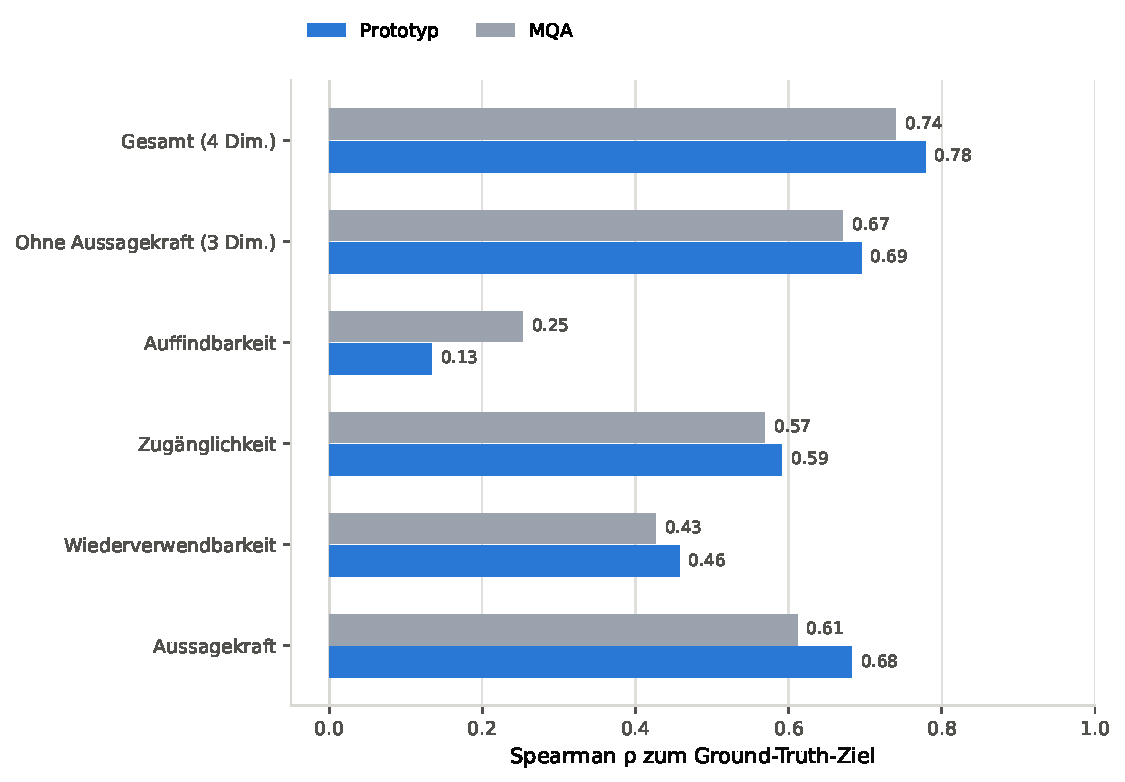
\includegraphics[width=\textwidth]{images/mqa_triangulation_kernstichprobe.pdf}
        \captionsetup{justification=centering}
        \caption{Triangulation gegen die Ground Truth: Spearman $\rho$ von Prototyp und MQA je Zieldimension (Kernstichprobe, $n=50$)}
        \label{fig:mqa_kern_triangulation}
    \end{minipage}
    \hfill
    \begin{minipage}[t]{0.48\textwidth}
        \centering
        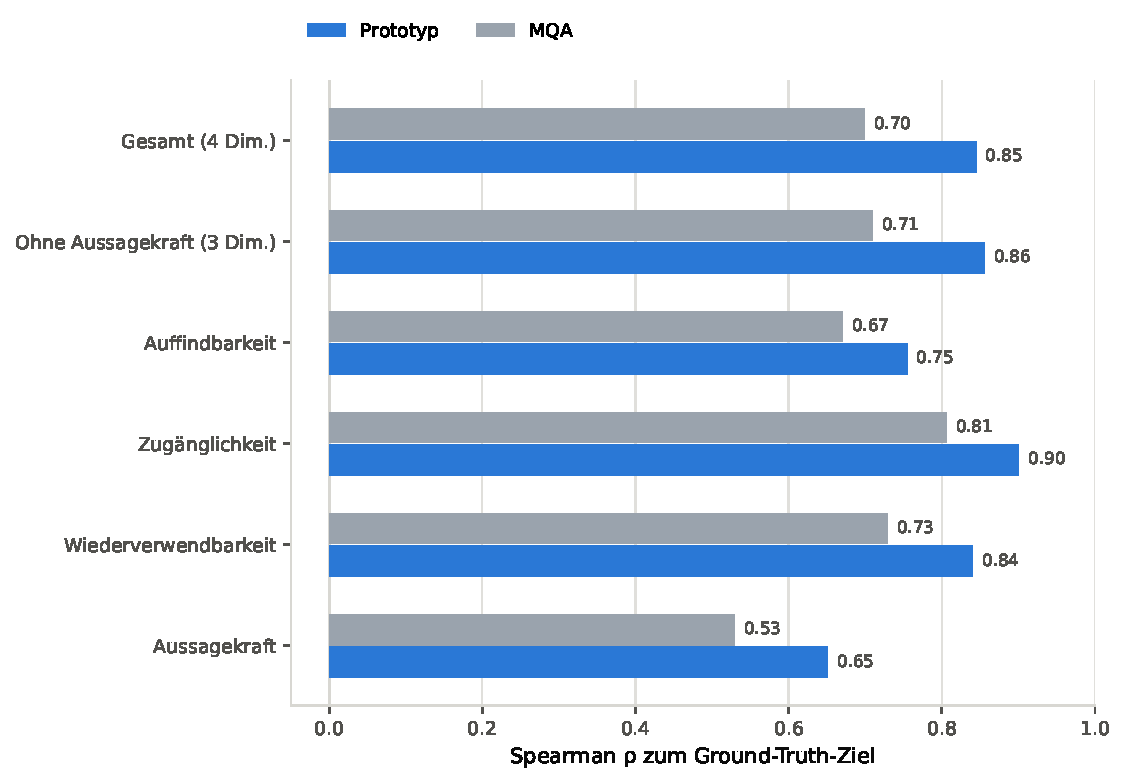
\includegraphics[width=\textwidth]{images/mqa_triangulation_extremfaelle.pdf}
        \captionsetup{justification=centering}
        \caption{Triangulation gegen die Ground Truth: Spearman $\rho$ von Prototyp und MQA je Zieldimension (Extremfälle, $n=20$)}
        \label{fig:mqa_extrem_triangulation}
    \end{minipage}
\end{figure}

Ergänzend zeigt Abbildung~\ref{fig:mqa_extrem_trennschaerfe} beide Systeme auf
derselben Trennschärfe-Darstellung wie Abbildung~\ref{fig:gt_extrem_trennschaerfe},
diesmal auf der gemeinsamen normalisierten 0--1-Skala. Bei den selektiert
schlechten Datensätzen liegen beide Systeme mit $0{,}45$ (MQA) und $0{,}44$
(Prototyp) fast gleichauf. Bei den selektiert guten bewertet die MQA mit
$0{,}88$ etwas großzügiger als der Prototyp mit $0{,}82$. Die absolute Spreizung
zwischen den Gruppen fällt bei der MQA mit $0{,}44$ Punkten sogar geringfügig
größer aus als beim Prototyp ($0{,}38$). MQA ist auf den Extremfällen also
nicht per se weniger trennscharf im Sinne der Score-Spannweite. Der entscheidende
Unterschied liegt nicht in der Breite der Spreizung, sondern in ihrer Richtung
relativ zur menschlichen Bewertung: Die Triangulation zeigt, dass die MQA-Scores
trotz vergleichbarer oder sogar größerer Spreizung schlechter mit der Ground Truth
rangkorrelieren als die des Prototyps. Das ist ein Beleg dafür, dass hohe Streuung allein
noch keine korrekte Rangordnung garantiert.

\begin{figure}[H]
    \centering
    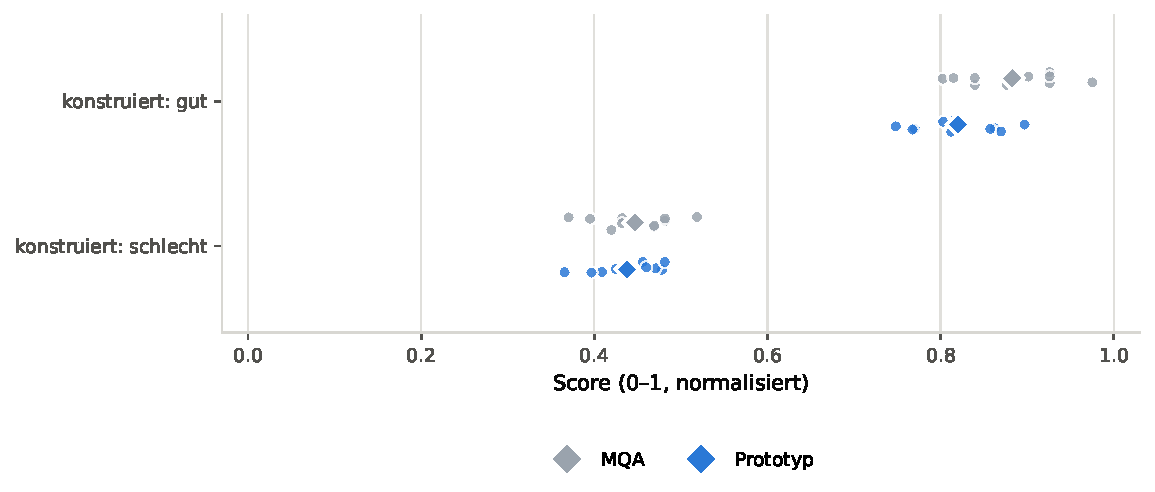
\includegraphics[width=0.85\textwidth]{images/mqa_extremfaelle_trennschaerfe.pdf}
    \captionsetup{justification=centering}
    \caption{Score-Trennschärfe von MQA und Prototyp nach Konstruktionsabsicht (Extremfälle, $n=20$, normalisierte 0--1-Skala)}
    \label{fig:mqa_extrem_trennschaerfe}
\end{figure}

Zusammengenommen stützen die drei Evidenzstränge dieses Kapitels die eingangs
formulierten Hypothesen konsistent: Auf äquivalenten Prüfungen konvergieren
Prototyp und MQA mit über $95\,\%$ Übereinstimmung (H1). Indikatoren, die der Prototyp tiefer
prüft, überschätzt die MQA in $16$ bis $20\,\%$ der Fälle eine Qualität, die nicht
gegeben ist, und differenziert dort, wo die MQA strukturell blind bleibt
(H2). An Stellen wo beide Verfahren divergieren, liegt der Prototyp auf der Kernstichprobe
in fünf von sechs, auf den Extremfällen in allen sechs Zielgrößen näher an der
menschlichen Bewertung (H3). Die einzige Ausnahme, Auffindbarkeit auf der
Kernstichprobe, relativiert diesen Befund, ohne ihn zu widerlegen: Sie zeigt, dass
zusätzliche Prüftiefe nicht in jeder Dimension automatisch mit besserer
menschlicher Übereinstimmung einhergeht.

% Scope: Top-Disagreements aus beiden Vergleichen qualitativ -- wo weicht das Modell vom
% Menschen ab und warum, wo sieht der Prototyp Dinge, die MQA nicht sieht (konkrete
% Datensätze). Hier auch der Screenshot-gestützte Frontend-Walkthrough eines gut/schlecht-
% Falls (Nachvollziehbarkeit des Scorings demonstrativ zeigen).

% @TODO Eventuell wieder einfügen
% \section{Vertiefende Fallanalysen}
% \label{sec:fallanalysen}

% Scope-Ergänzung Frontend (FF5): Die Fallanalysen sind zugleich der Ort, an dem
% die menschenlesbare Aufbereitung (Section~\ref{sec:frontend}) demonstrativ
% gezeigt wird. Vorgehen: an ausgewählten Fällen den Weg vom Gesamtscore über
% den Dimensionsbefund bis zur konkreten Handlungsanweisung nachzeichnen und
% dabei belegen, dass sich jedes Teilergebnis auf eine Prüfregel zurückführen
% lässt. Bewusst ein Walkthrough und keine Nutzerbewertung — die Grenze steht
% in Section~\ref{sec:limitationen_eval}.

% Scope: Nur Limitationen DER EVALUATION (Limitationen des Ansatzes -> Kap. 6/7):
% Einzelbewerter, Stichprobengröße, Skalenartefakte/Attenuation (Disattenuation nur als
% grobe Obergrenze), LLM-Stabilität (Run-zu-Run-MAE), A/B/C-Einstufung als Interpretation,
% Frontend nur demonstrativ statt empirisch mit Nutzern evaluiert.
%
% Ergaenzend zur Modellauswahl (5.6) -- im Text auszuformulieren:
%   - Die Wiederholungsschaetzung beruht auf drei Laeufen je Modell auf der
%     Teilstichprobe n=30, waehrend der Kennzahlenvergleich auf n=50 gerechnet ist.
%     Die Aussage "Abstand innerhalb der Streuung" ist ein Groessenordnungsvergleich
%     (1,2-fache Streuung, ueberlappende Wertebereiche), kein Signifikanztest; bei
%     drei Laeufen je Modell ist sigma selbst nur grob geschaetzt.
%   - Fuer Opus 4.8 existiert nur ein Lauf; seine Streuung ist unbekannt. Der
%     Ausschluss stuetzt sich daher primaer auf die Kosten, nicht auf die Streuung.
%   - Je Modell wurde nur ein Prompt bzw. eine Rubrikfassung getestet; die Ergebnisse
%     sind Aussagen ueber die Kombination Modell + Prompt, nicht ueber das Modell allein.
%   - Auch das gewaehlte Modell unterschaetzt die Aussagekraft leicht (Bias -0,077).
%     Eine Kalibrierung der Rubrik-Anker wurde nicht vorgenommen und bleibt offen.
\section{Limitationen der Evaluation}
\label{sec:limitationen_eval}


% ===========================================================================
% Gliederungsprinzip dieses Kapitels
% ---------------------------------------------------------------------------
% Die Diskussion folgt nicht den Forschungsfragen, sondern der Erkenntniskette
% der Kapitel 2 bis 6. Grund: FF1-FF5 werden über vier Kapitel hinweg
% beantwortet, und die Evaluation prüft H1-H3 zum Messinstrument, nicht die
% Forschungsfragen. Eine FF-getaktete Diskussion würde daher entweder das Fazit
% vorwegnehmen oder redundant werden.
%
% Arbeitsteilung mit dem Fazit:
%   Diskussion  -> Achse Erkenntniskette. Bewertet die Metrik: was hat
%                  getragen, was nicht, warum.
%   Fazit       -> Achse Forschungsfragen. Beantwortet knapp, was gefragt war,
%                  mit Rückverweis in die Diskussion.
%
% Jeder Abschnitt folgt demselben Muster: Befund -> Mechanismus (warum ist das
% so) -> Rückbindung an Literatur/Interviews -> Implikation. Die Abschnitte
% sollen quervernetzt sein, nicht nebeneinanderstehen: Abschnitt zur Evaluation
% greift auf Literatur, Konzept und Interviews zurück.
% ===========================================================================
\chapter{Diskussion}
\label{sec:chapter_07}

% Scope: Rahmen, ca. 1 Seite. Die Verengungslogik der Arbeit explizit machen:
% Literatur (breit, nicht operationalisierbar) -> Interviews (praxisrelevant,
% teils nicht messbar) -> Konzept (formale Indikatoren) -> Prototyp (was
% implementierbar war) -> Evaluation (was nachweislich trägt). Jede Stufe wirft
% weg, was die nächste nicht tragen kann; diese Verengung zu begründen statt
% nur zu vollziehen ist der Zweck dieses Kapitels. Hier auch die Leserichtung
% ansagen und die Abgrenzung zum Fazit benennen.
\section{Verengung von der Theorie zur messbaren Metrik}
\label{sec:disk_verengung}

% Scope: Diskussion von Kapitel~\ref{sec:chapter_02}. Nicht die Ansätze erneut
% referieren (das steht dort), sondern bewerten, was übernommen wurde und was
% nicht:
%   - Wang/Strong, ISO 25012, FAIR haben gerahmt, aber nichts Prüfbares
%     geliefert. Warum ist das kein Mangel, sondern erwartbar?
%   - Zaveri et al. machen Qualitätsaspekte sichtbar, die nicht alle prüfbar
%     waren. Welche konkret, und woran scheiterte es (Kontextwissen, externe
%     Referenzdaten, manuelle Bewertung)?
%   - ISO 19157 / Nogueras-Iso: welcher Beitrag blieb, welcher nicht?
%   - MQA wurde übernommen UND als Baseline gegen den Prototyp gestellt. Die in
%     Abschnitt~\ref{sec:bewertungsluecke} behauptete Reduktionsproblematik ist
%     damit in Kapitel~6 gemessen statt nur postuliert.
% Belegbar machen über die Spalte "Herleitung" der Indikatortabellen
% (Tabelle~\ref{tab:herleitungssignale}): Wie viele Indikatoren stammen aus
% welcher Quelle? Das ist ein prüfbares Argument statt einer Behauptung.
\section{Bestehende Ansätze: Übernommenes und Verworfenes}
\label{sec:disk_grundlagen}

% Scope: Diskussion von Kapitel~\ref{sec:chapter_03}. Die fünf Modellan-
% forderungen aus der Interviewauswertung sind unterschiedlich weit gekommen.
% Ehrlich aufschlüsseln:
%   - gut umgesetzt: semantische Aussagekraft, technische Nutzbarkeit
%   - schwächer: Metadaten-Daten-Kongruenz, kontextsensitive Gewichtung
%     (konzeptionell klar, in der Operationalisierung deutlich reduziert)
% Zentrale Frage der Betreuung: Welcher Expertengedanke hat sich als nicht
% operationalisierbar erwiesen, und WORAN? Das ist der Teil, der geprüft wird.
% Ebenfalls hierher: die drei Zielgruppen aus Abschnitt~\ref{subsec:zielgruppen}.
% Die Metrik bedient Datenbereitstellende gut, Portalbetreibende und
% Datennutzende nur mittelbar -- eine Folge der Bewertungsebene (Einzeldatensatz),
% nicht ein Versäumnis der Umsetzung.
\section{Expertenanforderungen zwischen Anspruch und Messbarkeit}
\label{sec:disk_experten}

% Scope: Abgleich zwischen dem konzeptionellen Messmodell
% (Abschnitt~\ref{sec:messmodell}) und seiner Implementierung
% (Abschnitt~\ref{sec:einzelindikatoren}). Nicht die Umsetzung wiederholen,
% sondern die Entwurfsentscheidungen bewerten:
%   - Was hat getragen: Ergebnisstufen, ternäre vs. graduelle Indikatoren,
%     Aggregation über Distributionen, Malus-Prinzip, Nicht-Anwendbarkeit.
%   - Was hat gehakt: welche Indikatoren mussten beim Implementieren
%     nachgeschärft werden, wo weicht die Implementierung vom Konzept ab?
%   - Der interessanteste Fall ist die LLM-gestützte Aussagekraftsbewertung
%     (Abschnitt~\ref{sec:llm_aussagekraft}): Ein nicht deterministisches
%     Verfahren wird in eine deterministisch gedachte Metrik eingebaut. Was
%     kostet das, was bringt es, und was folgt aus Ein-Aufruf-Architektur,
%     strukturierter Ausgabe und Temperatur-/Seed-Konfiguration?
\section{Vom konzeptionellen Messmodell zur Implementierung}
\label{sec:disk_konzept_prototyp}

% Scope: Diskussion von Kapitel~6. NICHT die Kennzahlen wiederholen, sondern:
% Was hat die Evaluation über die Metrik gelehrt, das aus Konzept und
% Implementierung allein nicht ableitbar war? Kandidaten:
%   - Deckenprüfung am Referenzdatensatz (Abschnitt~\ref{subsec:deckenpruefung}):
%     misst das Instrument nach oben überhaupt trennscharf?
%   - Modellauswahl (Abschnitt~\ref{sec:eval_modellauswahl}) und
%     Reproduzierbarkeit (Abschnitt~\ref{subsec:eval_reproduzierbarkeit}): die
%     Metrik ist modellabhängig. Das ist eine Eigenschaft der Metrik, nicht nur
%     der Implementierung.
%   - Extremfälle: belegen den Wirkmechanismus per Konstruktion -- was heißt das
%     für die externe Validität, gegenüber der Kernstichprobe?
%   - H3 aus Abschnitt~\ref{sec:eval_design} trägt die eigentliche
%     Überlegenheitsaussage; H2 allein belegt nur andersartiges, nicht besseres
%     Messen.
%   - Ground Truth: Spearman rho statt kappa als Primärmetrik ist eine
%     methodische Entscheidung und gehört begründet.
% Quervernetzung: Rückgriff auf Abschnitt~\ref{sec:disk_grundlagen} (die
% MQA-Reduktionsthese ist jetzt gemessen), \ref{sec:disk_konzept_prototyp} (der
% LLM-Determinismus zeigt sich in der Reproduzierbarkeitsprüfung) und
% \ref{sec:disk_experten} (welche Expertenanforderung hat sich in der Messung
% als tragfähig erwiesen).
\section{Was die Evaluation über die Metrik zeigt}
\label{sec:disk_evaluation}

% Scope: Diskussionsteil zu FF5. Nicht die Umsetzung wiederholen (das steht in
% Section~\ref{sec:frontend}), sondern die Tragweite der Entwurfsentscheidungen
% einordnen: Was gewinnt ein Bewertungsverfahren dadurch, dass es Befund und
% Handlungsanweisung statt einer Punktzahl ausgibt? Was folgt aus der Trennung
% von Metadaten- und Bewertungsebene für die Anschlussfähigkeit an ein
% bestehendes Portal? Und wo endet die Aussagekraft ohne empirische Prüfung
% mit Datenbereitstellern?
% Ergänzend: Dass FF5 als einzige Teilfrage ohne empirische Prüfung bleibt, ist
% selbst ein Befund und gehört ausgesprochen.
\section{Nachvollziehbarkeit als Gestaltungsziel des Qualitätsreportings}
\label{sec:disk_nachvollziehbarkeit}

% Scope: Abgrenzung zu Abschnitt~\ref{sec:limitationen_eval}. Dort steht, was
% das EXPERIMENT nicht zeigen kann; hier steht, was die METRIK nicht kann.
% Wechselseitig verweisen, damit die Trennung sichtbar bleibt. Dreiteilung über
% \paragraph{}:
%   - Konzeptuelle Grenzen: was an Metadatenqualität grundsätzlich nicht
%     automatisiert prüfbar ist (Kontextabhängigkeit, Zweckbindung,
%     fachliche Beurteilung).
%   - Methodische Grenzen der Metrik: Gewichtung ist gesetzt und nicht empirisch
%     validiert; Ground Truth von wenigen Ratern; Domänen- und
%     Portalabhängigkeit der Indikatorauswahl.
%   - Technische Grenzen: LLM-Abhängigkeit und Modellversionierung,
%     Reproduzierbarkeit, Laufzeit und Kosten im Portalbetrieb.
\section{Grenzen der Metrik}
\label{sec:disk_grenzen}


\chapter{Fazit und Ausblick}
\label{sec:chapter_08}

% Scope: 3-4 Absätze narrativ, keine Wiederholung von Kennzahlen. Was war das
% Ziel, was ist entstanden, was trägt es. Die Begründungen stehen in
% Kapitel~\ref{sec:chapter_07} und werden hier nicht wiederholt.
\section{Zusammenfassung der zentralen Ergebnisse}

% Scope: FF1-FF5 aus Abschnitt~\ref{sec:forschungsfragen} als fettgesetzte
% Frage-Antwort-Blöcke, ca. ein Absatz je Frage. Diese Blöcke dürfen kurz
% bleiben, WEIL die Diskussion die Begründung bereits geliefert hat; jede
% Antwort verweist in den zuständigen Diskussionsabschnitt:
%   FF1 (Übertragbarkeit bestehender Ansätze) -> \ref{sec:disk_grundlagen}
%   FF2 (relevante Dimensionen und Indikatoren) -> \ref{sec:disk_experten}
%   FF3 (ergänzende kontext-/semantikbezogene Prüfungen)
%        -> \ref{sec:disk_konzept_prototyp}, \ref{sec:disk_grenzen}
%   FF4 (Konzeption und Operationalisierung)
%        -> \ref{sec:disk_konzept_prototyp}, \ref{sec:disk_evaluation}
%   FF5 (menschenlesbares Qualitätsreporting)
%        -> \ref{sec:disk_nachvollziehbarkeit}
\section{Beantwortung der Forschungsfragen}

% Kein eigener Limitationen-Abschnitt im Fazit. Die Limitationen sind auf zwei
% Stellen aufgeteilt, die sich sauber trennen lassen:
%   Abschnitt~\ref{sec:limitationen_eval} -> was das Experiment nicht zeigen kann
%   Abschnitt~\ref{sec:disk_grenzen}      -> was die Metrik nicht kann
% Eine dritte Zusammenfassung hier wäre eine Dopplung ohne eigenen Beitrag.

% Scope: Jeder Punkt hier soll aus einer Grenze in Abschnitt~\ref{sec:disk_grenzen}
% folgen und nicht frei danebenstehen. Also je Forschungsbedarf angeben, welche
% Grenze ihn motiviert (z.B. empirische Validierung der Gewichtung, Nutzerstudie
% zum Reporting mit Datenbereitstellenden, Ausweitung der Ground Truth,
% Portalbetrieb über die Zeit statt Einzeldatensatz).
\section{Weiterer Forschungs- und Entwicklungsbedarf}

%% Use letters for the chapter numbers of the appendices.
\appendix

%\input{appendix-a}

\glsaddall
\printglossary[type=\acronymtype, title=Abkürzungsverzeichnis, nonumberlist]
\addcontentsline{toc}{chapter}{Abkürzungsverzeichnis}
\clearpage
\listoffigures
\addcontentsline{toc}{chapter}{\listfigurename}
\listoftables
\addcontentsline{toc}{chapter}{\listtablename}
\clearpage
\printbibliography[heading=bibintoc]

\newpage

\appendix

\chapter{Interviewleitfaden}
\label{app:interviewleitfaden}

\includepdf[pages=-]{appendix/interviewleitfaden.pdf}

\chapter{Induktiv entwicklete Unterkategorien}
\label{app:unterkategorien}
\begin{table}[H]
\rowcolors{1}{white}{white}
\centering
\tiny
\renewcommand{\arraystretch}{0.8}
\label{tab:unterkategorien}

\begin{tabular}{p{1cm} p{8.8cm} p{2.5cm}}
\toprule
\textbf{Code} & \textbf{induktive Unterkategorie} & \textbf{Belegstellen} \\
\midrule

\multicolumn{3}{l}{\textbf{K1 Qualitätsverständnis und ideale Metadaten}} \\
\midrule
K1.1 & Mindestvalidität und Best Practice & I1\_002--I1\_004 \\ \hline
K1.2 & Qualität statt Quantität & I3\_002--I3\_003 \\ \hline
K1.3 & Metadaten als Inhalts- und Nutzungsvorschau & I3\_005 \\ \hline
K1.4 & semantischer Graph als Idealform & I2\_003--I2\_006 \\
\midrule

\multicolumn{3}{l}{\textbf{K2 Vollständigkeit, Reichhaltigkeit und Feldrelevanz}} \\
\midrule
K2.1 & relative Vollständigkeit & I2\_026 \\ \hline
K2.2 & empfohlene Felder über Pflichtfelder hinaus & I1\_007--I1\_010; I3\_013 \\ \hline
K2.3 & fachlich vorhandene Informationen übernehmen & I2\_004--I2\_005 \\ \hline
K2.4 & relevante Felder statt maximale Feldanzahl & I3\_002--I3\_003 \\
\midrule

\multicolumn{3}{l}{\textbf{K3 Formale und syntaktische Qualität}} \\
\midrule
K3.1 & DCAT-AP.de-Mindestvalidität & I1\_002 \\ \hline
K3.2 & SHACL-Konformität als Basisdimension & I1\_027--I1\_029; I3\_015 \\ \hline
K3.3 & URI- und Vokabularkorrektheit & I3\_003; I3\_018 \\ \hline
K3.4 & Trennung von fehlendem Feld und syntaktischem Fehler & I3\_017 \\ \hline
K3.5 & XML/RDF-Validität und Datentypprüfung & I3\_018 \\
\midrule

\multicolumn{3}{l}{\textbf{K4 Semantische und inhaltliche Qualität}} \\
\midrule
K4.1 & nichtssagende oder zu kurze Titel & I2\_008 \\ \hline
K4.2 & Titel-Beschreibung-Redundanz & I2\_008 \\ \hline
K4.3 & regionale Begriffe und Fachsprache & I2\_009--I2\_010; I1\_043 \\ \hline
K4.4 & verständliche und erklärende Beschreibung & I2\_027; I3\_005 \\ \hline
K4.5 & inhaltliche Widersprüche zwischen Metadatenfeldern & I2\_011; I2\_047 \\ \hline
K4.6 & Keywords, Themenfeld und Kategorie als semantische Prüffelder & I1\_041; I3\_028 \\
\midrule

\multicolumn{3}{l}{\textbf{K5 Technische Zugänglichkeit, Aktualität und Nutzbarkeit}} \\
\midrule
K5.1 & Dead Links und Linkrot & I1\_015; I2\_011 \\ \hline
K5.2 & funktionierende Distributions-, Download- und Servicelinks & I1\_015; I2\_028 \\ \hline
K5.3 & Aktualität und Harvesting-Zeitpunkt & I1\_019; I1\_024--I1\_025 \\ \hline
K5.4 & Maschinenlesbarkeit und nicht-proprietäre Formate & I3\_021 \\
\midrule

\multicolumn{3}{l}{\textbf{K6 Interoperabilität und Linked-Data-Qualität}} \\
\midrule
K6.1 & URI statt Literal & I1\_020--I1\_022 \\ \hline
K6.2 & externe Referenzsysteme, Wikidata und GND & I2\_005; I1\_022 \\ \hline
K6.3 & kontrollierte Vokabulare und Thesauri & I2\_005; I2\_055; I3\_018 \\ \hline
K6.4 & Querverbindungen zwischen vergleichbaren Datensätzen & I2\_006; I2\_056 \\ \hline
K6.5 & Organisationsgraph und Vermeidung von Blank Nodes & I2\_029 \\
\midrule

\multicolumn{3}{l}{\textbf{K7 Kontextsensitivität und Fit for Purpose}} \\
\midrule
K7.1 & domänenspezifische Feldrelevanz & I1\_006; I1\_009--I1\_010 \\ \hline
K7.2 & Geodaten und Normierungsgrad & I1\_031--I1\_033; I3\_022 \\ \hline
K7.3 & föderale Vergleichbarkeit & I1\_040 \\ \hline
K7.4 & Stakeholder-spezifische Qualitätsfragen & I1\_047--I1\_049 \\ \hline
K7.5 & unterschiedliche Perspektiven von Bereitstellenden und Nutzenden & I1\_019 \\
\midrule

\multicolumn{3}{l}{\textbf{K8 Rohdatenbezug und Metadaten-Daten-Kongruenz}} \\
\midrule
K8.1 & Formatkongruenz zwischen Metadaten und Ressource & I2\_045; I3\_020 \\ \hline
K8.2 & Serviceverhalten und tatsächliche Nutzbarkeit & I2\_046 \\ \hline
K8.3 & Dateninhalt gegen Titel und Beschreibung prüfen & I2\_047 \\ \hline
K8.4 & Bounding Box und Flächendeckung aus Daten ableiten & I2\_013; I2\_059 \\ \hline
K8.5 & fachliche Grenzen der Rohdatenbewertung & I3\_022 \\
\midrule

\multicolumn{3}{l}{\textbf{K9 Scoring, Gewichtung, Reporting und Verbesserungshinweise}} \\
\midrule
K9.1 & wissenschaftlich begründete Metriken & I2\_021--I2\_024 \\ \hline
K9.2 & SHACL als Teildimension statt Gesamtscore & I1\_028--I1\_029 \\ \hline
K9.3 & Teil-Scores zur Problemlokalisierung & I2\_039--I2\_040 \\ \hline
K9.4 & Ranking als Verbesserungsanreiz & I2\_034--I2\_037 \\ \hline
K9.5 & verständliche Fehlermeldungen und Handlungshinweise & I2\_040--I2\_041; I3\_017 \\
\midrule

\multicolumn{3}{l}{\textbf{K10 KI-gestützte Analyseverfahren und Automatisierungsgrenzen}} \\
\midrule
K10.1 & Metadaten-Linter & I1\_039 \\ \hline
K10.2 & Freitextprüfung und Beschreibungsgüte & I1\_035; I1\_043--I1\_044 \\ \hline
K10.3 & Keyword-Mapping und Assisted Learning & I1\_041; I2\_055--I2\_056 \\ \hline
K10.4 & SPARQL- und Analyseunterstützung & I1\_047--I1\_049 \\ \hline
K10.5 & semantischer Graph als bessere KI-Grundlage & I2\_052--I2\_056 \\ \hline
K10.6 & Rohdatenanalyse durch KI & I2\_058--I2\_061; I3\_024 \\ \hline
K10.7 & Datenhoheit bei automatisierter Verbesserung & I2\_032; I3\_026 \\ \hline
K10.8 & Halluzination, stochastische Ausreißer und fachliche Fehlinterpretation & I1\_037; I1\_046; I2\_052 \\ \hline
K10.9 & Ressourcenaufwand und Betriebslast & I1\_046; I2\_062--I2\_063 \\

\bottomrule
\end{tabular}
\end{table}

\chapter{Kodierleitfaden der Interviewauswertung}
\label{app:kodierleitfaden}
% Benötigte Pakete:
% \usepackage{longtable}
% \usepackage{booktabs}
% \usepackage{pdflscape}
% \usepackage{array}

\begingroup
\tiny
\renewcommand{\arraystretch}{1}

\setlength{\LTleft}{-1.5cm}
\setlength{\LTright}{0pt}

\begin{longtable}{p{1cm} p{2.5cm} p{3.2cm} p{4.5cm} p{4.5cm}}
\label{tab:kodierleitfaden}\\

\toprule
\textbf{Code} & \textbf{Kategorie} & \textbf{Definition} & \textbf{Codierregel} & \textbf{Ankerbeispiel / Modellbezug} \\
\midrule
\endfirsthead

\toprule
\textbf{Code} & \textbf{Kategorie} & \textbf{Definition} & \textbf{Codierregel} & \textbf{Ankerbeispiel / Modellbezug} \\
\midrule
\endhead

\midrule
\multicolumn{5}{r}{\textit{Fortsetzung auf der nächsten Seite}} \\
\midrule
\endfoot

\bottomrule
\endlastfoot

\multicolumn{5}{l}{\textbf{K1 Qualitätsverständnis und ideale Metadaten}} \\
\midrule

K1.1 & Mindestvalidität und Best Practice
& Aussagen, die zwischen Mindestanforderungen und höherer Qualitätsstufe unterscheiden.
& Codieren, wenn DCAT-AP.de-Validität, Pflichtanforderungen oder Best-Practice-Empfehlungen als Qualitätsstufen beschrieben werden.
& Valide DCAT-AP.de-Lieferung als Minimalvoraussetzung; Best Practice als höhere Qualitätsstufe. Modellbezug: Trennung von Basiskonformität und Zusatzqualität. \\

K1.2 & Qualität statt Quantität
& Aussagen, die betonen, dass nicht möglichst viele, sondern die relevanten Felder in guter Qualität ausgefüllt sein sollten.
& Codieren, wenn ein pragmatisches Qualitätsverständnis beschrieben wird, das relevante und sorgfältig gepflegte Felder höher bewertet als maximale Feldanzahl.
& „Lieber Qualität statt Quantität.“ Modellbezug: keine reine Feldzählung als Qualitätsmaß. \\

K1.3 & Metadaten als Inhalts- und Nutzungsvorschau
& Aussagen, nach denen Metadaten Nutzenden vor dem Öffnen des Datensatzes eine fachliche und technische Einschätzung ermöglichen sollen.
& Codieren, wenn Metadaten als Vorschau auf Inhalt, technische Verarbeitbarkeit oder Nutzungseignung beschrieben werden.
& Metadaten sollen zeigen, was die Daten enthalten und ob sie technisch oder inhaltlich nutzbar sind. Modellbezug: Nutzendenorientierung als Qualitätsanforderung. \\

K1.4 & Semantischer Graph als Idealform
& Aussagen, die einen semantischen Graphen oder Linked-Data-Strukturen als Ideal hochwertiger Metadaten beschreiben.
& Codieren, wenn Graphstruktur, Erweiterbarkeit, Entitäten oder semantische Modellierung als Ideal hochwertiger Metadaten genannt werden.
& Ein perfekter Metadatensatz basiert auf DCAT-AP.de beziehungsweise einem semantischen Graphen. Modellbezug: Graphfähigkeit als übergeordnete Qualitätsanforderung. \\

\midrule
\multicolumn{5}{l}{\textbf{K2 Vollständigkeit, Reichhaltigkeit und Feldrelevanz}} \\
\midrule

K2.1 & Relative Vollständigkeit
& Aussagen, die Vollständigkeit nicht absolut, sondern relativ zum fachlichen Kontext und zu grundlegenden Anforderungen verstehen.
& Codieren, wenn gefragt wird, ob grundlegende Anforderungen und thematisch relevante Informationen vorhanden sind.
& Metadaten können in einem Graphen nie vollständig sein; sinnvoll ist relative Vollständigkeit. Modellbezug: Vollständigkeit kontextsensitiv operationalisieren. \\

K2.2 & Empfohlene Felder über Pflichtfelder hinaus
& Aussagen, die betonen, dass DCAT-AP.de-Pflichtfelder allein für gute Metadaten nicht ausreichen.
& Codieren, wenn empfohlene Felder, Soll-Kriterien oder optionale Angaben als qualitätssteigernd beschrieben werden.
& Die Möglichkeiten von DCAT-AP.de sollten möglichst umfassend genutzt werden. Modellbezug: empfohlene Felder im Score berücksichtigen. \\

K2.3 & Fachlich vorhandene Informationen übernehmen
& Aussagen, die fordern, dass bereits vorhandene fachliche Informationen nicht verworfen werden.
& Codieren, wenn vorhandene Ansprechpartner, fachliche Rollen, ergänzende Informationen oder domänenspezifische Angaben in Metadaten übernommen werden sollen.
& Fachlich vorhandene Informationen, etwa mehrere Ansprechpartner im Geobereich, sollten nicht entfernt werden. Modellbezug: Reichhaltigkeit ohne Informationsverlust. \\

K2.4 & Relevante Felder statt maximale Feldanzahl
& Aussagen, die eine gezielte Auswahl relevanter Felder gegenüber vollständiger Befüllung aller DCAT-Felder bevorzugen.
& Codieren, wenn nicht alle möglichen Felder, sondern die wichtigen Felder korrekt und sorgfältig ausgefüllt werden sollen.
& Nicht alle circa 70 DCAT-Felder sind für jeden Datensatz sinnvoll. Modellbezug: Gewichtung nach Relevanz statt bloßer Feldanzahl. \\

\midrule
\multicolumn{5}{l}{\textbf{K3 Formale und syntaktische Qualität}} \\
\midrule

K3.1 & DCAT-AP.de-Mindestvalidität
& Aussagen zur Erfüllung der Mindest- oder Pflichtanforderungen des DCAT-AP.de-Standards.
& Codieren, wenn Standardkonformität als Basiskriterium oder Mindestvoraussetzung beschrieben wird.
& DCAT-AP.de-Validität als Minimalvoraussetzung. Modellbezug: Basiskriterium formaler Qualität. \\

K3.2 & SHACL-Konformität als Basisdimension
& Aussagen zur Bedeutung von SHACL-Validierung für formale Qualitätsprüfung.
& Codieren, wenn SHACL als Prüfung der Standardkonformität, Fehlerfreiheit oder syntaktischen Korrektheit beschrieben wird.
& SHACL verbindet Feldvorhandensein und syntaktisch korrekte Ausfüllung. Modellbezug: formale Validierungsdimension. \\

K3.3 & URI- und Vokabularkorrektheit
& Aussagen zur korrekten Verwendung von URIs, kontrollierten Vokabularen und standardisierten Werten.
& Codieren, wenn richtige URIs, Vokabulare oder normierte Wertelisten als formale Qualitätsanforderung genannt werden.
& Korrekte URIs und Vokabulare als grundlegende Prüfung. Modellbezug: syntaktisch-formaler Indikator. \\

K3.4 & Trennung von fehlendem Feld und syntaktischem Fehler
& Aussagen, die unterschiedliche formale Fehlerarten voneinander trennen.
& Codieren, wenn gefordert wird, dass fehlende Felder und falsch ausgefüllte Felder getrennt ausgewiesen werden.
& Es soll klar sein, ob ein Problem syntaktisch ist oder ob ein Feld fehlt. Modellbezug: differenzierte Fehlerklassen. \\

K3.5 & XML/RDF-Validität und Datentypprüfung
& Aussagen zur technischen Validität von XML, RDF, Datentypen oder strukturellen Formaten.
& Codieren, wenn valides XML, RDF-Struktur, Datumsformate, Datentypen oder technische Formatvalidität thematisiert werden.
& Valides XML, korrekte URIs und Vokabulare als grundlegende Prüfungen. Modellbezug: technisch-syntaktische Prüflogik. \\

\midrule
\multicolumn{5}{l}{\textbf{K4 Semantische und inhaltliche Qualität}} \\
\midrule

K4.1 & Nichtssagende oder zu kurze Titel
& Aussagen zu Titeln, die vorhanden sind, aber den Datensatz nicht ausreichend beschreiben.
& Codieren, wenn Titel als zu kurz, generisch, mehrdeutig oder unverständlich beschrieben werden.
& „Los 1“ als Titel ohne erkennbare Aussage. Modellbezug: semantischer Titelindikator. \\

K4.2 & Titel-Beschreibung-Redundanz
& Aussagen, in denen die Beschreibung keinen eigenständigen Informationswert gegenüber dem Titel hat.
& Codieren, wenn Titel und Beschreibung identisch oder nahezu identisch sind.
& Titel und Beschreibung sind identisch; die Beschreibung liefert keinen Mehrwert. Modellbezug: Redundanzprüfung. \\

K4.3 & Regionale Begriffe und Fachsprache
& Aussagen zu sprachlichen Ausdrücken, die für Außenstehende schwer verständlich sind.
& Codieren, wenn regionale Begriffe, Fachsprache, domänenspezifische Terminologie oder fehlende allgemeinverständliche Synonyme genannt werden.
& „I-Dötzchen“ oder „eulitoral“ als schwer verständliche Begriffe. Modellbezug: Verständlichkeitsprüfung von Freitext. \\

K4.4 & Verständliche und erklärende Beschreibung
& Aussagen zur inhaltlichen Erklärungskraft von Beschreibungen.
& Codieren, wenn eine Beschreibung den Inhalt der Daten verständlich erklären und Nutzenden Orientierung geben soll.
& Beschreibung soll erklären, was die Daten enthalten und ob sie nutzbar sind. Modellbezug: semantische Beschreibungsqualität. \\

K4.5 & Inhaltliche Widersprüche zwischen Metadatenfeldern
& Aussagen zu unplausiblen oder widersprüchlichen Angaben innerhalb eines Metadatensatzes.
& Codieren, wenn Titel, Herausgeber, Ort, Beschreibung, Kategorie oder andere Metadatenfelder inhaltlich nicht zusammenpassen.
& Titel verweist auf Nürnberg, Herausgeber ist Köln. Modellbezug: Plausibilitätsprüfung zwischen Feldern. \\

K4.6 & Keywords, Themenfeld und Kategorie als semantische Prüffelder
& Aussagen, die Schlagwörter, Themenfelder oder Kategorien als relevante semantische Qualitätsmerkmale behandeln.
& Codieren, wenn Keywords, Kategorien, Themenfelder oder Schlagworte hinsichtlich Passung, Mehrwert oder Mapping bewertet werden.
& Keywords und Kategorien sollen den Inhalt passend beschreiben. Modellbezug: semantischer Indikator für thematische Passung. \\

\midrule
\multicolumn{5}{l}{\textbf{K5 Technische Zugänglichkeit, Aktualität und Nutzbarkeit}} \\
\midrule

K5.1 & Dead Links und Linkrot
& Aussagen zu nicht mehr erreichbaren Links oder veralteten Ressourcenverweisen.
& Codieren, wenn defekte URLs, Linkrot, nicht funktionierende Downloads oder nicht erreichbare Services genannt werden.
& Distributionslink, Download oder Datenservice funktioniert nicht mehr. Modellbezug: Verfügbarkeitsindikator. \\

K5.2 & Funktionierende Distributions-, Download- und Servicelinks
& Aussagen zur Erreichbarkeit und Nutzbarkeit von Zugriffspfaden.
& Codieren, wenn funktionierende Download-URLs, Access-URLs, Datenservices oder Distributionen als Qualitätsanforderung genannt werden.
& Nutzende sollen leicht zu den beschriebenen Datensätzen gelangen. Modellbezug: technische Zugänglichkeit. \\

K5.3 & Aktualität und Harvesting-Zeitpunkt
& Aussagen zu Alter, Aktualität, Harvesting-Datum oder Katalog-Metadaten.
& Codieren, wenn Aktualität, letzter Harvesting-Zeitpunkt, Catalog Records oder Pflegezustand als Qualitätsindikator beschrieben werden.
& Harvesting-Datum kann zeigen, dass ein Eintrag dem letzten Stand entspricht. Modellbezug: Aktualitäts- und Pflegeindikator. \\

K5.4 & Maschinenlesbarkeit und nicht-proprietäre Formate
& Aussagen zur technischen Weiterverarbeitbarkeit von Ressourcenformaten.
& Codieren, wenn maschinenlesbare, offene, nicht-proprietäre oder gut lesbare Formate als Nutzbarkeitsanforderung genannt werden.
& Bereitstellende fragen nach gut lesbaren und nicht-proprietären Dateiformaten. Modellbezug: Open-Data-Fitness. \\

\midrule
\multicolumn{5}{l}{\textbf{K6 Interoperabilität und Linked-Data-Qualität}} \\
\midrule

K6.1 & URI statt Literal
& Aussagen, die maschineninterpretierbare Identifikatoren gegenüber Freitextangaben bevorzugen.
& Codieren, wenn ein URI-, ID- oder Entitätsverweis als verlässlicher oder hochwertiger als ein Literal beschrieben wird.
& Eine GND-ID ist verlässlicher als ein Organisationsname als Freitext. Modellbezug: Linked-Data-Reifegrad. \\

K6.2 & Externe Referenzsysteme, Wikidata und GND
& Aussagen zu externen Normdaten und Wissenssystemen als Verknüpfungsressourcen.
& Codieren, wenn Wikidata, GND oder andere externe Referenzsysteme zur Anreicherung oder Identifikation genannt werden.
& Verknüpfungen zu Wikidata oder Gemeinsamer Normdatei. Modellbezug: externe semantische Referenzierung. \\

K6.3 & Kontrollierte Vokabulare und Thesauri
& Aussagen zur Verwendung kontrollierter Vokabulare, Thesauri oder standardisierter Begriffssysteme.
& Codieren, wenn Thesauri, EU-Vokabulare, UBA-Thesaurus oder kontrollierte Schlagwortsysteme genannt werden.
& Thesauri können Fachbegriffe beschreiben und Kontext erschließen. Modellbezug: Interoperabilität und semantische Harmonisierung. \\

K6.4 & Querverbindungen zwischen vergleichbaren Datensätzen
& Aussagen zu Verknüpfungen zwischen ähnlichen oder gleichen Datensätzen.
& Codieren, wenn gleiche, ähnliche oder vergleichbare Datensätze über Portale, Kommunen oder Domänen hinweg verknüpft werden sollen.
& Querverbindungen zwischen vergleichbaren Datensätzen aus Kommunen. Modellbezug: graphbasierte Vergleichbarkeit. \\

K6.5 & Organisationsgraph und Vermeidung von Blank Nodes
& Aussagen zur strukturierten Modellierung von Organisationen und zur Vermeidung schwacher RDF-Strukturen.
& Codieren, wenn Organisationsgraph, Agentenmodellierung, Blank Nodes oder strukturelle Linked-Data-Qualität genannt werden.
& Organisationen sollten sinnvoll über einen Organisationsgraphen abgebildet werden. Modellbezug: strukturelle RDF-Qualität. \\

\midrule
\multicolumn{5}{l}{\textbf{K7 Kontextsensitivität und Fit for Purpose}} \\
\midrule

K7.1 & Domänenspezifische Feldrelevanz
& Aussagen, nach denen bestimmte Metadatenfelder je nach Fachdomäne unterschiedlich relevant sind.
& Codieren, wenn Rollen, Relationen, Media Types, Geolocation oder andere Felder abhängig von Geodaten, Statistikdaten oder Fachdomänen bewertet werden.
& Creator und Maintainer sind bei Geodaten relevanter als bei Statistikdaten. Modellbezug: kontextsensitive Gewichtung. \\

K7.2 & Geodaten und Normierungsgrad
& Aussagen zum besonderen Normierungsgrad und zur spezifischen Qualitätslogik von Geodaten.
& Codieren, wenn Geodaten, ISO-Kontext, INSPIRE, GIS, Bounding Boxes oder normierte Fachstandards als besondere Domäne genannt werden.
& Geodaten sind stark normiert und erleichtern hochwertige Metadaten. Modellbezug: Domänenspezifik im Modell. \\

K7.3 & Föderale Vergleichbarkeit
& Aussagen zu Qualitätsvergleichen zwischen Ländern, Kommunen oder föderalen Datenbereitstellern.
& Codieren, wenn Schleswig-Holstein, Niedersachsen, Bayern, Länder- oder Kommunalvergleiche als Kontext für Bewertung genannt werden.
& Abweichung zwischen Küstenländern kann Qualitätsproblem sein, zwischen Küstenland und Bayern nicht zwingend. Modellbezug: föderaler Kontext. \\

K7.4 & Stakeholder-spezifische Qualitätsfragen
& Aussagen, nach denen unterschiedliche Akteure unterschiedliche Qualitätsinteressen haben.
& Codieren, wenn Qualitätsmetriken für Länder, Bund, Kommunen, Fachpersonen oder andere Stakeholder zugeschnitten werden sollen.
& Mindestens 17 relevante Stakeholder haben zugeschnittene Qualitätsfragen. Modellbezug: konfigurierbare Qualitätsansichten. \\

K7.5 & Unterschiedliche Perspektiven von Bereitstellenden und Nutzenden
& Aussagen, die Unterschiede zwischen Datenbereitstellenden und Datennutzenden betonen.
& Codieren, wenn dieselbe Metadatenqualität aus Bereitstellenden- und Nutzendenperspektive unterschiedlich bewertet wird.
& Ein alter Datensatz kann für Bereitstellende valide sein, für Nutzende aber verdächtig wirken. Modellbezug: perspektivenabhängige Interpretation. \\

\midrule
\multicolumn{5}{l}{\textbf{K8 Rohdatenbezug und Metadaten-Daten-Kongruenz}} \\
\midrule

K8.1 & Formatkongruenz zwischen Metadaten und Ressource
& Aussagen zum Abgleich zwischen angegebenem Format und tatsächlicher Ressource.
& Codieren, wenn geprüft werden soll, ob das in den Metadaten angegebene Format mit Datei, Service oder Inhalt übereinstimmt.
& Metadaten geben CSV an, aber der Inhalt ist kein CSV; oder CSV hängt an, während PDF angegeben ist. Modellbezug: Kongruenzindikator. \\

K8.2 & Serviceverhalten und tatsächliche Nutzbarkeit
& Aussagen zum Abgleich zwischen erwartetem und tatsächlichem Verhalten von Services.
& Codieren, wenn etwa WMS-/WFS-Dienste, APIs, XML-Fehlermeldungen oder erwartete Kartenansichten als Prüfgegenstand genannt werden.
& Mensch erwartet eine Karte, bekommt aber eine XML-Fehlermeldung. Modellbezug: praktische Ressourcenvalidierung. \\

K8.3 & Dateninhalt gegen Titel und Beschreibung prüfen
& Aussagen, nach denen tatsächliche Dateninhalte gegen Metadatenangaben geprüft werden.
& Codieren, wenn Titel, Beschreibung oder Themenangaben mit tatsächlichem Inhalt der Datei oder Ressource verglichen werden.
& Titel sagt „Vornamen“, Datensatz enthält hauptsächlich Zahlen. Modellbezug: semantischer Rohdatenabgleich. \\

K8.4 & Bounding Box und Flächendeckung aus Daten ableiten
& Aussagen zu geodatenbezogenen Informationen, die aus den Daten selbst berechnet oder geprüft werden können.
& Codieren, wenn Bounding Box, Flächendeckung oder räumliche Abdeckung aus Daten statt manueller Metadateneingabe abgeleitet werden sollen.
& Bounding Box ist menschlich eingetragen und fehleranfällig; besser wäre Berechnung aus Daten. Modellbezug: datenbasierte Kontextprüfung. \\

K8.5 & Fachliche Grenzen der Rohdatenbewertung
& Aussagen zu Grenzen einer Bewertung des eigentlichen Datensatzes durch ein Metadatenportal.
& Codieren, wenn fachliche Zuständigkeit, domänenspezifische Standards oder begrenzte Beratungskompetenz beim Rohdateninhalt thematisiert werden.
& Metadatenportal kann Rohdatenqualität nur eingeschränkt fachlich beurteilen. Modellbezug: Begrenzung des Prüfanspruchs. \\

\midrule
\multicolumn{5}{l}{\textbf{K9 Scoring, Gewichtung, Reporting und Verbesserungshinweise}} \\
\midrule

K9.1 & Wissenschaftlich begründete Metriken
& Aussagen, die eine theoretische, wissenschaftliche oder methodische Begründung von Qualitätsmetriken fordern.
& Codieren, wenn kritisiert wird, dass Scores Kriterien messen, ohne zu begründen, warum diese Kriterien relevant sind.
& Ein Score sollte belegen, warum genau diese Kriterien verwendet werden. Modellbezug: begründete Indikatorauswahl. \\

K9.2 & SHACL als Teildimension statt Gesamtscore
& Aussagen, die SHACL- oder DCAT-AP.de-Konformität als Teil, aber nicht als vollständiges Qualitätsurteil verstehen.
& Codieren, wenn formale Validierung als eigene Dimension im Gesamtscore beschrieben wird.
& DCAT-AP.de-Qualität sollte als eine Dimension im Gesamtscoring angezeigt werden. Modellbezug: separater formaler Teilschritt. \\

K9.3 & Teil-Scores zur Problemlokalisierung
& Aussagen zur Aufteilung eines Scores in Dimensionen oder Teilbewertungen.
& Codieren, wenn Teil-Scores, Kategorien oder getrennte Bewertungsbereiche zur Diagnose von Problemen gefordert werden.
& Teilbewertungen helfen zu erkennen, wo genau ein Problem liegt. Modellbezug: multidimensionaler Report. \\

K9.4 & Ranking als Verbesserungsanreiz
& Aussagen zur Nutzung von Rankings oder regelmäßigen Prüfungen zur Qualitätsverbesserung.
& Codieren, wenn Länder, Kommunen oder Portale sich vergleichen und daraus Verbesserungsbedarf ableiten sollen.
& Rankings können zeigen, wo Luft nach oben besteht. Modellbezug: Benchmarking, aber mit Vorsicht. \\

K9.5 & Verständliche Fehlermeldungen und Handlungshinweise
& Aussagen zur Verständlichkeit und praktischen Nutzbarkeit von Validierungs- oder Qualitätsreports.
& Codieren, wenn Fehler erklärt, konkret lokalisiert oder mit Verbesserungshinweisen versehen werden sollen.
& Eine reine Fehlermeldung ist wenig hilfreich; es braucht Erklärung und Behebungshinweis. Modellbezug: handlungsorientiertes Reporting. \\

\midrule
\multicolumn{5}{l}{\textbf{K10 KI-gestützte Analyseverfahren und Automatisierungsgrenzen}} \\
\midrule

K10.1 & Metadaten-Linter
& Aussagen zu KI- oder regelgestützten Systemen, die Metadaten prüfen und Hinweise geben.
& Codieren, wenn ein Linter, Prüfwerkzeug oder Vorschlagssystem auf Basis von DCAT-AP.de, SHACL oder Spezifikation beschrieben wird.
& Agentische KI als Metadaten-Linter. Modellbezug: unterstützende Qualitätsprüfung. \\

K10.2 & Freitextprüfung und Beschreibungsgüte
& Aussagen zur KI-gestützten Bewertung oder Verbesserung natürlicher Sprache in Metadaten.
& Codieren, wenn Titel, Beschreibungen, einfache Sprache, Synonyme, Fachsprache oder Style Guides mit KI-Unterstützung geprüft werden.
& KI kann Beschreibungstexte oder die Güte von Beschreibungstexten bewerten. Modellbezug: semantische Freitextanalyse. \\

K10.3 & Keyword-Mapping und Assisted Learning
& Aussagen zu KI- oder ML-gestützter Zuordnung von Stichworten zu Kategorien, Vokabularen oder Schlagwortsystemen.
& Codieren, wenn einfache Freitext-Stichworte auf Kategorien, echte Schlagworte oder EU-Vokabulare gemappt werden sollen.
& Assisted Learning kann qualitativ hochwertigere Keywords schaffen. Modellbezug: KI-gestützte Harmonisierung. \\

K10.4 & SPARQL- und Analyseunterstützung
& Aussagen zur KI-Unterstützung bei technischen Abfragen oder Analysebausteinen.
& Codieren, wenn KI zur Erstellung spezifischer SPARQL-Queries, Filter oder Analysebausteine eingesetzt werden soll.
& KI könnte Fachpersonen helfen, hochspezifische SPARQL-Queries zu entwickeln. Modellbezug: technische Assistenz statt Bewertungsautomat. \\

K10.5 & Semantischer Graph als bessere KI-Grundlage
& Aussagen, nach denen KI zuverlässiger arbeitet, wenn sie auf einem semantischen Graphen statt auf unstrukturierter Textbasis arbeitet.
& Codieren, wenn Graphdaten, semantische Verknüpfungen oder externe Graphen als Grundlage für KI-Nutzung beschrieben werden.
& Auf einem semantischen Graphen kann KI datenbasierter arbeiten und weniger halluzinieren. Modellbezug: graphbasierte Kontextgrundlage. \\

K10.6 & Rohdatenanalyse durch KI
& Aussagen zur KI-gestützten Analyse der tatsächlichen Ressourcen oder großer Datenmengen.
& Codieren, wenn KI in die Daten selbst hineinschauen, Muster erkennen, Strukturen vergleichen oder Rohdaten gegen Metadaten prüfen soll.
& KI kann große Datenmengen analysieren und Muster ableiten. Modellbezug: optionale kontextbezogene KI-Prüfung. \\

K10.7 & Datenhoheit bei automatisierter Verbesserung
& Aussagen zu Verantwortung, Schreibrechten oder Zuständigkeit bei automatisierter Veränderung von Metadaten.
& Codieren, wenn gefragt wird, wer Metadaten ändern, korrigieren oder anreichern darf.
& Wer hat die Hoheit über die Daten, wenn KI etwas verbessert oder verändert? Modellbezug: KI nur als Analyse- oder Empfehlungsebene. \\

K10.8 & Halluzination, stochastische Ausreißer und fachliche Fehlinterpretation
& Aussagen zu Unsicherheit, Fehleranfälligkeit, Halluzination oder fachlicher Fehlbewertung durch KI.
& Codieren, wenn stochastische Ausreißer, Halluzinationen, Mehrdeutigkeiten oder falsche Vereinfachungen durch KI thematisiert werden.
& KI kann „Watt“ nicht zuverlässig zwischen elektrischer Einheit und Wattenmeer unterscheiden. Modellbezug: keine autonome KI-Bewertungsinstanz. \\

K10.9 & Ressourcenaufwand und Betriebslast
& Aussagen zu Kosten, Rechenaufwand, Serverlast oder Betriebsvoraussetzungen KI-gestützter Verfahren.
& Codieren, wenn KI-Bewertungen wegen Wiederholungen, Last, Betrieb oder Ressourcenaufwand problematisiert werden.
& Wiederholte KI-Bewertungen können mehr Ressourcen kosten als sie Nutzen bringen. Modellbezug: Aufwand-Nutzen-Prüfung für KI-Komponenten. \\

\end{longtable}

\endgroup


\chapter{Transkript Interview I1}
\label{app:transkript_i1}
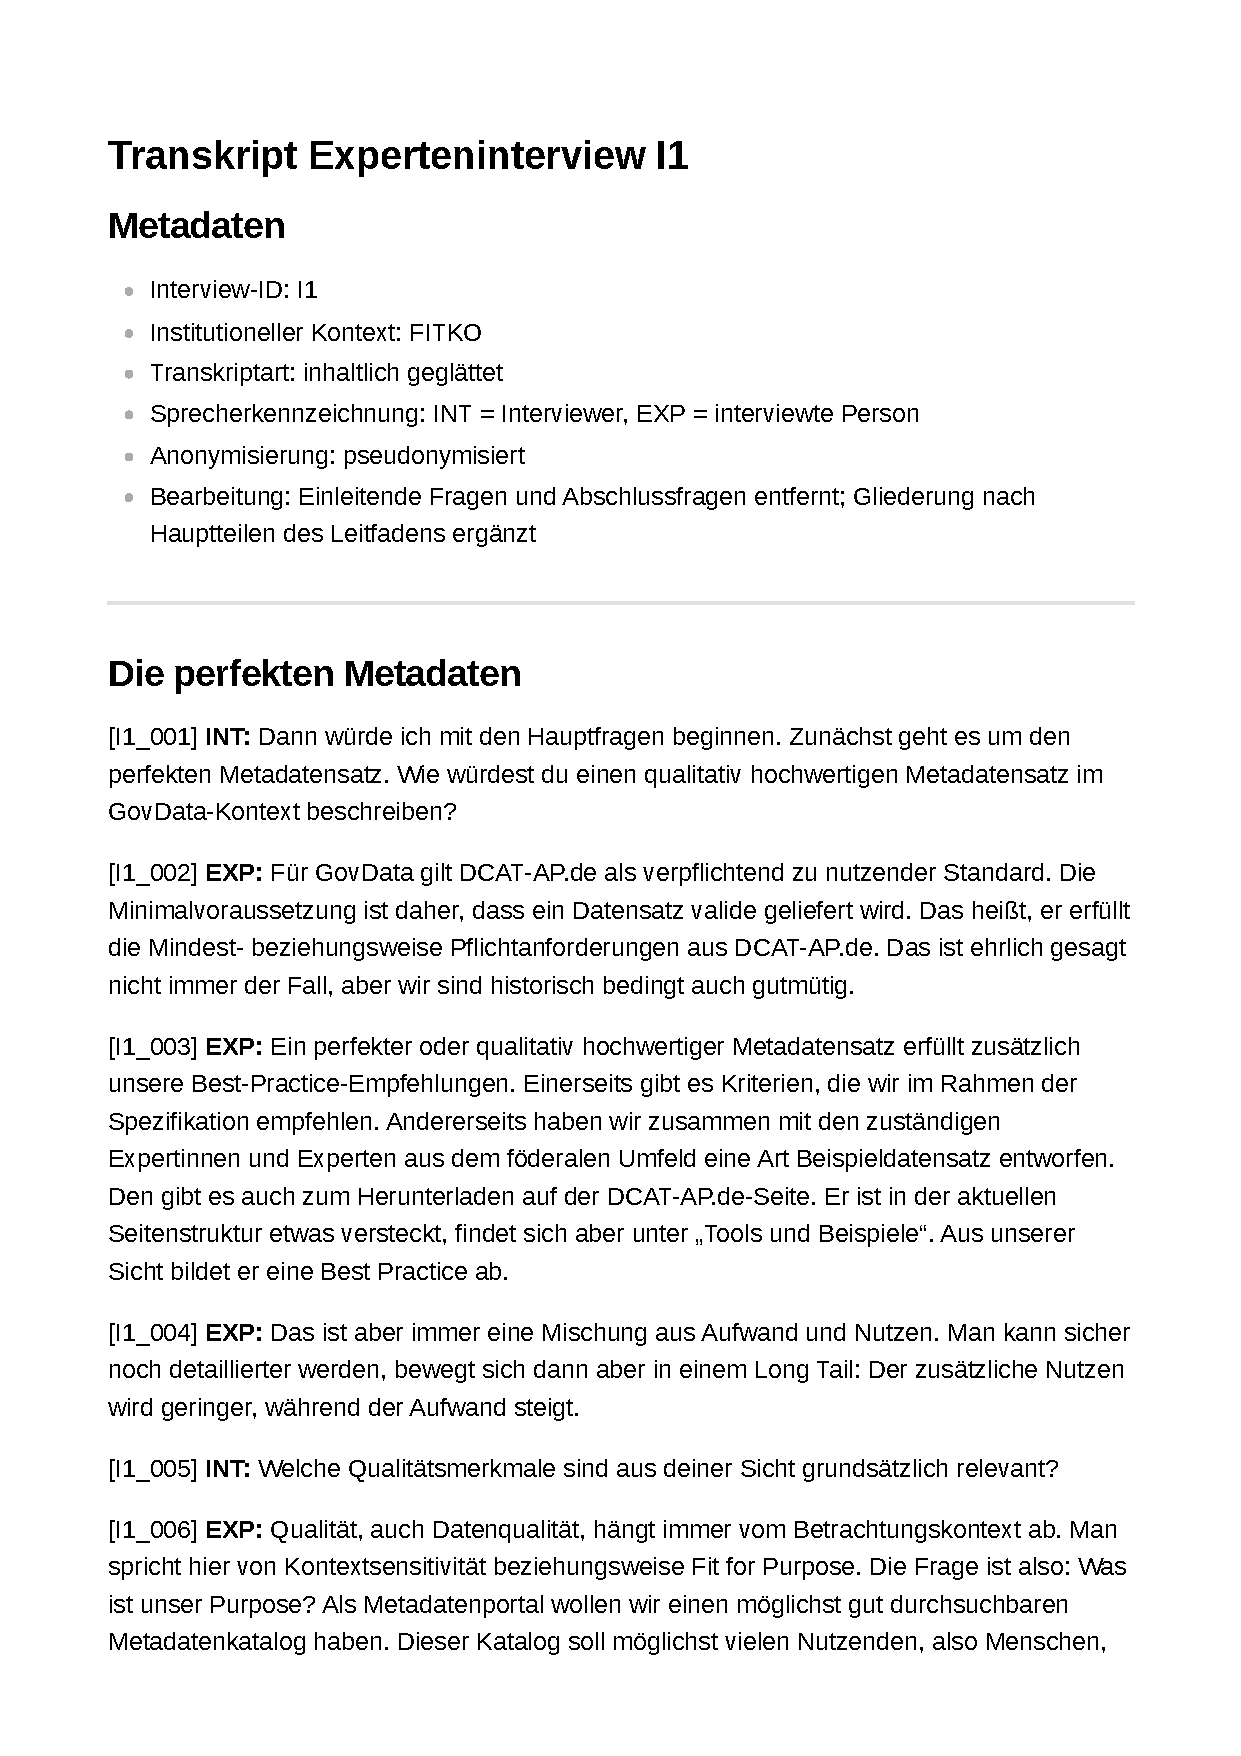
\includepdf[pages=-]{appendix/I1_transkript_bereinigt.pdf}

\chapter{Transkript Interview 2}
\label{app:transkript_i2}
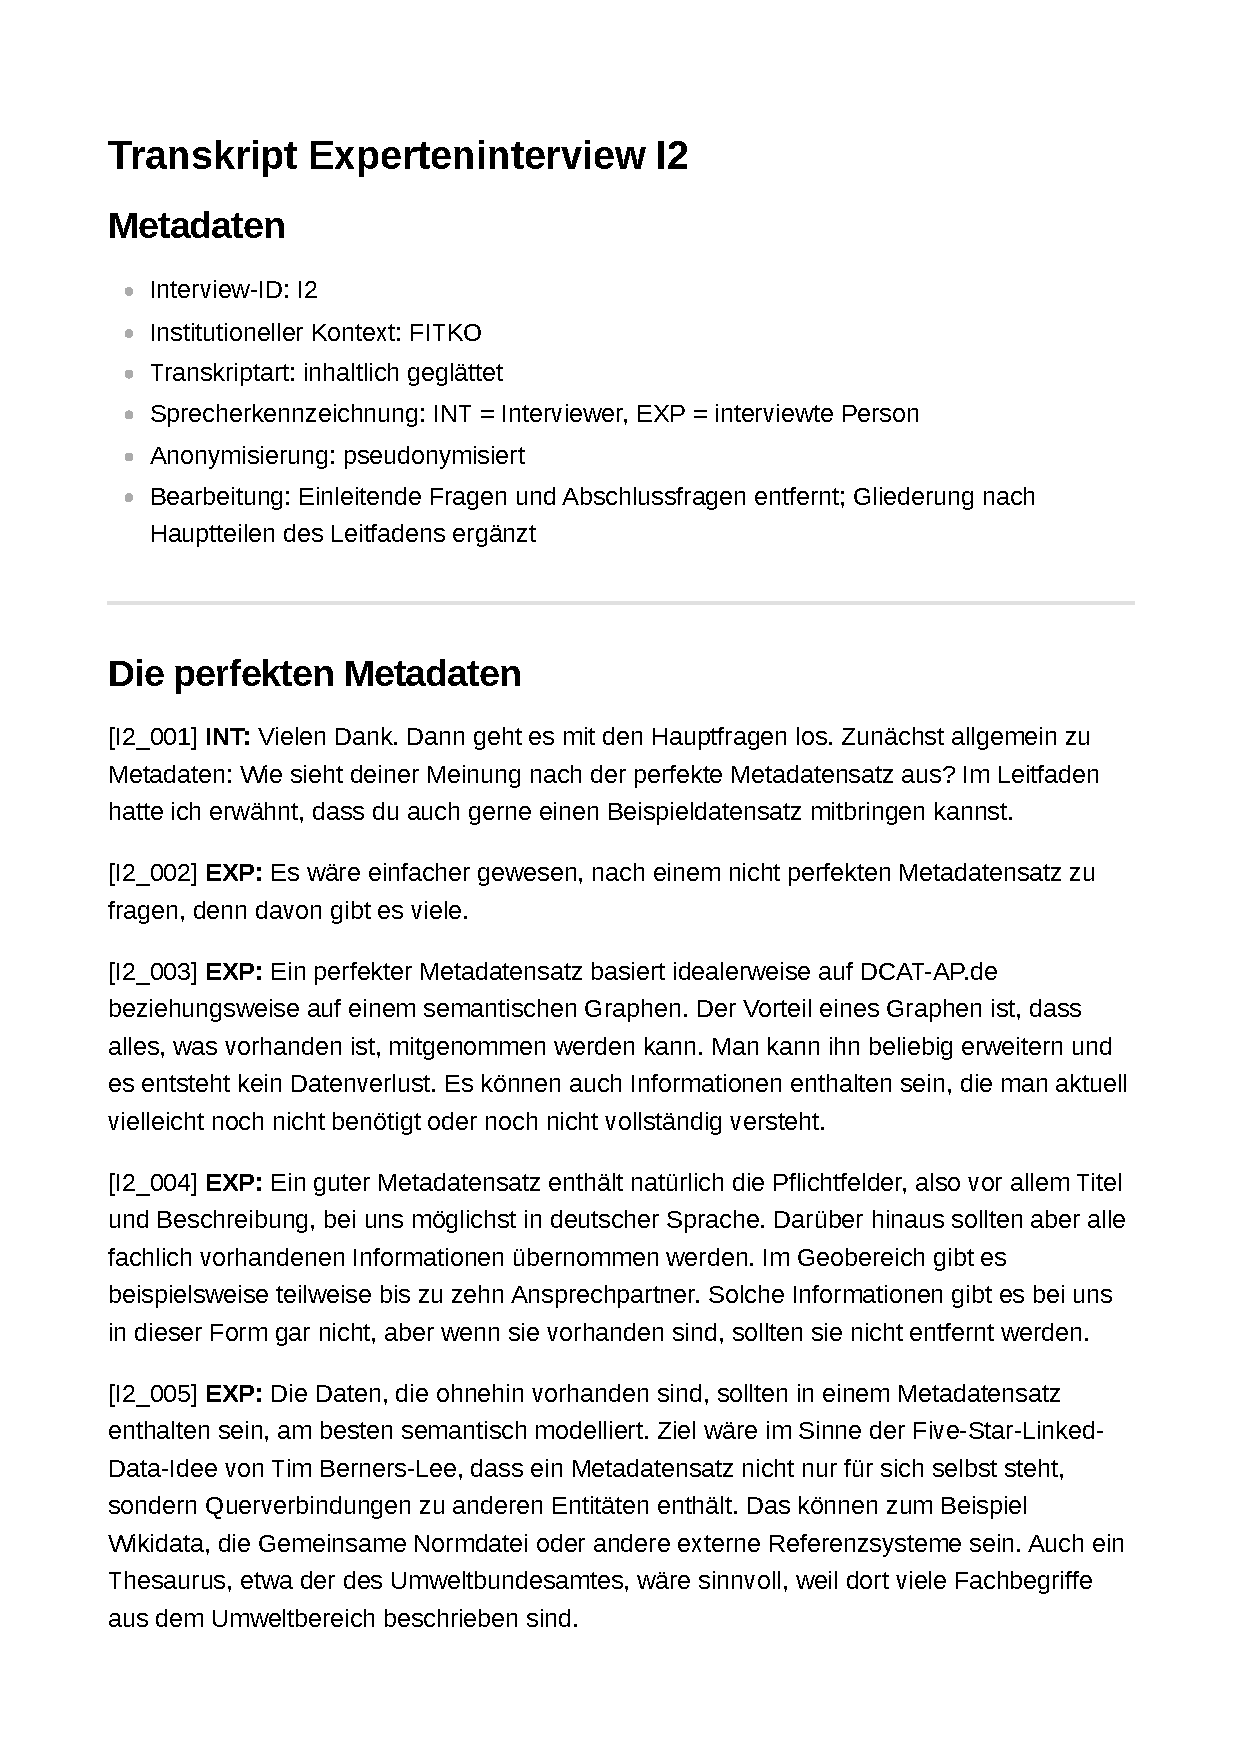
\includepdf[pages=-]{appendix/I2_transkript_bereinigt.pdf}

\chapter{Transkript Interview 3}
\label{app:transkript_i3}
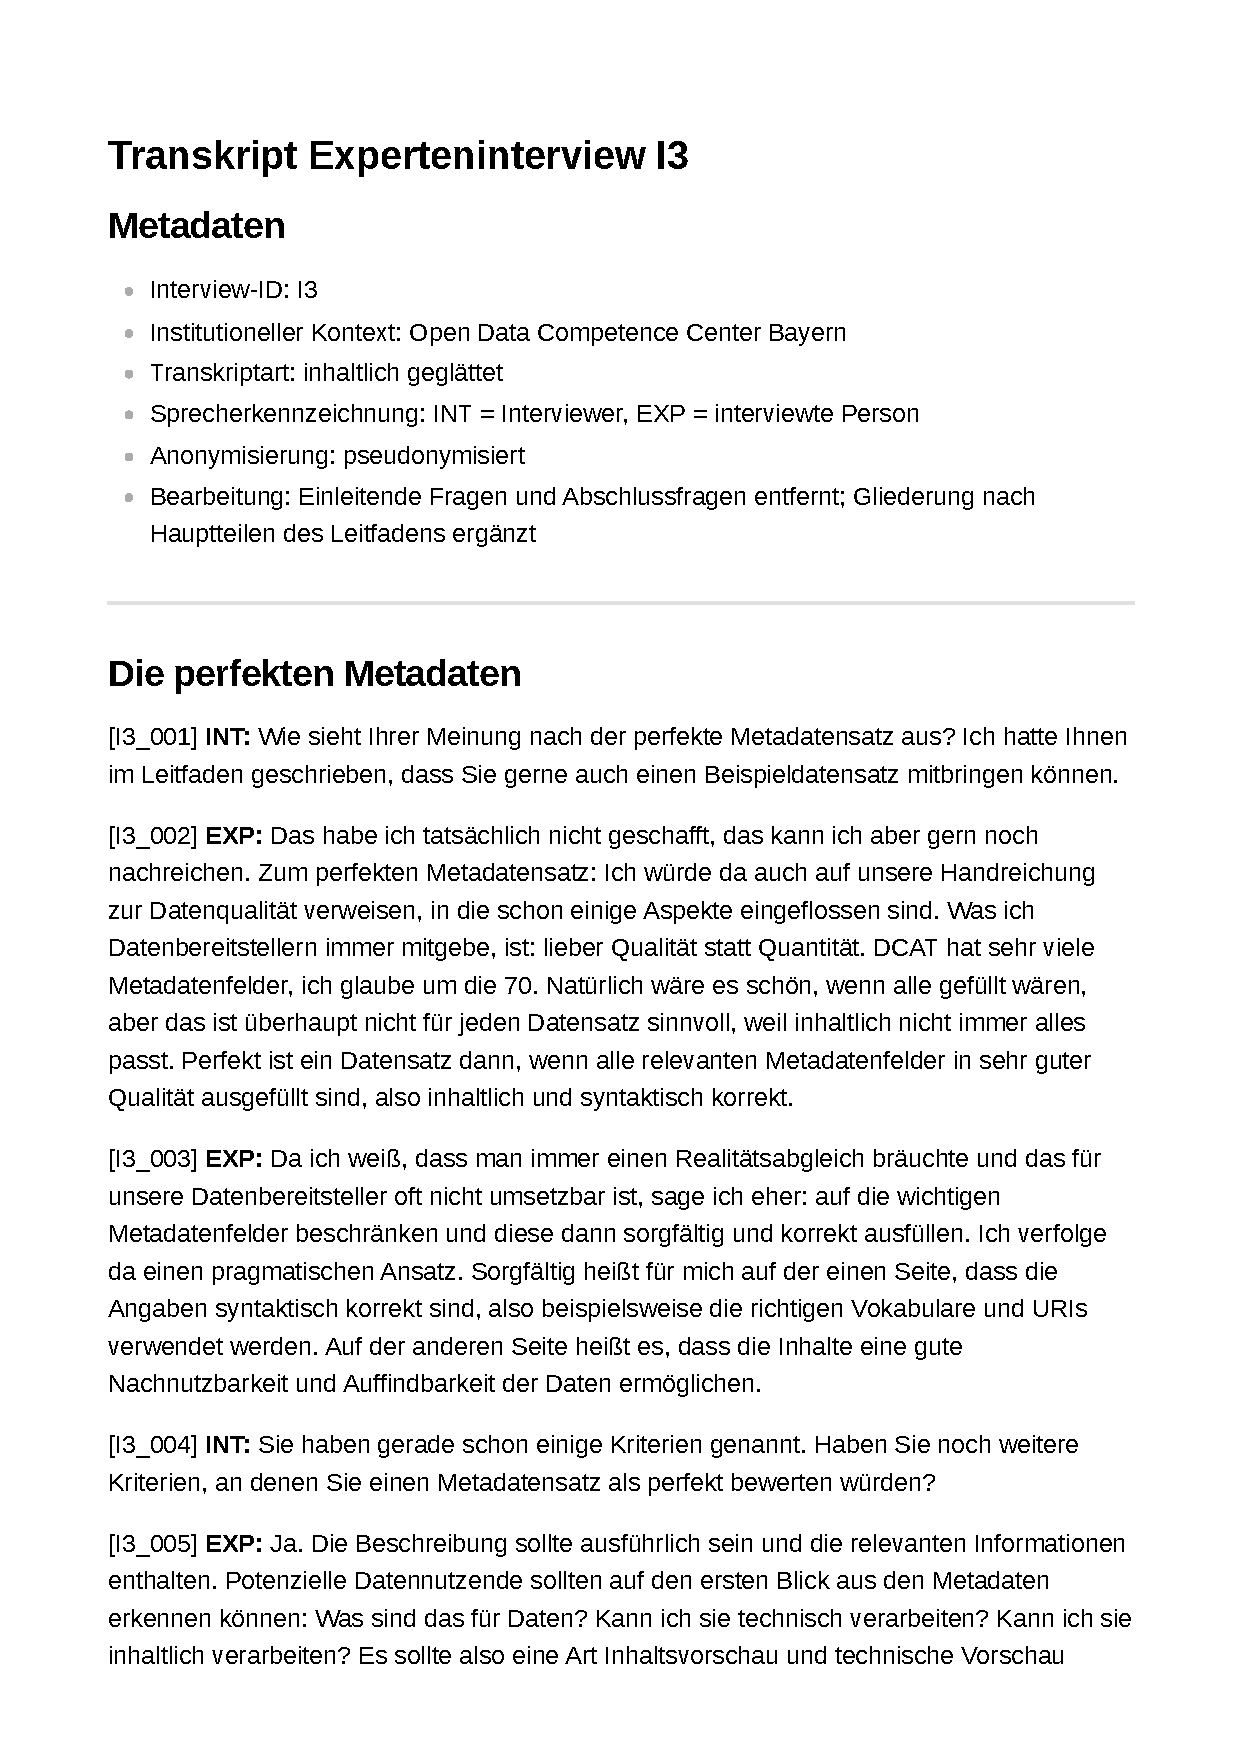
\includepdf[pages=-]{appendix/I3_transkript_bereinigt.pdf}

\chapter{Kodierte Auswertungsmatrix der Interviews}
\label{app:kodierte_auswertungsmatrix}
\begingroup
\tiny
\renewcommand{\arraystretch}{1.05}
\setlength{\LTleft}{-1.0cm}
\setlength{\LTright}{0pt}

\begin{longtable}{p{0.9cm} p{6cm} p{0.9cm} p{0.9cm} p{6cm}}
\caption{Codierte Auswertungsmatrix der Experteninterviews}
\label{tab:codierte-auswertungsmatrix}\\

\toprule
\textbf{Fundstelle} & \textbf{Paraphrase der Aussage} & \textbf{Primär\-code} & \textbf{Sekun\-där\-code} & \textbf{Analytische Notiz / Modellfolge} \\
\midrule
\endfirsthead

\toprule
\textbf{Fundstelle} & \textbf{Paraphrase der Aussage} & \textbf{Primär\-code} & \textbf{Sekun\-där\-code} & \textbf{Analytische Notiz / Modellfolge} \\
\midrule
\endhead

\midrule
\multicolumn{5}{r}{\textit{Fortsetzung auf der nächsten Seite}} \\
\midrule
\endfoot

\bottomrule
\endlastfoot

\multicolumn{5}{l}{\textbf{Interview I1}} \\
\midrule
I1\_002 & DCAT-AP.de-Validität wird als Mindestvoraussetzung hochwertiger GovData-Metadaten beschrieben. & K3.1 & K1.1 & Basiskonformität als Mindestanforderung im Modell ausweisen. \\
I1\_003 & Best-Practice-Empfehlungen und Beispieldatensätze markieren eine höhere Qualitätsstufe jenseits der Mindestvalidität. & K1.1 & K2.2 & Pflicht- und Best-Practice-Erfüllung getrennt bewerten. \\
I1\_004 & Zusätzliche Detailtiefe steht in einem Aufwand-Nutzen-Verhältnis mit abnehmendem Grenznutzen. & K1.2 & K7.5 & Score nicht durch maximale Feldanzahl überladen. \\
I1\_006 & Datenqualität wird als kontextsensitiv und zweckabhängig beschrieben; GovData soll Auffindbarkeit und Zugang erleichtern. & K7.1 & K1.3 & Bewertung an Nutzungskontext und Such-/Zugriffsfunktion ausrichten. \\
I1\_007 & Reichhaltigkeit und Vollständigkeit der Metadaten gelten als zentrale Qualitätskriterien. & K2.2 & K2.1 & Empfohlene Felder und Reichhaltigkeit im Score berücksichtigen. \\
I1\_009 & Optionale Rollen wie Creator oder Maintainer sind je nach Domäne unterschiedlich relevant. & K7.1 & K2.3 & Domänenspezifische Feldgewichtung ermöglichen. \\
I1\_010 & Allgemeine DCAT-AP.de-Eigenschaften sind breit relevant, spezifische Relationen stärker kontextabhängig. & K7.1 & K2.4 & Unterscheidung zwischen allgemeinen und kontextspezifischen Indikatoren. \\
I1\_012 & Föderale Portale unterscheiden sich in Leistungsfähigkeit und Veröffentlichungsprozessen. & K7.3 & K9.4 & Vergleichbarkeit zwischen Portalen vorsichtig kontextualisieren. \\
I1\_013 & Kontextsensitive Beispieldatensätze werden genutzt, um thematische Vielfalt sichtbar zu machen. & K7.1 & K4.3 & Evaluation mit thematisch unterschiedlichen Datensätzen planen. \\
I1\_014 & Schleswig-Holstein wird wegen vorgeschalteter Qualitätssicherung und Best-Practice-Umsetzung als positiver Referenzpunkt genannt. & K1.1 & K9.4 & Gute Beispiele als Benchmark für Modelltests nutzen. \\
I1\_015 & Schlecht gepflegte, veraltete, unklare oder nicht erreichbare Datensätze werden als typische Qualitätsprobleme beschrieben. & K5.1 & K4.4 & Verfügbarkeit und Beschreibungsklarheit als zentrale Prüffelder einbauen. \\
I1\_017 & Bestehende Scores sollten stärker an etablierten Datenqualitätskriterien und Fit-for-Purpose-Konzepten anknüpfen. & K9.1 & K7.1 & Indikatorenauswahl theoretisch begründen. \\
I1\_018 & Klassische Datenqualitätskriterien werden als leicht nutzbare Grundlage für Analysewerkzeuge beschrieben. & K9.1 & K3.5 & Literaturbasierte Basisdimensionen in das Modell integrieren. \\
I1\_019 & Funktionierende Links, Fehlerfreiheit, Alter, Aktualisierung und Harvesting-Zeitpunkt sind relevante Basiskriterien. & K5.3 & K7.5 & Aktualität und Harvesting als eigene Kontextindikatoren prüfen. \\
I1\_020 & Linked-Data-Qualität wird über intensive RDF-Nutzung, Vokabularverweise und IDs statt Literale beschrieben. & K6.1 & K6.3 & Linked-Data-Reife als Qualitätsdimension aufnehmen. \\
I1\_022 & Eine GND-ID wird als verlässlicher bewertet als derselbe Name als Freitextliteral. & K6.1 & K6.2 & Normdatenbezug als Verlässlichkeitsindikator operationalisieren. \\
I1\_024 & Harvesting- und Katalog-Metadaten werden als interne Qualitätskriterien für GovData beschrieben. & K5.3 & K9.1 & Catalog-Record-Informationen als mögliche Zusatzdimension prüfen. \\
I1\_025 & Catalog Records könnten Validierungen, Harvesting-Herkunft und Aktualisierungsinformationen dokumentieren. & K5.3 & K6.3 & Katalog-Metadaten für Qualitätsnachweise nutzen. \\
I1\_027 & DCAT-AP.de-Validierung wird als wichtige Basis unter Fehlerfreiheit eingeordnet. & K3.2 & K9.2 & SHACL/Validierung als formale Basiskomponente verwenden. \\
I1\_028 & Validierung ist wichtig, aber nicht ausreichend; Syntax, formale und inhaltliche Qualität benötigen unterschiedliche Methoden. & K9.2 & K4.4 & Formale und semantische Teildimensionen getrennt ausweisen. \\
I1\_029 & DCAT-AP.de-Qualität soll als Dimension im Gesamtscoring angezeigt werden, Gewichtung bleibt schwierig. & K9.2 & K3.2 & SHACL nicht als Gesamtscore interpretieren. \\
I1\_031 & Stark normierte Ausgangsdaten, insbesondere Geodaten, erleichtern hochwertige Metadaten. & K7.2 & K8.5 & Domänenspezifische Ausgangslage bei Bewertung berücksichtigen. \\
I1\_032 & Die Grenze zwischen Daten und Metadaten ist fließend; normierte Bereiche bieten reichhaltige Informationen. & K8.5 & K7.2 & Rohdatenbezug domänenspezifisch begrenzen. \\
I1\_033 & Freie, einzigartige oder manuell erhobene Daten sind schwieriger gut zu beschreiben. & K7.1 & K4.4 & Beschreibungsgüte abhängig vom Datentyp interpretieren. \\
I1\_035 & Freitext und natürliche Sprache bieten Potenzial für LLM-/KI-gestützte Fehler- und Schwächenanalyse. & K10.2 & K3.5 & KI für Freitext- und einfache Plausibilitätsprüfungen prüfen. \\
I1\_036 & KI kann fehlertolerant unterstützen, ersetzt aber teilweise nur klassisch mögliche Verfahren. & K10.1 & K10.9 & KI-Einsatz nur bei zusätzlichem Nutzen rechtfertigen. \\
I1\_037 & Kontextsensitive semantische KI-Analyse kann fachliche Begriffe fehlinterpretieren und Schaden erzeugen. & K10.8 & K4.3 & Keine autonome Korrektur fachsprachlicher Metadaten. \\
I1\_039 & Eine agentische KI könnte als Metadaten-Linter auf Basis von DCAT-AP.de, SHACL und Soll-/Kann-Kriterien dienen. & K10.1 & K3.2 & Linter-Funktion als unterstützendes Analysemodul konzipieren. \\
I1\_040 & KI kann Lücken identifizieren und föderale Vergleichbarkeit zwischen ähnlichen Datensätzen unterstützen. & K7.3 & K10.6 & Vergleichsanalyse als KI-unterstützte Kontextfunktion. \\
I1\_041 & Assisted Learning kann Freitext-Stichworte auf Kategorien, Schlagworte oder EU-Vokabulare mappen. & K10.3 & K6.3 & Keyword-Harmonisierung als potenzieller KI-Indikator. \\
I1\_043 & KI ist bei natürlicher Sprache, einfacher Sprache, Barrierearmut, Fachtermini und Synonymen sinnvoll. & K10.2 & K4.3 & Verständlichkeits- und Synonymprüfung als KI-gestützte Ergänzung. \\
I1\_044 & KI kann Beschreibungstexte anhand von Style Guides prüfen und Verbesserungsvorschläge machen. & K10.2 & K9.5 & KI nur als Vorschlags- und Verbesserungsebene nutzen. \\
I1\_046 & Generative KI ist für Scoring problematisch, da stochastische Ausreißer und hoher Wiederholungsaufwand entstehen. & K10.8 & K10.9 & KI nicht als autonome Bewertungsinstanz einsetzen. \\
I1\_047 & Qualitätsfragen erfordern häufig spezifische SPARQL-Abfragen; Stakeholder haben unterschiedliche Bedarfe. & K10.4 & K7.4 & SPARQL-Assistenz für domänenspezifische Qualitätsfragen prüfen. \\
I1\_048 & Regionale Datentypen benötigen angepasste Queries und spezifische Analysebausteine. & K10.4 & K7.1 & Templates oder KI-Assistenz für kontextspezifische Abfragen nutzen. \\
I1\_049 & KI kann Fachpersonen ohne tiefe technische Expertise Zugang zu Auswertungen geben. & K10.4 & K7.4 & Assistenzsystem statt autonomem Score-Generator vorsehen. \\
\multicolumn{5}{l}{\textbf{Interview I2}} \\
\midrule
I2\_002 & Nicht perfekte Metadaten werden als häufiges Praxisphänomen beschrieben. & K1.1 & K9.5 & Modell muss typische Fehler verständlich erfassen. \\
I2\_003 & Perfekte Metadaten basieren idealerweise auf DCAT-AP.de beziehungsweise einem semantischen Graphen. & K1.4 & K6.4 & Graphfähigkeit als Idealstruktur berücksichtigen. \\
I2\_004 & Pflichtfelder sind notwendig; fachlich vorhandene Informationen sollten zusätzlich übernommen werden. & K2.3 & K2.2 & Feldreichhaltigkeit über Pflichtfelder hinaus bewerten. \\
I2\_005 & Semantische Modellierung, externe Referenzen, Wikidata, GND und Thesauri werden als Ideal genannt. & K6.2 & K6.3 & Externe Referenzierung und Thesaurusnutzung prüfen. \\
I2\_006 & Querverbindungen zwischen vergleichbaren kommunalen Datensätzen werden als Idealfall beschrieben. & K6.4 & K7.3 & Interlinking zwischen vergleichbaren Datensätzen als Qualitätsaspekt. \\
I2\_008 & Zu kurze Titel und identische Titel/Beschreibungen machen Metadaten unverständlich. & K4.1 & K4.2 & Titelqualität und Redundanzprüfung aufnehmen. \\
I2\_009 & Regionale Begriffe wie „I-Dötzchen“ erschweren die Verständlichkeit. & K4.3 & K10.2 & Regionale Begriffe und Synonyme als Freitextproblem berücksichtigen. \\
I2\_010 & Fachsprache kann detailliert und korrekt, aber für Außenstehende unverständlich sein. & K4.3 & K4.4 & Verständlichkeitsprüfung nicht mit fachlicher Korrektheit verwechseln. \\
I2\_011 & Dead Links, zu wenige Metadaten und widersprüchliche Angaben werden als schlechte Metadaten beschrieben. & K5.1 & K4.5 & Verfügbarkeit und Plausibilität getrennt prüfen. \\
I2\_012 & Eigentliche Daten sind oft aussagekräftiger als menschlich eingetragene Metadaten. & K8.3 & K8.5 & Rohdaten als ergänzende Prüfbasis berücksichtigen. \\
I2\_013 & Bounding Boxes sind manuell eingetragen und fehleranfällig; Berechnung aus Daten wäre sinnvoller. & K8.4 & K7.2 & Geobezogene Angaben aus Daten ableiten oder validieren. \\
I2\_014 & Metadatenfehler entstehen häufig, weil Bereitstellende Zweck und Nachnutzung nicht verstehen. & K1.3 & K9.5 & Reporting muss Zweck und Nutzen von Feldern erklären. \\
I2\_016 & Praxiskenntnis vieler guter und schlechter Datensätze wird bestätigt. & K9.4 & K1.1 & Evaluation mit Beispieldatensätzen stützen. \\
I2\_017 & Portalübergreifende Verarbeitung kann Dubletten und technische Verschlechterungen erzeugen. & K6.4 & K5.2 & Provenienz und Datensatzidentität stärker berücksichtigen. \\
I2\_020 & Diskussionen zu Scores betreffen besonders wissenschaftliche und semantische Grundlagen. & K9.1 & K4.6 & Kriterien theoretisch und semantisch begründen. \\
I2\_021 & Aktuelle Scores prüfen oft ohne ausreichend begründete wissenschaftliche Grundlage. & K9.1 & K1.1 & Kriterienauswahl im Modell transparent begründen. \\
I2\_022 & EU- und Schweizer Scores werden wegen fehlender Begründung trotz FAIR-Bezug kritisiert. & K9.1 & K2.2 & Übernommene Metriken nicht unreflektiert verwenden. \\
I2\_023 & GovData will Qualität sinnvoll messen; was gemessen wird, muss geklärt sein. & K9.1 & K9.3 & Indikatoren vor Scoringlogik konzeptionell begründen. \\
I2\_024 & Reine Anzahl von Datensätzen ist als Erfolgs- oder Qualitätsmetrik ungeeignet. & K9.1 & K1.2 & Keine quantitätsgetriebene Portallogik als Qualitätsersatz. \\
I2\_026 & Absolute Vollständigkeit ist im Graphen unmöglich; relevant ist relative Vollständigkeit je Fachthema. & K2.1 & K7.1 & Vollständigkeit relational und domänenspezifisch interpretieren. \\
I2\_027 & Sprachliche Verständlichkeit ist zentral; Länge allein reicht nicht. & K4.4 & K10.2 & Beschreibungsgüte semantisch statt nur formal prüfen. \\
I2\_028 & Distributionen sollten verschiedene Formate derselben Daten korrekt beschreiben. & K5.2 & K8.1 & Distributionen und Formatbeschreibung prüfen. \\
I2\_029 & Blank Nodes vermeiden, Querverweise nutzen und Organisationen strukturiert abbilden. & K6.5 & K6.4 & Strukturelle Linked-Data-Qualität einbeziehen. \\
I2\_030 & Attribution und korrekte Quellenangabe bei Lizenzen gehören zur Metadatenqualität. & K4.6 & K7.4 & Lizenz- und Attributionsangaben als Reuse-Kontext prüfen. \\
I2\_031 & Der Weg eines Datensatzes durch verschiedene Portale ist derzeit nicht sauber abbildbar. & K5.3 & K6.4 & Provenienz/Harvesting-Pfad als Zusatzinformation erwägen. \\
I2\_032 & Verbesserung von Metadaten durch Portale wirft Fragen der Datenhoheit auf. & K10.7 & K9.5 & Automatische Korrektur von Analyse und Empfehlung trennen. \\
I2\_034 & SHACL-/Qualitätsrankings können für Ländervertretungen und Bund nützlich sein. & K9.4 & K9.2 & Benchmarking als Verbesserungsinstrument möglich. \\
I2\_035 & Länder und Kommunen möchten sich vergleichen und Ressourcenbedarf sichtbar machen. & K9.4 & K7.3 & Vergleiche kontextualisiert bereitstellen. \\
I2\_036 & Rankings sollen nicht bloßstellen, sondern Hinweise auf Verbesserungsmöglichkeiten geben. & K9.5 & K9.4 & Reporting handlungsorientiert formulieren. \\
I2\_037 & Regelmäßige Prüfungen können dazu führen, dass Fehler behoben werden. & K9.4 & K5.3 & Wiederholte Prüfung als Monitoringfunktion einplanen. \\
I2\_039 & Teil-Scores helfen, Problembereiche zu lokalisieren. & K9.3 & K9.5 & Mehrdimensionale Teilscores statt nur Gesamtscore. \\
I2\_040 & SHACL-Ergebnisse sind häufig technisch und müssen interpretiert werden. & K9.5 & K3.2 & Validatorausgaben in verständliches Reporting übersetzen. \\
I2\_041 & Fehlermeldungen müssen erklären, was konkret zu tun ist. & K9.5 & K3.4 & Handlungshinweise pro Fehlerklasse entwickeln. \\
I2\_043 & Grenze zwischen Metadaten und Daten verschwimmt im GovData-Kontext. & K8.5 & K1.4 & Rohdatenbezug methodisch abgrenzen. \\
I2\_044 & Geodatenservices sind APIs, die sich selbst beschreiben und Daten unter der Metadatenebene enthalten. & K8.2 & K7.2 & Services anders bewerten als statische Dateien. \\
I2\_045 & Metadaten und Daten korrelieren; falsche Formatangaben verletzen Metadatenqualität. & K8.1 & K5.4 & Formatabgleich als automatisierbarer Indikator. \\
I2\_046 & Erwartetes und tatsächliches Serviceverhalten kann auseinanderfallen, etwa Karte versus XML-Fehlermeldung. & K8.2 & K5.2 & Service-Output gegen Nutzungserwartung prüfen. \\
I2\_047 & Titel und tatsächlicher Dateninhalt können nicht zusammenpassen. & K8.3 & K4.5 & Inhaltliche Metadaten-Daten-Kongruenz prüfen. \\
I2\_049 & AI Agents sollten nicht von vornherein in den Vordergrund gestellt werden. & K10.8 & K10.1 & KI-Einsatz fachlich begründen. \\
I2\_050 & Vor KI-Einsatz ist zu prüfen, ob andere Mittel dasselbe Problem lösen können. & K10.9 & K9.1 & KI nur bei methodischem Mehrwert einsetzen. \\
I2\_051 & AI Agents sind nicht automatisch intelligent; entscheidend ist die Art der Ansteuerung. & K10.8 & K10.1 & Automatisierungsgrad begrenzen. \\
I2\_052 & Textanalyse ist schwach; KI auf semantischem Graphen ist verlässlicher und halluziniert weniger. & K10.5 & K10.8 & Graphbasierte KI statt rein textbasierter KI bevorzugen. \\
I2\_054 & Agenten könnten Graphen, europäische Portale und wissenschaftliche Portale als Kontext heranziehen. & K10.5 & K6.2 & Externe Kontexte kontrolliert einbeziehen. \\
I2\_055 & Schlagwörter sind oft Zeichenketten; Thesauri können zusätzlichen Kontext liefern. & K6.3 & K10.3 & Keyword-Kontextualisierung über Vokabulare unterstützen. \\
I2\_056 & Verwandte Konzepte im Graphen verbessern Suche und Bewertung. & K6.4 & K10.5 & Graphbasierte semantische Kontextanalyse ermöglichen. \\
I2\_058 & Portale sollten stärker in die Daten selbst hineinschauen, um Passung zu prüfen. & K8.3 & K10.6 & Rohdatenprüfung als Erweiterung des Scorings. \\
I2\_059 & Agenten könnten Strukturen, Vergleichbarkeit und Flächendeckung prüfen. & K10.6 & K8.4 & KI für komplexe Rohdatenmuster prüfen. \\
I2\_060 & KI kann große Datenmengen, ältere Sprachmuster und historische Kontexte analysieren. & K10.6 & K4.3 & KI für Massenauswertung und Sprachkontext nutzbar. \\
I2\_061 & Häufigkeiten in großen Datensatzmengen sind manuell kaum analysierbar. & K10.6 & K9.3 & Skalierende Analysebausteine vorsehen. \\
I2\_062 & KI erzeugt Serverlast und benötigt Training sowie Betrieb. & K10.9 & K10.8 & Betriebskosten und Infrastruktur als Grenze einplanen. \\
I2\_063 & KI ist sinnvoll, aber nicht alles muss mit KI gelöst werden. & K10.9 & K9.1 & Aufwand-Nutzen-Prüfung in KI-Konzept aufnehmen. \\
\multicolumn{5}{l}{\textbf{Interview I3}} \\
\midrule
I3\_002 & Perfekte Metadaten enthalten relevante Felder in hoher inhaltlicher und syntaktischer Qualität; nicht alle Felder sind immer sinnvoll. & K1.2 & K2.4 & Relevanzbasierte statt maximale Feldbefüllung. \\
I3\_003 & Wichtige Felder sollen sorgfältig, syntaktisch korrekt und nachnutzbar ausgefüllt sein. & K2.4 & K3.3 & Syntaktische Korrektheit und Nachnutzbarkeit verbinden. \\
I3\_005 & Metadaten sollen Inhalts- und technische Vorschau bieten, bevor der Datensatz geöffnet wird. & K1.3 & K4.4 & Nutzungsentscheidung durch Metadaten ermöglichen. \\
I3\_006 & Konsistenz und Standardisierung sind bei ähnlichen Daten wichtig, etwa Einwohnerstatistiken. & K4.6 & K6.3 & Synonym- und Standardisierungsprobleme berücksichtigen. \\
I3\_008 & Schlechte Metadaten finden sich sowohl auf GovData als auch im eigenen Portal. & K1.1 & K9.4 & Breite Testbasis für Prototyp möglich. \\
I3\_010 & piveau prüft Feldexistenz, Validator Syntax; inhaltliche Sinnhaftigkeit bleibt unberücksichtigt. & K4.4 & K9.1 & Semantische Qualität als Ergänzung bestehender Ansätze. \\
I3\_012 & Scoring sollte mehrstufig prüfen: Existenz, syntaktische Korrektheit, semantische und inhaltliche Passung. & K9.3 & K3.4 & Mehrstufige Bewertungsarchitektur ableiten. \\
I3\_013 & Pflichtfelder allein reichen nicht; auch über DCAT-Pflichtfelder hinausgehende Felder sind relevant. & K2.2 & K2.4 & Empfohlene und weitere relevante Felder berücksichtigen. \\
I3\_015 & Validierung verbindet Feldexistenz mit syntaktisch korrekter Ausfüllung. & K3.2 & K3.4 & SHACL als Verbindung von Vollständigkeit und Syntax nutzen. \\
I3\_017 & Validierungsergebnisse sollen klar trennen, ob ein Feld fehlt oder syntaktisch fehlerhaft ist. & K3.4 & K9.5 & Fehlerarten explizit im Report ausweisen. \\
I3\_018 & Valides XML, korrekte URIs und Vokabulare sind grundlegende Prüfungen. & K3.5 & K3.3 & Basale technische Prüfungen als harte Kriterien. \\
I3\_020 & Rohdaten sind für Gegenprüfung relevant; falsche Formatangaben zeigen Metadatenfehler. & K8.1 & K5.4 & Formatkongruenz als automatisierbarer Indikator. \\
I3\_021 & Rohdatenqualität betrifft nicht-proprietäre und gut lesbare Formate, wird aber auch an Bereitstellende herangetragen. & K5.4 & K8.5 & Rohdatenqualität nur angrenzend berücksichtigen. \\
I3\_022 & Metadatenportale können Rohdaten fachlich nur begrenzt bewerten; Fachstandards unterscheiden sich. & K8.5 & K7.2 & Fachliche Grenzen des Modells transparent machen. \\
I3\_024 & Kontextsensitive KI kann Rohdaten und Umfeld nutzen, um Metadaten über Syntax hinaus zu prüfen. & K10.6 & K8.3 & KI-gestützte Kontextprüfung als Erweiterung prüfen. \\
I3\_026 & Große Mengen könnten schneller bewertet werden; Datenhoheit bei Veränderung bleibt kritisch. & K10.7 & K10.9 & Messung von automatischer Veränderung trennen. \\
I3\_028 & Format, Dateigröße, zeitliche Bezüge, Titel, Beschreibung, Keywords, Themenfeld und Kategorie sind relevante Prüfinformationen. & K8.1 & K4.6 & Technische und semantische Kontextfelder operationalisieren. \\
I3\_029 & Lizenz, Publisher und Contact Point sind wichtig, aber schwer kontextsensitiv automatisiert zu prüfen. & K8.5 & K7.4 & Rechtliche und Herkunftsfelder vorsichtig bewerten. \\
I3\_031 & Weitere KI-Anwendungsfälle werden nicht konkret benannt. & K10.9 &  & Kein zusätzlicher Indikator; als negative Evidenz dokumentieren. \\

\end{longtable}

\end{document}